% 高一43_交附闵行_周练3.tex
%   —— 高一上数学“2026-2027 年交附闵行高一上周练3”（试卷版/答案版）
% 试卷版：xelatex 高一43_交附闵行_周练3.tex
% 答案版：xelatex "\def\isanswer{1}% 高一43_交附闵行_周练3.tex
%   —— 高一上数学“2026-2027 年交附闵行高一上周练3”（试卷版/答案版）
% 试卷版：xelatex 高一43_交附闵行_周练3.tex
% 答案版：xelatex "\def\isanswer{1}% 高一43_交附闵行_周练3.tex
%   —— 高一上数学“2026-2027 年交附闵行高一上周练3”（试卷版/答案版）
% 试卷版：xelatex 高一43_交附闵行_周练3.tex
% 答案版：xelatex "\def\isanswer{1}% 高一43_交附闵行_周练3.tex
%   —— 高一上数学“2026-2027 年交附闵行高一上周练3”（试卷版/答案版）
% 试卷版：xelatex 高一43_交附闵行_周练3.tex
% 答案版：xelatex "\def\isanswer{1}\input{高一43_交附闵行_周练3.tex}"
% 紧凑版：xelatex "\def\iscompact{1}\input{高一43_交附闵行_周练3.tex}"
%
% 原始材料是微信公众号图文（公众号“魔都数学加油站”，作者破晓，2026-10-01 21:37，
% 原文标题“27学年高一43——2026-2027年上海市交附闵行高一上周练3”，
% https://mp.weixin.qq.com/s/-rgkOD9jJVpug6s0uSbwmQ）。正文为 12 张 PNG 页；
% 第 01、05、09、12 页 2560×3620，其余第 02—04、06—08、10—11 页 4762×6735。
% 原文本身是讲评版，题目下方印有解析/答案；题目与讲解照原卷转录，保留原卷错误。
%
% 卷首标题：原卷印作“2026-2027 年交附闵行高一上周练3”，公众号标题中的“上海市”
% 三字不在卷面标题中，本稿依卷面录入；年份区间按全稿惯例排 en dash。
%
% 与原卷的排版差异：
%   ① 原文从第 3 题开始（第 1、2 题未在这篇推文中发布），本稿保留原题号 3—21；
%   ② 原卷本就印有“一、填空题”“二、选择题”“三、解答题”，本稿照原卷分节，
%      改排为全稿统一的大节标题；
%   ③ 原卷未印副标题，本稿按“知识模块”口径补出“集合与常用逻辑用语、不等式”；
%   ④ 原卷填空横线依全稿惯例排为 \blankline[4.4em]；选择题答案只在答案版以 \ans{} 显示，
%      解答区以 \ifanswer 分离；解答题按原卷留出标准作答空间；
%   ⑤ 第 5 题图取自原卷第 1 页截图并裁入本稿，不另建图档；公众号水印不录入。
%      原卷图页分页不保留，正文依本稿版心重新分页。
%
% 原卷存疑/错误（均照录，未改）：
%   ① 第 9 题原卷题干即作"正实数 x、y"，与解析 x>0、y>0 相容，并无矛盾（初稿曾误记
%      题干只称"实数"并据此指原卷不自洽，2026-10-05 回原图核对订正）。
%   ② 第 11 题解析"相加得"一行原卷印作 -2<3/5(a+2b)+1/5(2a-b)<2，第一项系数 3/5
%      原卷不缺（初稿漏抄致该行按字面不成立，2026-10-05 已按原卷补回）。
%   ③ 第 13 题答案印 A，解析以“1-k≠0”排除 k=1；但 k=1 时原方程为 -2x-1=0，
%      仍有实数根，按题意应选 B。本稿保留原卷答案 A 及其解析，不代为订正。
%
\documentclass[a4paper,11pt]{article}
\usepackage{common}
\usepackage{graphicx}

\begin{document}

\examtitlest[3]{2026--2027 年交附闵行高一上周练 3}{集合与常用逻辑用语、不等式}

\bigsec{一、填空题}

\begin{enumerate}
\setcounter{enumi}{2}

\item 已知 $p\colon -2\leqslant x\leqslant10$，$q\colon 1-m\leqslant x\leqslant1+m$（$m>0$）. 若 $p$ 是 $q$ 的充分不必要条件，则实数 $m$ 的取值范围是 \blankline[4.4em].

\ifanswer
\solbegin
\step{因为 $p$ 是 $q$ 的充分不必要条件，}
\step{所以命题 $p$ 所表示的集合 $[-2,10]\subset[1-m,1+m]$，}
\step{所以实数 $m$ 的取值范围为 $[9,+\infty)$.}
\solend

\fi

\item 不等式 $\dfrac{3x-1}{x-2}\leqslant1$ 的解集为 \blankline[4.4em].

\ifanswer
\solbegin
\step{由 $\dfrac{3x-1}{x-2}-1=\dfrac{3x-1-(x-2)}{x-2}=\dfrac{2x+1}{x-2}\leqslant0$，}
\step{则 $\begin{cases}(2x+1)(x-2)\leqslant0\\x-2\neq0\end{cases}$，解得 $-\dfrac12\leqslant x<2$，}
\step{则不等式 $\dfrac{3x-1}{x-2}\leqslant1$ 的解集为 $\left[-\dfrac12,2\right)$.}
\solend

\fi

\item 集合 $M=\{x\mid |x^2-2x|+a=0\}$ 有 8 个子集，则实数 $a$ 的值为 \blankline[4.4em].

\ifanswer
\begin{center}
% 图取自原卷第 1 页；用原图裁切，未重绘。
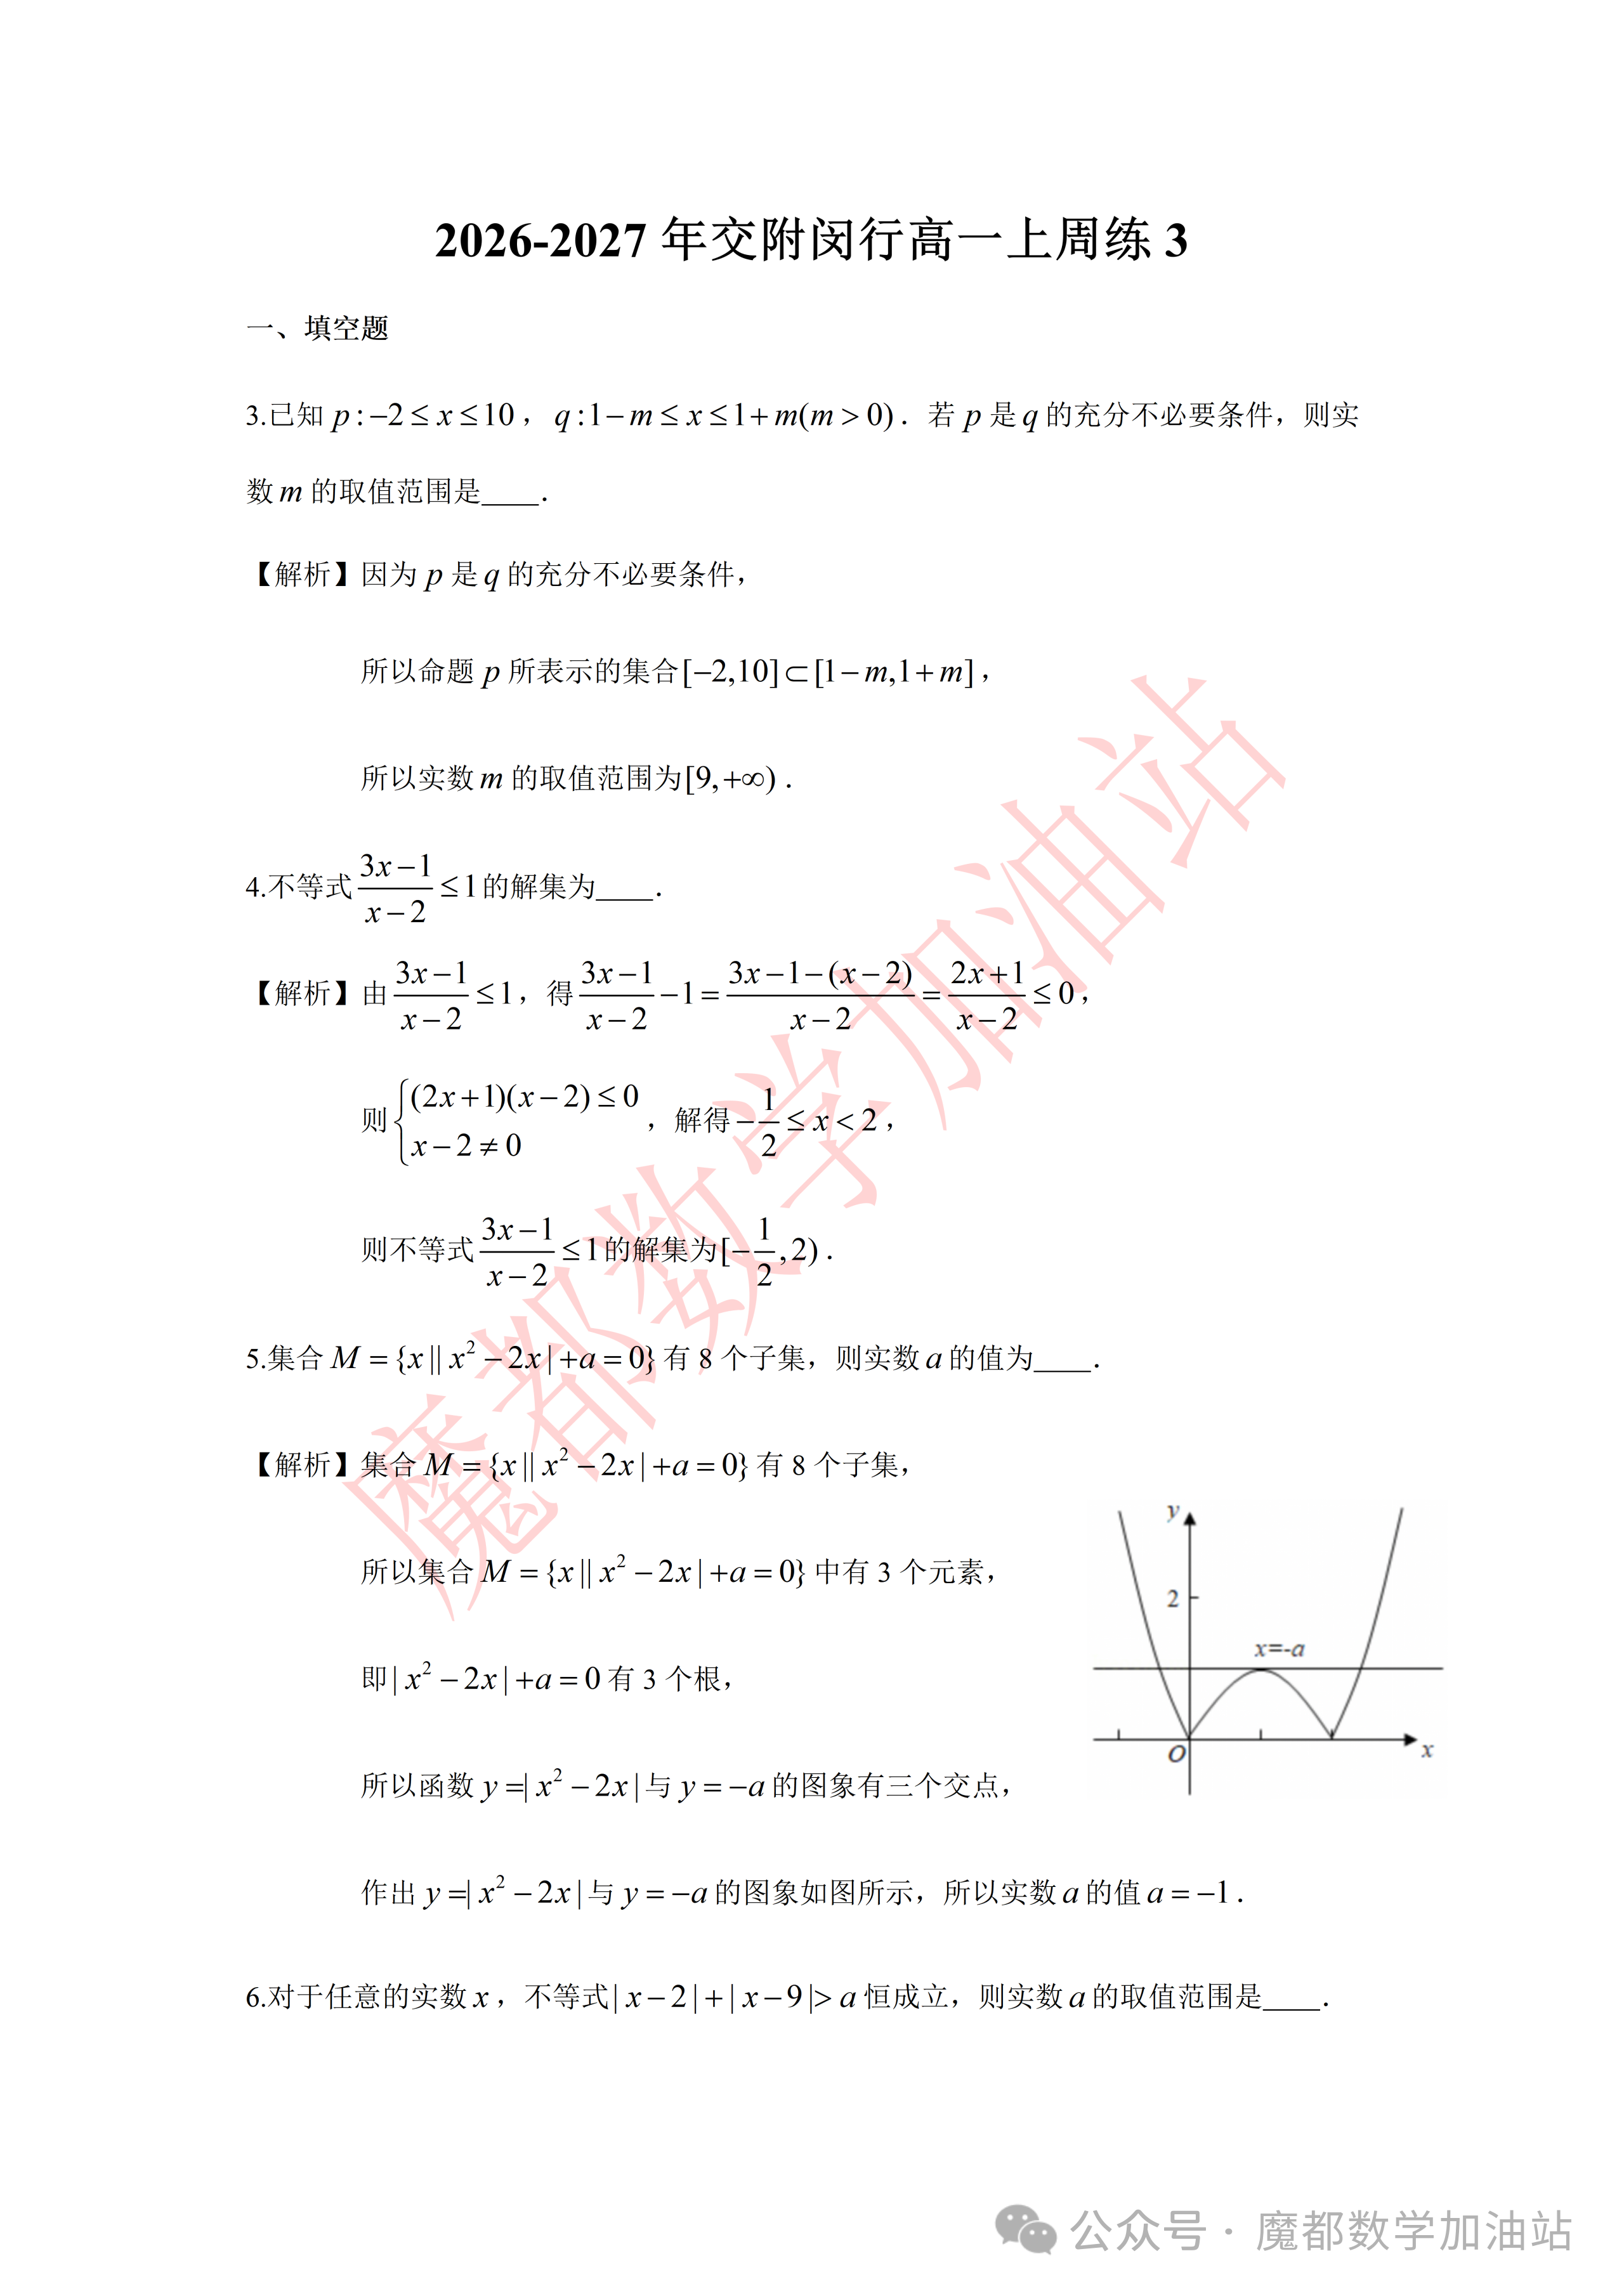
\includegraphics[width=0.14\textwidth,trim={1721bp 837bp 280bp 2297bp},clip]{../原图/高一43_交附闵行_周练3/01.png}
\end{center}

\solbegin
\step{集合 $M=\{x\mid |x^2-2x|+a=0\}$ 有 8 个子集，}
\step{所以集合 $M=\{x\mid |x^2-2x|+a=0\}$ 中有 3 个元素，}
\step{即 $|x^2-2x|+a=0$ 有 3 个根，}
\step{所以函数 $y=|x^2-2x|$ 与 $y=-a$ 的图象有三个交点，}
\step{作出 $y=|x^2-2x|$ 与 $y=-a$ 的图象如图所示，所以实数 $a$ 的值 $a=-1$.}
\solend

\fi

\item 对于任意的实数 $x$，不等式 $|x-2|+|x-9|>a$ 恒成立，则实数 $a$ 的取值范围是 \blankline[4.4em].

\ifanswer
\solbegin
\step{由绝对值的几何意义得 $|x-2|+|x-9|\geqslant7$，当且仅当 $2\leqslant x\leqslant9$ 时等号成立，}
\step{所以 $a<7$，}
\step{即 $a$ 的取值范围为 $(-\infty,7)$.}
\solend

\fi

\item 已知集合 $A=\{x\mid(a-1)x^2+3x-2=0\}$，$B=\{x\mid x^2-3x+2=0\}$，$A\subseteq B$，求实数 $a$ 的取值范围是 \blankline[4.4em].

\ifanswer
\solbegin
\step{由方程 $x^2-3x+2=0$，解得 $x=1$ 或 $x=2$，即 $B=\{1,2\}$，}
\step{因为 $A\subseteq B$，所以 $A=\varnothing$ 或 $A=\{1\}$ 或 $A=\{2\}$ 或 $A=\{1,2\}$，}
\step{当 $A=\varnothing$ 时，$a\neq1$，且 $\Delta=3^2-4(a-1)\times(-2)<0$，解得 $a<-\dfrac18$，}
\step{将 $x=1$ 代入方程 $(a-1)x^2+3x-2=0$，得 $a=0$，}
\step{此时 $A=\{x\mid-x^2+3x-2=0\}=\{1,2\}$，满足条件，}
\step{将 $x=2$ 代入方程 $(a-1)x^2+3x-2=0$，得到 $a=0$，上面已经验证满足条件，}
\step{综上所述，$a$ 的取值范围是 $\left(-\infty,-\dfrac18\right)\cup\{0\}$.}
\solend

\fi

\item 已知 $a$、$b$、$c$、$d$ 为常数，若不等式
$\dfrac{b}{x+a}+\dfrac{x+d}{x+c}<0$ 的解集为 $\left(-1,-\dfrac13\right)\cup\left(\dfrac12,1\right)$，
则不等式 $\dfrac{bx}{ax-1}+\dfrac{dx-1}{cx-1}<0$ 的解集为 \blankline[4.4em].

\ifanswer
\solbegin
\step{若 $x=0$，原不等式化为 $1<0$，不等式显然不成立，所以 $x\neq0$，}
\step{由 $\dfrac{bx}{ax-1}+\dfrac{dx-1}{cx-1}<0$，得 $\dfrac{b}{a-\dfrac1x}+\dfrac{d-\dfrac1x}{c-\dfrac1x}<0$，即 $\dfrac{b}{-\dfrac1x+a}+\dfrac{-\dfrac1x+d}{-\dfrac1x+c}<0$.}
\step{因为不等式 $\dfrac{b}{x+a}+\dfrac{x+d}{x+c}<0$ 的解集为 $\left(-1,-\dfrac13\right)\cup\left(\dfrac12,1\right)$，}
\step{所以 $-1<-\dfrac1x<-\dfrac13$ 或 $\dfrac12<-\dfrac1x<1$，解得 $1<x<3$ 或 $-2<x<-1$，}
\step{所以不等式 $\dfrac{bx}{ax-1}+\dfrac{dx-1}{cx-1}<0$ 的解集为 $(-2,-1)\cup(1,3)$.}
\solend

\fi

\item 正实数 $x$、$y$ 满足 $2x+3y-xy=0$，且存在这样的 $x$、$y$ 使不等式 $x+y<m+1$ 有解，则实数 $m$ 的取值范围是 \blankline[4.4em].

\ifanswer
\solbegin
\step{因为正实数 $x$、$y$ 满足 $2x+3y-xy=0$，则 $\dfrac2y+\dfrac3x=1$，$x>0$，$y>0$，}
\step{所以 $x+y=(x+y)\left(\dfrac3x+\dfrac2y\right)=3+\dfrac{2x}{y}+\dfrac{3y}{x}+2\geqslant2\sqrt{\dfrac{2x}{y}\times\dfrac{3y}{x}}+5=5+2\sqrt6$，}
\step{当且仅当 $\sqrt2x=\sqrt3y$ 时取等号，}
\step{存在这样的 $x$、$y$ 使不等式 $x+y<m+1$ 有解，则 $m+1>5+2\sqrt6$，}
\step{则 $m>4+2\sqrt6$，所以实数 $m$ 的取值范围是 $(4+2\sqrt6,+\infty)$.}
\solend

\fi

\item 若 $a$、$b$、$c\in\R$，$a^2+b^2+c^2=1$，则 $2ab+bc$ 的最大值为 \blankline[4.4em].

\ifanswer
\solbegin
\step{对于 $2ab+bc$，将 $b^2$ 拆分为 $\dfrac45b^2+\dfrac15b^2$，则 $a^2+\dfrac45b^2+c^2+\dfrac15b^2=1$，}
\step{$a^2+\dfrac45b^2\geqslant2\cdot a\cdot\dfrac2{\sqrt5}b=\dfrac4{\sqrt5}ab$，$c^2+\dfrac15b^2\geqslant2\cdot c\cdot\dfrac1{\sqrt5}b=\dfrac2{\sqrt5}bc$，}
\step{两式相加得 $1\geqslant\dfrac4{\sqrt5}ab+\dfrac2{\sqrt5}bc=\dfrac2{\sqrt5}(2ab+bc)$，故 $2ab+bc\leqslant\dfrac{\sqrt5}2$，}
\step{等号成立当且仅当 $a=\dfrac2{\sqrt5}b$，$c=\dfrac1{\sqrt5}b$，}
\step{代入 $a^2+b^2+c^2=1$，得 $\dfrac45b^2+b^2+\dfrac15b^2=2b^2=1$，即 $b=\dfrac{\sqrt2}2$，}
\step{此时 $a=\dfrac{\sqrt{10}}5$，$c=\dfrac{\sqrt{10}}{10}$，故 $2ab+bc$ 的最大值为 $\dfrac{\sqrt5}2$.}
\solend

\fi

\item 已知实数 $a$、$b$ 满足 $-3<a+2b<2$，$-1<2a-b<4$，则 $a+b$ 的取值范围为 \blankline[4.4em].

\ifanswer
\solbegin
\step{设 $a+b=m(a+2b)+n(2a-b)=(m+2n)a+(2m-n)b$，}
\step{所以 $\begin{cases}m+2n=1\\2m-n=1\end{cases}$，解得 $n=\dfrac15$，$m=\dfrac35$，所以 $a+b=\dfrac35(a+2b)+\dfrac15(2a-b)$，}
\step{因为 $-3<a+2b<2$，$-1<2a-b<4$，}
\step{所以 $-\dfrac95<\dfrac35(a+2b)<\dfrac65$，$-\dfrac15<\dfrac15(2a-b)<\dfrac45$，}
\step{相加得 $-2<\dfrac35(a+2b)+\dfrac15(2a-b)<2$，即 $-2<a+b<2$，}
\step{故 $a+b$ 的取值范围为 $(-2,2)$.}
\solend

\fi

% 注：原卷题干与解析均印作 \sqrt{2xyz}，但按其自身答案 8 与取等值（$y=\dfrac12$，
% $x=\dfrac{\sqrt3}4$，$z=\dfrac{\sqrt6}4$）代入只与 $\sqrt{2x^2y^2z^2}=\sqrt2\,xyz$ 相符，
% $\sqrt{2xyz}$ 与答案 8 不自洽，原卷如此，照录未改。
\item 已知正数 $x$、$y$、$z$ 满足 $2x^2+y^2+z^2=1$，则 $\dfrac{y+1}{\sqrt{2xyz}}$ 的最小值为 \blankline[4.4em].

\ifanswer
\solbegin
\step{由条件得 $2x^2+z^2=1-y^2=(1-y)(1+y)$，则 $1+y=\dfrac{2x^2+z^2}{1-y}$，}
\step{结合 $x$、$y$、$z>0$ 得原式 $=\dfrac{2x^2+z^2}{\sqrt{2xyz}(1-y)}\geqslant\dfrac{2\sqrt2xz}{\sqrt{2xyz}(1-y)}=\dfrac2{y(1-y)}$，}
\step{又 $y(1-y)\leqslant\left(\dfrac{y+1-y}2\right)^2=\dfrac14$，所以 $\dfrac2{y(1-y)}\geqslant\dfrac2{\frac14}=8$，}
\step{当且仅当 $\sqrt2x=z$，且 $y=1-y$，即 $y=\dfrac12$，$x=\dfrac{\sqrt3}4$，$z=\dfrac{\sqrt6}4$ 时取等号，}
\step{故 $\dfrac{y+1}{\sqrt{2xyz}}$ 最小值为 $8$.}
\solend

\fi

\end{enumerate}

\bigsec{二、选择题}

\begin{enumerate}
\setcounter{enumi}{12}

\item 已知关于 $x$ 的方程 $(1-k)x^2-2x-1=0$ 有实数根，则 $k$ 的取值范围是\mbox{（\quad）}

\keepwithprev
A. $k\leqslant2$ 且 $k\neq1$\qquad B. $k\leqslant2$\qquad
C. $k<2$ 且 $k\neq1$\qquad D. $k<2$

\ans{$A$}

\ifanswer
\solbegin
\step{由题意得 $\begin{cases}1-k\neq0\\\Delta=4+4(1-k)\geqslant0\end{cases}$，解不等式得 $\begin{cases}1\neq k\\2-k>0\end{cases}$，所以 $k\leqslant2$ 且 $k\neq1$，}
\step{故选 $A$.}
\solend

\fi

\item 不等式 $2|x+2|+|x-1|\geqslant5$ 成立的一个必要不充分条件是\mbox{（\quad）}

\keepwithprev
A. $x\leqslant-1$ 或 $x\geqslant0$\qquad B. $x\geqslant0$

C. $x\leqslant-\dfrac83$ 或 $x\geqslant0$\qquad D. $x\geqslant1$

\ans{$A$}

\ifanswer
\solbegin
\step{当 $x<-2$ 时，原不等式可化为 $-2x-4-x+1\geqslant5$，解得 $x\leqslant-\dfrac83$，}
\step{当 $-2\leqslant x<1$ 时，原不等式可化为 $2x+4-x+1\geqslant5$，解得 $0\leqslant x<1$，}
\step{当 $x\geqslant1$ 时，原不等式可化为 $2x+4+x-1\geqslant5$，解得 $x\geqslant\dfrac23$，得 $x\geqslant1$，}
\step{综上所述，不等式 $2|x+2|+|x-1|\geqslant5$ 成立的充要条件是 $x\leqslant-\dfrac83$ 或 $x\geqslant0$，}
\step{设 $A=\{x\mid x\leqslant-\dfrac83\text{ 或 }x\geqslant0\}$，}
\step{则不等式 $2|x+2|+|x-1|\geqslant5$ 成立的必要不充分条件，}
\step{其对应的集合 $B$ 满足 $A\subsetneq B$，对照各个选项，$A$ 项符合题意. 故选 $A$.}
\solend

\fi

\item 已知实数 $a>0$，$b>0$，$\dfrac1{a+1}+\dfrac1{b+1}=1$，则 $2a+3b$ 的最小值为\mbox{（\quad）}

\keepwithprev
A. $2\sqrt6$\qquad B. $3+2\sqrt6$\qquad
C. $5+2\sqrt6$\qquad D. $3+2\sqrt2$

\ans{$A$}

\ifanswer
\solbegin
\step{因为 $a>0$，$b>0$，$\dfrac1{a+1}+\dfrac1{b+1}=1$，}
\step{所以 $2a+3b=2(a+1)+3(b+1)-5=[2(a+1)+3(b+1)]\cdot\left(\dfrac1{a+1}+\dfrac1{b+1}\right)-5$}
\step{$=\left[2+3+\dfrac{3(b+1)}{a+1}+\dfrac{2(a+1)}{b+1}\right]-5\geqslant5+2\sqrt{\dfrac{3(b+1)}{a+1}\times\dfrac{2(a+1)}{b+1}}-5=2\sqrt6$，}
\step{当且仅当 $\dfrac{3(b+1)}{a+1}=\dfrac{2(a+1)}{b+1}$，即 $a=\dfrac{\sqrt6}2$，$b=\dfrac{\sqrt6}3$ 时取等号. 故选 $A$.}
\solend

\fi

\item 已知集合 $U=\{n\mid1\leqslant n\leqslant2027,\ n\in\N\}$，集合 $M\subseteq U$，若对于 $M$ 中任意两个不同的元素 $x$ 和 $y$，都有 $|x-y|>2$，则 $M$ 中元素个数的最大值是\mbox{（\quad）}

\keepwithprev
A. $676$\qquad B. $675$\qquad C. $672$\qquad D. $671$

\ans{$A$}

\ifanswer
\solbegin
\step{对于 $M$ 中的任意两个不同的元素 $x$、$y$，都有 $|x-y|>2$，}
\step{不妨设 $x>y$，都有 $x-y\geqslant3$，}
\step{要想 $M$ 所含元素个数最大，则要 $x-y$ 尽可能小，故需使得 $x-y$ 的最小值为 3，}
\step{将 $1\sim2027$ 这 2027 个元素按如下分组：}
\step{$\{1,2,3\}$，$\{4,5,6\}$，$\cdots$，$\{2023,2024,2025\}$，$\{2026,2027\}$，}
\step{故应在前 675 组中按周期 3 每组取一个元素，且第一组中不能取 3，}
\step{第一组中取 1 时，得 $M=\{1,4,7,\cdots,2023,2026\}$，}
\step{或 $M=\{1,4,7,\cdots,2023,2027\}$ 这样的集合，}
\step{第一组取 2 时，得 $M=\{2,5,8,\cdots,2024,2027\}$，}
\step{其中任意两元素差值 $x-y$（$x>y$）都大于 2，满足题意，}
\step{故 $M$ 所含元素个数的最大值为 $\dfrac{2025}{3}+1=676$. 故选 $A$.}
\solend

\fi

\end{enumerate}

\bigsec{三、解答题}

\begin{enumerate}
\setcounter{enumi}{16}

\item 已知 $a\in\R$，集合 $A=\left\{x\middle|\dfrac{2-x}{x+1}\leqslant0\right\}$，$B=\{x\mid x^2+(3-a)x-3a<0\}$.

\begin{enumerate}[label=(\arabic*)]
\item 当 $a=\dfrac13$ 时，求 $A$ 和 $B$；
\item 已知 $A\cup B=A$，求实数 $a$ 的取值范围.
\end{enumerate}

\ifanswer
\solbegin
\stepm{(1)}{由 $\dfrac{2-x}{x+1}\leqslant0$，得 $\begin{cases}(2-x)(x+1)\leqslant0\\x\neq-1\end{cases}$，解得 $x<-1$ 或 $x\geqslant2$，}
\step{则 $A=\{x\mid x<-1\text{ 或 }x\geqslant2\}$；}
\step{$B=\{x\mid x^2+(3-a)x-3a<0\}=\{x\mid(x+3)(x-a)<0\}$，}
% 注：原卷此行印作 $(x+2)\left(x-\dfrac13\right)$，按前一行 $B=\{x\mid(x+3)(x-a)<0\}$ 应为
% $(x+3)\left(x-\dfrac13\right)$，原卷如此，照录未改。
\step{当 $a=\dfrac13$ 时，$B=\left\{x\middle|(x+2)\left(x-\dfrac13\right)<0\right\}$，}
\step{解得 $B=\left\{x\middle|-3<x<\dfrac13\right\}$.}
\stepm{(2)}{由 $A\cup B=A$，得 $B\subseteq A$，}
\step{①当 $B=\varnothing$ 时，得 $a=-3$，符合题意；}
\step{②当 $B\neq\varnothing$ 时，若 $a>-3$，则 $B=\{x\mid-3<x<a\}$，}
\step{由 $B\subseteq A$，得 $a\leqslant-1$，此时 $-3<a\leqslant-1$；}
\step{若 $a<-3$，则 $B=\{x\mid a<x<-3\}$，此时 $B\subseteq A$ 恒成立，}
\step{故 $a<-3$ 符合题意；}
\step{综上所述，实数 $a$ 的取值范围为 $a\leqslant-1$.}
\solend

\fi

\ansspace[6]

\item 甲乙两地的高速公路全长 166 千米，汽车从甲地进入该高速公路后匀速行驶到乙地，车速 $v\in[70,120]$（千米/时）. 已知汽车每小时的运输成本（以元为单位）由可变部分和固定部分组成：可变部分为 $0.02v^2$，固定部分为 220 元.

\begin{enumerate}[label=(\arabic*)]
\item 若每小时的运输成本不高于 420 元，汽车的速度应该控制在什么范围？
\item 汽车应以多大速度行驶才能使全程运输成本最小？最小运输成本约为多少元？（结果保留整数）
\end{enumerate}

\ifanswer
\solbegin
\stepm{(1)}{已知汽车每小时的运输成本（以元为单位）由可变部分和固定部分组成：}
\step{可变部分为 $0.02v^2$，固定部分为 220 元，}
\step{则汽车每小时的运输成本为 $0.02v^2+220$（元），}
\step{若每小时的运输成本不高于 420 元，}
\step{则 $0.02v^2+220\leqslant420$，解得 $v^2\leqslant10000$，}
\step{得 $70\leqslant v\leqslant100$，即 $v\in[70,100]$（千米/时），}
\step{则此时汽车的速度 $v$ 应该控制在 $[70,100]$（千米/时）；}
\stepm{(2)}{因为汽车从甲地进入该高速公路后匀速行驶到乙地，}
\step{车速 $v\in[70,120]$（千米/时），所以汽车的行驶时间为 $\dfrac{166}{v}$（小时），}
\step{所以全程运输成本 $y=\dfrac{166}{v}(0.02v^2+220)=3.32v+\dfrac{36520}{v}$，}
% 注：原卷此行印作 $v\in[70,100]$，与题干的 $v\in[70,120]$ 不自洽（若 $v\in[70,100]$，
% 最小值应在 $v=100$ 处取得，与下文 $v=10\sqrt{110}\approx105$ 矛盾），原卷如此，照录未改。
\step{$v\in[70,100]$，}
\step{由基本不等式得 $y=3.32v+\dfrac{36520}{v}\geqslant2\sqrt{3.32v\times\dfrac{36520}{v}}\approx696$，}
\step{当且仅当 $3.32v=\dfrac{36520}{v}$，即 $v=10\sqrt{110}\approx105$ 时取等号，}
\step{汽车应以 105（千米/时）行驶才能使全程运输成本最小，}
\step{最小运输成本约为 696 元.}
\solend

\fi

\ansspace[8]

\item
\begin{enumerate}[label=(\arabic*)]
\item 已知 $a$、$b$、$c$ 为实数，求证：$|a-b|\leqslant|a-c|+|b-c|$，并说明等号成立的条件；
\item 设 $x\in\R$，求方程 $|3x-8|=|5-x|+|2x-3|$ 的解集.
\end{enumerate}

\ifanswer
% 注：原卷第 19 题未印【解析】，仅印一行【答案】"（1）(a-c)(b-c)≤0；
% （2）(-∞,3/2]∪[5,+∞)"。(1) 的两行推导为本稿所补，(2) 照录原卷答案。
% 又题干作"方程"，而所给答案 (-∞,3/2]∪[5,+∞) 实为不等式 |3x-8|≤|5-x|+|2x-3| 的解集，
% 与"方程"不合，原卷如此，照录未改。
\solbegin
\stepm{(1)}{由三角不等式 $|a-b|=|(a-c)-(b-c)|\leqslant|a-c|+|b-c|$，}
\step{当且仅当 $(a-c)(b-c)\leqslant0$ 时等号成立.}
\stepm{(2)}{$\left(-\infty,\dfrac32\right]\cup[5,+\infty)$.}
\solend

\fi

\ansspace[6]

\item 已知正实数 $a$、$b$ 满足 $a+b=1$，求 $\dfrac1a+\dfrac1b$ 的最小值. 其中一种解法是：

\[
\begin{aligned}
\dfrac1a+\dfrac1b
&=\left(\dfrac1a+\dfrac1b\right)(a+b)\\
&=1+\dfrac ba+\dfrac ab+1\\
&\geqslant2+2\sqrt{\dfrac ba\times\dfrac ab}=2+2=4.
\end{aligned}
\]
当且仅当 $\dfrac ba=\dfrac ab$ 且 $a+b=1$ 时即 $a=b=\dfrac12$ 时取等号.
学习上述解法并解决下列问题：

\begin{enumerate}[label=(\arabic*)]
\item 若正实数 $x$、$y$ 满足 $x+y=xy$，求 $2x+y$ 的最小值；
\item 若实数 $a$、$b$、$x$、$y$ 满足 $\dfrac{x^2}{a^2}+\dfrac{y^2}{b^2}=1$，求证：$a^2+b^2\geqslant(x+y)^2$；
\item 求代数式 $M=\sqrt{m-1}+\sqrt{3-m}$ 的最大值，并求出使得 $M$ 最大的 $m$ 的值.
\end{enumerate}

\ifanswer
\solbegin
\stepm{(1)}{因为正实数 $x$、$y$ 满足 $x+y=xy$，$\dfrac{x+y}{xy}=1\Rightarrow\dfrac1y+\dfrac1x=1$，}
\step{所以 $(2x+y)\times1=(2x+y)\left(\dfrac1y+\dfrac1x\right)=3+\dfrac{2x}{y}+\dfrac yx\geqslant3+2\sqrt{\dfrac{2x}{y}\cdot\dfrac yx}=3+2\sqrt2$，}
\step{当且仅当 $\dfrac{2x}{y}=\dfrac yx$ 且 $\dfrac1y+\dfrac1x=1$ 时取等号，}
\step{解得 $x=\dfrac{2+\sqrt2}2$，$y=\sqrt2x=\sqrt2\times\dfrac{2+\sqrt2}2=1+\sqrt2$，}
\step{所以 $2x+y$ 的最小值为 $3+2\sqrt2$；}
\stepm{(2)}{因为 $\dfrac{x^2}{a^2}+\dfrac{y^2}{b^2}=1$，}
\step{所以 $a^2+b^2=(a^2+b^2)\left(\dfrac{x^2}{a^2}+\dfrac{y^2}{b^2}\right)=x^2+y^2+\dfrac{b^2x^2}{a^2}+\dfrac{a^2y^2}{b^2}$，}
\step{因为 $\dfrac{b^2x^2}{a^2}+\dfrac{a^2y^2}{b^2}\geqslant2\sqrt{\dfrac{b^2x^2}{a^2}\times\dfrac{a^2y^2}{b^2}}=2\sqrt{x^2y^2}=2|xy|$，}
\step{当且仅当 $\dfrac{b^2x^2}{a^2}=\dfrac{a^2y^2}{b^2}$ 时取等号，}
\step{所以 $x^2+y^2+\dfrac{b^2x^2}{a^2}+\dfrac{a^2y^2}{b^2}\geqslant x^2+y^2+2|xy|\geqslant x^2+y^2+2xy=(x+y)^2$，}
\step{所以 $a^2+b^2\geqslant(x+y)^2$；}
\stepm{(3)}{因为 $M=\sqrt{m-1}+\sqrt{3-m}$，所以 $\begin{cases}m-1\geqslant0\\3-m\geqslant0\end{cases}$，解得 $1\leqslant m\leqslant3$，}
\step{所以 $M^2=(\sqrt{m-1}+\sqrt{3-m})^2=2+2\sqrt{(3-m)(m-1)}$，}
\step{由基本不等式得 $(3-m)(m-1)\leqslant\left(\dfrac{(3-m)+(m-1)}2\right)^2=1$，}
\step{当且仅当 $3-m=m-1$ 时取等号，解得 $m=2$，}
\step{所以 $M^2=2+2\sqrt{(3-m)(m-1)}\leqslant2+2\sqrt1=4$，}
\step{因为 $M>0$，所以 $M\leqslant2$，所以 $M$ 最大值为 2，此时 $m$ 的值为 2.}
\solend

\fi

\ansspace[8]

\item 若有限个正整数组成的集合 $A$ 中至少有两个元素，且对于任意的 $x,y\in A$（$x>y$），都有 $\dfrac{y^2}{x-y}\in A$，则称 $A$ 为“L-集合”.

\begin{enumerate}[label=(\arabic*)]
\item 判断 $\{1,2,4\}$ 是否为“L-集合”，说明理由；
\item 若双元素集 $M$ 为“L-集合”，且 $4\in M$，求所有满足条件的集合 $M$；
\item 求所有满足条件的“L-集合”.
\end{enumerate}

\ifanswer
\solbegin
\stepm{(1)}{若至少由两个元素构成的有限集合 $A\subseteq\N^*$，}
% 注：原卷下一行"都有"后未印分数 \dfrac{y^2}{x-y}，径作"都有 A"，原卷如此，照录未改。
\step{且对于任意的 $x$、$y\in A$（$x>y$），都有 $A$，则称 $A$ 为“L-集合”，}
\step{$\{1,2,4\}$ 不为“L-集合”，理由如下：}
\step{因为 $\dfrac{1^2}{4-1}=\dfrac13\notin\{1,2,4\}$，所以 $\{1,2,4\}$ 不是“L-集合”.}
\stepm{(2)}{设 $M=\{4,m\}$（$m\in\N^*$，$m\neq4$），}
\step{若 $m<4$，则 $\dfrac{m^2}{4-m}=m$ 或 $\dfrac{m^2}{4-m}=4$，}
\step{由 $\dfrac{m^2}{4-m}=m$，解得 $m=2$，$m=0$（舍去），此时 $M=\{2,4\}$；}
\step{由 $\dfrac{m^2}{4-m}=4$ 化为 $m^2+4m-16=0$，而 $\Delta=4^2+4\times16=80$，}
\step{故方程无正整数解.}
\step{若 $m>4$，则 $\dfrac{4^2}{m-4}=4$ 或 $\dfrac{4^2}{m-4}=m$，}
\step{由 $\dfrac{4^2}{m-4}=4$，解得 $m=8$，此时 $M=\{4,8\}$；}
\step{由 $\dfrac{4^2}{m-4}=m$ 化为 $m^2-4m-16=0$，而 $\Delta=4^2+4\times16=80$，}
\step{故方程无正整数解.}
\step{综上，双元素集 $M$ 为“L-集合”，且 $4\in M$，}
\step{则所有满足条件的集合 $M$ 为 $\{4,8\}$，$\{2,4\}$.}
\stepm{(3)}{若“L-集合”为双元素集，}
\step{不妨设 $M=\{k,m\}$（$k,m\in\N^*$，$m>k$），则 $\dfrac{k^2}{m-k}=k$ 或 $\dfrac{k^2}{m-k}=m$，}
\step{由 $\dfrac{k^2}{m-k}=k$，则 $2k^2=mk$，而 $m>k$，故 $m=2k$，此时 $M=\{k,2k\}$；}
\step{由 $\dfrac{k^2}{m-k}=m$，则 $m^2-mk-k^2=0$，而 $\Delta=5k^2$，显然不存在正整数解；}
\step{所以，“L-集合”为 $\{k,2k\}$，其中 $k\in\N^*$.}
\step{若“L-集合”含有两个以上的元素，}
\step{设最小的元素为 $b$，最大的元素为 $a$，第二大的元素为 $n$，}
\step{则 $\dfrac{b^2}{a-b}$，$\dfrac{n^2}{a-n}$ 是“L-集合”中的元素，}
% 注：原卷下一行未印"由于'L-集合'中的元素均为正整数"一语，径作"若 \dfrac{b^2}{a-b}\geqslant b"，
% 原卷如此，照录未改。
\step{若 $\dfrac{b^2}{a-b}\geqslant b$，解得 $a\leqslant2b$，}
\step{若 $\dfrac{n^2}{a-n}\leqslant n$，则 $a\geqslant2n>2b$，矛盾，}
\step{若 $\dfrac{n^2}{a-n}=a$，该方程的解为 $n=\dfrac{\sqrt5-1}2a$，则 $n$、$a$ 不可能同时为整数，}
\step{无解.}
\step{所以所有满足条件的“L-集合”为 $\{k,2k\}$，其中 $k\in\N^*$.}
\solend

\fi

\ansspace*[10]

\end{enumerate}

\end{document}
"
% 紧凑版：xelatex "\def\iscompact{1}% 高一43_交附闵行_周练3.tex
%   —— 高一上数学“2026-2027 年交附闵行高一上周练3”（试卷版/答案版）
% 试卷版：xelatex 高一43_交附闵行_周练3.tex
% 答案版：xelatex "\def\isanswer{1}\input{高一43_交附闵行_周练3.tex}"
% 紧凑版：xelatex "\def\iscompact{1}\input{高一43_交附闵行_周练3.tex}"
%
% 原始材料是微信公众号图文（公众号“魔都数学加油站”，作者破晓，2026-10-01 21:37，
% 原文标题“27学年高一43——2026-2027年上海市交附闵行高一上周练3”，
% https://mp.weixin.qq.com/s/-rgkOD9jJVpug6s0uSbwmQ）。正文为 12 张 PNG 页；
% 第 01、05、09、12 页 2560×3620，其余第 02—04、06—08、10—11 页 4762×6735。
% 原文本身是讲评版，题目下方印有解析/答案；题目与讲解照原卷转录，保留原卷错误。
%
% 卷首标题：原卷印作“2026-2027 年交附闵行高一上周练3”，公众号标题中的“上海市”
% 三字不在卷面标题中，本稿依卷面录入；年份区间按全稿惯例排 en dash。
%
% 与原卷的排版差异：
%   ① 原文从第 3 题开始（第 1、2 题未在这篇推文中发布），本稿保留原题号 3—21；
%   ② 原卷本就印有“一、填空题”“二、选择题”“三、解答题”，本稿照原卷分节，
%      改排为全稿统一的大节标题；
%   ③ 原卷未印副标题，本稿按“知识模块”口径补出“集合与常用逻辑用语、不等式”；
%   ④ 原卷填空横线依全稿惯例排为 \blankline[4.4em]；选择题答案只在答案版以 \ans{} 显示，
%      解答区以 \ifanswer 分离；解答题按原卷留出标准作答空间；
%   ⑤ 第 5 题图取自原卷第 1 页截图并裁入本稿，不另建图档；公众号水印不录入。
%      原卷图页分页不保留，正文依本稿版心重新分页。
%
% 原卷存疑/错误（均照录，未改）：
%   ① 第 9 题原卷题干即作"正实数 x、y"，与解析 x>0、y>0 相容，并无矛盾（初稿曾误记
%      题干只称"实数"并据此指原卷不自洽，2026-10-05 回原图核对订正）。
%   ② 第 11 题解析"相加得"一行原卷印作 -2<3/5(a+2b)+1/5(2a-b)<2，第一项系数 3/5
%      原卷不缺（初稿漏抄致该行按字面不成立，2026-10-05 已按原卷补回）。
%   ③ 第 13 题答案印 A，解析以“1-k≠0”排除 k=1；但 k=1 时原方程为 -2x-1=0，
%      仍有实数根，按题意应选 B。本稿保留原卷答案 A 及其解析，不代为订正。
%
\documentclass[a4paper,11pt]{article}
\usepackage{common}
\usepackage{graphicx}

\begin{document}

\examtitlest[3]{2026--2027 年交附闵行高一上周练 3}{集合与常用逻辑用语、不等式}

\bigsec{一、填空题}

\begin{enumerate}
\setcounter{enumi}{2}

\item 已知 $p\colon -2\leqslant x\leqslant10$，$q\colon 1-m\leqslant x\leqslant1+m$（$m>0$）. 若 $p$ 是 $q$ 的充分不必要条件，则实数 $m$ 的取值范围是 \blankline[4.4em].

\ifanswer
\solbegin
\step{因为 $p$ 是 $q$ 的充分不必要条件，}
\step{所以命题 $p$ 所表示的集合 $[-2,10]\subset[1-m,1+m]$，}
\step{所以实数 $m$ 的取值范围为 $[9,+\infty)$.}
\solend

\fi

\item 不等式 $\dfrac{3x-1}{x-2}\leqslant1$ 的解集为 \blankline[4.4em].

\ifanswer
\solbegin
\step{由 $\dfrac{3x-1}{x-2}-1=\dfrac{3x-1-(x-2)}{x-2}=\dfrac{2x+1}{x-2}\leqslant0$，}
\step{则 $\begin{cases}(2x+1)(x-2)\leqslant0\\x-2\neq0\end{cases}$，解得 $-\dfrac12\leqslant x<2$，}
\step{则不等式 $\dfrac{3x-1}{x-2}\leqslant1$ 的解集为 $\left[-\dfrac12,2\right)$.}
\solend

\fi

\item 集合 $M=\{x\mid |x^2-2x|+a=0\}$ 有 8 个子集，则实数 $a$ 的值为 \blankline[4.4em].

\ifanswer
\begin{center}
% 图取自原卷第 1 页；用原图裁切，未重绘。
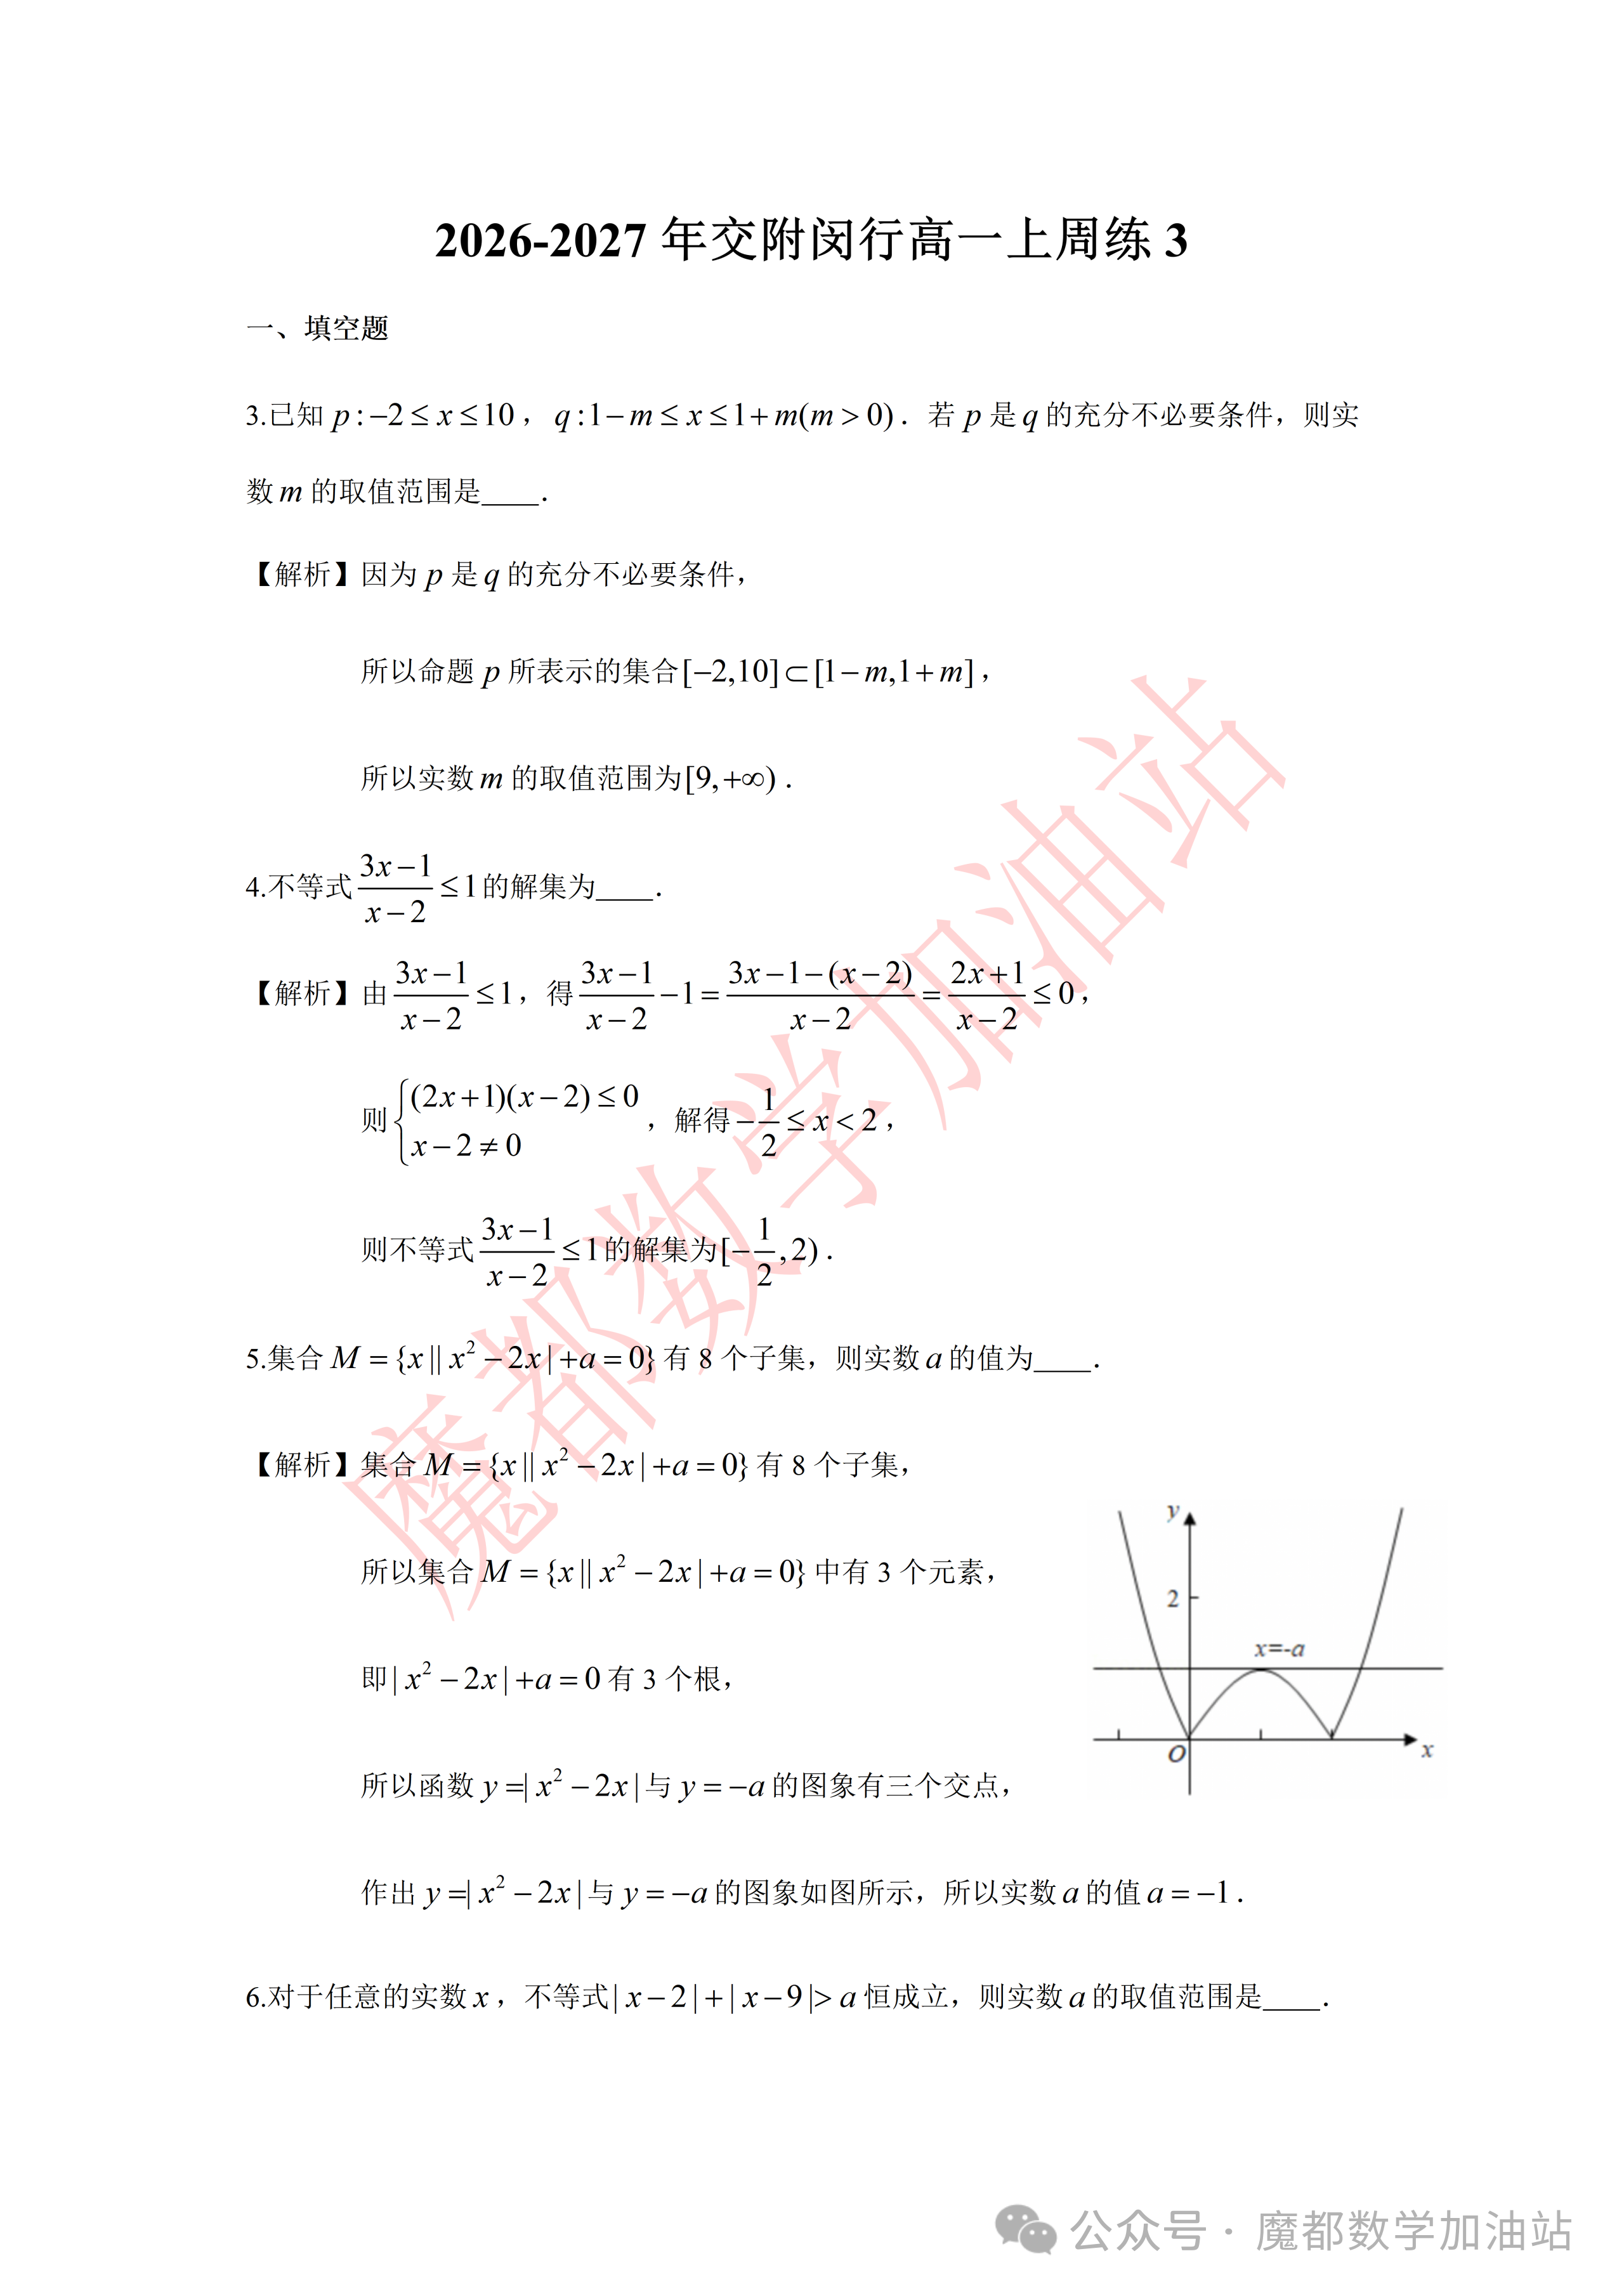
\includegraphics[width=0.14\textwidth,trim={1721bp 837bp 280bp 2297bp},clip]{../原图/高一43_交附闵行_周练3/01.png}
\end{center}

\solbegin
\step{集合 $M=\{x\mid |x^2-2x|+a=0\}$ 有 8 个子集，}
\step{所以集合 $M=\{x\mid |x^2-2x|+a=0\}$ 中有 3 个元素，}
\step{即 $|x^2-2x|+a=0$ 有 3 个根，}
\step{所以函数 $y=|x^2-2x|$ 与 $y=-a$ 的图象有三个交点，}
\step{作出 $y=|x^2-2x|$ 与 $y=-a$ 的图象如图所示，所以实数 $a$ 的值 $a=-1$.}
\solend

\fi

\item 对于任意的实数 $x$，不等式 $|x-2|+|x-9|>a$ 恒成立，则实数 $a$ 的取值范围是 \blankline[4.4em].

\ifanswer
\solbegin
\step{由绝对值的几何意义得 $|x-2|+|x-9|\geqslant7$，当且仅当 $2\leqslant x\leqslant9$ 时等号成立，}
\step{所以 $a<7$，}
\step{即 $a$ 的取值范围为 $(-\infty,7)$.}
\solend

\fi

\item 已知集合 $A=\{x\mid(a-1)x^2+3x-2=0\}$，$B=\{x\mid x^2-3x+2=0\}$，$A\subseteq B$，求实数 $a$ 的取值范围是 \blankline[4.4em].

\ifanswer
\solbegin
\step{由方程 $x^2-3x+2=0$，解得 $x=1$ 或 $x=2$，即 $B=\{1,2\}$，}
\step{因为 $A\subseteq B$，所以 $A=\varnothing$ 或 $A=\{1\}$ 或 $A=\{2\}$ 或 $A=\{1,2\}$，}
\step{当 $A=\varnothing$ 时，$a\neq1$，且 $\Delta=3^2-4(a-1)\times(-2)<0$，解得 $a<-\dfrac18$，}
\step{将 $x=1$ 代入方程 $(a-1)x^2+3x-2=0$，得 $a=0$，}
\step{此时 $A=\{x\mid-x^2+3x-2=0\}=\{1,2\}$，满足条件，}
\step{将 $x=2$ 代入方程 $(a-1)x^2+3x-2=0$，得到 $a=0$，上面已经验证满足条件，}
\step{综上所述，$a$ 的取值范围是 $\left(-\infty,-\dfrac18\right)\cup\{0\}$.}
\solend

\fi

\item 已知 $a$、$b$、$c$、$d$ 为常数，若不等式
$\dfrac{b}{x+a}+\dfrac{x+d}{x+c}<0$ 的解集为 $\left(-1,-\dfrac13\right)\cup\left(\dfrac12,1\right)$，
则不等式 $\dfrac{bx}{ax-1}+\dfrac{dx-1}{cx-1}<0$ 的解集为 \blankline[4.4em].

\ifanswer
\solbegin
\step{若 $x=0$，原不等式化为 $1<0$，不等式显然不成立，所以 $x\neq0$，}
\step{由 $\dfrac{bx}{ax-1}+\dfrac{dx-1}{cx-1}<0$，得 $\dfrac{b}{a-\dfrac1x}+\dfrac{d-\dfrac1x}{c-\dfrac1x}<0$，即 $\dfrac{b}{-\dfrac1x+a}+\dfrac{-\dfrac1x+d}{-\dfrac1x+c}<0$.}
\step{因为不等式 $\dfrac{b}{x+a}+\dfrac{x+d}{x+c}<0$ 的解集为 $\left(-1,-\dfrac13\right)\cup\left(\dfrac12,1\right)$，}
\step{所以 $-1<-\dfrac1x<-\dfrac13$ 或 $\dfrac12<-\dfrac1x<1$，解得 $1<x<3$ 或 $-2<x<-1$，}
\step{所以不等式 $\dfrac{bx}{ax-1}+\dfrac{dx-1}{cx-1}<0$ 的解集为 $(-2,-1)\cup(1,3)$.}
\solend

\fi

\item 正实数 $x$、$y$ 满足 $2x+3y-xy=0$，且存在这样的 $x$、$y$ 使不等式 $x+y<m+1$ 有解，则实数 $m$ 的取值范围是 \blankline[4.4em].

\ifanswer
\solbegin
\step{因为正实数 $x$、$y$ 满足 $2x+3y-xy=0$，则 $\dfrac2y+\dfrac3x=1$，$x>0$，$y>0$，}
\step{所以 $x+y=(x+y)\left(\dfrac3x+\dfrac2y\right)=3+\dfrac{2x}{y}+\dfrac{3y}{x}+2\geqslant2\sqrt{\dfrac{2x}{y}\times\dfrac{3y}{x}}+5=5+2\sqrt6$，}
\step{当且仅当 $\sqrt2x=\sqrt3y$ 时取等号，}
\step{存在这样的 $x$、$y$ 使不等式 $x+y<m+1$ 有解，则 $m+1>5+2\sqrt6$，}
\step{则 $m>4+2\sqrt6$，所以实数 $m$ 的取值范围是 $(4+2\sqrt6,+\infty)$.}
\solend

\fi

\item 若 $a$、$b$、$c\in\R$，$a^2+b^2+c^2=1$，则 $2ab+bc$ 的最大值为 \blankline[4.4em].

\ifanswer
\solbegin
\step{对于 $2ab+bc$，将 $b^2$ 拆分为 $\dfrac45b^2+\dfrac15b^2$，则 $a^2+\dfrac45b^2+c^2+\dfrac15b^2=1$，}
\step{$a^2+\dfrac45b^2\geqslant2\cdot a\cdot\dfrac2{\sqrt5}b=\dfrac4{\sqrt5}ab$，$c^2+\dfrac15b^2\geqslant2\cdot c\cdot\dfrac1{\sqrt5}b=\dfrac2{\sqrt5}bc$，}
\step{两式相加得 $1\geqslant\dfrac4{\sqrt5}ab+\dfrac2{\sqrt5}bc=\dfrac2{\sqrt5}(2ab+bc)$，故 $2ab+bc\leqslant\dfrac{\sqrt5}2$，}
\step{等号成立当且仅当 $a=\dfrac2{\sqrt5}b$，$c=\dfrac1{\sqrt5}b$，}
\step{代入 $a^2+b^2+c^2=1$，得 $\dfrac45b^2+b^2+\dfrac15b^2=2b^2=1$，即 $b=\dfrac{\sqrt2}2$，}
\step{此时 $a=\dfrac{\sqrt{10}}5$，$c=\dfrac{\sqrt{10}}{10}$，故 $2ab+bc$ 的最大值为 $\dfrac{\sqrt5}2$.}
\solend

\fi

\item 已知实数 $a$、$b$ 满足 $-3<a+2b<2$，$-1<2a-b<4$，则 $a+b$ 的取值范围为 \blankline[4.4em].

\ifanswer
\solbegin
\step{设 $a+b=m(a+2b)+n(2a-b)=(m+2n)a+(2m-n)b$，}
\step{所以 $\begin{cases}m+2n=1\\2m-n=1\end{cases}$，解得 $n=\dfrac15$，$m=\dfrac35$，所以 $a+b=\dfrac35(a+2b)+\dfrac15(2a-b)$，}
\step{因为 $-3<a+2b<2$，$-1<2a-b<4$，}
\step{所以 $-\dfrac95<\dfrac35(a+2b)<\dfrac65$，$-\dfrac15<\dfrac15(2a-b)<\dfrac45$，}
\step{相加得 $-2<\dfrac35(a+2b)+\dfrac15(2a-b)<2$，即 $-2<a+b<2$，}
\step{故 $a+b$ 的取值范围为 $(-2,2)$.}
\solend

\fi

% 注：原卷题干与解析均印作 \sqrt{2xyz}，但按其自身答案 8 与取等值（$y=\dfrac12$，
% $x=\dfrac{\sqrt3}4$，$z=\dfrac{\sqrt6}4$）代入只与 $\sqrt{2x^2y^2z^2}=\sqrt2\,xyz$ 相符，
% $\sqrt{2xyz}$ 与答案 8 不自洽，原卷如此，照录未改。
\item 已知正数 $x$、$y$、$z$ 满足 $2x^2+y^2+z^2=1$，则 $\dfrac{y+1}{\sqrt{2xyz}}$ 的最小值为 \blankline[4.4em].

\ifanswer
\solbegin
\step{由条件得 $2x^2+z^2=1-y^2=(1-y)(1+y)$，则 $1+y=\dfrac{2x^2+z^2}{1-y}$，}
\step{结合 $x$、$y$、$z>0$ 得原式 $=\dfrac{2x^2+z^2}{\sqrt{2xyz}(1-y)}\geqslant\dfrac{2\sqrt2xz}{\sqrt{2xyz}(1-y)}=\dfrac2{y(1-y)}$，}
\step{又 $y(1-y)\leqslant\left(\dfrac{y+1-y}2\right)^2=\dfrac14$，所以 $\dfrac2{y(1-y)}\geqslant\dfrac2{\frac14}=8$，}
\step{当且仅当 $\sqrt2x=z$，且 $y=1-y$，即 $y=\dfrac12$，$x=\dfrac{\sqrt3}4$，$z=\dfrac{\sqrt6}4$ 时取等号，}
\step{故 $\dfrac{y+1}{\sqrt{2xyz}}$ 最小值为 $8$.}
\solend

\fi

\end{enumerate}

\bigsec{二、选择题}

\begin{enumerate}
\setcounter{enumi}{12}

\item 已知关于 $x$ 的方程 $(1-k)x^2-2x-1=0$ 有实数根，则 $k$ 的取值范围是\mbox{（\quad）}

\keepwithprev
A. $k\leqslant2$ 且 $k\neq1$\qquad B. $k\leqslant2$\qquad
C. $k<2$ 且 $k\neq1$\qquad D. $k<2$

\ans{$A$}

\ifanswer
\solbegin
\step{由题意得 $\begin{cases}1-k\neq0\\\Delta=4+4(1-k)\geqslant0\end{cases}$，解不等式得 $\begin{cases}1\neq k\\2-k>0\end{cases}$，所以 $k\leqslant2$ 且 $k\neq1$，}
\step{故选 $A$.}
\solend

\fi

\item 不等式 $2|x+2|+|x-1|\geqslant5$ 成立的一个必要不充分条件是\mbox{（\quad）}

\keepwithprev
A. $x\leqslant-1$ 或 $x\geqslant0$\qquad B. $x\geqslant0$

C. $x\leqslant-\dfrac83$ 或 $x\geqslant0$\qquad D. $x\geqslant1$

\ans{$A$}

\ifanswer
\solbegin
\step{当 $x<-2$ 时，原不等式可化为 $-2x-4-x+1\geqslant5$，解得 $x\leqslant-\dfrac83$，}
\step{当 $-2\leqslant x<1$ 时，原不等式可化为 $2x+4-x+1\geqslant5$，解得 $0\leqslant x<1$，}
\step{当 $x\geqslant1$ 时，原不等式可化为 $2x+4+x-1\geqslant5$，解得 $x\geqslant\dfrac23$，得 $x\geqslant1$，}
\step{综上所述，不等式 $2|x+2|+|x-1|\geqslant5$ 成立的充要条件是 $x\leqslant-\dfrac83$ 或 $x\geqslant0$，}
\step{设 $A=\{x\mid x\leqslant-\dfrac83\text{ 或 }x\geqslant0\}$，}
\step{则不等式 $2|x+2|+|x-1|\geqslant5$ 成立的必要不充分条件，}
\step{其对应的集合 $B$ 满足 $A\subsetneq B$，对照各个选项，$A$ 项符合题意. 故选 $A$.}
\solend

\fi

\item 已知实数 $a>0$，$b>0$，$\dfrac1{a+1}+\dfrac1{b+1}=1$，则 $2a+3b$ 的最小值为\mbox{（\quad）}

\keepwithprev
A. $2\sqrt6$\qquad B. $3+2\sqrt6$\qquad
C. $5+2\sqrt6$\qquad D. $3+2\sqrt2$

\ans{$A$}

\ifanswer
\solbegin
\step{因为 $a>0$，$b>0$，$\dfrac1{a+1}+\dfrac1{b+1}=1$，}
\step{所以 $2a+3b=2(a+1)+3(b+1)-5=[2(a+1)+3(b+1)]\cdot\left(\dfrac1{a+1}+\dfrac1{b+1}\right)-5$}
\step{$=\left[2+3+\dfrac{3(b+1)}{a+1}+\dfrac{2(a+1)}{b+1}\right]-5\geqslant5+2\sqrt{\dfrac{3(b+1)}{a+1}\times\dfrac{2(a+1)}{b+1}}-5=2\sqrt6$，}
\step{当且仅当 $\dfrac{3(b+1)}{a+1}=\dfrac{2(a+1)}{b+1}$，即 $a=\dfrac{\sqrt6}2$，$b=\dfrac{\sqrt6}3$ 时取等号. 故选 $A$.}
\solend

\fi

\item 已知集合 $U=\{n\mid1\leqslant n\leqslant2027,\ n\in\N\}$，集合 $M\subseteq U$，若对于 $M$ 中任意两个不同的元素 $x$ 和 $y$，都有 $|x-y|>2$，则 $M$ 中元素个数的最大值是\mbox{（\quad）}

\keepwithprev
A. $676$\qquad B. $675$\qquad C. $672$\qquad D. $671$

\ans{$A$}

\ifanswer
\solbegin
\step{对于 $M$ 中的任意两个不同的元素 $x$、$y$，都有 $|x-y|>2$，}
\step{不妨设 $x>y$，都有 $x-y\geqslant3$，}
\step{要想 $M$ 所含元素个数最大，则要 $x-y$ 尽可能小，故需使得 $x-y$ 的最小值为 3，}
\step{将 $1\sim2027$ 这 2027 个元素按如下分组：}
\step{$\{1,2,3\}$，$\{4,5,6\}$，$\cdots$，$\{2023,2024,2025\}$，$\{2026,2027\}$，}
\step{故应在前 675 组中按周期 3 每组取一个元素，且第一组中不能取 3，}
\step{第一组中取 1 时，得 $M=\{1,4,7,\cdots,2023,2026\}$，}
\step{或 $M=\{1,4,7,\cdots,2023,2027\}$ 这样的集合，}
\step{第一组取 2 时，得 $M=\{2,5,8,\cdots,2024,2027\}$，}
\step{其中任意两元素差值 $x-y$（$x>y$）都大于 2，满足题意，}
\step{故 $M$ 所含元素个数的最大值为 $\dfrac{2025}{3}+1=676$. 故选 $A$.}
\solend

\fi

\end{enumerate}

\bigsec{三、解答题}

\begin{enumerate}
\setcounter{enumi}{16}

\item 已知 $a\in\R$，集合 $A=\left\{x\middle|\dfrac{2-x}{x+1}\leqslant0\right\}$，$B=\{x\mid x^2+(3-a)x-3a<0\}$.

\begin{enumerate}[label=(\arabic*)]
\item 当 $a=\dfrac13$ 时，求 $A$ 和 $B$；
\item 已知 $A\cup B=A$，求实数 $a$ 的取值范围.
\end{enumerate}

\ifanswer
\solbegin
\stepm{(1)}{由 $\dfrac{2-x}{x+1}\leqslant0$，得 $\begin{cases}(2-x)(x+1)\leqslant0\\x\neq-1\end{cases}$，解得 $x<-1$ 或 $x\geqslant2$，}
\step{则 $A=\{x\mid x<-1\text{ 或 }x\geqslant2\}$；}
\step{$B=\{x\mid x^2+(3-a)x-3a<0\}=\{x\mid(x+3)(x-a)<0\}$，}
% 注：原卷此行印作 $(x+2)\left(x-\dfrac13\right)$，按前一行 $B=\{x\mid(x+3)(x-a)<0\}$ 应为
% $(x+3)\left(x-\dfrac13\right)$，原卷如此，照录未改。
\step{当 $a=\dfrac13$ 时，$B=\left\{x\middle|(x+2)\left(x-\dfrac13\right)<0\right\}$，}
\step{解得 $B=\left\{x\middle|-3<x<\dfrac13\right\}$.}
\stepm{(2)}{由 $A\cup B=A$，得 $B\subseteq A$，}
\step{①当 $B=\varnothing$ 时，得 $a=-3$，符合题意；}
\step{②当 $B\neq\varnothing$ 时，若 $a>-3$，则 $B=\{x\mid-3<x<a\}$，}
\step{由 $B\subseteq A$，得 $a\leqslant-1$，此时 $-3<a\leqslant-1$；}
\step{若 $a<-3$，则 $B=\{x\mid a<x<-3\}$，此时 $B\subseteq A$ 恒成立，}
\step{故 $a<-3$ 符合题意；}
\step{综上所述，实数 $a$ 的取值范围为 $a\leqslant-1$.}
\solend

\fi

\ansspace[6]

\item 甲乙两地的高速公路全长 166 千米，汽车从甲地进入该高速公路后匀速行驶到乙地，车速 $v\in[70,120]$（千米/时）. 已知汽车每小时的运输成本（以元为单位）由可变部分和固定部分组成：可变部分为 $0.02v^2$，固定部分为 220 元.

\begin{enumerate}[label=(\arabic*)]
\item 若每小时的运输成本不高于 420 元，汽车的速度应该控制在什么范围？
\item 汽车应以多大速度行驶才能使全程运输成本最小？最小运输成本约为多少元？（结果保留整数）
\end{enumerate}

\ifanswer
\solbegin
\stepm{(1)}{已知汽车每小时的运输成本（以元为单位）由可变部分和固定部分组成：}
\step{可变部分为 $0.02v^2$，固定部分为 220 元，}
\step{则汽车每小时的运输成本为 $0.02v^2+220$（元），}
\step{若每小时的运输成本不高于 420 元，}
\step{则 $0.02v^2+220\leqslant420$，解得 $v^2\leqslant10000$，}
\step{得 $70\leqslant v\leqslant100$，即 $v\in[70,100]$（千米/时），}
\step{则此时汽车的速度 $v$ 应该控制在 $[70,100]$（千米/时）；}
\stepm{(2)}{因为汽车从甲地进入该高速公路后匀速行驶到乙地，}
\step{车速 $v\in[70,120]$（千米/时），所以汽车的行驶时间为 $\dfrac{166}{v}$（小时），}
\step{所以全程运输成本 $y=\dfrac{166}{v}(0.02v^2+220)=3.32v+\dfrac{36520}{v}$，}
% 注：原卷此行印作 $v\in[70,100]$，与题干的 $v\in[70,120]$ 不自洽（若 $v\in[70,100]$，
% 最小值应在 $v=100$ 处取得，与下文 $v=10\sqrt{110}\approx105$ 矛盾），原卷如此，照录未改。
\step{$v\in[70,100]$，}
\step{由基本不等式得 $y=3.32v+\dfrac{36520}{v}\geqslant2\sqrt{3.32v\times\dfrac{36520}{v}}\approx696$，}
\step{当且仅当 $3.32v=\dfrac{36520}{v}$，即 $v=10\sqrt{110}\approx105$ 时取等号，}
\step{汽车应以 105（千米/时）行驶才能使全程运输成本最小，}
\step{最小运输成本约为 696 元.}
\solend

\fi

\ansspace[8]

\item
\begin{enumerate}[label=(\arabic*)]
\item 已知 $a$、$b$、$c$ 为实数，求证：$|a-b|\leqslant|a-c|+|b-c|$，并说明等号成立的条件；
\item 设 $x\in\R$，求方程 $|3x-8|=|5-x|+|2x-3|$ 的解集.
\end{enumerate}

\ifanswer
% 注：原卷第 19 题未印【解析】，仅印一行【答案】"（1）(a-c)(b-c)≤0；
% （2）(-∞,3/2]∪[5,+∞)"。(1) 的两行推导为本稿所补，(2) 照录原卷答案。
% 又题干作"方程"，而所给答案 (-∞,3/2]∪[5,+∞) 实为不等式 |3x-8|≤|5-x|+|2x-3| 的解集，
% 与"方程"不合，原卷如此，照录未改。
\solbegin
\stepm{(1)}{由三角不等式 $|a-b|=|(a-c)-(b-c)|\leqslant|a-c|+|b-c|$，}
\step{当且仅当 $(a-c)(b-c)\leqslant0$ 时等号成立.}
\stepm{(2)}{$\left(-\infty,\dfrac32\right]\cup[5,+\infty)$.}
\solend

\fi

\ansspace[6]

\item 已知正实数 $a$、$b$ 满足 $a+b=1$，求 $\dfrac1a+\dfrac1b$ 的最小值. 其中一种解法是：

\[
\begin{aligned}
\dfrac1a+\dfrac1b
&=\left(\dfrac1a+\dfrac1b\right)(a+b)\\
&=1+\dfrac ba+\dfrac ab+1\\
&\geqslant2+2\sqrt{\dfrac ba\times\dfrac ab}=2+2=4.
\end{aligned}
\]
当且仅当 $\dfrac ba=\dfrac ab$ 且 $a+b=1$ 时即 $a=b=\dfrac12$ 时取等号.
学习上述解法并解决下列问题：

\begin{enumerate}[label=(\arabic*)]
\item 若正实数 $x$、$y$ 满足 $x+y=xy$，求 $2x+y$ 的最小值；
\item 若实数 $a$、$b$、$x$、$y$ 满足 $\dfrac{x^2}{a^2}+\dfrac{y^2}{b^2}=1$，求证：$a^2+b^2\geqslant(x+y)^2$；
\item 求代数式 $M=\sqrt{m-1}+\sqrt{3-m}$ 的最大值，并求出使得 $M$ 最大的 $m$ 的值.
\end{enumerate}

\ifanswer
\solbegin
\stepm{(1)}{因为正实数 $x$、$y$ 满足 $x+y=xy$，$\dfrac{x+y}{xy}=1\Rightarrow\dfrac1y+\dfrac1x=1$，}
\step{所以 $(2x+y)\times1=(2x+y)\left(\dfrac1y+\dfrac1x\right)=3+\dfrac{2x}{y}+\dfrac yx\geqslant3+2\sqrt{\dfrac{2x}{y}\cdot\dfrac yx}=3+2\sqrt2$，}
\step{当且仅当 $\dfrac{2x}{y}=\dfrac yx$ 且 $\dfrac1y+\dfrac1x=1$ 时取等号，}
\step{解得 $x=\dfrac{2+\sqrt2}2$，$y=\sqrt2x=\sqrt2\times\dfrac{2+\sqrt2}2=1+\sqrt2$，}
\step{所以 $2x+y$ 的最小值为 $3+2\sqrt2$；}
\stepm{(2)}{因为 $\dfrac{x^2}{a^2}+\dfrac{y^2}{b^2}=1$，}
\step{所以 $a^2+b^2=(a^2+b^2)\left(\dfrac{x^2}{a^2}+\dfrac{y^2}{b^2}\right)=x^2+y^2+\dfrac{b^2x^2}{a^2}+\dfrac{a^2y^2}{b^2}$，}
\step{因为 $\dfrac{b^2x^2}{a^2}+\dfrac{a^2y^2}{b^2}\geqslant2\sqrt{\dfrac{b^2x^2}{a^2}\times\dfrac{a^2y^2}{b^2}}=2\sqrt{x^2y^2}=2|xy|$，}
\step{当且仅当 $\dfrac{b^2x^2}{a^2}=\dfrac{a^2y^2}{b^2}$ 时取等号，}
\step{所以 $x^2+y^2+\dfrac{b^2x^2}{a^2}+\dfrac{a^2y^2}{b^2}\geqslant x^2+y^2+2|xy|\geqslant x^2+y^2+2xy=(x+y)^2$，}
\step{所以 $a^2+b^2\geqslant(x+y)^2$；}
\stepm{(3)}{因为 $M=\sqrt{m-1}+\sqrt{3-m}$，所以 $\begin{cases}m-1\geqslant0\\3-m\geqslant0\end{cases}$，解得 $1\leqslant m\leqslant3$，}
\step{所以 $M^2=(\sqrt{m-1}+\sqrt{3-m})^2=2+2\sqrt{(3-m)(m-1)}$，}
\step{由基本不等式得 $(3-m)(m-1)\leqslant\left(\dfrac{(3-m)+(m-1)}2\right)^2=1$，}
\step{当且仅当 $3-m=m-1$ 时取等号，解得 $m=2$，}
\step{所以 $M^2=2+2\sqrt{(3-m)(m-1)}\leqslant2+2\sqrt1=4$，}
\step{因为 $M>0$，所以 $M\leqslant2$，所以 $M$ 最大值为 2，此时 $m$ 的值为 2.}
\solend

\fi

\ansspace[8]

\item 若有限个正整数组成的集合 $A$ 中至少有两个元素，且对于任意的 $x,y\in A$（$x>y$），都有 $\dfrac{y^2}{x-y}\in A$，则称 $A$ 为“L-集合”.

\begin{enumerate}[label=(\arabic*)]
\item 判断 $\{1,2,4\}$ 是否为“L-集合”，说明理由；
\item 若双元素集 $M$ 为“L-集合”，且 $4\in M$，求所有满足条件的集合 $M$；
\item 求所有满足条件的“L-集合”.
\end{enumerate}

\ifanswer
\solbegin
\stepm{(1)}{若至少由两个元素构成的有限集合 $A\subseteq\N^*$，}
% 注：原卷下一行"都有"后未印分数 \dfrac{y^2}{x-y}，径作"都有 A"，原卷如此，照录未改。
\step{且对于任意的 $x$、$y\in A$（$x>y$），都有 $A$，则称 $A$ 为“L-集合”，}
\step{$\{1,2,4\}$ 不为“L-集合”，理由如下：}
\step{因为 $\dfrac{1^2}{4-1}=\dfrac13\notin\{1,2,4\}$，所以 $\{1,2,4\}$ 不是“L-集合”.}
\stepm{(2)}{设 $M=\{4,m\}$（$m\in\N^*$，$m\neq4$），}
\step{若 $m<4$，则 $\dfrac{m^2}{4-m}=m$ 或 $\dfrac{m^2}{4-m}=4$，}
\step{由 $\dfrac{m^2}{4-m}=m$，解得 $m=2$，$m=0$（舍去），此时 $M=\{2,4\}$；}
\step{由 $\dfrac{m^2}{4-m}=4$ 化为 $m^2+4m-16=0$，而 $\Delta=4^2+4\times16=80$，}
\step{故方程无正整数解.}
\step{若 $m>4$，则 $\dfrac{4^2}{m-4}=4$ 或 $\dfrac{4^2}{m-4}=m$，}
\step{由 $\dfrac{4^2}{m-4}=4$，解得 $m=8$，此时 $M=\{4,8\}$；}
\step{由 $\dfrac{4^2}{m-4}=m$ 化为 $m^2-4m-16=0$，而 $\Delta=4^2+4\times16=80$，}
\step{故方程无正整数解.}
\step{综上，双元素集 $M$ 为“L-集合”，且 $4\in M$，}
\step{则所有满足条件的集合 $M$ 为 $\{4,8\}$，$\{2,4\}$.}
\stepm{(3)}{若“L-集合”为双元素集，}
\step{不妨设 $M=\{k,m\}$（$k,m\in\N^*$，$m>k$），则 $\dfrac{k^2}{m-k}=k$ 或 $\dfrac{k^2}{m-k}=m$，}
\step{由 $\dfrac{k^2}{m-k}=k$，则 $2k^2=mk$，而 $m>k$，故 $m=2k$，此时 $M=\{k,2k\}$；}
\step{由 $\dfrac{k^2}{m-k}=m$，则 $m^2-mk-k^2=0$，而 $\Delta=5k^2$，显然不存在正整数解；}
\step{所以，“L-集合”为 $\{k,2k\}$，其中 $k\in\N^*$.}
\step{若“L-集合”含有两个以上的元素，}
\step{设最小的元素为 $b$，最大的元素为 $a$，第二大的元素为 $n$，}
\step{则 $\dfrac{b^2}{a-b}$，$\dfrac{n^2}{a-n}$ 是“L-集合”中的元素，}
% 注：原卷下一行未印"由于'L-集合'中的元素均为正整数"一语，径作"若 \dfrac{b^2}{a-b}\geqslant b"，
% 原卷如此，照录未改。
\step{若 $\dfrac{b^2}{a-b}\geqslant b$，解得 $a\leqslant2b$，}
\step{若 $\dfrac{n^2}{a-n}\leqslant n$，则 $a\geqslant2n>2b$，矛盾，}
\step{若 $\dfrac{n^2}{a-n}=a$，该方程的解为 $n=\dfrac{\sqrt5-1}2a$，则 $n$、$a$ 不可能同时为整数，}
\step{无解.}
\step{所以所有满足条件的“L-集合”为 $\{k,2k\}$，其中 $k\in\N^*$.}
\solend

\fi

\ansspace*[10]

\end{enumerate}

\end{document}
"
%
% 原始材料是微信公众号图文（公众号“魔都数学加油站”，作者破晓，2026-10-01 21:37，
% 原文标题“27学年高一43——2026-2027年上海市交附闵行高一上周练3”，
% https://mp.weixin.qq.com/s/-rgkOD9jJVpug6s0uSbwmQ）。正文为 12 张 PNG 页；
% 第 01、05、09、12 页 2560×3620，其余第 02—04、06—08、10—11 页 4762×6735。
% 原文本身是讲评版，题目下方印有解析/答案；题目与讲解照原卷转录，保留原卷错误。
%
% 卷首标题：原卷印作“2026-2027 年交附闵行高一上周练3”，公众号标题中的“上海市”
% 三字不在卷面标题中，本稿依卷面录入；年份区间按全稿惯例排 en dash。
%
% 与原卷的排版差异：
%   ① 原文从第 3 题开始（第 1、2 题未在这篇推文中发布），本稿保留原题号 3—21；
%   ② 原卷本就印有“一、填空题”“二、选择题”“三、解答题”，本稿照原卷分节，
%      改排为全稿统一的大节标题；
%   ③ 原卷未印副标题，本稿按“知识模块”口径补出“集合与常用逻辑用语、不等式”；
%   ④ 原卷填空横线依全稿惯例排为 \blankline[4.4em]；选择题答案只在答案版以 \ans{} 显示，
%      解答区以 \ifanswer 分离；解答题按原卷留出标准作答空间；
%   ⑤ 第 5 题图取自原卷第 1 页截图并裁入本稿，不另建图档；公众号水印不录入。
%      原卷图页分页不保留，正文依本稿版心重新分页。
%
% 原卷存疑/错误（均照录，未改）：
%   ① 第 9 题原卷题干即作"正实数 x、y"，与解析 x>0、y>0 相容，并无矛盾（初稿曾误记
%      题干只称"实数"并据此指原卷不自洽，2026-10-05 回原图核对订正）。
%   ② 第 11 题解析"相加得"一行原卷印作 -2<3/5(a+2b)+1/5(2a-b)<2，第一项系数 3/5
%      原卷不缺（初稿漏抄致该行按字面不成立，2026-10-05 已按原卷补回）。
%   ③ 第 13 题答案印 A，解析以“1-k≠0”排除 k=1；但 k=1 时原方程为 -2x-1=0，
%      仍有实数根，按题意应选 B。本稿保留原卷答案 A 及其解析，不代为订正。
%
\documentclass[a4paper,11pt]{article}
\usepackage{common}
\usepackage{graphicx}

\begin{document}

\examtitlest[3]{2026--2027 年交附闵行高一上周练 3}{集合与常用逻辑用语、不等式}

\bigsec{一、填空题}

\begin{enumerate}
\setcounter{enumi}{2}

\item 已知 $p\colon -2\leqslant x\leqslant10$，$q\colon 1-m\leqslant x\leqslant1+m$（$m>0$）. 若 $p$ 是 $q$ 的充分不必要条件，则实数 $m$ 的取值范围是 \blankline[4.4em].

\ifanswer
\solbegin
\step{因为 $p$ 是 $q$ 的充分不必要条件，}
\step{所以命题 $p$ 所表示的集合 $[-2,10]\subset[1-m,1+m]$，}
\step{所以实数 $m$ 的取值范围为 $[9,+\infty)$.}
\solend

\fi

\item 不等式 $\dfrac{3x-1}{x-2}\leqslant1$ 的解集为 \blankline[4.4em].

\ifanswer
\solbegin
\step{由 $\dfrac{3x-1}{x-2}-1=\dfrac{3x-1-(x-2)}{x-2}=\dfrac{2x+1}{x-2}\leqslant0$，}
\step{则 $\begin{cases}(2x+1)(x-2)\leqslant0\\x-2\neq0\end{cases}$，解得 $-\dfrac12\leqslant x<2$，}
\step{则不等式 $\dfrac{3x-1}{x-2}\leqslant1$ 的解集为 $\left[-\dfrac12,2\right)$.}
\solend

\fi

\item 集合 $M=\{x\mid |x^2-2x|+a=0\}$ 有 8 个子集，则实数 $a$ 的值为 \blankline[4.4em].

\ifanswer
\begin{center}
% 图取自原卷第 1 页；用原图裁切，未重绘。
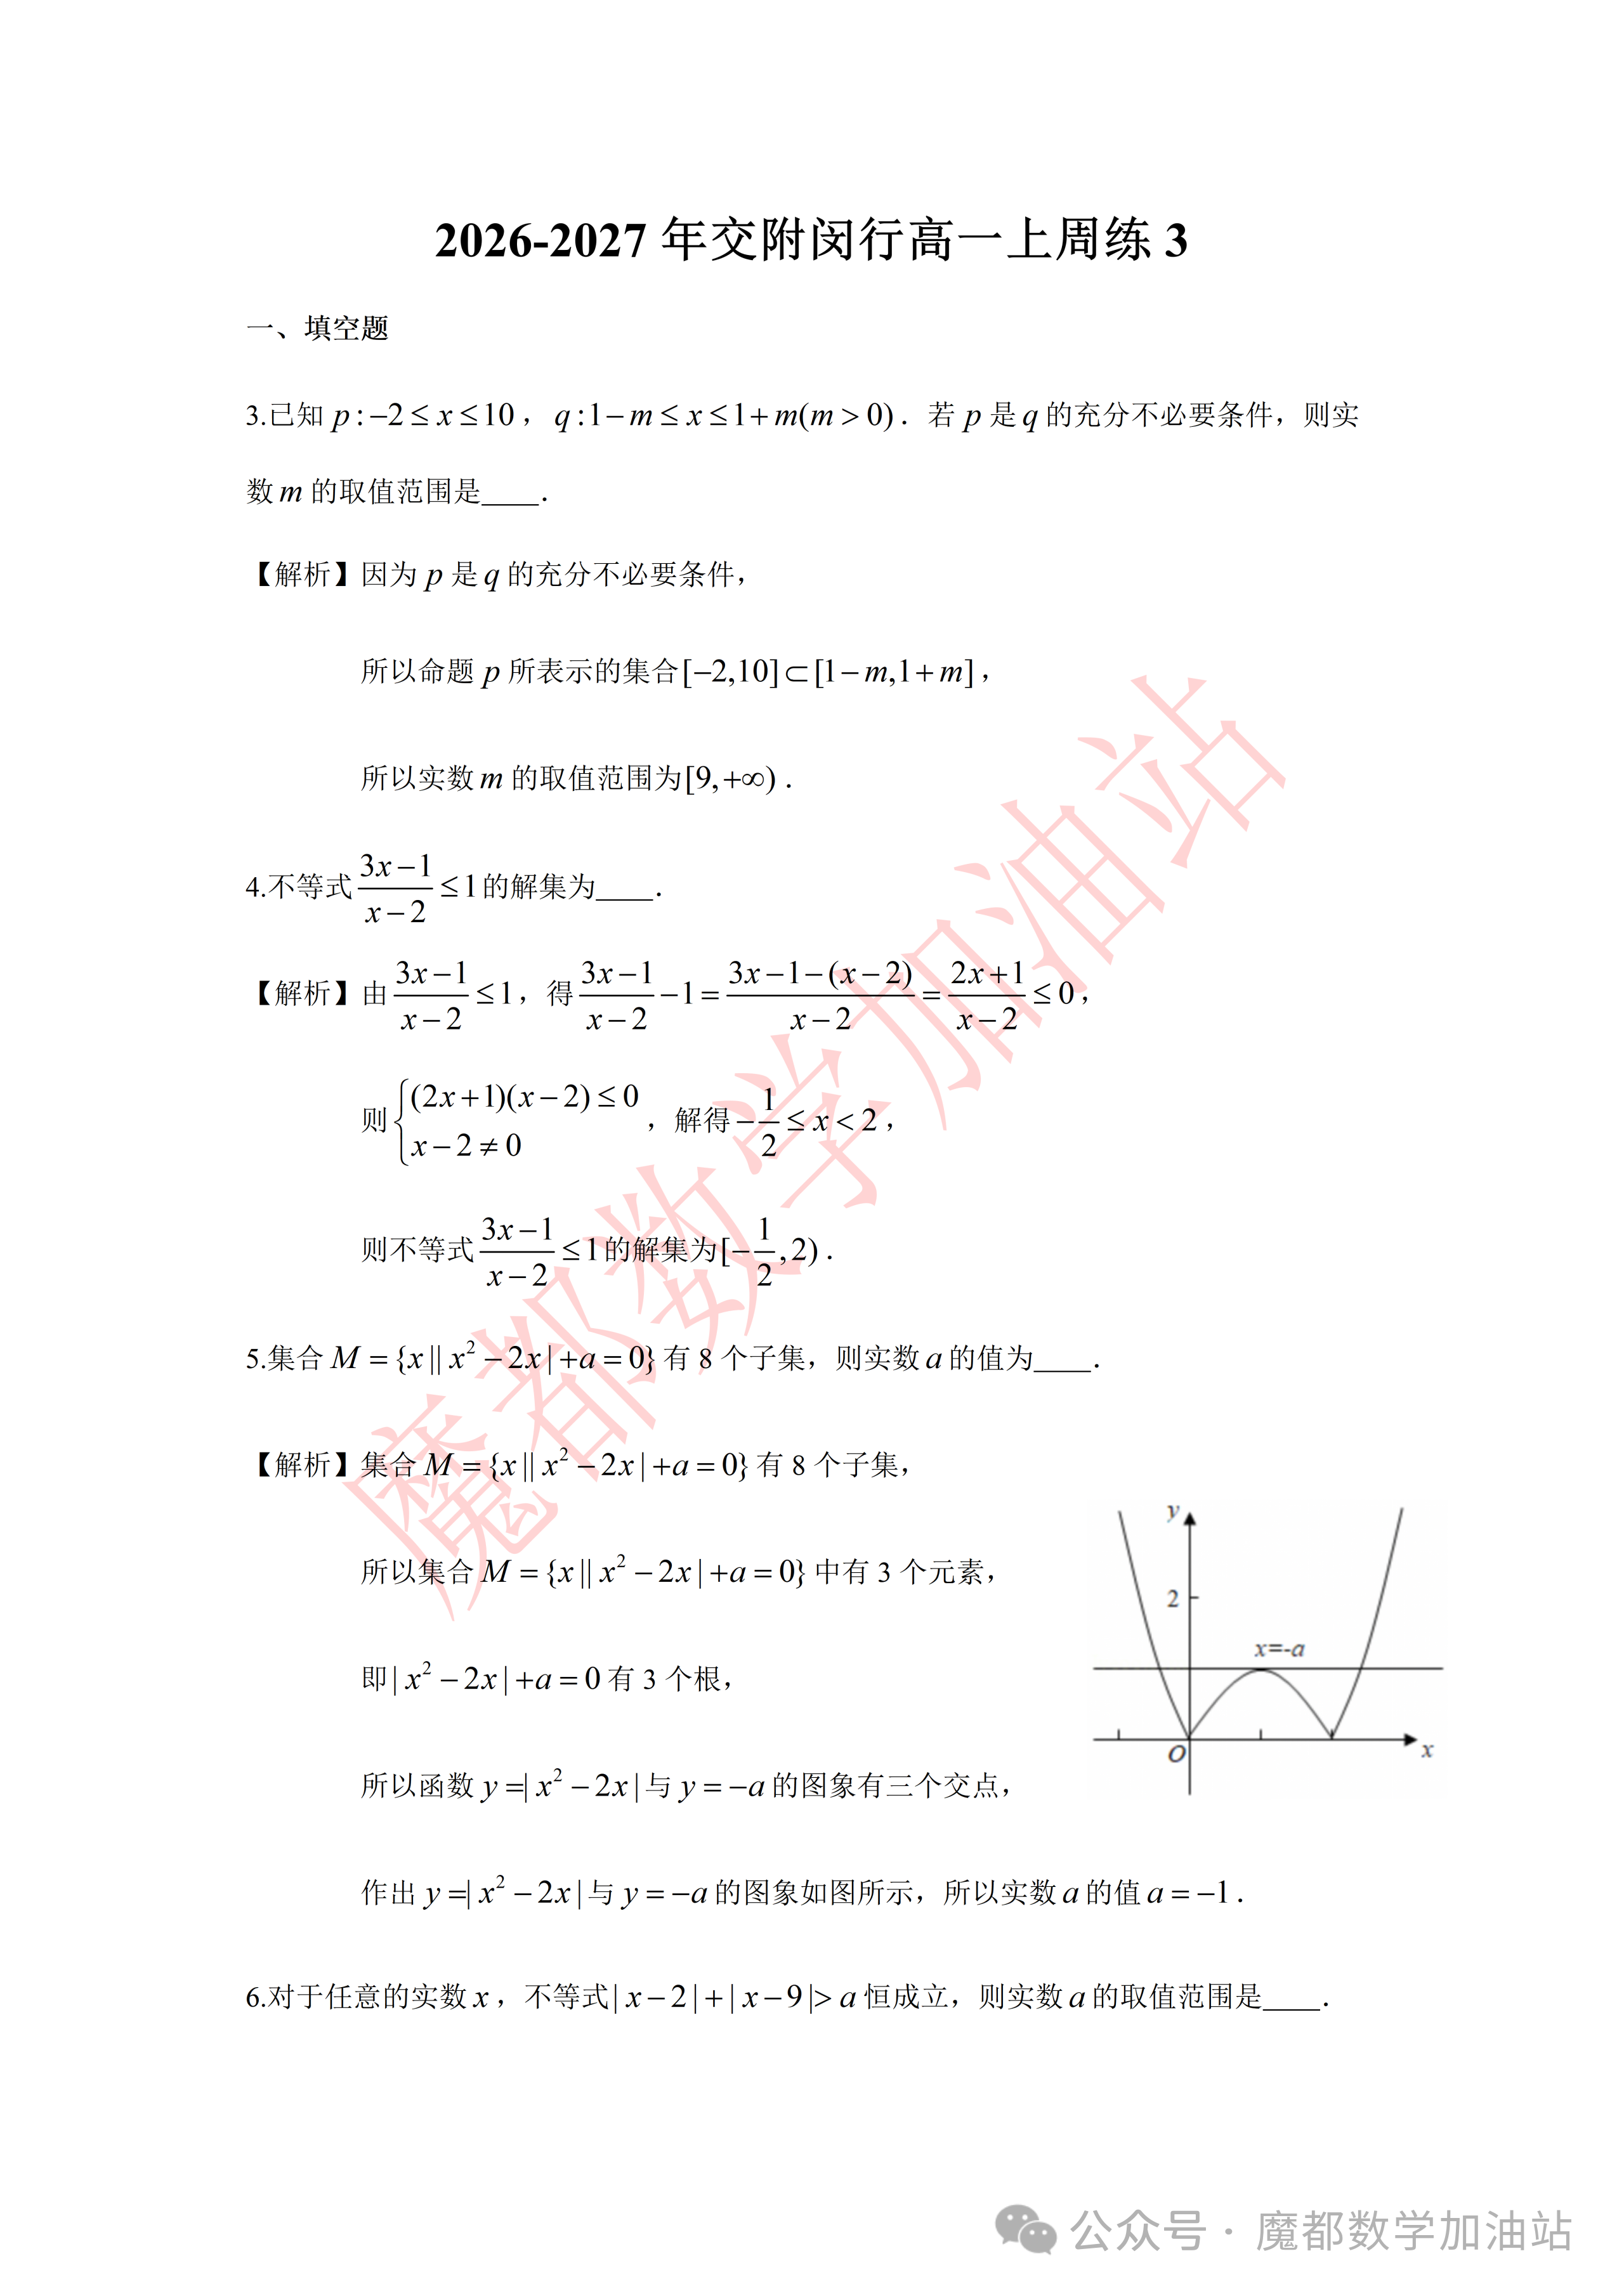
\includegraphics[width=0.14\textwidth,trim={1721bp 837bp 280bp 2297bp},clip]{../原图/高一43_交附闵行_周练3/01.png}
\end{center}

\solbegin
\step{集合 $M=\{x\mid |x^2-2x|+a=0\}$ 有 8 个子集，}
\step{所以集合 $M=\{x\mid |x^2-2x|+a=0\}$ 中有 3 个元素，}
\step{即 $|x^2-2x|+a=0$ 有 3 个根，}
\step{所以函数 $y=|x^2-2x|$ 与 $y=-a$ 的图象有三个交点，}
\step{作出 $y=|x^2-2x|$ 与 $y=-a$ 的图象如图所示，所以实数 $a$ 的值 $a=-1$.}
\solend

\fi

\item 对于任意的实数 $x$，不等式 $|x-2|+|x-9|>a$ 恒成立，则实数 $a$ 的取值范围是 \blankline[4.4em].

\ifanswer
\solbegin
\step{由绝对值的几何意义得 $|x-2|+|x-9|\geqslant7$，当且仅当 $2\leqslant x\leqslant9$ 时等号成立，}
\step{所以 $a<7$，}
\step{即 $a$ 的取值范围为 $(-\infty,7)$.}
\solend

\fi

\item 已知集合 $A=\{x\mid(a-1)x^2+3x-2=0\}$，$B=\{x\mid x^2-3x+2=0\}$，$A\subseteq B$，求实数 $a$ 的取值范围是 \blankline[4.4em].

\ifanswer
\solbegin
\step{由方程 $x^2-3x+2=0$，解得 $x=1$ 或 $x=2$，即 $B=\{1,2\}$，}
\step{因为 $A\subseteq B$，所以 $A=\varnothing$ 或 $A=\{1\}$ 或 $A=\{2\}$ 或 $A=\{1,2\}$，}
\step{当 $A=\varnothing$ 时，$a\neq1$，且 $\Delta=3^2-4(a-1)\times(-2)<0$，解得 $a<-\dfrac18$，}
\step{将 $x=1$ 代入方程 $(a-1)x^2+3x-2=0$，得 $a=0$，}
\step{此时 $A=\{x\mid-x^2+3x-2=0\}=\{1,2\}$，满足条件，}
\step{将 $x=2$ 代入方程 $(a-1)x^2+3x-2=0$，得到 $a=0$，上面已经验证满足条件，}
\step{综上所述，$a$ 的取值范围是 $\left(-\infty,-\dfrac18\right)\cup\{0\}$.}
\solend

\fi

\item 已知 $a$、$b$、$c$、$d$ 为常数，若不等式
$\dfrac{b}{x+a}+\dfrac{x+d}{x+c}<0$ 的解集为 $\left(-1,-\dfrac13\right)\cup\left(\dfrac12,1\right)$，
则不等式 $\dfrac{bx}{ax-1}+\dfrac{dx-1}{cx-1}<0$ 的解集为 \blankline[4.4em].

\ifanswer
\solbegin
\step{若 $x=0$，原不等式化为 $1<0$，不等式显然不成立，所以 $x\neq0$，}
\step{由 $\dfrac{bx}{ax-1}+\dfrac{dx-1}{cx-1}<0$，得 $\dfrac{b}{a-\dfrac1x}+\dfrac{d-\dfrac1x}{c-\dfrac1x}<0$，即 $\dfrac{b}{-\dfrac1x+a}+\dfrac{-\dfrac1x+d}{-\dfrac1x+c}<0$.}
\step{因为不等式 $\dfrac{b}{x+a}+\dfrac{x+d}{x+c}<0$ 的解集为 $\left(-1,-\dfrac13\right)\cup\left(\dfrac12,1\right)$，}
\step{所以 $-1<-\dfrac1x<-\dfrac13$ 或 $\dfrac12<-\dfrac1x<1$，解得 $1<x<3$ 或 $-2<x<-1$，}
\step{所以不等式 $\dfrac{bx}{ax-1}+\dfrac{dx-1}{cx-1}<0$ 的解集为 $(-2,-1)\cup(1,3)$.}
\solend

\fi

\item 正实数 $x$、$y$ 满足 $2x+3y-xy=0$，且存在这样的 $x$、$y$ 使不等式 $x+y<m+1$ 有解，则实数 $m$ 的取值范围是 \blankline[4.4em].

\ifanswer
\solbegin
\step{因为正实数 $x$、$y$ 满足 $2x+3y-xy=0$，则 $\dfrac2y+\dfrac3x=1$，$x>0$，$y>0$，}
\step{所以 $x+y=(x+y)\left(\dfrac3x+\dfrac2y\right)=3+\dfrac{2x}{y}+\dfrac{3y}{x}+2\geqslant2\sqrt{\dfrac{2x}{y}\times\dfrac{3y}{x}}+5=5+2\sqrt6$，}
\step{当且仅当 $\sqrt2x=\sqrt3y$ 时取等号，}
\step{存在这样的 $x$、$y$ 使不等式 $x+y<m+1$ 有解，则 $m+1>5+2\sqrt6$，}
\step{则 $m>4+2\sqrt6$，所以实数 $m$ 的取值范围是 $(4+2\sqrt6,+\infty)$.}
\solend

\fi

\item 若 $a$、$b$、$c\in\R$，$a^2+b^2+c^2=1$，则 $2ab+bc$ 的最大值为 \blankline[4.4em].

\ifanswer
\solbegin
\step{对于 $2ab+bc$，将 $b^2$ 拆分为 $\dfrac45b^2+\dfrac15b^2$，则 $a^2+\dfrac45b^2+c^2+\dfrac15b^2=1$，}
\step{$a^2+\dfrac45b^2\geqslant2\cdot a\cdot\dfrac2{\sqrt5}b=\dfrac4{\sqrt5}ab$，$c^2+\dfrac15b^2\geqslant2\cdot c\cdot\dfrac1{\sqrt5}b=\dfrac2{\sqrt5}bc$，}
\step{两式相加得 $1\geqslant\dfrac4{\sqrt5}ab+\dfrac2{\sqrt5}bc=\dfrac2{\sqrt5}(2ab+bc)$，故 $2ab+bc\leqslant\dfrac{\sqrt5}2$，}
\step{等号成立当且仅当 $a=\dfrac2{\sqrt5}b$，$c=\dfrac1{\sqrt5}b$，}
\step{代入 $a^2+b^2+c^2=1$，得 $\dfrac45b^2+b^2+\dfrac15b^2=2b^2=1$，即 $b=\dfrac{\sqrt2}2$，}
\step{此时 $a=\dfrac{\sqrt{10}}5$，$c=\dfrac{\sqrt{10}}{10}$，故 $2ab+bc$ 的最大值为 $\dfrac{\sqrt5}2$.}
\solend

\fi

\item 已知实数 $a$、$b$ 满足 $-3<a+2b<2$，$-1<2a-b<4$，则 $a+b$ 的取值范围为 \blankline[4.4em].

\ifanswer
\solbegin
\step{设 $a+b=m(a+2b)+n(2a-b)=(m+2n)a+(2m-n)b$，}
\step{所以 $\begin{cases}m+2n=1\\2m-n=1\end{cases}$，解得 $n=\dfrac15$，$m=\dfrac35$，所以 $a+b=\dfrac35(a+2b)+\dfrac15(2a-b)$，}
\step{因为 $-3<a+2b<2$，$-1<2a-b<4$，}
\step{所以 $-\dfrac95<\dfrac35(a+2b)<\dfrac65$，$-\dfrac15<\dfrac15(2a-b)<\dfrac45$，}
\step{相加得 $-2<\dfrac35(a+2b)+\dfrac15(2a-b)<2$，即 $-2<a+b<2$，}
\step{故 $a+b$ 的取值范围为 $(-2,2)$.}
\solend

\fi

% 注：原卷题干与解析均印作 \sqrt{2xyz}，但按其自身答案 8 与取等值（$y=\dfrac12$，
% $x=\dfrac{\sqrt3}4$，$z=\dfrac{\sqrt6}4$）代入只与 $\sqrt{2x^2y^2z^2}=\sqrt2\,xyz$ 相符，
% $\sqrt{2xyz}$ 与答案 8 不自洽，原卷如此，照录未改。
\item 已知正数 $x$、$y$、$z$ 满足 $2x^2+y^2+z^2=1$，则 $\dfrac{y+1}{\sqrt{2xyz}}$ 的最小值为 \blankline[4.4em].

\ifanswer
\solbegin
\step{由条件得 $2x^2+z^2=1-y^2=(1-y)(1+y)$，则 $1+y=\dfrac{2x^2+z^2}{1-y}$，}
\step{结合 $x$、$y$、$z>0$ 得原式 $=\dfrac{2x^2+z^2}{\sqrt{2xyz}(1-y)}\geqslant\dfrac{2\sqrt2xz}{\sqrt{2xyz}(1-y)}=\dfrac2{y(1-y)}$，}
\step{又 $y(1-y)\leqslant\left(\dfrac{y+1-y}2\right)^2=\dfrac14$，所以 $\dfrac2{y(1-y)}\geqslant\dfrac2{\frac14}=8$，}
\step{当且仅当 $\sqrt2x=z$，且 $y=1-y$，即 $y=\dfrac12$，$x=\dfrac{\sqrt3}4$，$z=\dfrac{\sqrt6}4$ 时取等号，}
\step{故 $\dfrac{y+1}{\sqrt{2xyz}}$ 最小值为 $8$.}
\solend

\fi

\end{enumerate}

\bigsec{二、选择题}

\begin{enumerate}
\setcounter{enumi}{12}

\item 已知关于 $x$ 的方程 $(1-k)x^2-2x-1=0$ 有实数根，则 $k$ 的取值范围是\mbox{（\quad）}

\keepwithprev
A. $k\leqslant2$ 且 $k\neq1$\qquad B. $k\leqslant2$\qquad
C. $k<2$ 且 $k\neq1$\qquad D. $k<2$

\ans{$A$}

\ifanswer
\solbegin
\step{由题意得 $\begin{cases}1-k\neq0\\\Delta=4+4(1-k)\geqslant0\end{cases}$，解不等式得 $\begin{cases}1\neq k\\2-k>0\end{cases}$，所以 $k\leqslant2$ 且 $k\neq1$，}
\step{故选 $A$.}
\solend

\fi

\item 不等式 $2|x+2|+|x-1|\geqslant5$ 成立的一个必要不充分条件是\mbox{（\quad）}

\keepwithprev
A. $x\leqslant-1$ 或 $x\geqslant0$\qquad B. $x\geqslant0$

C. $x\leqslant-\dfrac83$ 或 $x\geqslant0$\qquad D. $x\geqslant1$

\ans{$A$}

\ifanswer
\solbegin
\step{当 $x<-2$ 时，原不等式可化为 $-2x-4-x+1\geqslant5$，解得 $x\leqslant-\dfrac83$，}
\step{当 $-2\leqslant x<1$ 时，原不等式可化为 $2x+4-x+1\geqslant5$，解得 $0\leqslant x<1$，}
\step{当 $x\geqslant1$ 时，原不等式可化为 $2x+4+x-1\geqslant5$，解得 $x\geqslant\dfrac23$，得 $x\geqslant1$，}
\step{综上所述，不等式 $2|x+2|+|x-1|\geqslant5$ 成立的充要条件是 $x\leqslant-\dfrac83$ 或 $x\geqslant0$，}
\step{设 $A=\{x\mid x\leqslant-\dfrac83\text{ 或 }x\geqslant0\}$，}
\step{则不等式 $2|x+2|+|x-1|\geqslant5$ 成立的必要不充分条件，}
\step{其对应的集合 $B$ 满足 $A\subsetneq B$，对照各个选项，$A$ 项符合题意. 故选 $A$.}
\solend

\fi

\item 已知实数 $a>0$，$b>0$，$\dfrac1{a+1}+\dfrac1{b+1}=1$，则 $2a+3b$ 的最小值为\mbox{（\quad）}

\keepwithprev
A. $2\sqrt6$\qquad B. $3+2\sqrt6$\qquad
C. $5+2\sqrt6$\qquad D. $3+2\sqrt2$

\ans{$A$}

\ifanswer
\solbegin
\step{因为 $a>0$，$b>0$，$\dfrac1{a+1}+\dfrac1{b+1}=1$，}
\step{所以 $2a+3b=2(a+1)+3(b+1)-5=[2(a+1)+3(b+1)]\cdot\left(\dfrac1{a+1}+\dfrac1{b+1}\right)-5$}
\step{$=\left[2+3+\dfrac{3(b+1)}{a+1}+\dfrac{2(a+1)}{b+1}\right]-5\geqslant5+2\sqrt{\dfrac{3(b+1)}{a+1}\times\dfrac{2(a+1)}{b+1}}-5=2\sqrt6$，}
\step{当且仅当 $\dfrac{3(b+1)}{a+1}=\dfrac{2(a+1)}{b+1}$，即 $a=\dfrac{\sqrt6}2$，$b=\dfrac{\sqrt6}3$ 时取等号. 故选 $A$.}
\solend

\fi

\item 已知集合 $U=\{n\mid1\leqslant n\leqslant2027,\ n\in\N\}$，集合 $M\subseteq U$，若对于 $M$ 中任意两个不同的元素 $x$ 和 $y$，都有 $|x-y|>2$，则 $M$ 中元素个数的最大值是\mbox{（\quad）}

\keepwithprev
A. $676$\qquad B. $675$\qquad C. $672$\qquad D. $671$

\ans{$A$}

\ifanswer
\solbegin
\step{对于 $M$ 中的任意两个不同的元素 $x$、$y$，都有 $|x-y|>2$，}
\step{不妨设 $x>y$，都有 $x-y\geqslant3$，}
\step{要想 $M$ 所含元素个数最大，则要 $x-y$ 尽可能小，故需使得 $x-y$ 的最小值为 3，}
\step{将 $1\sim2027$ 这 2027 个元素按如下分组：}
\step{$\{1,2,3\}$，$\{4,5,6\}$，$\cdots$，$\{2023,2024,2025\}$，$\{2026,2027\}$，}
\step{故应在前 675 组中按周期 3 每组取一个元素，且第一组中不能取 3，}
\step{第一组中取 1 时，得 $M=\{1,4,7,\cdots,2023,2026\}$，}
\step{或 $M=\{1,4,7,\cdots,2023,2027\}$ 这样的集合，}
\step{第一组取 2 时，得 $M=\{2,5,8,\cdots,2024,2027\}$，}
\step{其中任意两元素差值 $x-y$（$x>y$）都大于 2，满足题意，}
\step{故 $M$ 所含元素个数的最大值为 $\dfrac{2025}{3}+1=676$. 故选 $A$.}
\solend

\fi

\end{enumerate}

\bigsec{三、解答题}

\begin{enumerate}
\setcounter{enumi}{16}

\item 已知 $a\in\R$，集合 $A=\left\{x\middle|\dfrac{2-x}{x+1}\leqslant0\right\}$，$B=\{x\mid x^2+(3-a)x-3a<0\}$.

\begin{enumerate}[label=(\arabic*)]
\item 当 $a=\dfrac13$ 时，求 $A$ 和 $B$；
\item 已知 $A\cup B=A$，求实数 $a$ 的取值范围.
\end{enumerate}

\ifanswer
\solbegin
\stepm{(1)}{由 $\dfrac{2-x}{x+1}\leqslant0$，得 $\begin{cases}(2-x)(x+1)\leqslant0\\x\neq-1\end{cases}$，解得 $x<-1$ 或 $x\geqslant2$，}
\step{则 $A=\{x\mid x<-1\text{ 或 }x\geqslant2\}$；}
\step{$B=\{x\mid x^2+(3-a)x-3a<0\}=\{x\mid(x+3)(x-a)<0\}$，}
% 注：原卷此行印作 $(x+2)\left(x-\dfrac13\right)$，按前一行 $B=\{x\mid(x+3)(x-a)<0\}$ 应为
% $(x+3)\left(x-\dfrac13\right)$，原卷如此，照录未改。
\step{当 $a=\dfrac13$ 时，$B=\left\{x\middle|(x+2)\left(x-\dfrac13\right)<0\right\}$，}
\step{解得 $B=\left\{x\middle|-3<x<\dfrac13\right\}$.}
\stepm{(2)}{由 $A\cup B=A$，得 $B\subseteq A$，}
\step{①当 $B=\varnothing$ 时，得 $a=-3$，符合题意；}
\step{②当 $B\neq\varnothing$ 时，若 $a>-3$，则 $B=\{x\mid-3<x<a\}$，}
\step{由 $B\subseteq A$，得 $a\leqslant-1$，此时 $-3<a\leqslant-1$；}
\step{若 $a<-3$，则 $B=\{x\mid a<x<-3\}$，此时 $B\subseteq A$ 恒成立，}
\step{故 $a<-3$ 符合题意；}
\step{综上所述，实数 $a$ 的取值范围为 $a\leqslant-1$.}
\solend

\fi

\ansspace[6]

\item 甲乙两地的高速公路全长 166 千米，汽车从甲地进入该高速公路后匀速行驶到乙地，车速 $v\in[70,120]$（千米/时）. 已知汽车每小时的运输成本（以元为单位）由可变部分和固定部分组成：可变部分为 $0.02v^2$，固定部分为 220 元.

\begin{enumerate}[label=(\arabic*)]
\item 若每小时的运输成本不高于 420 元，汽车的速度应该控制在什么范围？
\item 汽车应以多大速度行驶才能使全程运输成本最小？最小运输成本约为多少元？（结果保留整数）
\end{enumerate}

\ifanswer
\solbegin
\stepm{(1)}{已知汽车每小时的运输成本（以元为单位）由可变部分和固定部分组成：}
\step{可变部分为 $0.02v^2$，固定部分为 220 元，}
\step{则汽车每小时的运输成本为 $0.02v^2+220$（元），}
\step{若每小时的运输成本不高于 420 元，}
\step{则 $0.02v^2+220\leqslant420$，解得 $v^2\leqslant10000$，}
\step{得 $70\leqslant v\leqslant100$，即 $v\in[70,100]$（千米/时），}
\step{则此时汽车的速度 $v$ 应该控制在 $[70,100]$（千米/时）；}
\stepm{(2)}{因为汽车从甲地进入该高速公路后匀速行驶到乙地，}
\step{车速 $v\in[70,120]$（千米/时），所以汽车的行驶时间为 $\dfrac{166}{v}$（小时），}
\step{所以全程运输成本 $y=\dfrac{166}{v}(0.02v^2+220)=3.32v+\dfrac{36520}{v}$，}
% 注：原卷此行印作 $v\in[70,100]$，与题干的 $v\in[70,120]$ 不自洽（若 $v\in[70,100]$，
% 最小值应在 $v=100$ 处取得，与下文 $v=10\sqrt{110}\approx105$ 矛盾），原卷如此，照录未改。
\step{$v\in[70,100]$，}
\step{由基本不等式得 $y=3.32v+\dfrac{36520}{v}\geqslant2\sqrt{3.32v\times\dfrac{36520}{v}}\approx696$，}
\step{当且仅当 $3.32v=\dfrac{36520}{v}$，即 $v=10\sqrt{110}\approx105$ 时取等号，}
\step{汽车应以 105（千米/时）行驶才能使全程运输成本最小，}
\step{最小运输成本约为 696 元.}
\solend

\fi

\ansspace[8]

\item
\begin{enumerate}[label=(\arabic*)]
\item 已知 $a$、$b$、$c$ 为实数，求证：$|a-b|\leqslant|a-c|+|b-c|$，并说明等号成立的条件；
\item 设 $x\in\R$，求方程 $|3x-8|=|5-x|+|2x-3|$ 的解集.
\end{enumerate}

\ifanswer
% 注：原卷第 19 题未印【解析】，仅印一行【答案】"（1）(a-c)(b-c)≤0；
% （2）(-∞,3/2]∪[5,+∞)"。(1) 的两行推导为本稿所补，(2) 照录原卷答案。
% 又题干作"方程"，而所给答案 (-∞,3/2]∪[5,+∞) 实为不等式 |3x-8|≤|5-x|+|2x-3| 的解集，
% 与"方程"不合，原卷如此，照录未改。
\solbegin
\stepm{(1)}{由三角不等式 $|a-b|=|(a-c)-(b-c)|\leqslant|a-c|+|b-c|$，}
\step{当且仅当 $(a-c)(b-c)\leqslant0$ 时等号成立.}
\stepm{(2)}{$\left(-\infty,\dfrac32\right]\cup[5,+\infty)$.}
\solend

\fi

\ansspace[6]

\item 已知正实数 $a$、$b$ 满足 $a+b=1$，求 $\dfrac1a+\dfrac1b$ 的最小值. 其中一种解法是：

\[
\begin{aligned}
\dfrac1a+\dfrac1b
&=\left(\dfrac1a+\dfrac1b\right)(a+b)\\
&=1+\dfrac ba+\dfrac ab+1\\
&\geqslant2+2\sqrt{\dfrac ba\times\dfrac ab}=2+2=4.
\end{aligned}
\]
当且仅当 $\dfrac ba=\dfrac ab$ 且 $a+b=1$ 时即 $a=b=\dfrac12$ 时取等号.
学习上述解法并解决下列问题：

\begin{enumerate}[label=(\arabic*)]
\item 若正实数 $x$、$y$ 满足 $x+y=xy$，求 $2x+y$ 的最小值；
\item 若实数 $a$、$b$、$x$、$y$ 满足 $\dfrac{x^2}{a^2}+\dfrac{y^2}{b^2}=1$，求证：$a^2+b^2\geqslant(x+y)^2$；
\item 求代数式 $M=\sqrt{m-1}+\sqrt{3-m}$ 的最大值，并求出使得 $M$ 最大的 $m$ 的值.
\end{enumerate}

\ifanswer
\solbegin
\stepm{(1)}{因为正实数 $x$、$y$ 满足 $x+y=xy$，$\dfrac{x+y}{xy}=1\Rightarrow\dfrac1y+\dfrac1x=1$，}
\step{所以 $(2x+y)\times1=(2x+y)\left(\dfrac1y+\dfrac1x\right)=3+\dfrac{2x}{y}+\dfrac yx\geqslant3+2\sqrt{\dfrac{2x}{y}\cdot\dfrac yx}=3+2\sqrt2$，}
\step{当且仅当 $\dfrac{2x}{y}=\dfrac yx$ 且 $\dfrac1y+\dfrac1x=1$ 时取等号，}
\step{解得 $x=\dfrac{2+\sqrt2}2$，$y=\sqrt2x=\sqrt2\times\dfrac{2+\sqrt2}2=1+\sqrt2$，}
\step{所以 $2x+y$ 的最小值为 $3+2\sqrt2$；}
\stepm{(2)}{因为 $\dfrac{x^2}{a^2}+\dfrac{y^2}{b^2}=1$，}
\step{所以 $a^2+b^2=(a^2+b^2)\left(\dfrac{x^2}{a^2}+\dfrac{y^2}{b^2}\right)=x^2+y^2+\dfrac{b^2x^2}{a^2}+\dfrac{a^2y^2}{b^2}$，}
\step{因为 $\dfrac{b^2x^2}{a^2}+\dfrac{a^2y^2}{b^2}\geqslant2\sqrt{\dfrac{b^2x^2}{a^2}\times\dfrac{a^2y^2}{b^2}}=2\sqrt{x^2y^2}=2|xy|$，}
\step{当且仅当 $\dfrac{b^2x^2}{a^2}=\dfrac{a^2y^2}{b^2}$ 时取等号，}
\step{所以 $x^2+y^2+\dfrac{b^2x^2}{a^2}+\dfrac{a^2y^2}{b^2}\geqslant x^2+y^2+2|xy|\geqslant x^2+y^2+2xy=(x+y)^2$，}
\step{所以 $a^2+b^2\geqslant(x+y)^2$；}
\stepm{(3)}{因为 $M=\sqrt{m-1}+\sqrt{3-m}$，所以 $\begin{cases}m-1\geqslant0\\3-m\geqslant0\end{cases}$，解得 $1\leqslant m\leqslant3$，}
\step{所以 $M^2=(\sqrt{m-1}+\sqrt{3-m})^2=2+2\sqrt{(3-m)(m-1)}$，}
\step{由基本不等式得 $(3-m)(m-1)\leqslant\left(\dfrac{(3-m)+(m-1)}2\right)^2=1$，}
\step{当且仅当 $3-m=m-1$ 时取等号，解得 $m=2$，}
\step{所以 $M^2=2+2\sqrt{(3-m)(m-1)}\leqslant2+2\sqrt1=4$，}
\step{因为 $M>0$，所以 $M\leqslant2$，所以 $M$ 最大值为 2，此时 $m$ 的值为 2.}
\solend

\fi

\ansspace[8]

\item 若有限个正整数组成的集合 $A$ 中至少有两个元素，且对于任意的 $x,y\in A$（$x>y$），都有 $\dfrac{y^2}{x-y}\in A$，则称 $A$ 为“L-集合”.

\begin{enumerate}[label=(\arabic*)]
\item 判断 $\{1,2,4\}$ 是否为“L-集合”，说明理由；
\item 若双元素集 $M$ 为“L-集合”，且 $4\in M$，求所有满足条件的集合 $M$；
\item 求所有满足条件的“L-集合”.
\end{enumerate}

\ifanswer
\solbegin
\stepm{(1)}{若至少由两个元素构成的有限集合 $A\subseteq\N^*$，}
% 注：原卷下一行"都有"后未印分数 \dfrac{y^2}{x-y}，径作"都有 A"，原卷如此，照录未改。
\step{且对于任意的 $x$、$y\in A$（$x>y$），都有 $A$，则称 $A$ 为“L-集合”，}
\step{$\{1,2,4\}$ 不为“L-集合”，理由如下：}
\step{因为 $\dfrac{1^2}{4-1}=\dfrac13\notin\{1,2,4\}$，所以 $\{1,2,4\}$ 不是“L-集合”.}
\stepm{(2)}{设 $M=\{4,m\}$（$m\in\N^*$，$m\neq4$），}
\step{若 $m<4$，则 $\dfrac{m^2}{4-m}=m$ 或 $\dfrac{m^2}{4-m}=4$，}
\step{由 $\dfrac{m^2}{4-m}=m$，解得 $m=2$，$m=0$（舍去），此时 $M=\{2,4\}$；}
\step{由 $\dfrac{m^2}{4-m}=4$ 化为 $m^2+4m-16=0$，而 $\Delta=4^2+4\times16=80$，}
\step{故方程无正整数解.}
\step{若 $m>4$，则 $\dfrac{4^2}{m-4}=4$ 或 $\dfrac{4^2}{m-4}=m$，}
\step{由 $\dfrac{4^2}{m-4}=4$，解得 $m=8$，此时 $M=\{4,8\}$；}
\step{由 $\dfrac{4^2}{m-4}=m$ 化为 $m^2-4m-16=0$，而 $\Delta=4^2+4\times16=80$，}
\step{故方程无正整数解.}
\step{综上，双元素集 $M$ 为“L-集合”，且 $4\in M$，}
\step{则所有满足条件的集合 $M$ 为 $\{4,8\}$，$\{2,4\}$.}
\stepm{(3)}{若“L-集合”为双元素集，}
\step{不妨设 $M=\{k,m\}$（$k,m\in\N^*$，$m>k$），则 $\dfrac{k^2}{m-k}=k$ 或 $\dfrac{k^2}{m-k}=m$，}
\step{由 $\dfrac{k^2}{m-k}=k$，则 $2k^2=mk$，而 $m>k$，故 $m=2k$，此时 $M=\{k,2k\}$；}
\step{由 $\dfrac{k^2}{m-k}=m$，则 $m^2-mk-k^2=0$，而 $\Delta=5k^2$，显然不存在正整数解；}
\step{所以，“L-集合”为 $\{k,2k\}$，其中 $k\in\N^*$.}
\step{若“L-集合”含有两个以上的元素，}
\step{设最小的元素为 $b$，最大的元素为 $a$，第二大的元素为 $n$，}
\step{则 $\dfrac{b^2}{a-b}$，$\dfrac{n^2}{a-n}$ 是“L-集合”中的元素，}
% 注：原卷下一行未印"由于'L-集合'中的元素均为正整数"一语，径作"若 \dfrac{b^2}{a-b}\geqslant b"，
% 原卷如此，照录未改。
\step{若 $\dfrac{b^2}{a-b}\geqslant b$，解得 $a\leqslant2b$，}
\step{若 $\dfrac{n^2}{a-n}\leqslant n$，则 $a\geqslant2n>2b$，矛盾，}
\step{若 $\dfrac{n^2}{a-n}=a$，该方程的解为 $n=\dfrac{\sqrt5-1}2a$，则 $n$、$a$ 不可能同时为整数，}
\step{无解.}
\step{所以所有满足条件的“L-集合”为 $\{k,2k\}$，其中 $k\in\N^*$.}
\solend

\fi

\ansspace*[10]

\end{enumerate}

\end{document}
"
% 紧凑版：xelatex "\def\iscompact{1}% 高一43_交附闵行_周练3.tex
%   —— 高一上数学“2026-2027 年交附闵行高一上周练3”（试卷版/答案版）
% 试卷版：xelatex 高一43_交附闵行_周练3.tex
% 答案版：xelatex "\def\isanswer{1}% 高一43_交附闵行_周练3.tex
%   —— 高一上数学“2026-2027 年交附闵行高一上周练3”（试卷版/答案版）
% 试卷版：xelatex 高一43_交附闵行_周练3.tex
% 答案版：xelatex "\def\isanswer{1}\input{高一43_交附闵行_周练3.tex}"
% 紧凑版：xelatex "\def\iscompact{1}\input{高一43_交附闵行_周练3.tex}"
%
% 原始材料是微信公众号图文（公众号“魔都数学加油站”，作者破晓，2026-10-01 21:37，
% 原文标题“27学年高一43——2026-2027年上海市交附闵行高一上周练3”，
% https://mp.weixin.qq.com/s/-rgkOD9jJVpug6s0uSbwmQ）。正文为 12 张 PNG 页；
% 第 01、05、09、12 页 2560×3620，其余第 02—04、06—08、10—11 页 4762×6735。
% 原文本身是讲评版，题目下方印有解析/答案；题目与讲解照原卷转录，保留原卷错误。
%
% 卷首标题：原卷印作“2026-2027 年交附闵行高一上周练3”，公众号标题中的“上海市”
% 三字不在卷面标题中，本稿依卷面录入；年份区间按全稿惯例排 en dash。
%
% 与原卷的排版差异：
%   ① 原文从第 3 题开始（第 1、2 题未在这篇推文中发布），本稿保留原题号 3—21；
%   ② 原卷本就印有“一、填空题”“二、选择题”“三、解答题”，本稿照原卷分节，
%      改排为全稿统一的大节标题；
%   ③ 原卷未印副标题，本稿按“知识模块”口径补出“集合与常用逻辑用语、不等式”；
%   ④ 原卷填空横线依全稿惯例排为 \blankline[4.4em]；选择题答案只在答案版以 \ans{} 显示，
%      解答区以 \ifanswer 分离；解答题按原卷留出标准作答空间；
%   ⑤ 第 5 题图取自原卷第 1 页截图并裁入本稿，不另建图档；公众号水印不录入。
%      原卷图页分页不保留，正文依本稿版心重新分页。
%
% 原卷存疑/错误（均照录，未改）：
%   ① 第 9 题原卷题干即作"正实数 x、y"，与解析 x>0、y>0 相容，并无矛盾（初稿曾误记
%      题干只称"实数"并据此指原卷不自洽，2026-10-05 回原图核对订正）。
%   ② 第 11 题解析"相加得"一行原卷印作 -2<3/5(a+2b)+1/5(2a-b)<2，第一项系数 3/5
%      原卷不缺（初稿漏抄致该行按字面不成立，2026-10-05 已按原卷补回）。
%   ③ 第 13 题答案印 A，解析以“1-k≠0”排除 k=1；但 k=1 时原方程为 -2x-1=0，
%      仍有实数根，按题意应选 B。本稿保留原卷答案 A 及其解析，不代为订正。
%
\documentclass[a4paper,11pt]{article}
\usepackage{common}
\usepackage{graphicx}

\begin{document}

\examtitlest[3]{2026--2027 年交附闵行高一上周练 3}{集合与常用逻辑用语、不等式}

\bigsec{一、填空题}

\begin{enumerate}
\setcounter{enumi}{2}

\item 已知 $p\colon -2\leqslant x\leqslant10$，$q\colon 1-m\leqslant x\leqslant1+m$（$m>0$）. 若 $p$ 是 $q$ 的充分不必要条件，则实数 $m$ 的取值范围是 \blankline[4.4em].

\ifanswer
\solbegin
\step{因为 $p$ 是 $q$ 的充分不必要条件，}
\step{所以命题 $p$ 所表示的集合 $[-2,10]\subset[1-m,1+m]$，}
\step{所以实数 $m$ 的取值范围为 $[9,+\infty)$.}
\solend

\fi

\item 不等式 $\dfrac{3x-1}{x-2}\leqslant1$ 的解集为 \blankline[4.4em].

\ifanswer
\solbegin
\step{由 $\dfrac{3x-1}{x-2}-1=\dfrac{3x-1-(x-2)}{x-2}=\dfrac{2x+1}{x-2}\leqslant0$，}
\step{则 $\begin{cases}(2x+1)(x-2)\leqslant0\\x-2\neq0\end{cases}$，解得 $-\dfrac12\leqslant x<2$，}
\step{则不等式 $\dfrac{3x-1}{x-2}\leqslant1$ 的解集为 $\left[-\dfrac12,2\right)$.}
\solend

\fi

\item 集合 $M=\{x\mid |x^2-2x|+a=0\}$ 有 8 个子集，则实数 $a$ 的值为 \blankline[4.4em].

\ifanswer
\begin{center}
% 图取自原卷第 1 页；用原图裁切，未重绘。
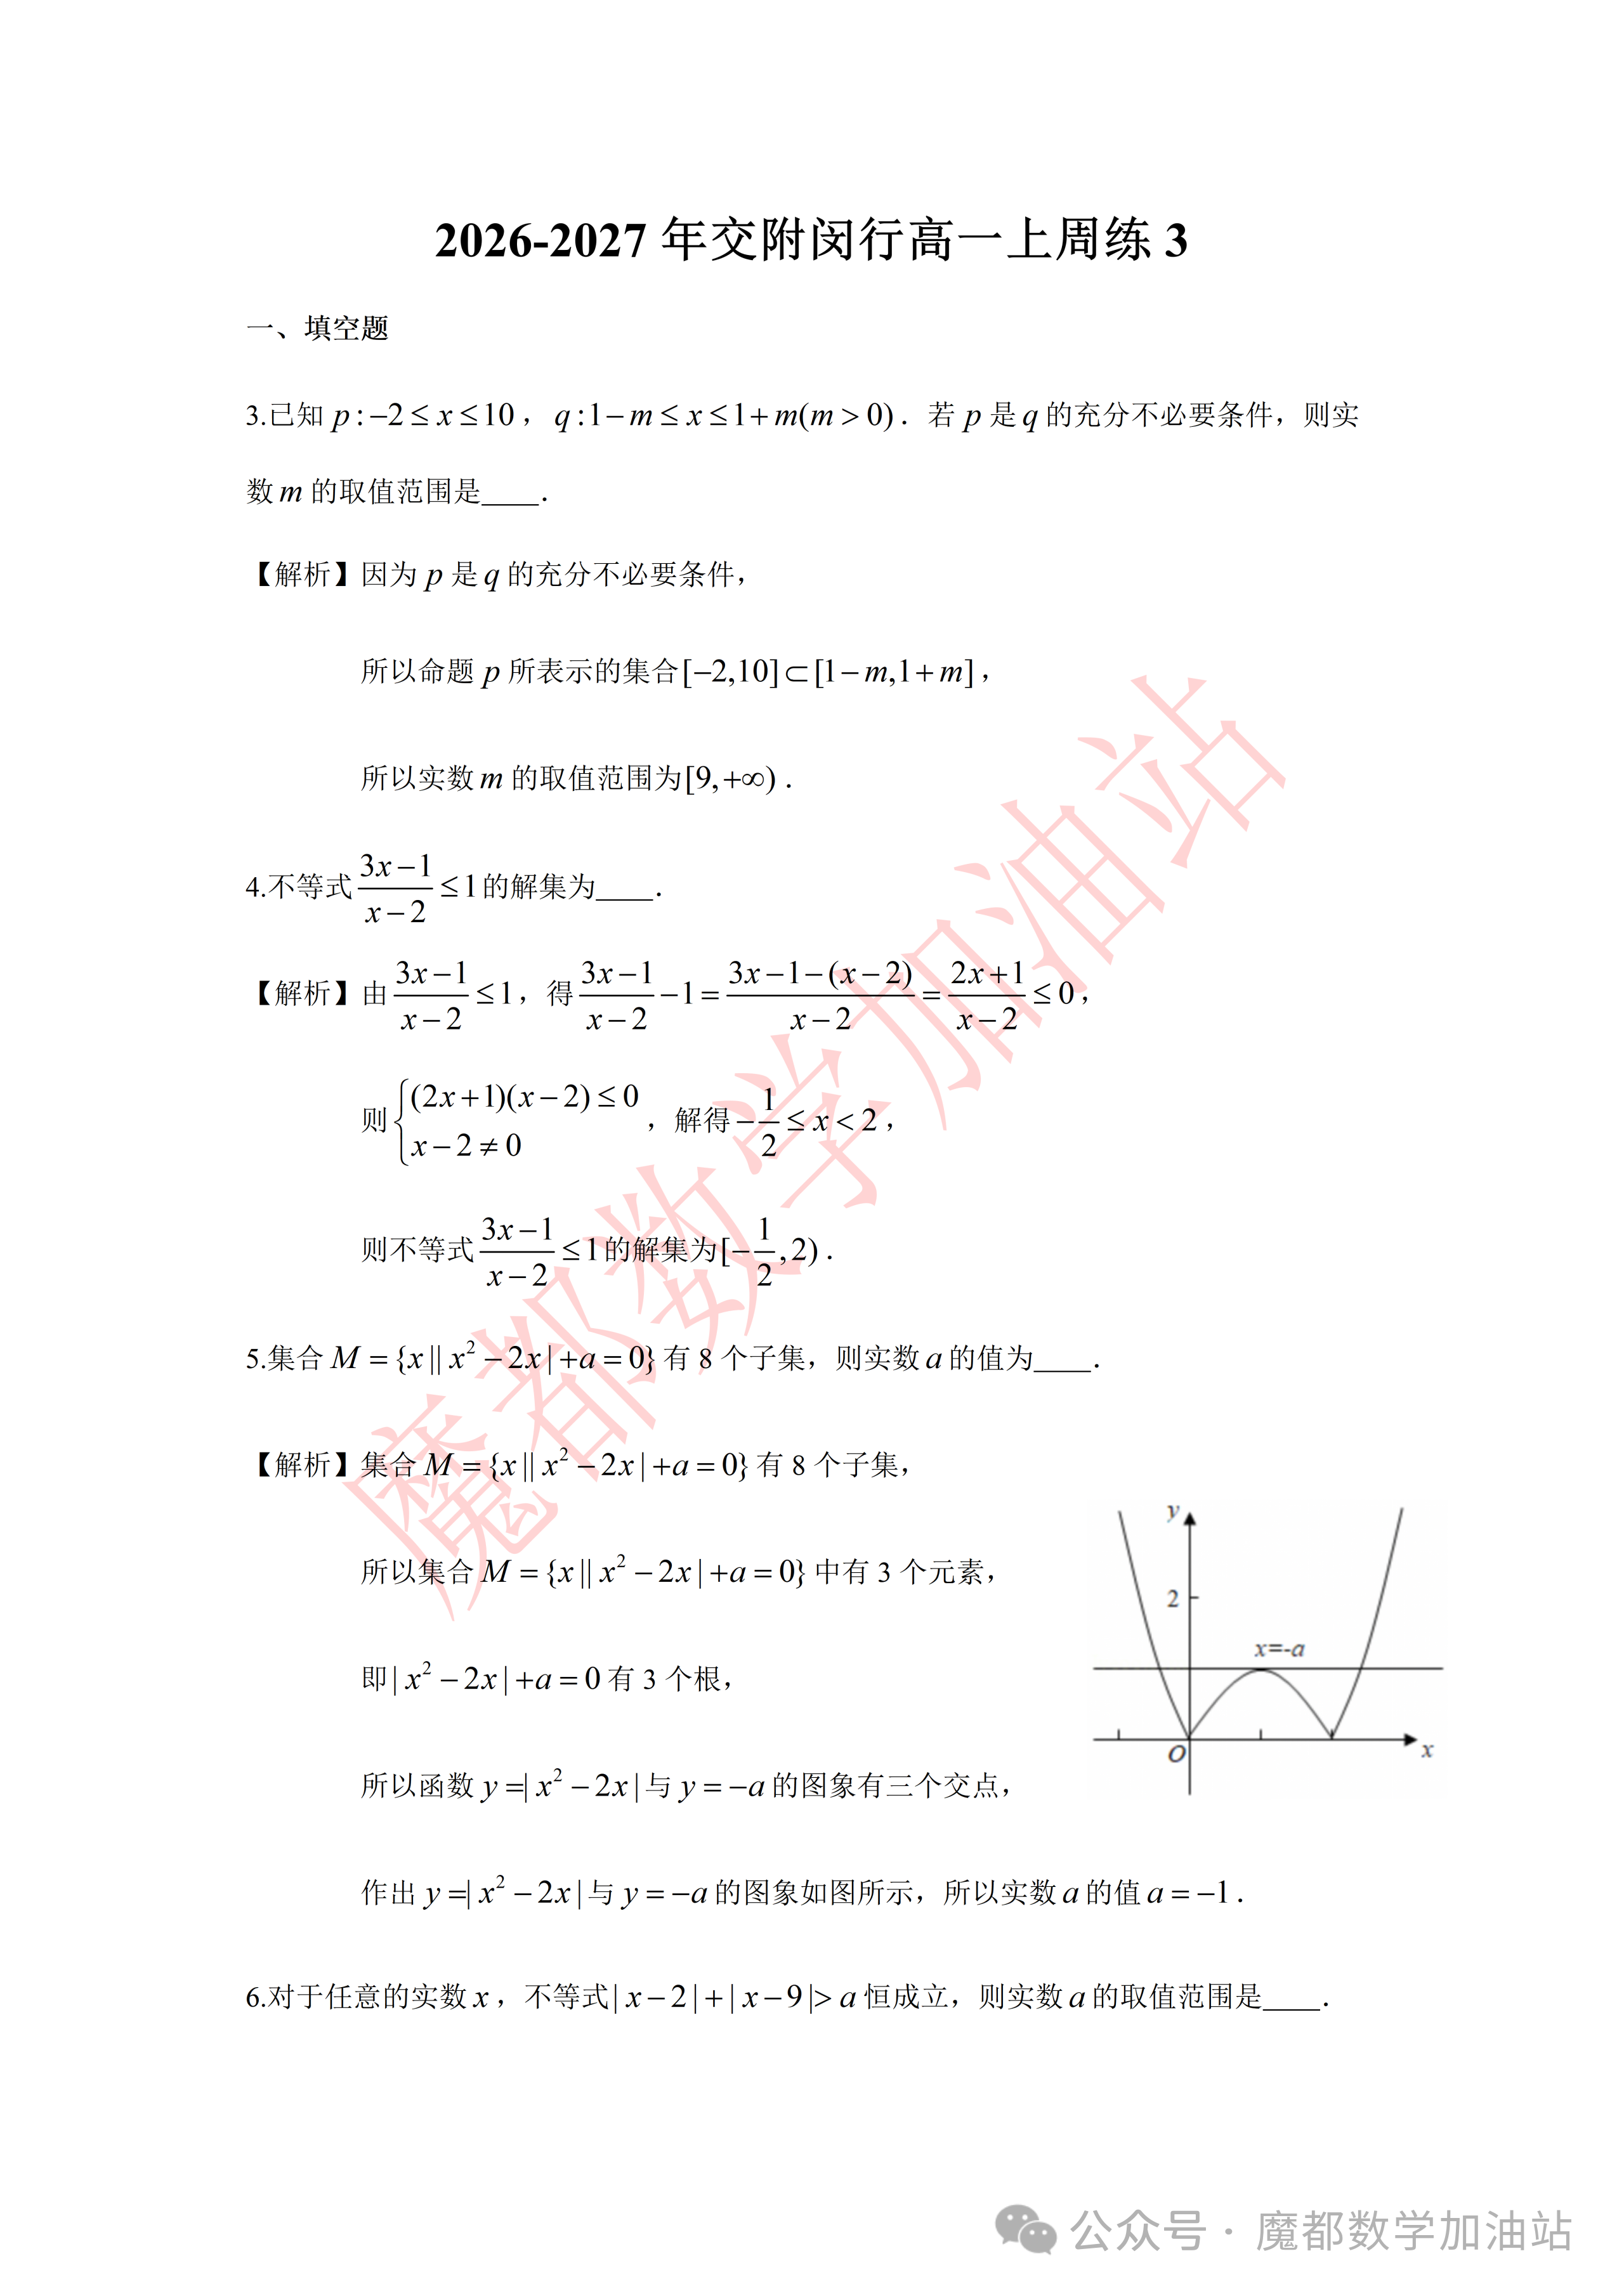
\includegraphics[width=0.14\textwidth,trim={1721bp 837bp 280bp 2297bp},clip]{../原图/高一43_交附闵行_周练3/01.png}
\end{center}

\solbegin
\step{集合 $M=\{x\mid |x^2-2x|+a=0\}$ 有 8 个子集，}
\step{所以集合 $M=\{x\mid |x^2-2x|+a=0\}$ 中有 3 个元素，}
\step{即 $|x^2-2x|+a=0$ 有 3 个根，}
\step{所以函数 $y=|x^2-2x|$ 与 $y=-a$ 的图象有三个交点，}
\step{作出 $y=|x^2-2x|$ 与 $y=-a$ 的图象如图所示，所以实数 $a$ 的值 $a=-1$.}
\solend

\fi

\item 对于任意的实数 $x$，不等式 $|x-2|+|x-9|>a$ 恒成立，则实数 $a$ 的取值范围是 \blankline[4.4em].

\ifanswer
\solbegin
\step{由绝对值的几何意义得 $|x-2|+|x-9|\geqslant7$，当且仅当 $2\leqslant x\leqslant9$ 时等号成立，}
\step{所以 $a<7$，}
\step{即 $a$ 的取值范围为 $(-\infty,7)$.}
\solend

\fi

\item 已知集合 $A=\{x\mid(a-1)x^2+3x-2=0\}$，$B=\{x\mid x^2-3x+2=0\}$，$A\subseteq B$，求实数 $a$ 的取值范围是 \blankline[4.4em].

\ifanswer
\solbegin
\step{由方程 $x^2-3x+2=0$，解得 $x=1$ 或 $x=2$，即 $B=\{1,2\}$，}
\step{因为 $A\subseteq B$，所以 $A=\varnothing$ 或 $A=\{1\}$ 或 $A=\{2\}$ 或 $A=\{1,2\}$，}
\step{当 $A=\varnothing$ 时，$a\neq1$，且 $\Delta=3^2-4(a-1)\times(-2)<0$，解得 $a<-\dfrac18$，}
\step{将 $x=1$ 代入方程 $(a-1)x^2+3x-2=0$，得 $a=0$，}
\step{此时 $A=\{x\mid-x^2+3x-2=0\}=\{1,2\}$，满足条件，}
\step{将 $x=2$ 代入方程 $(a-1)x^2+3x-2=0$，得到 $a=0$，上面已经验证满足条件，}
\step{综上所述，$a$ 的取值范围是 $\left(-\infty,-\dfrac18\right)\cup\{0\}$.}
\solend

\fi

\item 已知 $a$、$b$、$c$、$d$ 为常数，若不等式
$\dfrac{b}{x+a}+\dfrac{x+d}{x+c}<0$ 的解集为 $\left(-1,-\dfrac13\right)\cup\left(\dfrac12,1\right)$，
则不等式 $\dfrac{bx}{ax-1}+\dfrac{dx-1}{cx-1}<0$ 的解集为 \blankline[4.4em].

\ifanswer
\solbegin
\step{若 $x=0$，原不等式化为 $1<0$，不等式显然不成立，所以 $x\neq0$，}
\step{由 $\dfrac{bx}{ax-1}+\dfrac{dx-1}{cx-1}<0$，得 $\dfrac{b}{a-\dfrac1x}+\dfrac{d-\dfrac1x}{c-\dfrac1x}<0$，即 $\dfrac{b}{-\dfrac1x+a}+\dfrac{-\dfrac1x+d}{-\dfrac1x+c}<0$.}
\step{因为不等式 $\dfrac{b}{x+a}+\dfrac{x+d}{x+c}<0$ 的解集为 $\left(-1,-\dfrac13\right)\cup\left(\dfrac12,1\right)$，}
\step{所以 $-1<-\dfrac1x<-\dfrac13$ 或 $\dfrac12<-\dfrac1x<1$，解得 $1<x<3$ 或 $-2<x<-1$，}
\step{所以不等式 $\dfrac{bx}{ax-1}+\dfrac{dx-1}{cx-1}<0$ 的解集为 $(-2,-1)\cup(1,3)$.}
\solend

\fi

\item 正实数 $x$、$y$ 满足 $2x+3y-xy=0$，且存在这样的 $x$、$y$ 使不等式 $x+y<m+1$ 有解，则实数 $m$ 的取值范围是 \blankline[4.4em].

\ifanswer
\solbegin
\step{因为正实数 $x$、$y$ 满足 $2x+3y-xy=0$，则 $\dfrac2y+\dfrac3x=1$，$x>0$，$y>0$，}
\step{所以 $x+y=(x+y)\left(\dfrac3x+\dfrac2y\right)=3+\dfrac{2x}{y}+\dfrac{3y}{x}+2\geqslant2\sqrt{\dfrac{2x}{y}\times\dfrac{3y}{x}}+5=5+2\sqrt6$，}
\step{当且仅当 $\sqrt2x=\sqrt3y$ 时取等号，}
\step{存在这样的 $x$、$y$ 使不等式 $x+y<m+1$ 有解，则 $m+1>5+2\sqrt6$，}
\step{则 $m>4+2\sqrt6$，所以实数 $m$ 的取值范围是 $(4+2\sqrt6,+\infty)$.}
\solend

\fi

\item 若 $a$、$b$、$c\in\R$，$a^2+b^2+c^2=1$，则 $2ab+bc$ 的最大值为 \blankline[4.4em].

\ifanswer
\solbegin
\step{对于 $2ab+bc$，将 $b^2$ 拆分为 $\dfrac45b^2+\dfrac15b^2$，则 $a^2+\dfrac45b^2+c^2+\dfrac15b^2=1$，}
\step{$a^2+\dfrac45b^2\geqslant2\cdot a\cdot\dfrac2{\sqrt5}b=\dfrac4{\sqrt5}ab$，$c^2+\dfrac15b^2\geqslant2\cdot c\cdot\dfrac1{\sqrt5}b=\dfrac2{\sqrt5}bc$，}
\step{两式相加得 $1\geqslant\dfrac4{\sqrt5}ab+\dfrac2{\sqrt5}bc=\dfrac2{\sqrt5}(2ab+bc)$，故 $2ab+bc\leqslant\dfrac{\sqrt5}2$，}
\step{等号成立当且仅当 $a=\dfrac2{\sqrt5}b$，$c=\dfrac1{\sqrt5}b$，}
\step{代入 $a^2+b^2+c^2=1$，得 $\dfrac45b^2+b^2+\dfrac15b^2=2b^2=1$，即 $b=\dfrac{\sqrt2}2$，}
\step{此时 $a=\dfrac{\sqrt{10}}5$，$c=\dfrac{\sqrt{10}}{10}$，故 $2ab+bc$ 的最大值为 $\dfrac{\sqrt5}2$.}
\solend

\fi

\item 已知实数 $a$、$b$ 满足 $-3<a+2b<2$，$-1<2a-b<4$，则 $a+b$ 的取值范围为 \blankline[4.4em].

\ifanswer
\solbegin
\step{设 $a+b=m(a+2b)+n(2a-b)=(m+2n)a+(2m-n)b$，}
\step{所以 $\begin{cases}m+2n=1\\2m-n=1\end{cases}$，解得 $n=\dfrac15$，$m=\dfrac35$，所以 $a+b=\dfrac35(a+2b)+\dfrac15(2a-b)$，}
\step{因为 $-3<a+2b<2$，$-1<2a-b<4$，}
\step{所以 $-\dfrac95<\dfrac35(a+2b)<\dfrac65$，$-\dfrac15<\dfrac15(2a-b)<\dfrac45$，}
\step{相加得 $-2<\dfrac35(a+2b)+\dfrac15(2a-b)<2$，即 $-2<a+b<2$，}
\step{故 $a+b$ 的取值范围为 $(-2,2)$.}
\solend

\fi

% 注：原卷题干与解析均印作 \sqrt{2xyz}，但按其自身答案 8 与取等值（$y=\dfrac12$，
% $x=\dfrac{\sqrt3}4$，$z=\dfrac{\sqrt6}4$）代入只与 $\sqrt{2x^2y^2z^2}=\sqrt2\,xyz$ 相符，
% $\sqrt{2xyz}$ 与答案 8 不自洽，原卷如此，照录未改。
\item 已知正数 $x$、$y$、$z$ 满足 $2x^2+y^2+z^2=1$，则 $\dfrac{y+1}{\sqrt{2xyz}}$ 的最小值为 \blankline[4.4em].

\ifanswer
\solbegin
\step{由条件得 $2x^2+z^2=1-y^2=(1-y)(1+y)$，则 $1+y=\dfrac{2x^2+z^2}{1-y}$，}
\step{结合 $x$、$y$、$z>0$ 得原式 $=\dfrac{2x^2+z^2}{\sqrt{2xyz}(1-y)}\geqslant\dfrac{2\sqrt2xz}{\sqrt{2xyz}(1-y)}=\dfrac2{y(1-y)}$，}
\step{又 $y(1-y)\leqslant\left(\dfrac{y+1-y}2\right)^2=\dfrac14$，所以 $\dfrac2{y(1-y)}\geqslant\dfrac2{\frac14}=8$，}
\step{当且仅当 $\sqrt2x=z$，且 $y=1-y$，即 $y=\dfrac12$，$x=\dfrac{\sqrt3}4$，$z=\dfrac{\sqrt6}4$ 时取等号，}
\step{故 $\dfrac{y+1}{\sqrt{2xyz}}$ 最小值为 $8$.}
\solend

\fi

\end{enumerate}

\bigsec{二、选择题}

\begin{enumerate}
\setcounter{enumi}{12}

\item 已知关于 $x$ 的方程 $(1-k)x^2-2x-1=0$ 有实数根，则 $k$ 的取值范围是\mbox{（\quad）}

\keepwithprev
A. $k\leqslant2$ 且 $k\neq1$\qquad B. $k\leqslant2$\qquad
C. $k<2$ 且 $k\neq1$\qquad D. $k<2$

\ans{$A$}

\ifanswer
\solbegin
\step{由题意得 $\begin{cases}1-k\neq0\\\Delta=4+4(1-k)\geqslant0\end{cases}$，解不等式得 $\begin{cases}1\neq k\\2-k>0\end{cases}$，所以 $k\leqslant2$ 且 $k\neq1$，}
\step{故选 $A$.}
\solend

\fi

\item 不等式 $2|x+2|+|x-1|\geqslant5$ 成立的一个必要不充分条件是\mbox{（\quad）}

\keepwithprev
A. $x\leqslant-1$ 或 $x\geqslant0$\qquad B. $x\geqslant0$

C. $x\leqslant-\dfrac83$ 或 $x\geqslant0$\qquad D. $x\geqslant1$

\ans{$A$}

\ifanswer
\solbegin
\step{当 $x<-2$ 时，原不等式可化为 $-2x-4-x+1\geqslant5$，解得 $x\leqslant-\dfrac83$，}
\step{当 $-2\leqslant x<1$ 时，原不等式可化为 $2x+4-x+1\geqslant5$，解得 $0\leqslant x<1$，}
\step{当 $x\geqslant1$ 时，原不等式可化为 $2x+4+x-1\geqslant5$，解得 $x\geqslant\dfrac23$，得 $x\geqslant1$，}
\step{综上所述，不等式 $2|x+2|+|x-1|\geqslant5$ 成立的充要条件是 $x\leqslant-\dfrac83$ 或 $x\geqslant0$，}
\step{设 $A=\{x\mid x\leqslant-\dfrac83\text{ 或 }x\geqslant0\}$，}
\step{则不等式 $2|x+2|+|x-1|\geqslant5$ 成立的必要不充分条件，}
\step{其对应的集合 $B$ 满足 $A\subsetneq B$，对照各个选项，$A$ 项符合题意. 故选 $A$.}
\solend

\fi

\item 已知实数 $a>0$，$b>0$，$\dfrac1{a+1}+\dfrac1{b+1}=1$，则 $2a+3b$ 的最小值为\mbox{（\quad）}

\keepwithprev
A. $2\sqrt6$\qquad B. $3+2\sqrt6$\qquad
C. $5+2\sqrt6$\qquad D. $3+2\sqrt2$

\ans{$A$}

\ifanswer
\solbegin
\step{因为 $a>0$，$b>0$，$\dfrac1{a+1}+\dfrac1{b+1}=1$，}
\step{所以 $2a+3b=2(a+1)+3(b+1)-5=[2(a+1)+3(b+1)]\cdot\left(\dfrac1{a+1}+\dfrac1{b+1}\right)-5$}
\step{$=\left[2+3+\dfrac{3(b+1)}{a+1}+\dfrac{2(a+1)}{b+1}\right]-5\geqslant5+2\sqrt{\dfrac{3(b+1)}{a+1}\times\dfrac{2(a+1)}{b+1}}-5=2\sqrt6$，}
\step{当且仅当 $\dfrac{3(b+1)}{a+1}=\dfrac{2(a+1)}{b+1}$，即 $a=\dfrac{\sqrt6}2$，$b=\dfrac{\sqrt6}3$ 时取等号. 故选 $A$.}
\solend

\fi

\item 已知集合 $U=\{n\mid1\leqslant n\leqslant2027,\ n\in\N\}$，集合 $M\subseteq U$，若对于 $M$ 中任意两个不同的元素 $x$ 和 $y$，都有 $|x-y|>2$，则 $M$ 中元素个数的最大值是\mbox{（\quad）}

\keepwithprev
A. $676$\qquad B. $675$\qquad C. $672$\qquad D. $671$

\ans{$A$}

\ifanswer
\solbegin
\step{对于 $M$ 中的任意两个不同的元素 $x$、$y$，都有 $|x-y|>2$，}
\step{不妨设 $x>y$，都有 $x-y\geqslant3$，}
\step{要想 $M$ 所含元素个数最大，则要 $x-y$ 尽可能小，故需使得 $x-y$ 的最小值为 3，}
\step{将 $1\sim2027$ 这 2027 个元素按如下分组：}
\step{$\{1,2,3\}$，$\{4,5,6\}$，$\cdots$，$\{2023,2024,2025\}$，$\{2026,2027\}$，}
\step{故应在前 675 组中按周期 3 每组取一个元素，且第一组中不能取 3，}
\step{第一组中取 1 时，得 $M=\{1,4,7,\cdots,2023,2026\}$，}
\step{或 $M=\{1,4,7,\cdots,2023,2027\}$ 这样的集合，}
\step{第一组取 2 时，得 $M=\{2,5,8,\cdots,2024,2027\}$，}
\step{其中任意两元素差值 $x-y$（$x>y$）都大于 2，满足题意，}
\step{故 $M$ 所含元素个数的最大值为 $\dfrac{2025}{3}+1=676$. 故选 $A$.}
\solend

\fi

\end{enumerate}

\bigsec{三、解答题}

\begin{enumerate}
\setcounter{enumi}{16}

\item 已知 $a\in\R$，集合 $A=\left\{x\middle|\dfrac{2-x}{x+1}\leqslant0\right\}$，$B=\{x\mid x^2+(3-a)x-3a<0\}$.

\begin{enumerate}[label=(\arabic*)]
\item 当 $a=\dfrac13$ 时，求 $A$ 和 $B$；
\item 已知 $A\cup B=A$，求实数 $a$ 的取值范围.
\end{enumerate}

\ifanswer
\solbegin
\stepm{(1)}{由 $\dfrac{2-x}{x+1}\leqslant0$，得 $\begin{cases}(2-x)(x+1)\leqslant0\\x\neq-1\end{cases}$，解得 $x<-1$ 或 $x\geqslant2$，}
\step{则 $A=\{x\mid x<-1\text{ 或 }x\geqslant2\}$；}
\step{$B=\{x\mid x^2+(3-a)x-3a<0\}=\{x\mid(x+3)(x-a)<0\}$，}
% 注：原卷此行印作 $(x+2)\left(x-\dfrac13\right)$，按前一行 $B=\{x\mid(x+3)(x-a)<0\}$ 应为
% $(x+3)\left(x-\dfrac13\right)$，原卷如此，照录未改。
\step{当 $a=\dfrac13$ 时，$B=\left\{x\middle|(x+2)\left(x-\dfrac13\right)<0\right\}$，}
\step{解得 $B=\left\{x\middle|-3<x<\dfrac13\right\}$.}
\stepm{(2)}{由 $A\cup B=A$，得 $B\subseteq A$，}
\step{①当 $B=\varnothing$ 时，得 $a=-3$，符合题意；}
\step{②当 $B\neq\varnothing$ 时，若 $a>-3$，则 $B=\{x\mid-3<x<a\}$，}
\step{由 $B\subseteq A$，得 $a\leqslant-1$，此时 $-3<a\leqslant-1$；}
\step{若 $a<-3$，则 $B=\{x\mid a<x<-3\}$，此时 $B\subseteq A$ 恒成立，}
\step{故 $a<-3$ 符合题意；}
\step{综上所述，实数 $a$ 的取值范围为 $a\leqslant-1$.}
\solend

\fi

\ansspace[6]

\item 甲乙两地的高速公路全长 166 千米，汽车从甲地进入该高速公路后匀速行驶到乙地，车速 $v\in[70,120]$（千米/时）. 已知汽车每小时的运输成本（以元为单位）由可变部分和固定部分组成：可变部分为 $0.02v^2$，固定部分为 220 元.

\begin{enumerate}[label=(\arabic*)]
\item 若每小时的运输成本不高于 420 元，汽车的速度应该控制在什么范围？
\item 汽车应以多大速度行驶才能使全程运输成本最小？最小运输成本约为多少元？（结果保留整数）
\end{enumerate}

\ifanswer
\solbegin
\stepm{(1)}{已知汽车每小时的运输成本（以元为单位）由可变部分和固定部分组成：}
\step{可变部分为 $0.02v^2$，固定部分为 220 元，}
\step{则汽车每小时的运输成本为 $0.02v^2+220$（元），}
\step{若每小时的运输成本不高于 420 元，}
\step{则 $0.02v^2+220\leqslant420$，解得 $v^2\leqslant10000$，}
\step{得 $70\leqslant v\leqslant100$，即 $v\in[70,100]$（千米/时），}
\step{则此时汽车的速度 $v$ 应该控制在 $[70,100]$（千米/时）；}
\stepm{(2)}{因为汽车从甲地进入该高速公路后匀速行驶到乙地，}
\step{车速 $v\in[70,120]$（千米/时），所以汽车的行驶时间为 $\dfrac{166}{v}$（小时），}
\step{所以全程运输成本 $y=\dfrac{166}{v}(0.02v^2+220)=3.32v+\dfrac{36520}{v}$，}
% 注：原卷此行印作 $v\in[70,100]$，与题干的 $v\in[70,120]$ 不自洽（若 $v\in[70,100]$，
% 最小值应在 $v=100$ 处取得，与下文 $v=10\sqrt{110}\approx105$ 矛盾），原卷如此，照录未改。
\step{$v\in[70,100]$，}
\step{由基本不等式得 $y=3.32v+\dfrac{36520}{v}\geqslant2\sqrt{3.32v\times\dfrac{36520}{v}}\approx696$，}
\step{当且仅当 $3.32v=\dfrac{36520}{v}$，即 $v=10\sqrt{110}\approx105$ 时取等号，}
\step{汽车应以 105（千米/时）行驶才能使全程运输成本最小，}
\step{最小运输成本约为 696 元.}
\solend

\fi

\ansspace[8]

\item
\begin{enumerate}[label=(\arabic*)]
\item 已知 $a$、$b$、$c$ 为实数，求证：$|a-b|\leqslant|a-c|+|b-c|$，并说明等号成立的条件；
\item 设 $x\in\R$，求方程 $|3x-8|=|5-x|+|2x-3|$ 的解集.
\end{enumerate}

\ifanswer
% 注：原卷第 19 题未印【解析】，仅印一行【答案】"（1）(a-c)(b-c)≤0；
% （2）(-∞,3/2]∪[5,+∞)"。(1) 的两行推导为本稿所补，(2) 照录原卷答案。
% 又题干作"方程"，而所给答案 (-∞,3/2]∪[5,+∞) 实为不等式 |3x-8|≤|5-x|+|2x-3| 的解集，
% 与"方程"不合，原卷如此，照录未改。
\solbegin
\stepm{(1)}{由三角不等式 $|a-b|=|(a-c)-(b-c)|\leqslant|a-c|+|b-c|$，}
\step{当且仅当 $(a-c)(b-c)\leqslant0$ 时等号成立.}
\stepm{(2)}{$\left(-\infty,\dfrac32\right]\cup[5,+\infty)$.}
\solend

\fi

\ansspace[6]

\item 已知正实数 $a$、$b$ 满足 $a+b=1$，求 $\dfrac1a+\dfrac1b$ 的最小值. 其中一种解法是：

\[
\begin{aligned}
\dfrac1a+\dfrac1b
&=\left(\dfrac1a+\dfrac1b\right)(a+b)\\
&=1+\dfrac ba+\dfrac ab+1\\
&\geqslant2+2\sqrt{\dfrac ba\times\dfrac ab}=2+2=4.
\end{aligned}
\]
当且仅当 $\dfrac ba=\dfrac ab$ 且 $a+b=1$ 时即 $a=b=\dfrac12$ 时取等号.
学习上述解法并解决下列问题：

\begin{enumerate}[label=(\arabic*)]
\item 若正实数 $x$、$y$ 满足 $x+y=xy$，求 $2x+y$ 的最小值；
\item 若实数 $a$、$b$、$x$、$y$ 满足 $\dfrac{x^2}{a^2}+\dfrac{y^2}{b^2}=1$，求证：$a^2+b^2\geqslant(x+y)^2$；
\item 求代数式 $M=\sqrt{m-1}+\sqrt{3-m}$ 的最大值，并求出使得 $M$ 最大的 $m$ 的值.
\end{enumerate}

\ifanswer
\solbegin
\stepm{(1)}{因为正实数 $x$、$y$ 满足 $x+y=xy$，$\dfrac{x+y}{xy}=1\Rightarrow\dfrac1y+\dfrac1x=1$，}
\step{所以 $(2x+y)\times1=(2x+y)\left(\dfrac1y+\dfrac1x\right)=3+\dfrac{2x}{y}+\dfrac yx\geqslant3+2\sqrt{\dfrac{2x}{y}\cdot\dfrac yx}=3+2\sqrt2$，}
\step{当且仅当 $\dfrac{2x}{y}=\dfrac yx$ 且 $\dfrac1y+\dfrac1x=1$ 时取等号，}
\step{解得 $x=\dfrac{2+\sqrt2}2$，$y=\sqrt2x=\sqrt2\times\dfrac{2+\sqrt2}2=1+\sqrt2$，}
\step{所以 $2x+y$ 的最小值为 $3+2\sqrt2$；}
\stepm{(2)}{因为 $\dfrac{x^2}{a^2}+\dfrac{y^2}{b^2}=1$，}
\step{所以 $a^2+b^2=(a^2+b^2)\left(\dfrac{x^2}{a^2}+\dfrac{y^2}{b^2}\right)=x^2+y^2+\dfrac{b^2x^2}{a^2}+\dfrac{a^2y^2}{b^2}$，}
\step{因为 $\dfrac{b^2x^2}{a^2}+\dfrac{a^2y^2}{b^2}\geqslant2\sqrt{\dfrac{b^2x^2}{a^2}\times\dfrac{a^2y^2}{b^2}}=2\sqrt{x^2y^2}=2|xy|$，}
\step{当且仅当 $\dfrac{b^2x^2}{a^2}=\dfrac{a^2y^2}{b^2}$ 时取等号，}
\step{所以 $x^2+y^2+\dfrac{b^2x^2}{a^2}+\dfrac{a^2y^2}{b^2}\geqslant x^2+y^2+2|xy|\geqslant x^2+y^2+2xy=(x+y)^2$，}
\step{所以 $a^2+b^2\geqslant(x+y)^2$；}
\stepm{(3)}{因为 $M=\sqrt{m-1}+\sqrt{3-m}$，所以 $\begin{cases}m-1\geqslant0\\3-m\geqslant0\end{cases}$，解得 $1\leqslant m\leqslant3$，}
\step{所以 $M^2=(\sqrt{m-1}+\sqrt{3-m})^2=2+2\sqrt{(3-m)(m-1)}$，}
\step{由基本不等式得 $(3-m)(m-1)\leqslant\left(\dfrac{(3-m)+(m-1)}2\right)^2=1$，}
\step{当且仅当 $3-m=m-1$ 时取等号，解得 $m=2$，}
\step{所以 $M^2=2+2\sqrt{(3-m)(m-1)}\leqslant2+2\sqrt1=4$，}
\step{因为 $M>0$，所以 $M\leqslant2$，所以 $M$ 最大值为 2，此时 $m$ 的值为 2.}
\solend

\fi

\ansspace[8]

\item 若有限个正整数组成的集合 $A$ 中至少有两个元素，且对于任意的 $x,y\in A$（$x>y$），都有 $\dfrac{y^2}{x-y}\in A$，则称 $A$ 为“L-集合”.

\begin{enumerate}[label=(\arabic*)]
\item 判断 $\{1,2,4\}$ 是否为“L-集合”，说明理由；
\item 若双元素集 $M$ 为“L-集合”，且 $4\in M$，求所有满足条件的集合 $M$；
\item 求所有满足条件的“L-集合”.
\end{enumerate}

\ifanswer
\solbegin
\stepm{(1)}{若至少由两个元素构成的有限集合 $A\subseteq\N^*$，}
% 注：原卷下一行"都有"后未印分数 \dfrac{y^2}{x-y}，径作"都有 A"，原卷如此，照录未改。
\step{且对于任意的 $x$、$y\in A$（$x>y$），都有 $A$，则称 $A$ 为“L-集合”，}
\step{$\{1,2,4\}$ 不为“L-集合”，理由如下：}
\step{因为 $\dfrac{1^2}{4-1}=\dfrac13\notin\{1,2,4\}$，所以 $\{1,2,4\}$ 不是“L-集合”.}
\stepm{(2)}{设 $M=\{4,m\}$（$m\in\N^*$，$m\neq4$），}
\step{若 $m<4$，则 $\dfrac{m^2}{4-m}=m$ 或 $\dfrac{m^2}{4-m}=4$，}
\step{由 $\dfrac{m^2}{4-m}=m$，解得 $m=2$，$m=0$（舍去），此时 $M=\{2,4\}$；}
\step{由 $\dfrac{m^2}{4-m}=4$ 化为 $m^2+4m-16=0$，而 $\Delta=4^2+4\times16=80$，}
\step{故方程无正整数解.}
\step{若 $m>4$，则 $\dfrac{4^2}{m-4}=4$ 或 $\dfrac{4^2}{m-4}=m$，}
\step{由 $\dfrac{4^2}{m-4}=4$，解得 $m=8$，此时 $M=\{4,8\}$；}
\step{由 $\dfrac{4^2}{m-4}=m$ 化为 $m^2-4m-16=0$，而 $\Delta=4^2+4\times16=80$，}
\step{故方程无正整数解.}
\step{综上，双元素集 $M$ 为“L-集合”，且 $4\in M$，}
\step{则所有满足条件的集合 $M$ 为 $\{4,8\}$，$\{2,4\}$.}
\stepm{(3)}{若“L-集合”为双元素集，}
\step{不妨设 $M=\{k,m\}$（$k,m\in\N^*$，$m>k$），则 $\dfrac{k^2}{m-k}=k$ 或 $\dfrac{k^2}{m-k}=m$，}
\step{由 $\dfrac{k^2}{m-k}=k$，则 $2k^2=mk$，而 $m>k$，故 $m=2k$，此时 $M=\{k,2k\}$；}
\step{由 $\dfrac{k^2}{m-k}=m$，则 $m^2-mk-k^2=0$，而 $\Delta=5k^2$，显然不存在正整数解；}
\step{所以，“L-集合”为 $\{k,2k\}$，其中 $k\in\N^*$.}
\step{若“L-集合”含有两个以上的元素，}
\step{设最小的元素为 $b$，最大的元素为 $a$，第二大的元素为 $n$，}
\step{则 $\dfrac{b^2}{a-b}$，$\dfrac{n^2}{a-n}$ 是“L-集合”中的元素，}
% 注：原卷下一行未印"由于'L-集合'中的元素均为正整数"一语，径作"若 \dfrac{b^2}{a-b}\geqslant b"，
% 原卷如此，照录未改。
\step{若 $\dfrac{b^2}{a-b}\geqslant b$，解得 $a\leqslant2b$，}
\step{若 $\dfrac{n^2}{a-n}\leqslant n$，则 $a\geqslant2n>2b$，矛盾，}
\step{若 $\dfrac{n^2}{a-n}=a$，该方程的解为 $n=\dfrac{\sqrt5-1}2a$，则 $n$、$a$ 不可能同时为整数，}
\step{无解.}
\step{所以所有满足条件的“L-集合”为 $\{k,2k\}$，其中 $k\in\N^*$.}
\solend

\fi

\ansspace*[10]

\end{enumerate}

\end{document}
"
% 紧凑版：xelatex "\def\iscompact{1}% 高一43_交附闵行_周练3.tex
%   —— 高一上数学“2026-2027 年交附闵行高一上周练3”（试卷版/答案版）
% 试卷版：xelatex 高一43_交附闵行_周练3.tex
% 答案版：xelatex "\def\isanswer{1}\input{高一43_交附闵行_周练3.tex}"
% 紧凑版：xelatex "\def\iscompact{1}\input{高一43_交附闵行_周练3.tex}"
%
% 原始材料是微信公众号图文（公众号“魔都数学加油站”，作者破晓，2026-10-01 21:37，
% 原文标题“27学年高一43——2026-2027年上海市交附闵行高一上周练3”，
% https://mp.weixin.qq.com/s/-rgkOD9jJVpug6s0uSbwmQ）。正文为 12 张 PNG 页；
% 第 01、05、09、12 页 2560×3620，其余第 02—04、06—08、10—11 页 4762×6735。
% 原文本身是讲评版，题目下方印有解析/答案；题目与讲解照原卷转录，保留原卷错误。
%
% 卷首标题：原卷印作“2026-2027 年交附闵行高一上周练3”，公众号标题中的“上海市”
% 三字不在卷面标题中，本稿依卷面录入；年份区间按全稿惯例排 en dash。
%
% 与原卷的排版差异：
%   ① 原文从第 3 题开始（第 1、2 题未在这篇推文中发布），本稿保留原题号 3—21；
%   ② 原卷本就印有“一、填空题”“二、选择题”“三、解答题”，本稿照原卷分节，
%      改排为全稿统一的大节标题；
%   ③ 原卷未印副标题，本稿按“知识模块”口径补出“集合与常用逻辑用语、不等式”；
%   ④ 原卷填空横线依全稿惯例排为 \blankline[4.4em]；选择题答案只在答案版以 \ans{} 显示，
%      解答区以 \ifanswer 分离；解答题按原卷留出标准作答空间；
%   ⑤ 第 5 题图取自原卷第 1 页截图并裁入本稿，不另建图档；公众号水印不录入。
%      原卷图页分页不保留，正文依本稿版心重新分页。
%
% 原卷存疑/错误（均照录，未改）：
%   ① 第 9 题原卷题干即作"正实数 x、y"，与解析 x>0、y>0 相容，并无矛盾（初稿曾误记
%      题干只称"实数"并据此指原卷不自洽，2026-10-05 回原图核对订正）。
%   ② 第 11 题解析"相加得"一行原卷印作 -2<3/5(a+2b)+1/5(2a-b)<2，第一项系数 3/5
%      原卷不缺（初稿漏抄致该行按字面不成立，2026-10-05 已按原卷补回）。
%   ③ 第 13 题答案印 A，解析以“1-k≠0”排除 k=1；但 k=1 时原方程为 -2x-1=0，
%      仍有实数根，按题意应选 B。本稿保留原卷答案 A 及其解析，不代为订正。
%
\documentclass[a4paper,11pt]{article}
\usepackage{common}
\usepackage{graphicx}

\begin{document}

\examtitlest[3]{2026--2027 年交附闵行高一上周练 3}{集合与常用逻辑用语、不等式}

\bigsec{一、填空题}

\begin{enumerate}
\setcounter{enumi}{2}

\item 已知 $p\colon -2\leqslant x\leqslant10$，$q\colon 1-m\leqslant x\leqslant1+m$（$m>0$）. 若 $p$ 是 $q$ 的充分不必要条件，则实数 $m$ 的取值范围是 \blankline[4.4em].

\ifanswer
\solbegin
\step{因为 $p$ 是 $q$ 的充分不必要条件，}
\step{所以命题 $p$ 所表示的集合 $[-2,10]\subset[1-m,1+m]$，}
\step{所以实数 $m$ 的取值范围为 $[9,+\infty)$.}
\solend

\fi

\item 不等式 $\dfrac{3x-1}{x-2}\leqslant1$ 的解集为 \blankline[4.4em].

\ifanswer
\solbegin
\step{由 $\dfrac{3x-1}{x-2}-1=\dfrac{3x-1-(x-2)}{x-2}=\dfrac{2x+1}{x-2}\leqslant0$，}
\step{则 $\begin{cases}(2x+1)(x-2)\leqslant0\\x-2\neq0\end{cases}$，解得 $-\dfrac12\leqslant x<2$，}
\step{则不等式 $\dfrac{3x-1}{x-2}\leqslant1$ 的解集为 $\left[-\dfrac12,2\right)$.}
\solend

\fi

\item 集合 $M=\{x\mid |x^2-2x|+a=0\}$ 有 8 个子集，则实数 $a$ 的值为 \blankline[4.4em].

\ifanswer
\begin{center}
% 图取自原卷第 1 页；用原图裁切，未重绘。
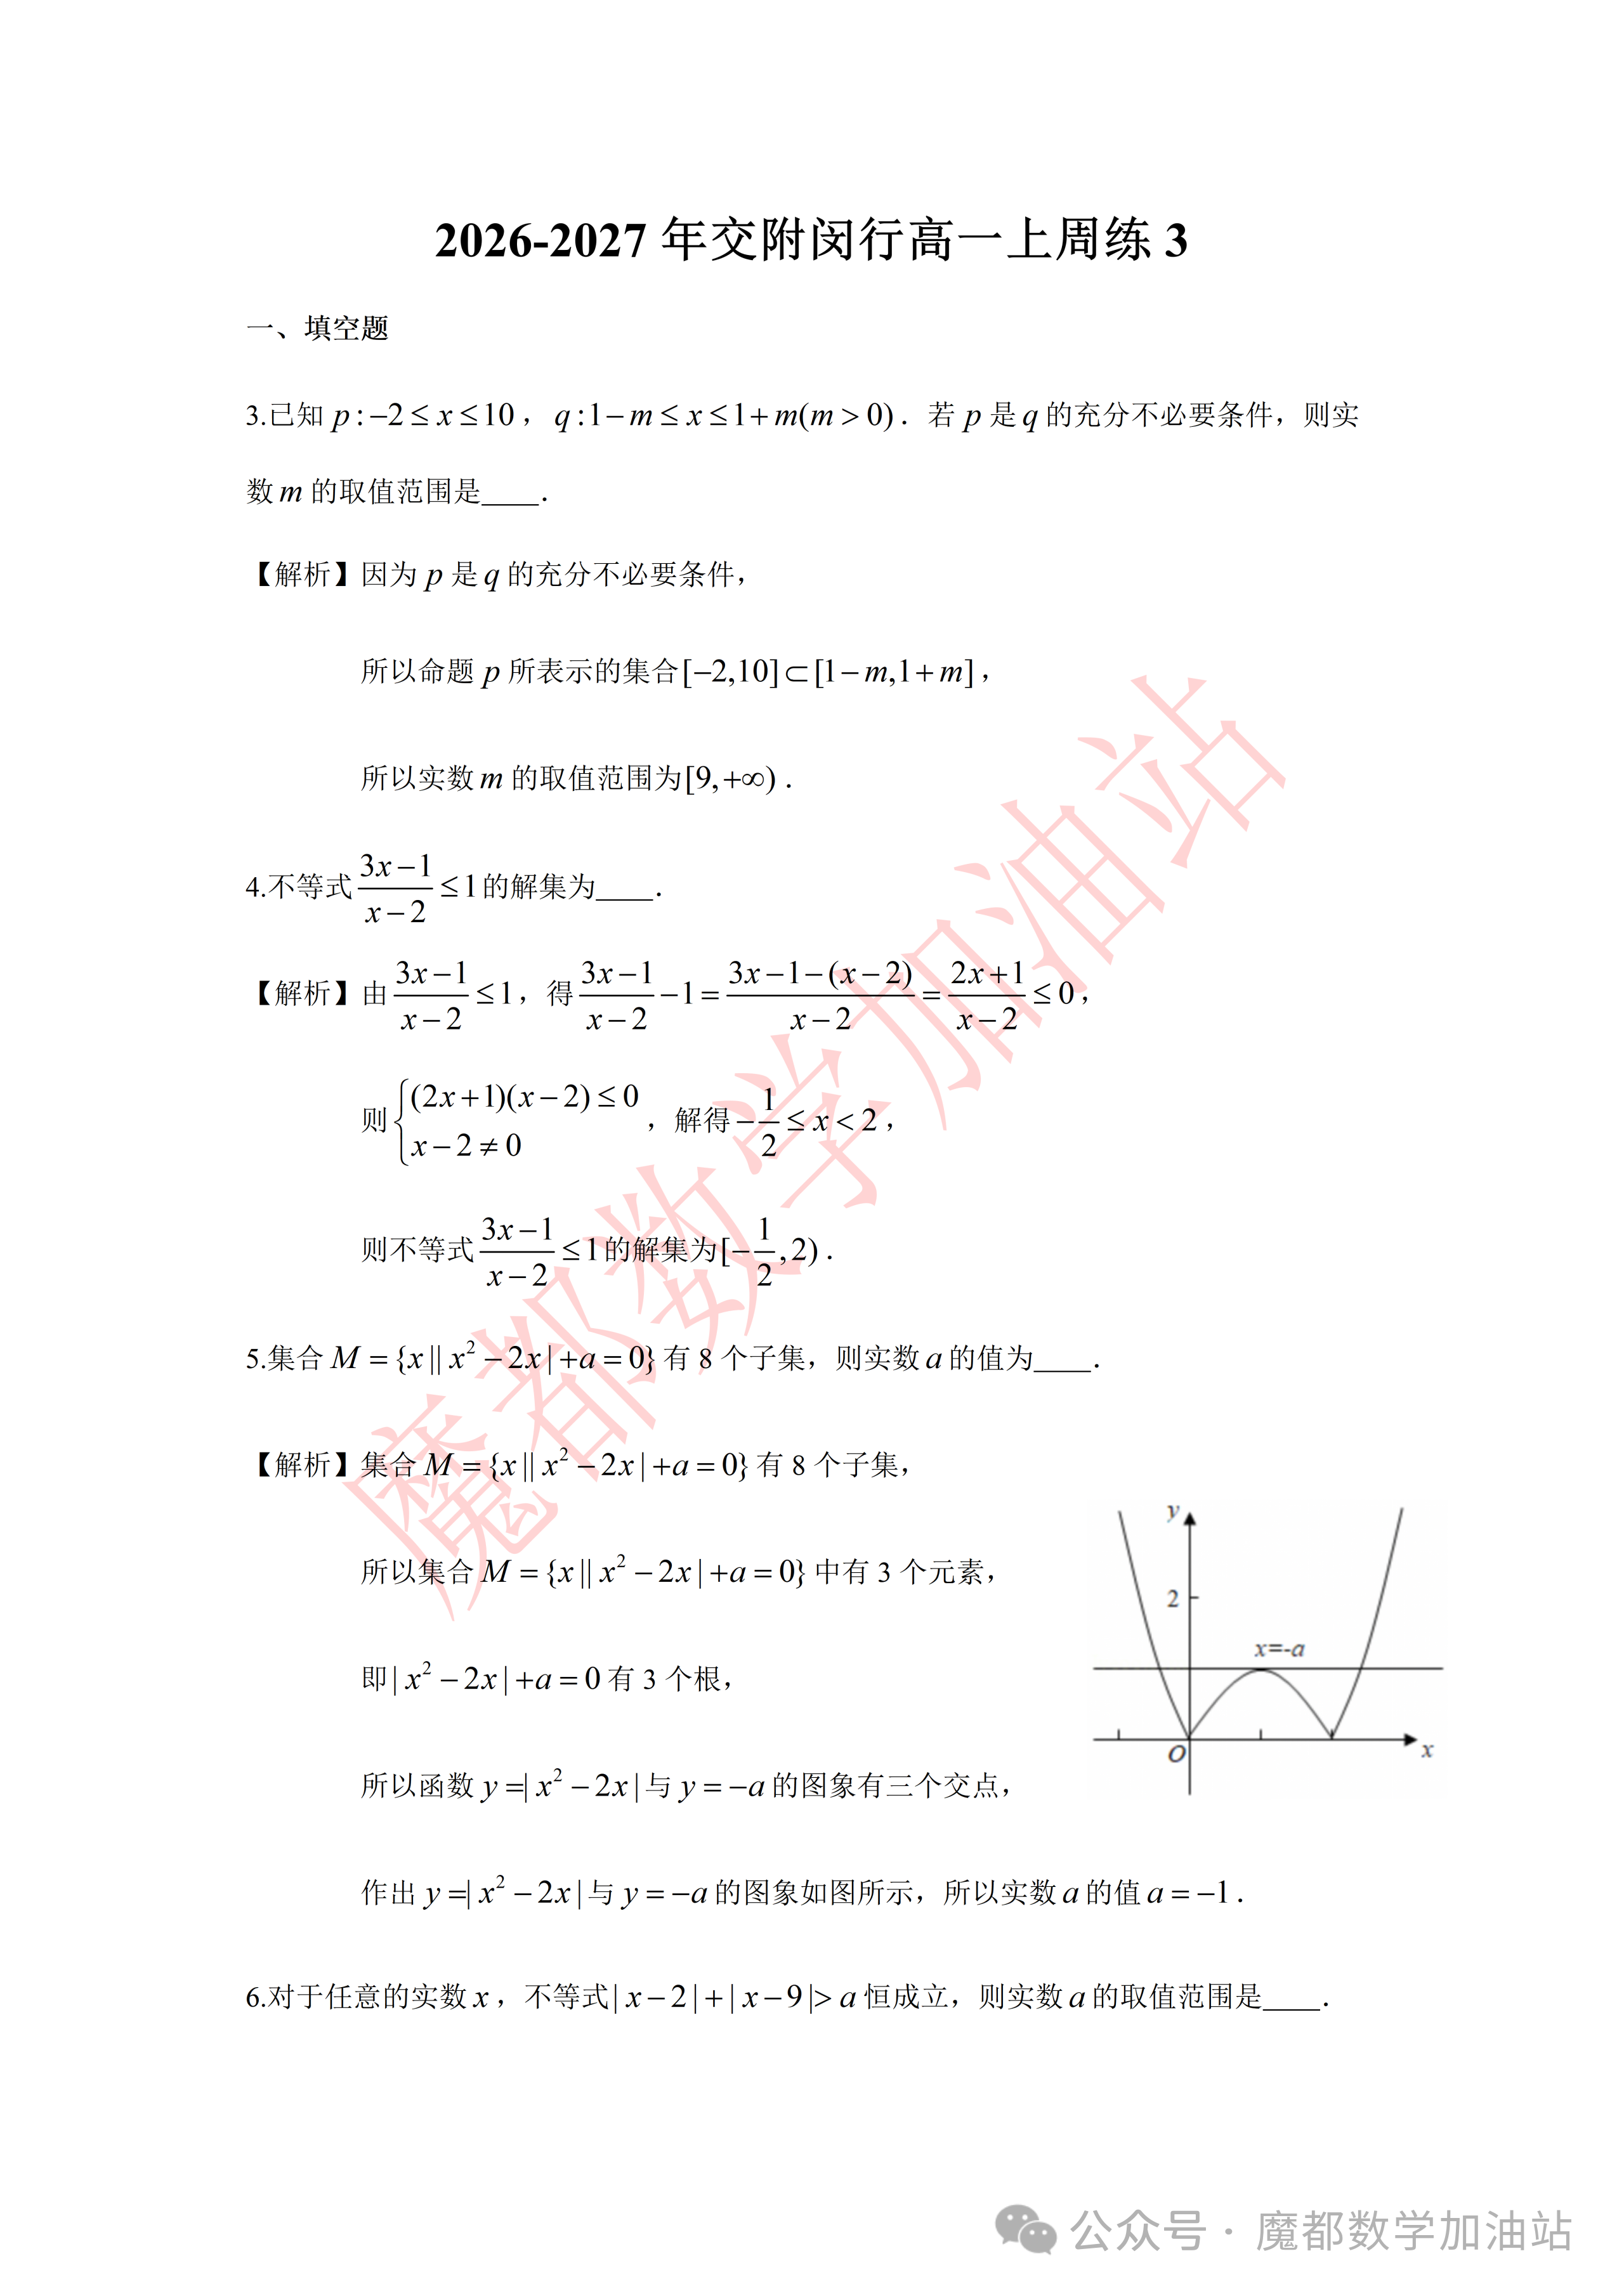
\includegraphics[width=0.14\textwidth,trim={1721bp 837bp 280bp 2297bp},clip]{../原图/高一43_交附闵行_周练3/01.png}
\end{center}

\solbegin
\step{集合 $M=\{x\mid |x^2-2x|+a=0\}$ 有 8 个子集，}
\step{所以集合 $M=\{x\mid |x^2-2x|+a=0\}$ 中有 3 个元素，}
\step{即 $|x^2-2x|+a=0$ 有 3 个根，}
\step{所以函数 $y=|x^2-2x|$ 与 $y=-a$ 的图象有三个交点，}
\step{作出 $y=|x^2-2x|$ 与 $y=-a$ 的图象如图所示，所以实数 $a$ 的值 $a=-1$.}
\solend

\fi

\item 对于任意的实数 $x$，不等式 $|x-2|+|x-9|>a$ 恒成立，则实数 $a$ 的取值范围是 \blankline[4.4em].

\ifanswer
\solbegin
\step{由绝对值的几何意义得 $|x-2|+|x-9|\geqslant7$，当且仅当 $2\leqslant x\leqslant9$ 时等号成立，}
\step{所以 $a<7$，}
\step{即 $a$ 的取值范围为 $(-\infty,7)$.}
\solend

\fi

\item 已知集合 $A=\{x\mid(a-1)x^2+3x-2=0\}$，$B=\{x\mid x^2-3x+2=0\}$，$A\subseteq B$，求实数 $a$ 的取值范围是 \blankline[4.4em].

\ifanswer
\solbegin
\step{由方程 $x^2-3x+2=0$，解得 $x=1$ 或 $x=2$，即 $B=\{1,2\}$，}
\step{因为 $A\subseteq B$，所以 $A=\varnothing$ 或 $A=\{1\}$ 或 $A=\{2\}$ 或 $A=\{1,2\}$，}
\step{当 $A=\varnothing$ 时，$a\neq1$，且 $\Delta=3^2-4(a-1)\times(-2)<0$，解得 $a<-\dfrac18$，}
\step{将 $x=1$ 代入方程 $(a-1)x^2+3x-2=0$，得 $a=0$，}
\step{此时 $A=\{x\mid-x^2+3x-2=0\}=\{1,2\}$，满足条件，}
\step{将 $x=2$ 代入方程 $(a-1)x^2+3x-2=0$，得到 $a=0$，上面已经验证满足条件，}
\step{综上所述，$a$ 的取值范围是 $\left(-\infty,-\dfrac18\right)\cup\{0\}$.}
\solend

\fi

\item 已知 $a$、$b$、$c$、$d$ 为常数，若不等式
$\dfrac{b}{x+a}+\dfrac{x+d}{x+c}<0$ 的解集为 $\left(-1,-\dfrac13\right)\cup\left(\dfrac12,1\right)$，
则不等式 $\dfrac{bx}{ax-1}+\dfrac{dx-1}{cx-1}<0$ 的解集为 \blankline[4.4em].

\ifanswer
\solbegin
\step{若 $x=0$，原不等式化为 $1<0$，不等式显然不成立，所以 $x\neq0$，}
\step{由 $\dfrac{bx}{ax-1}+\dfrac{dx-1}{cx-1}<0$，得 $\dfrac{b}{a-\dfrac1x}+\dfrac{d-\dfrac1x}{c-\dfrac1x}<0$，即 $\dfrac{b}{-\dfrac1x+a}+\dfrac{-\dfrac1x+d}{-\dfrac1x+c}<0$.}
\step{因为不等式 $\dfrac{b}{x+a}+\dfrac{x+d}{x+c}<0$ 的解集为 $\left(-1,-\dfrac13\right)\cup\left(\dfrac12,1\right)$，}
\step{所以 $-1<-\dfrac1x<-\dfrac13$ 或 $\dfrac12<-\dfrac1x<1$，解得 $1<x<3$ 或 $-2<x<-1$，}
\step{所以不等式 $\dfrac{bx}{ax-1}+\dfrac{dx-1}{cx-1}<0$ 的解集为 $(-2,-1)\cup(1,3)$.}
\solend

\fi

\item 正实数 $x$、$y$ 满足 $2x+3y-xy=0$，且存在这样的 $x$、$y$ 使不等式 $x+y<m+1$ 有解，则实数 $m$ 的取值范围是 \blankline[4.4em].

\ifanswer
\solbegin
\step{因为正实数 $x$、$y$ 满足 $2x+3y-xy=0$，则 $\dfrac2y+\dfrac3x=1$，$x>0$，$y>0$，}
\step{所以 $x+y=(x+y)\left(\dfrac3x+\dfrac2y\right)=3+\dfrac{2x}{y}+\dfrac{3y}{x}+2\geqslant2\sqrt{\dfrac{2x}{y}\times\dfrac{3y}{x}}+5=5+2\sqrt6$，}
\step{当且仅当 $\sqrt2x=\sqrt3y$ 时取等号，}
\step{存在这样的 $x$、$y$ 使不等式 $x+y<m+1$ 有解，则 $m+1>5+2\sqrt6$，}
\step{则 $m>4+2\sqrt6$，所以实数 $m$ 的取值范围是 $(4+2\sqrt6,+\infty)$.}
\solend

\fi

\item 若 $a$、$b$、$c\in\R$，$a^2+b^2+c^2=1$，则 $2ab+bc$ 的最大值为 \blankline[4.4em].

\ifanswer
\solbegin
\step{对于 $2ab+bc$，将 $b^2$ 拆分为 $\dfrac45b^2+\dfrac15b^2$，则 $a^2+\dfrac45b^2+c^2+\dfrac15b^2=1$，}
\step{$a^2+\dfrac45b^2\geqslant2\cdot a\cdot\dfrac2{\sqrt5}b=\dfrac4{\sqrt5}ab$，$c^2+\dfrac15b^2\geqslant2\cdot c\cdot\dfrac1{\sqrt5}b=\dfrac2{\sqrt5}bc$，}
\step{两式相加得 $1\geqslant\dfrac4{\sqrt5}ab+\dfrac2{\sqrt5}bc=\dfrac2{\sqrt5}(2ab+bc)$，故 $2ab+bc\leqslant\dfrac{\sqrt5}2$，}
\step{等号成立当且仅当 $a=\dfrac2{\sqrt5}b$，$c=\dfrac1{\sqrt5}b$，}
\step{代入 $a^2+b^2+c^2=1$，得 $\dfrac45b^2+b^2+\dfrac15b^2=2b^2=1$，即 $b=\dfrac{\sqrt2}2$，}
\step{此时 $a=\dfrac{\sqrt{10}}5$，$c=\dfrac{\sqrt{10}}{10}$，故 $2ab+bc$ 的最大值为 $\dfrac{\sqrt5}2$.}
\solend

\fi

\item 已知实数 $a$、$b$ 满足 $-3<a+2b<2$，$-1<2a-b<4$，则 $a+b$ 的取值范围为 \blankline[4.4em].

\ifanswer
\solbegin
\step{设 $a+b=m(a+2b)+n(2a-b)=(m+2n)a+(2m-n)b$，}
\step{所以 $\begin{cases}m+2n=1\\2m-n=1\end{cases}$，解得 $n=\dfrac15$，$m=\dfrac35$，所以 $a+b=\dfrac35(a+2b)+\dfrac15(2a-b)$，}
\step{因为 $-3<a+2b<2$，$-1<2a-b<4$，}
\step{所以 $-\dfrac95<\dfrac35(a+2b)<\dfrac65$，$-\dfrac15<\dfrac15(2a-b)<\dfrac45$，}
\step{相加得 $-2<\dfrac35(a+2b)+\dfrac15(2a-b)<2$，即 $-2<a+b<2$，}
\step{故 $a+b$ 的取值范围为 $(-2,2)$.}
\solend

\fi

% 注：原卷题干与解析均印作 \sqrt{2xyz}，但按其自身答案 8 与取等值（$y=\dfrac12$，
% $x=\dfrac{\sqrt3}4$，$z=\dfrac{\sqrt6}4$）代入只与 $\sqrt{2x^2y^2z^2}=\sqrt2\,xyz$ 相符，
% $\sqrt{2xyz}$ 与答案 8 不自洽，原卷如此，照录未改。
\item 已知正数 $x$、$y$、$z$ 满足 $2x^2+y^2+z^2=1$，则 $\dfrac{y+1}{\sqrt{2xyz}}$ 的最小值为 \blankline[4.4em].

\ifanswer
\solbegin
\step{由条件得 $2x^2+z^2=1-y^2=(1-y)(1+y)$，则 $1+y=\dfrac{2x^2+z^2}{1-y}$，}
\step{结合 $x$、$y$、$z>0$ 得原式 $=\dfrac{2x^2+z^2}{\sqrt{2xyz}(1-y)}\geqslant\dfrac{2\sqrt2xz}{\sqrt{2xyz}(1-y)}=\dfrac2{y(1-y)}$，}
\step{又 $y(1-y)\leqslant\left(\dfrac{y+1-y}2\right)^2=\dfrac14$，所以 $\dfrac2{y(1-y)}\geqslant\dfrac2{\frac14}=8$，}
\step{当且仅当 $\sqrt2x=z$，且 $y=1-y$，即 $y=\dfrac12$，$x=\dfrac{\sqrt3}4$，$z=\dfrac{\sqrt6}4$ 时取等号，}
\step{故 $\dfrac{y+1}{\sqrt{2xyz}}$ 最小值为 $8$.}
\solend

\fi

\end{enumerate}

\bigsec{二、选择题}

\begin{enumerate}
\setcounter{enumi}{12}

\item 已知关于 $x$ 的方程 $(1-k)x^2-2x-1=0$ 有实数根，则 $k$ 的取值范围是\mbox{（\quad）}

\keepwithprev
A. $k\leqslant2$ 且 $k\neq1$\qquad B. $k\leqslant2$\qquad
C. $k<2$ 且 $k\neq1$\qquad D. $k<2$

\ans{$A$}

\ifanswer
\solbegin
\step{由题意得 $\begin{cases}1-k\neq0\\\Delta=4+4(1-k)\geqslant0\end{cases}$，解不等式得 $\begin{cases}1\neq k\\2-k>0\end{cases}$，所以 $k\leqslant2$ 且 $k\neq1$，}
\step{故选 $A$.}
\solend

\fi

\item 不等式 $2|x+2|+|x-1|\geqslant5$ 成立的一个必要不充分条件是\mbox{（\quad）}

\keepwithprev
A. $x\leqslant-1$ 或 $x\geqslant0$\qquad B. $x\geqslant0$

C. $x\leqslant-\dfrac83$ 或 $x\geqslant0$\qquad D. $x\geqslant1$

\ans{$A$}

\ifanswer
\solbegin
\step{当 $x<-2$ 时，原不等式可化为 $-2x-4-x+1\geqslant5$，解得 $x\leqslant-\dfrac83$，}
\step{当 $-2\leqslant x<1$ 时，原不等式可化为 $2x+4-x+1\geqslant5$，解得 $0\leqslant x<1$，}
\step{当 $x\geqslant1$ 时，原不等式可化为 $2x+4+x-1\geqslant5$，解得 $x\geqslant\dfrac23$，得 $x\geqslant1$，}
\step{综上所述，不等式 $2|x+2|+|x-1|\geqslant5$ 成立的充要条件是 $x\leqslant-\dfrac83$ 或 $x\geqslant0$，}
\step{设 $A=\{x\mid x\leqslant-\dfrac83\text{ 或 }x\geqslant0\}$，}
\step{则不等式 $2|x+2|+|x-1|\geqslant5$ 成立的必要不充分条件，}
\step{其对应的集合 $B$ 满足 $A\subsetneq B$，对照各个选项，$A$ 项符合题意. 故选 $A$.}
\solend

\fi

\item 已知实数 $a>0$，$b>0$，$\dfrac1{a+1}+\dfrac1{b+1}=1$，则 $2a+3b$ 的最小值为\mbox{（\quad）}

\keepwithprev
A. $2\sqrt6$\qquad B. $3+2\sqrt6$\qquad
C. $5+2\sqrt6$\qquad D. $3+2\sqrt2$

\ans{$A$}

\ifanswer
\solbegin
\step{因为 $a>0$，$b>0$，$\dfrac1{a+1}+\dfrac1{b+1}=1$，}
\step{所以 $2a+3b=2(a+1)+3(b+1)-5=[2(a+1)+3(b+1)]\cdot\left(\dfrac1{a+1}+\dfrac1{b+1}\right)-5$}
\step{$=\left[2+3+\dfrac{3(b+1)}{a+1}+\dfrac{2(a+1)}{b+1}\right]-5\geqslant5+2\sqrt{\dfrac{3(b+1)}{a+1}\times\dfrac{2(a+1)}{b+1}}-5=2\sqrt6$，}
\step{当且仅当 $\dfrac{3(b+1)}{a+1}=\dfrac{2(a+1)}{b+1}$，即 $a=\dfrac{\sqrt6}2$，$b=\dfrac{\sqrt6}3$ 时取等号. 故选 $A$.}
\solend

\fi

\item 已知集合 $U=\{n\mid1\leqslant n\leqslant2027,\ n\in\N\}$，集合 $M\subseteq U$，若对于 $M$ 中任意两个不同的元素 $x$ 和 $y$，都有 $|x-y|>2$，则 $M$ 中元素个数的最大值是\mbox{（\quad）}

\keepwithprev
A. $676$\qquad B. $675$\qquad C. $672$\qquad D. $671$

\ans{$A$}

\ifanswer
\solbegin
\step{对于 $M$ 中的任意两个不同的元素 $x$、$y$，都有 $|x-y|>2$，}
\step{不妨设 $x>y$，都有 $x-y\geqslant3$，}
\step{要想 $M$ 所含元素个数最大，则要 $x-y$ 尽可能小，故需使得 $x-y$ 的最小值为 3，}
\step{将 $1\sim2027$ 这 2027 个元素按如下分组：}
\step{$\{1,2,3\}$，$\{4,5,6\}$，$\cdots$，$\{2023,2024,2025\}$，$\{2026,2027\}$，}
\step{故应在前 675 组中按周期 3 每组取一个元素，且第一组中不能取 3，}
\step{第一组中取 1 时，得 $M=\{1,4,7,\cdots,2023,2026\}$，}
\step{或 $M=\{1,4,7,\cdots,2023,2027\}$ 这样的集合，}
\step{第一组取 2 时，得 $M=\{2,5,8,\cdots,2024,2027\}$，}
\step{其中任意两元素差值 $x-y$（$x>y$）都大于 2，满足题意，}
\step{故 $M$ 所含元素个数的最大值为 $\dfrac{2025}{3}+1=676$. 故选 $A$.}
\solend

\fi

\end{enumerate}

\bigsec{三、解答题}

\begin{enumerate}
\setcounter{enumi}{16}

\item 已知 $a\in\R$，集合 $A=\left\{x\middle|\dfrac{2-x}{x+1}\leqslant0\right\}$，$B=\{x\mid x^2+(3-a)x-3a<0\}$.

\begin{enumerate}[label=(\arabic*)]
\item 当 $a=\dfrac13$ 时，求 $A$ 和 $B$；
\item 已知 $A\cup B=A$，求实数 $a$ 的取值范围.
\end{enumerate}

\ifanswer
\solbegin
\stepm{(1)}{由 $\dfrac{2-x}{x+1}\leqslant0$，得 $\begin{cases}(2-x)(x+1)\leqslant0\\x\neq-1\end{cases}$，解得 $x<-1$ 或 $x\geqslant2$，}
\step{则 $A=\{x\mid x<-1\text{ 或 }x\geqslant2\}$；}
\step{$B=\{x\mid x^2+(3-a)x-3a<0\}=\{x\mid(x+3)(x-a)<0\}$，}
% 注：原卷此行印作 $(x+2)\left(x-\dfrac13\right)$，按前一行 $B=\{x\mid(x+3)(x-a)<0\}$ 应为
% $(x+3)\left(x-\dfrac13\right)$，原卷如此，照录未改。
\step{当 $a=\dfrac13$ 时，$B=\left\{x\middle|(x+2)\left(x-\dfrac13\right)<0\right\}$，}
\step{解得 $B=\left\{x\middle|-3<x<\dfrac13\right\}$.}
\stepm{(2)}{由 $A\cup B=A$，得 $B\subseteq A$，}
\step{①当 $B=\varnothing$ 时，得 $a=-3$，符合题意；}
\step{②当 $B\neq\varnothing$ 时，若 $a>-3$，则 $B=\{x\mid-3<x<a\}$，}
\step{由 $B\subseteq A$，得 $a\leqslant-1$，此时 $-3<a\leqslant-1$；}
\step{若 $a<-3$，则 $B=\{x\mid a<x<-3\}$，此时 $B\subseteq A$ 恒成立，}
\step{故 $a<-3$ 符合题意；}
\step{综上所述，实数 $a$ 的取值范围为 $a\leqslant-1$.}
\solend

\fi

\ansspace[6]

\item 甲乙两地的高速公路全长 166 千米，汽车从甲地进入该高速公路后匀速行驶到乙地，车速 $v\in[70,120]$（千米/时）. 已知汽车每小时的运输成本（以元为单位）由可变部分和固定部分组成：可变部分为 $0.02v^2$，固定部分为 220 元.

\begin{enumerate}[label=(\arabic*)]
\item 若每小时的运输成本不高于 420 元，汽车的速度应该控制在什么范围？
\item 汽车应以多大速度行驶才能使全程运输成本最小？最小运输成本约为多少元？（结果保留整数）
\end{enumerate}

\ifanswer
\solbegin
\stepm{(1)}{已知汽车每小时的运输成本（以元为单位）由可变部分和固定部分组成：}
\step{可变部分为 $0.02v^2$，固定部分为 220 元，}
\step{则汽车每小时的运输成本为 $0.02v^2+220$（元），}
\step{若每小时的运输成本不高于 420 元，}
\step{则 $0.02v^2+220\leqslant420$，解得 $v^2\leqslant10000$，}
\step{得 $70\leqslant v\leqslant100$，即 $v\in[70,100]$（千米/时），}
\step{则此时汽车的速度 $v$ 应该控制在 $[70,100]$（千米/时）；}
\stepm{(2)}{因为汽车从甲地进入该高速公路后匀速行驶到乙地，}
\step{车速 $v\in[70,120]$（千米/时），所以汽车的行驶时间为 $\dfrac{166}{v}$（小时），}
\step{所以全程运输成本 $y=\dfrac{166}{v}(0.02v^2+220)=3.32v+\dfrac{36520}{v}$，}
% 注：原卷此行印作 $v\in[70,100]$，与题干的 $v\in[70,120]$ 不自洽（若 $v\in[70,100]$，
% 最小值应在 $v=100$ 处取得，与下文 $v=10\sqrt{110}\approx105$ 矛盾），原卷如此，照录未改。
\step{$v\in[70,100]$，}
\step{由基本不等式得 $y=3.32v+\dfrac{36520}{v}\geqslant2\sqrt{3.32v\times\dfrac{36520}{v}}\approx696$，}
\step{当且仅当 $3.32v=\dfrac{36520}{v}$，即 $v=10\sqrt{110}\approx105$ 时取等号，}
\step{汽车应以 105（千米/时）行驶才能使全程运输成本最小，}
\step{最小运输成本约为 696 元.}
\solend

\fi

\ansspace[8]

\item
\begin{enumerate}[label=(\arabic*)]
\item 已知 $a$、$b$、$c$ 为实数，求证：$|a-b|\leqslant|a-c|+|b-c|$，并说明等号成立的条件；
\item 设 $x\in\R$，求方程 $|3x-8|=|5-x|+|2x-3|$ 的解集.
\end{enumerate}

\ifanswer
% 注：原卷第 19 题未印【解析】，仅印一行【答案】"（1）(a-c)(b-c)≤0；
% （2）(-∞,3/2]∪[5,+∞)"。(1) 的两行推导为本稿所补，(2) 照录原卷答案。
% 又题干作"方程"，而所给答案 (-∞,3/2]∪[5,+∞) 实为不等式 |3x-8|≤|5-x|+|2x-3| 的解集，
% 与"方程"不合，原卷如此，照录未改。
\solbegin
\stepm{(1)}{由三角不等式 $|a-b|=|(a-c)-(b-c)|\leqslant|a-c|+|b-c|$，}
\step{当且仅当 $(a-c)(b-c)\leqslant0$ 时等号成立.}
\stepm{(2)}{$\left(-\infty,\dfrac32\right]\cup[5,+\infty)$.}
\solend

\fi

\ansspace[6]

\item 已知正实数 $a$、$b$ 满足 $a+b=1$，求 $\dfrac1a+\dfrac1b$ 的最小值. 其中一种解法是：

\[
\begin{aligned}
\dfrac1a+\dfrac1b
&=\left(\dfrac1a+\dfrac1b\right)(a+b)\\
&=1+\dfrac ba+\dfrac ab+1\\
&\geqslant2+2\sqrt{\dfrac ba\times\dfrac ab}=2+2=4.
\end{aligned}
\]
当且仅当 $\dfrac ba=\dfrac ab$ 且 $a+b=1$ 时即 $a=b=\dfrac12$ 时取等号.
学习上述解法并解决下列问题：

\begin{enumerate}[label=(\arabic*)]
\item 若正实数 $x$、$y$ 满足 $x+y=xy$，求 $2x+y$ 的最小值；
\item 若实数 $a$、$b$、$x$、$y$ 满足 $\dfrac{x^2}{a^2}+\dfrac{y^2}{b^2}=1$，求证：$a^2+b^2\geqslant(x+y)^2$；
\item 求代数式 $M=\sqrt{m-1}+\sqrt{3-m}$ 的最大值，并求出使得 $M$ 最大的 $m$ 的值.
\end{enumerate}

\ifanswer
\solbegin
\stepm{(1)}{因为正实数 $x$、$y$ 满足 $x+y=xy$，$\dfrac{x+y}{xy}=1\Rightarrow\dfrac1y+\dfrac1x=1$，}
\step{所以 $(2x+y)\times1=(2x+y)\left(\dfrac1y+\dfrac1x\right)=3+\dfrac{2x}{y}+\dfrac yx\geqslant3+2\sqrt{\dfrac{2x}{y}\cdot\dfrac yx}=3+2\sqrt2$，}
\step{当且仅当 $\dfrac{2x}{y}=\dfrac yx$ 且 $\dfrac1y+\dfrac1x=1$ 时取等号，}
\step{解得 $x=\dfrac{2+\sqrt2}2$，$y=\sqrt2x=\sqrt2\times\dfrac{2+\sqrt2}2=1+\sqrt2$，}
\step{所以 $2x+y$ 的最小值为 $3+2\sqrt2$；}
\stepm{(2)}{因为 $\dfrac{x^2}{a^2}+\dfrac{y^2}{b^2}=1$，}
\step{所以 $a^2+b^2=(a^2+b^2)\left(\dfrac{x^2}{a^2}+\dfrac{y^2}{b^2}\right)=x^2+y^2+\dfrac{b^2x^2}{a^2}+\dfrac{a^2y^2}{b^2}$，}
\step{因为 $\dfrac{b^2x^2}{a^2}+\dfrac{a^2y^2}{b^2}\geqslant2\sqrt{\dfrac{b^2x^2}{a^2}\times\dfrac{a^2y^2}{b^2}}=2\sqrt{x^2y^2}=2|xy|$，}
\step{当且仅当 $\dfrac{b^2x^2}{a^2}=\dfrac{a^2y^2}{b^2}$ 时取等号，}
\step{所以 $x^2+y^2+\dfrac{b^2x^2}{a^2}+\dfrac{a^2y^2}{b^2}\geqslant x^2+y^2+2|xy|\geqslant x^2+y^2+2xy=(x+y)^2$，}
\step{所以 $a^2+b^2\geqslant(x+y)^2$；}
\stepm{(3)}{因为 $M=\sqrt{m-1}+\sqrt{3-m}$，所以 $\begin{cases}m-1\geqslant0\\3-m\geqslant0\end{cases}$，解得 $1\leqslant m\leqslant3$，}
\step{所以 $M^2=(\sqrt{m-1}+\sqrt{3-m})^2=2+2\sqrt{(3-m)(m-1)}$，}
\step{由基本不等式得 $(3-m)(m-1)\leqslant\left(\dfrac{(3-m)+(m-1)}2\right)^2=1$，}
\step{当且仅当 $3-m=m-1$ 时取等号，解得 $m=2$，}
\step{所以 $M^2=2+2\sqrt{(3-m)(m-1)}\leqslant2+2\sqrt1=4$，}
\step{因为 $M>0$，所以 $M\leqslant2$，所以 $M$ 最大值为 2，此时 $m$ 的值为 2.}
\solend

\fi

\ansspace[8]

\item 若有限个正整数组成的集合 $A$ 中至少有两个元素，且对于任意的 $x,y\in A$（$x>y$），都有 $\dfrac{y^2}{x-y}\in A$，则称 $A$ 为“L-集合”.

\begin{enumerate}[label=(\arabic*)]
\item 判断 $\{1,2,4\}$ 是否为“L-集合”，说明理由；
\item 若双元素集 $M$ 为“L-集合”，且 $4\in M$，求所有满足条件的集合 $M$；
\item 求所有满足条件的“L-集合”.
\end{enumerate}

\ifanswer
\solbegin
\stepm{(1)}{若至少由两个元素构成的有限集合 $A\subseteq\N^*$，}
% 注：原卷下一行"都有"后未印分数 \dfrac{y^2}{x-y}，径作"都有 A"，原卷如此，照录未改。
\step{且对于任意的 $x$、$y\in A$（$x>y$），都有 $A$，则称 $A$ 为“L-集合”，}
\step{$\{1,2,4\}$ 不为“L-集合”，理由如下：}
\step{因为 $\dfrac{1^2}{4-1}=\dfrac13\notin\{1,2,4\}$，所以 $\{1,2,4\}$ 不是“L-集合”.}
\stepm{(2)}{设 $M=\{4,m\}$（$m\in\N^*$，$m\neq4$），}
\step{若 $m<4$，则 $\dfrac{m^2}{4-m}=m$ 或 $\dfrac{m^2}{4-m}=4$，}
\step{由 $\dfrac{m^2}{4-m}=m$，解得 $m=2$，$m=0$（舍去），此时 $M=\{2,4\}$；}
\step{由 $\dfrac{m^2}{4-m}=4$ 化为 $m^2+4m-16=0$，而 $\Delta=4^2+4\times16=80$，}
\step{故方程无正整数解.}
\step{若 $m>4$，则 $\dfrac{4^2}{m-4}=4$ 或 $\dfrac{4^2}{m-4}=m$，}
\step{由 $\dfrac{4^2}{m-4}=4$，解得 $m=8$，此时 $M=\{4,8\}$；}
\step{由 $\dfrac{4^2}{m-4}=m$ 化为 $m^2-4m-16=0$，而 $\Delta=4^2+4\times16=80$，}
\step{故方程无正整数解.}
\step{综上，双元素集 $M$ 为“L-集合”，且 $4\in M$，}
\step{则所有满足条件的集合 $M$ 为 $\{4,8\}$，$\{2,4\}$.}
\stepm{(3)}{若“L-集合”为双元素集，}
\step{不妨设 $M=\{k,m\}$（$k,m\in\N^*$，$m>k$），则 $\dfrac{k^2}{m-k}=k$ 或 $\dfrac{k^2}{m-k}=m$，}
\step{由 $\dfrac{k^2}{m-k}=k$，则 $2k^2=mk$，而 $m>k$，故 $m=2k$，此时 $M=\{k,2k\}$；}
\step{由 $\dfrac{k^2}{m-k}=m$，则 $m^2-mk-k^2=0$，而 $\Delta=5k^2$，显然不存在正整数解；}
\step{所以，“L-集合”为 $\{k,2k\}$，其中 $k\in\N^*$.}
\step{若“L-集合”含有两个以上的元素，}
\step{设最小的元素为 $b$，最大的元素为 $a$，第二大的元素为 $n$，}
\step{则 $\dfrac{b^2}{a-b}$，$\dfrac{n^2}{a-n}$ 是“L-集合”中的元素，}
% 注：原卷下一行未印"由于'L-集合'中的元素均为正整数"一语，径作"若 \dfrac{b^2}{a-b}\geqslant b"，
% 原卷如此，照录未改。
\step{若 $\dfrac{b^2}{a-b}\geqslant b$，解得 $a\leqslant2b$，}
\step{若 $\dfrac{n^2}{a-n}\leqslant n$，则 $a\geqslant2n>2b$，矛盾，}
\step{若 $\dfrac{n^2}{a-n}=a$，该方程的解为 $n=\dfrac{\sqrt5-1}2a$，则 $n$、$a$ 不可能同时为整数，}
\step{无解.}
\step{所以所有满足条件的“L-集合”为 $\{k,2k\}$，其中 $k\in\N^*$.}
\solend

\fi

\ansspace*[10]

\end{enumerate}

\end{document}
"
%
% 原始材料是微信公众号图文（公众号“魔都数学加油站”，作者破晓，2026-10-01 21:37，
% 原文标题“27学年高一43——2026-2027年上海市交附闵行高一上周练3”，
% https://mp.weixin.qq.com/s/-rgkOD9jJVpug6s0uSbwmQ）。正文为 12 张 PNG 页；
% 第 01、05、09、12 页 2560×3620，其余第 02—04、06—08、10—11 页 4762×6735。
% 原文本身是讲评版，题目下方印有解析/答案；题目与讲解照原卷转录，保留原卷错误。
%
% 卷首标题：原卷印作“2026-2027 年交附闵行高一上周练3”，公众号标题中的“上海市”
% 三字不在卷面标题中，本稿依卷面录入；年份区间按全稿惯例排 en dash。
%
% 与原卷的排版差异：
%   ① 原文从第 3 题开始（第 1、2 题未在这篇推文中发布），本稿保留原题号 3—21；
%   ② 原卷本就印有“一、填空题”“二、选择题”“三、解答题”，本稿照原卷分节，
%      改排为全稿统一的大节标题；
%   ③ 原卷未印副标题，本稿按“知识模块”口径补出“集合与常用逻辑用语、不等式”；
%   ④ 原卷填空横线依全稿惯例排为 \blankline[4.4em]；选择题答案只在答案版以 \ans{} 显示，
%      解答区以 \ifanswer 分离；解答题按原卷留出标准作答空间；
%   ⑤ 第 5 题图取自原卷第 1 页截图并裁入本稿，不另建图档；公众号水印不录入。
%      原卷图页分页不保留，正文依本稿版心重新分页。
%
% 原卷存疑/错误（均照录，未改）：
%   ① 第 9 题原卷题干即作"正实数 x、y"，与解析 x>0、y>0 相容，并无矛盾（初稿曾误记
%      题干只称"实数"并据此指原卷不自洽，2026-10-05 回原图核对订正）。
%   ② 第 11 题解析"相加得"一行原卷印作 -2<3/5(a+2b)+1/5(2a-b)<2，第一项系数 3/5
%      原卷不缺（初稿漏抄致该行按字面不成立，2026-10-05 已按原卷补回）。
%   ③ 第 13 题答案印 A，解析以“1-k≠0”排除 k=1；但 k=1 时原方程为 -2x-1=0，
%      仍有实数根，按题意应选 B。本稿保留原卷答案 A 及其解析，不代为订正。
%
\documentclass[a4paper,11pt]{article}
\usepackage{common}
\usepackage{graphicx}

\begin{document}

\examtitlest[3]{2026--2027 年交附闵行高一上周练 3}{集合与常用逻辑用语、不等式}

\bigsec{一、填空题}

\begin{enumerate}
\setcounter{enumi}{2}

\item 已知 $p\colon -2\leqslant x\leqslant10$，$q\colon 1-m\leqslant x\leqslant1+m$（$m>0$）. 若 $p$ 是 $q$ 的充分不必要条件，则实数 $m$ 的取值范围是 \blankline[4.4em].

\ifanswer
\solbegin
\step{因为 $p$ 是 $q$ 的充分不必要条件，}
\step{所以命题 $p$ 所表示的集合 $[-2,10]\subset[1-m,1+m]$，}
\step{所以实数 $m$ 的取值范围为 $[9,+\infty)$.}
\solend

\fi

\item 不等式 $\dfrac{3x-1}{x-2}\leqslant1$ 的解集为 \blankline[4.4em].

\ifanswer
\solbegin
\step{由 $\dfrac{3x-1}{x-2}-1=\dfrac{3x-1-(x-2)}{x-2}=\dfrac{2x+1}{x-2}\leqslant0$，}
\step{则 $\begin{cases}(2x+1)(x-2)\leqslant0\\x-2\neq0\end{cases}$，解得 $-\dfrac12\leqslant x<2$，}
\step{则不等式 $\dfrac{3x-1}{x-2}\leqslant1$ 的解集为 $\left[-\dfrac12,2\right)$.}
\solend

\fi

\item 集合 $M=\{x\mid |x^2-2x|+a=0\}$ 有 8 个子集，则实数 $a$ 的值为 \blankline[4.4em].

\ifanswer
\begin{center}
% 图取自原卷第 1 页；用原图裁切，未重绘。
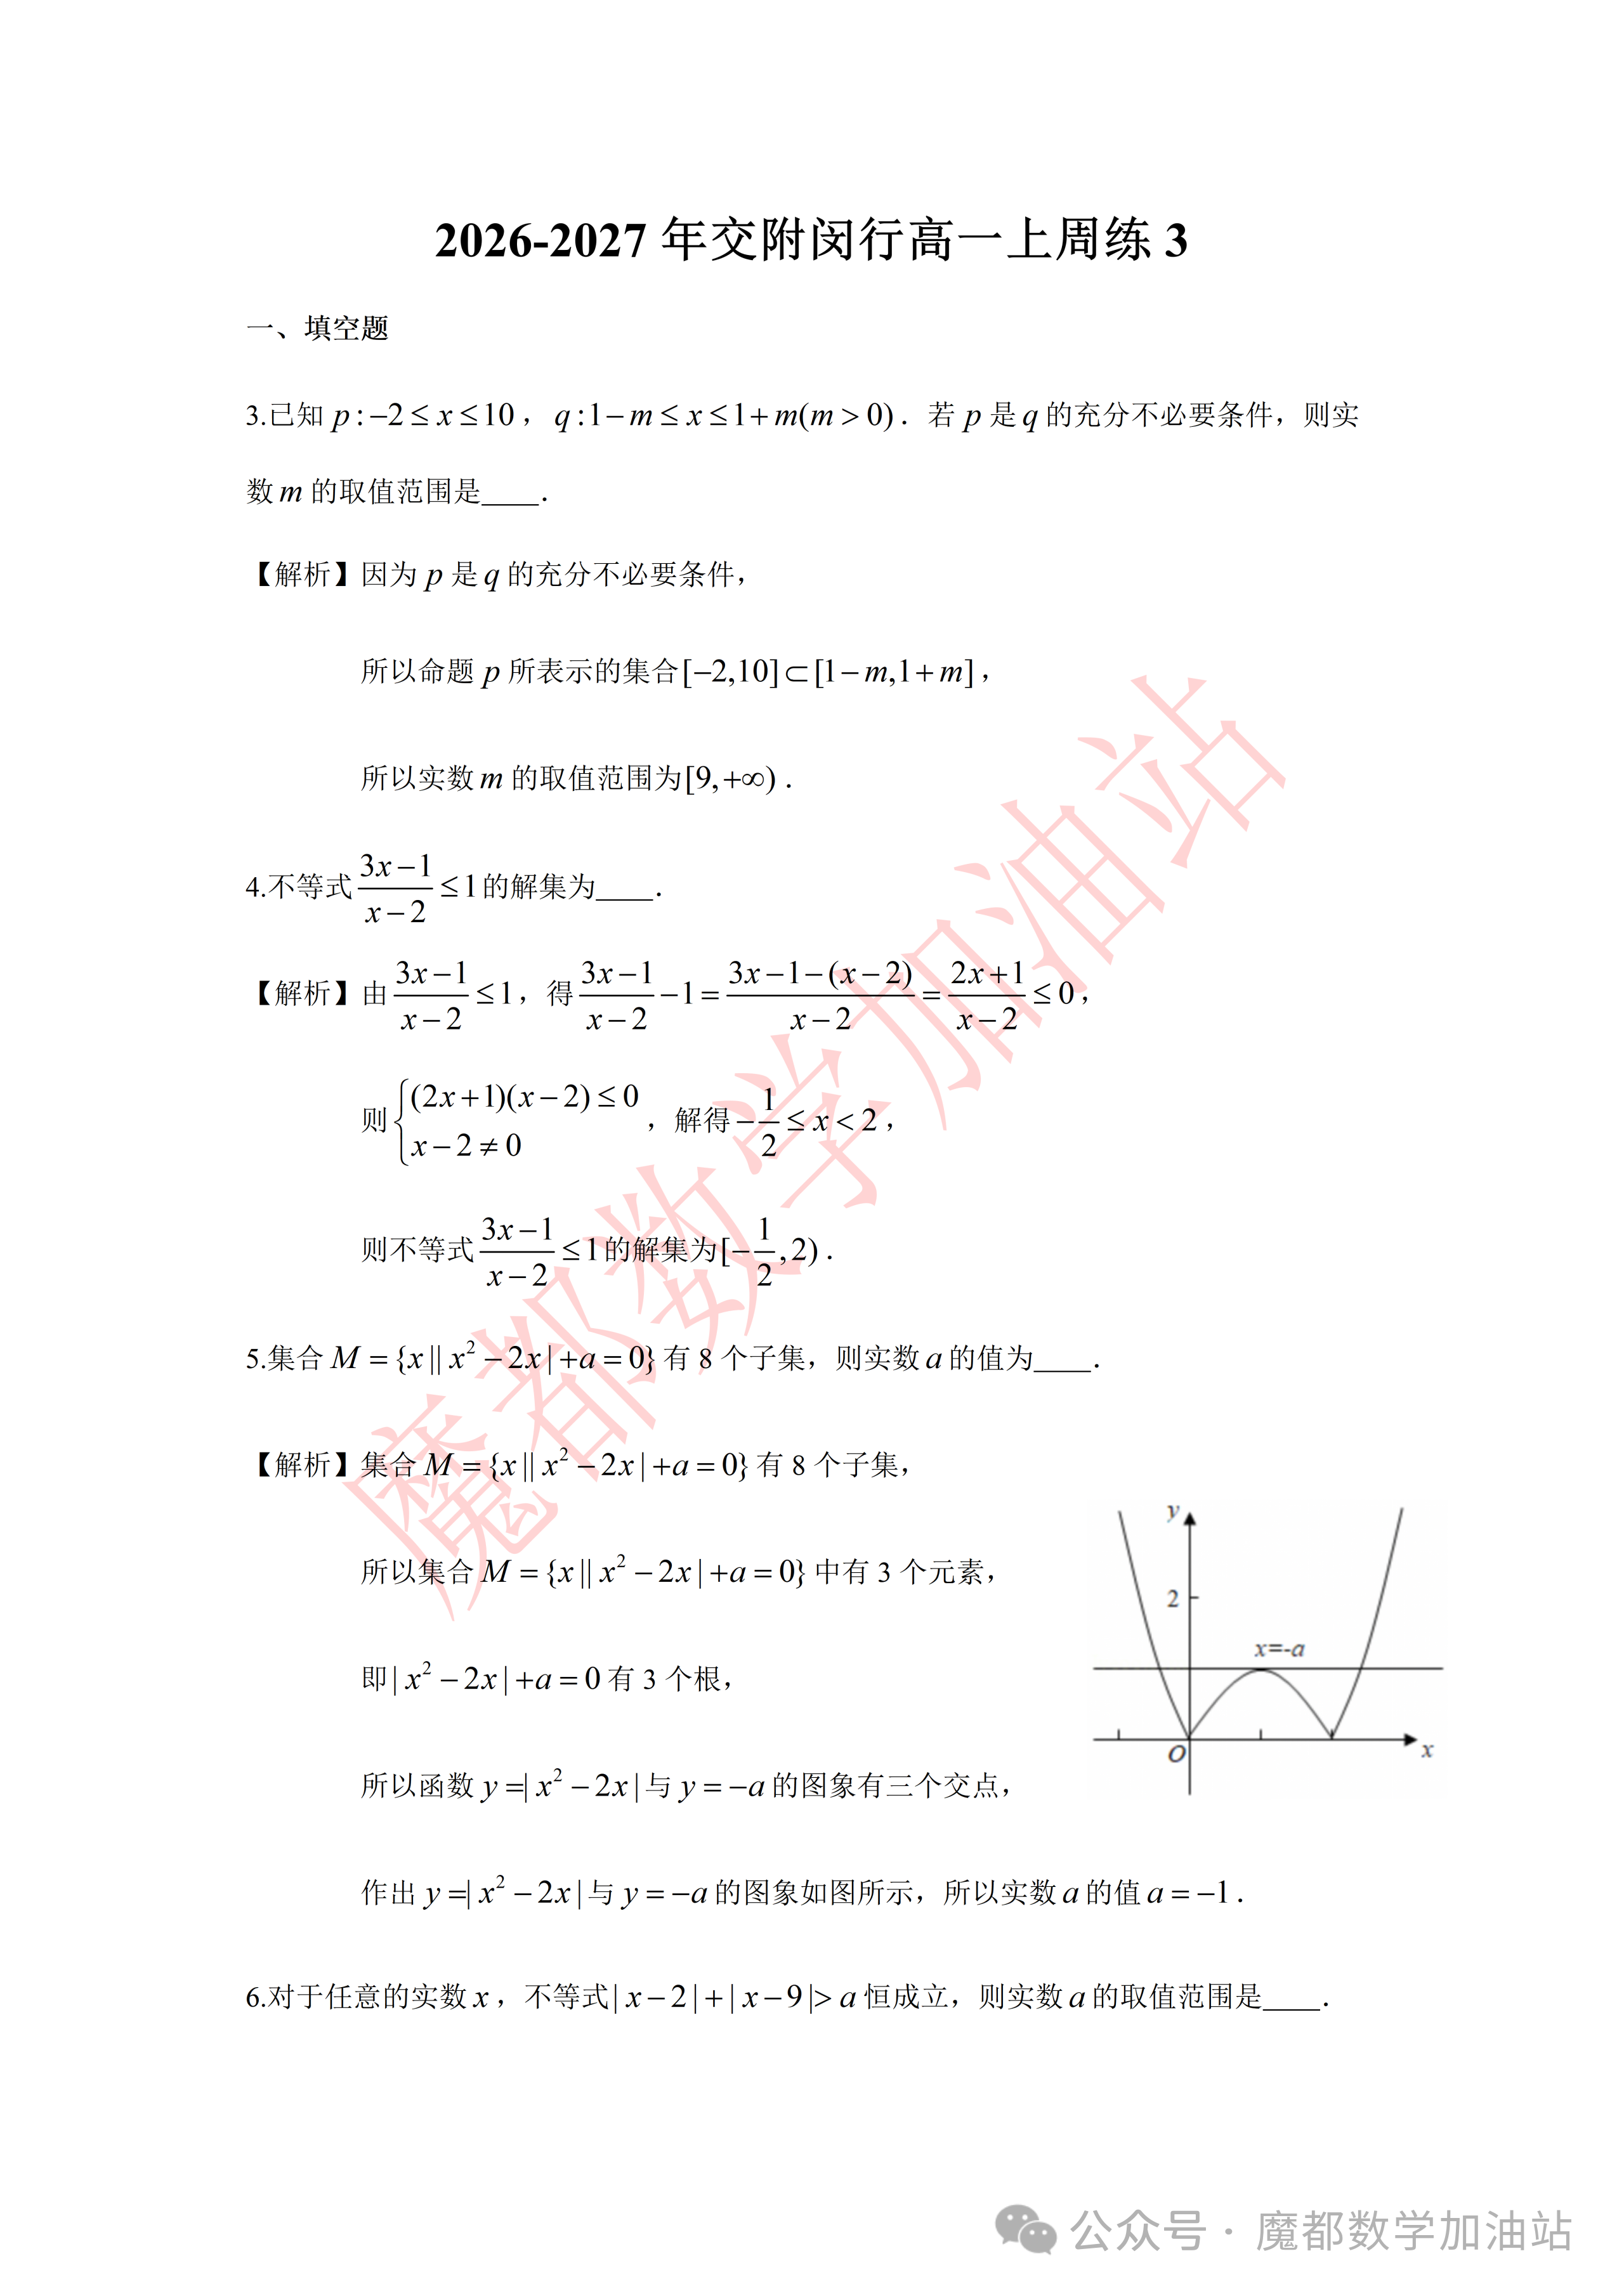
\includegraphics[width=0.14\textwidth,trim={1721bp 837bp 280bp 2297bp},clip]{../原图/高一43_交附闵行_周练3/01.png}
\end{center}

\solbegin
\step{集合 $M=\{x\mid |x^2-2x|+a=0\}$ 有 8 个子集，}
\step{所以集合 $M=\{x\mid |x^2-2x|+a=0\}$ 中有 3 个元素，}
\step{即 $|x^2-2x|+a=0$ 有 3 个根，}
\step{所以函数 $y=|x^2-2x|$ 与 $y=-a$ 的图象有三个交点，}
\step{作出 $y=|x^2-2x|$ 与 $y=-a$ 的图象如图所示，所以实数 $a$ 的值 $a=-1$.}
\solend

\fi

\item 对于任意的实数 $x$，不等式 $|x-2|+|x-9|>a$ 恒成立，则实数 $a$ 的取值范围是 \blankline[4.4em].

\ifanswer
\solbegin
\step{由绝对值的几何意义得 $|x-2|+|x-9|\geqslant7$，当且仅当 $2\leqslant x\leqslant9$ 时等号成立，}
\step{所以 $a<7$，}
\step{即 $a$ 的取值范围为 $(-\infty,7)$.}
\solend

\fi

\item 已知集合 $A=\{x\mid(a-1)x^2+3x-2=0\}$，$B=\{x\mid x^2-3x+2=0\}$，$A\subseteq B$，求实数 $a$ 的取值范围是 \blankline[4.4em].

\ifanswer
\solbegin
\step{由方程 $x^2-3x+2=0$，解得 $x=1$ 或 $x=2$，即 $B=\{1,2\}$，}
\step{因为 $A\subseteq B$，所以 $A=\varnothing$ 或 $A=\{1\}$ 或 $A=\{2\}$ 或 $A=\{1,2\}$，}
\step{当 $A=\varnothing$ 时，$a\neq1$，且 $\Delta=3^2-4(a-1)\times(-2)<0$，解得 $a<-\dfrac18$，}
\step{将 $x=1$ 代入方程 $(a-1)x^2+3x-2=0$，得 $a=0$，}
\step{此时 $A=\{x\mid-x^2+3x-2=0\}=\{1,2\}$，满足条件，}
\step{将 $x=2$ 代入方程 $(a-1)x^2+3x-2=0$，得到 $a=0$，上面已经验证满足条件，}
\step{综上所述，$a$ 的取值范围是 $\left(-\infty,-\dfrac18\right)\cup\{0\}$.}
\solend

\fi

\item 已知 $a$、$b$、$c$、$d$ 为常数，若不等式
$\dfrac{b}{x+a}+\dfrac{x+d}{x+c}<0$ 的解集为 $\left(-1,-\dfrac13\right)\cup\left(\dfrac12,1\right)$，
则不等式 $\dfrac{bx}{ax-1}+\dfrac{dx-1}{cx-1}<0$ 的解集为 \blankline[4.4em].

\ifanswer
\solbegin
\step{若 $x=0$，原不等式化为 $1<0$，不等式显然不成立，所以 $x\neq0$，}
\step{由 $\dfrac{bx}{ax-1}+\dfrac{dx-1}{cx-1}<0$，得 $\dfrac{b}{a-\dfrac1x}+\dfrac{d-\dfrac1x}{c-\dfrac1x}<0$，即 $\dfrac{b}{-\dfrac1x+a}+\dfrac{-\dfrac1x+d}{-\dfrac1x+c}<0$.}
\step{因为不等式 $\dfrac{b}{x+a}+\dfrac{x+d}{x+c}<0$ 的解集为 $\left(-1,-\dfrac13\right)\cup\left(\dfrac12,1\right)$，}
\step{所以 $-1<-\dfrac1x<-\dfrac13$ 或 $\dfrac12<-\dfrac1x<1$，解得 $1<x<3$ 或 $-2<x<-1$，}
\step{所以不等式 $\dfrac{bx}{ax-1}+\dfrac{dx-1}{cx-1}<0$ 的解集为 $(-2,-1)\cup(1,3)$.}
\solend

\fi

\item 正实数 $x$、$y$ 满足 $2x+3y-xy=0$，且存在这样的 $x$、$y$ 使不等式 $x+y<m+1$ 有解，则实数 $m$ 的取值范围是 \blankline[4.4em].

\ifanswer
\solbegin
\step{因为正实数 $x$、$y$ 满足 $2x+3y-xy=0$，则 $\dfrac2y+\dfrac3x=1$，$x>0$，$y>0$，}
\step{所以 $x+y=(x+y)\left(\dfrac3x+\dfrac2y\right)=3+\dfrac{2x}{y}+\dfrac{3y}{x}+2\geqslant2\sqrt{\dfrac{2x}{y}\times\dfrac{3y}{x}}+5=5+2\sqrt6$，}
\step{当且仅当 $\sqrt2x=\sqrt3y$ 时取等号，}
\step{存在这样的 $x$、$y$ 使不等式 $x+y<m+1$ 有解，则 $m+1>5+2\sqrt6$，}
\step{则 $m>4+2\sqrt6$，所以实数 $m$ 的取值范围是 $(4+2\sqrt6,+\infty)$.}
\solend

\fi

\item 若 $a$、$b$、$c\in\R$，$a^2+b^2+c^2=1$，则 $2ab+bc$ 的最大值为 \blankline[4.4em].

\ifanswer
\solbegin
\step{对于 $2ab+bc$，将 $b^2$ 拆分为 $\dfrac45b^2+\dfrac15b^2$，则 $a^2+\dfrac45b^2+c^2+\dfrac15b^2=1$，}
\step{$a^2+\dfrac45b^2\geqslant2\cdot a\cdot\dfrac2{\sqrt5}b=\dfrac4{\sqrt5}ab$，$c^2+\dfrac15b^2\geqslant2\cdot c\cdot\dfrac1{\sqrt5}b=\dfrac2{\sqrt5}bc$，}
\step{两式相加得 $1\geqslant\dfrac4{\sqrt5}ab+\dfrac2{\sqrt5}bc=\dfrac2{\sqrt5}(2ab+bc)$，故 $2ab+bc\leqslant\dfrac{\sqrt5}2$，}
\step{等号成立当且仅当 $a=\dfrac2{\sqrt5}b$，$c=\dfrac1{\sqrt5}b$，}
\step{代入 $a^2+b^2+c^2=1$，得 $\dfrac45b^2+b^2+\dfrac15b^2=2b^2=1$，即 $b=\dfrac{\sqrt2}2$，}
\step{此时 $a=\dfrac{\sqrt{10}}5$，$c=\dfrac{\sqrt{10}}{10}$，故 $2ab+bc$ 的最大值为 $\dfrac{\sqrt5}2$.}
\solend

\fi

\item 已知实数 $a$、$b$ 满足 $-3<a+2b<2$，$-1<2a-b<4$，则 $a+b$ 的取值范围为 \blankline[4.4em].

\ifanswer
\solbegin
\step{设 $a+b=m(a+2b)+n(2a-b)=(m+2n)a+(2m-n)b$，}
\step{所以 $\begin{cases}m+2n=1\\2m-n=1\end{cases}$，解得 $n=\dfrac15$，$m=\dfrac35$，所以 $a+b=\dfrac35(a+2b)+\dfrac15(2a-b)$，}
\step{因为 $-3<a+2b<2$，$-1<2a-b<4$，}
\step{所以 $-\dfrac95<\dfrac35(a+2b)<\dfrac65$，$-\dfrac15<\dfrac15(2a-b)<\dfrac45$，}
\step{相加得 $-2<\dfrac35(a+2b)+\dfrac15(2a-b)<2$，即 $-2<a+b<2$，}
\step{故 $a+b$ 的取值范围为 $(-2,2)$.}
\solend

\fi

% 注：原卷题干与解析均印作 \sqrt{2xyz}，但按其自身答案 8 与取等值（$y=\dfrac12$，
% $x=\dfrac{\sqrt3}4$，$z=\dfrac{\sqrt6}4$）代入只与 $\sqrt{2x^2y^2z^2}=\sqrt2\,xyz$ 相符，
% $\sqrt{2xyz}$ 与答案 8 不自洽，原卷如此，照录未改。
\item 已知正数 $x$、$y$、$z$ 满足 $2x^2+y^2+z^2=1$，则 $\dfrac{y+1}{\sqrt{2xyz}}$ 的最小值为 \blankline[4.4em].

\ifanswer
\solbegin
\step{由条件得 $2x^2+z^2=1-y^2=(1-y)(1+y)$，则 $1+y=\dfrac{2x^2+z^2}{1-y}$，}
\step{结合 $x$、$y$、$z>0$ 得原式 $=\dfrac{2x^2+z^2}{\sqrt{2xyz}(1-y)}\geqslant\dfrac{2\sqrt2xz}{\sqrt{2xyz}(1-y)}=\dfrac2{y(1-y)}$，}
\step{又 $y(1-y)\leqslant\left(\dfrac{y+1-y}2\right)^2=\dfrac14$，所以 $\dfrac2{y(1-y)}\geqslant\dfrac2{\frac14}=8$，}
\step{当且仅当 $\sqrt2x=z$，且 $y=1-y$，即 $y=\dfrac12$，$x=\dfrac{\sqrt3}4$，$z=\dfrac{\sqrt6}4$ 时取等号，}
\step{故 $\dfrac{y+1}{\sqrt{2xyz}}$ 最小值为 $8$.}
\solend

\fi

\end{enumerate}

\bigsec{二、选择题}

\begin{enumerate}
\setcounter{enumi}{12}

\item 已知关于 $x$ 的方程 $(1-k)x^2-2x-1=0$ 有实数根，则 $k$ 的取值范围是\mbox{（\quad）}

\keepwithprev
A. $k\leqslant2$ 且 $k\neq1$\qquad B. $k\leqslant2$\qquad
C. $k<2$ 且 $k\neq1$\qquad D. $k<2$

\ans{$A$}

\ifanswer
\solbegin
\step{由题意得 $\begin{cases}1-k\neq0\\\Delta=4+4(1-k)\geqslant0\end{cases}$，解不等式得 $\begin{cases}1\neq k\\2-k>0\end{cases}$，所以 $k\leqslant2$ 且 $k\neq1$，}
\step{故选 $A$.}
\solend

\fi

\item 不等式 $2|x+2|+|x-1|\geqslant5$ 成立的一个必要不充分条件是\mbox{（\quad）}

\keepwithprev
A. $x\leqslant-1$ 或 $x\geqslant0$\qquad B. $x\geqslant0$

C. $x\leqslant-\dfrac83$ 或 $x\geqslant0$\qquad D. $x\geqslant1$

\ans{$A$}

\ifanswer
\solbegin
\step{当 $x<-2$ 时，原不等式可化为 $-2x-4-x+1\geqslant5$，解得 $x\leqslant-\dfrac83$，}
\step{当 $-2\leqslant x<1$ 时，原不等式可化为 $2x+4-x+1\geqslant5$，解得 $0\leqslant x<1$，}
\step{当 $x\geqslant1$ 时，原不等式可化为 $2x+4+x-1\geqslant5$，解得 $x\geqslant\dfrac23$，得 $x\geqslant1$，}
\step{综上所述，不等式 $2|x+2|+|x-1|\geqslant5$ 成立的充要条件是 $x\leqslant-\dfrac83$ 或 $x\geqslant0$，}
\step{设 $A=\{x\mid x\leqslant-\dfrac83\text{ 或 }x\geqslant0\}$，}
\step{则不等式 $2|x+2|+|x-1|\geqslant5$ 成立的必要不充分条件，}
\step{其对应的集合 $B$ 满足 $A\subsetneq B$，对照各个选项，$A$ 项符合题意. 故选 $A$.}
\solend

\fi

\item 已知实数 $a>0$，$b>0$，$\dfrac1{a+1}+\dfrac1{b+1}=1$，则 $2a+3b$ 的最小值为\mbox{（\quad）}

\keepwithprev
A. $2\sqrt6$\qquad B. $3+2\sqrt6$\qquad
C. $5+2\sqrt6$\qquad D. $3+2\sqrt2$

\ans{$A$}

\ifanswer
\solbegin
\step{因为 $a>0$，$b>0$，$\dfrac1{a+1}+\dfrac1{b+1}=1$，}
\step{所以 $2a+3b=2(a+1)+3(b+1)-5=[2(a+1)+3(b+1)]\cdot\left(\dfrac1{a+1}+\dfrac1{b+1}\right)-5$}
\step{$=\left[2+3+\dfrac{3(b+1)}{a+1}+\dfrac{2(a+1)}{b+1}\right]-5\geqslant5+2\sqrt{\dfrac{3(b+1)}{a+1}\times\dfrac{2(a+1)}{b+1}}-5=2\sqrt6$，}
\step{当且仅当 $\dfrac{3(b+1)}{a+1}=\dfrac{2(a+1)}{b+1}$，即 $a=\dfrac{\sqrt6}2$，$b=\dfrac{\sqrt6}3$ 时取等号. 故选 $A$.}
\solend

\fi

\item 已知集合 $U=\{n\mid1\leqslant n\leqslant2027,\ n\in\N\}$，集合 $M\subseteq U$，若对于 $M$ 中任意两个不同的元素 $x$ 和 $y$，都有 $|x-y|>2$，则 $M$ 中元素个数的最大值是\mbox{（\quad）}

\keepwithprev
A. $676$\qquad B. $675$\qquad C. $672$\qquad D. $671$

\ans{$A$}

\ifanswer
\solbegin
\step{对于 $M$ 中的任意两个不同的元素 $x$、$y$，都有 $|x-y|>2$，}
\step{不妨设 $x>y$，都有 $x-y\geqslant3$，}
\step{要想 $M$ 所含元素个数最大，则要 $x-y$ 尽可能小，故需使得 $x-y$ 的最小值为 3，}
\step{将 $1\sim2027$ 这 2027 个元素按如下分组：}
\step{$\{1,2,3\}$，$\{4,5,6\}$，$\cdots$，$\{2023,2024,2025\}$，$\{2026,2027\}$，}
\step{故应在前 675 组中按周期 3 每组取一个元素，且第一组中不能取 3，}
\step{第一组中取 1 时，得 $M=\{1,4,7,\cdots,2023,2026\}$，}
\step{或 $M=\{1,4,7,\cdots,2023,2027\}$ 这样的集合，}
\step{第一组取 2 时，得 $M=\{2,5,8,\cdots,2024,2027\}$，}
\step{其中任意两元素差值 $x-y$（$x>y$）都大于 2，满足题意，}
\step{故 $M$ 所含元素个数的最大值为 $\dfrac{2025}{3}+1=676$. 故选 $A$.}
\solend

\fi

\end{enumerate}

\bigsec{三、解答题}

\begin{enumerate}
\setcounter{enumi}{16}

\item 已知 $a\in\R$，集合 $A=\left\{x\middle|\dfrac{2-x}{x+1}\leqslant0\right\}$，$B=\{x\mid x^2+(3-a)x-3a<0\}$.

\begin{enumerate}[label=(\arabic*)]
\item 当 $a=\dfrac13$ 时，求 $A$ 和 $B$；
\item 已知 $A\cup B=A$，求实数 $a$ 的取值范围.
\end{enumerate}

\ifanswer
\solbegin
\stepm{(1)}{由 $\dfrac{2-x}{x+1}\leqslant0$，得 $\begin{cases}(2-x)(x+1)\leqslant0\\x\neq-1\end{cases}$，解得 $x<-1$ 或 $x\geqslant2$，}
\step{则 $A=\{x\mid x<-1\text{ 或 }x\geqslant2\}$；}
\step{$B=\{x\mid x^2+(3-a)x-3a<0\}=\{x\mid(x+3)(x-a)<0\}$，}
% 注：原卷此行印作 $(x+2)\left(x-\dfrac13\right)$，按前一行 $B=\{x\mid(x+3)(x-a)<0\}$ 应为
% $(x+3)\left(x-\dfrac13\right)$，原卷如此，照录未改。
\step{当 $a=\dfrac13$ 时，$B=\left\{x\middle|(x+2)\left(x-\dfrac13\right)<0\right\}$，}
\step{解得 $B=\left\{x\middle|-3<x<\dfrac13\right\}$.}
\stepm{(2)}{由 $A\cup B=A$，得 $B\subseteq A$，}
\step{①当 $B=\varnothing$ 时，得 $a=-3$，符合题意；}
\step{②当 $B\neq\varnothing$ 时，若 $a>-3$，则 $B=\{x\mid-3<x<a\}$，}
\step{由 $B\subseteq A$，得 $a\leqslant-1$，此时 $-3<a\leqslant-1$；}
\step{若 $a<-3$，则 $B=\{x\mid a<x<-3\}$，此时 $B\subseteq A$ 恒成立，}
\step{故 $a<-3$ 符合题意；}
\step{综上所述，实数 $a$ 的取值范围为 $a\leqslant-1$.}
\solend

\fi

\ansspace[6]

\item 甲乙两地的高速公路全长 166 千米，汽车从甲地进入该高速公路后匀速行驶到乙地，车速 $v\in[70,120]$（千米/时）. 已知汽车每小时的运输成本（以元为单位）由可变部分和固定部分组成：可变部分为 $0.02v^2$，固定部分为 220 元.

\begin{enumerate}[label=(\arabic*)]
\item 若每小时的运输成本不高于 420 元，汽车的速度应该控制在什么范围？
\item 汽车应以多大速度行驶才能使全程运输成本最小？最小运输成本约为多少元？（结果保留整数）
\end{enumerate}

\ifanswer
\solbegin
\stepm{(1)}{已知汽车每小时的运输成本（以元为单位）由可变部分和固定部分组成：}
\step{可变部分为 $0.02v^2$，固定部分为 220 元，}
\step{则汽车每小时的运输成本为 $0.02v^2+220$（元），}
\step{若每小时的运输成本不高于 420 元，}
\step{则 $0.02v^2+220\leqslant420$，解得 $v^2\leqslant10000$，}
\step{得 $70\leqslant v\leqslant100$，即 $v\in[70,100]$（千米/时），}
\step{则此时汽车的速度 $v$ 应该控制在 $[70,100]$（千米/时）；}
\stepm{(2)}{因为汽车从甲地进入该高速公路后匀速行驶到乙地，}
\step{车速 $v\in[70,120]$（千米/时），所以汽车的行驶时间为 $\dfrac{166}{v}$（小时），}
\step{所以全程运输成本 $y=\dfrac{166}{v}(0.02v^2+220)=3.32v+\dfrac{36520}{v}$，}
% 注：原卷此行印作 $v\in[70,100]$，与题干的 $v\in[70,120]$ 不自洽（若 $v\in[70,100]$，
% 最小值应在 $v=100$ 处取得，与下文 $v=10\sqrt{110}\approx105$ 矛盾），原卷如此，照录未改。
\step{$v\in[70,100]$，}
\step{由基本不等式得 $y=3.32v+\dfrac{36520}{v}\geqslant2\sqrt{3.32v\times\dfrac{36520}{v}}\approx696$，}
\step{当且仅当 $3.32v=\dfrac{36520}{v}$，即 $v=10\sqrt{110}\approx105$ 时取等号，}
\step{汽车应以 105（千米/时）行驶才能使全程运输成本最小，}
\step{最小运输成本约为 696 元.}
\solend

\fi

\ansspace[8]

\item
\begin{enumerate}[label=(\arabic*)]
\item 已知 $a$、$b$、$c$ 为实数，求证：$|a-b|\leqslant|a-c|+|b-c|$，并说明等号成立的条件；
\item 设 $x\in\R$，求方程 $|3x-8|=|5-x|+|2x-3|$ 的解集.
\end{enumerate}

\ifanswer
% 注：原卷第 19 题未印【解析】，仅印一行【答案】"（1）(a-c)(b-c)≤0；
% （2）(-∞,3/2]∪[5,+∞)"。(1) 的两行推导为本稿所补，(2) 照录原卷答案。
% 又题干作"方程"，而所给答案 (-∞,3/2]∪[5,+∞) 实为不等式 |3x-8|≤|5-x|+|2x-3| 的解集，
% 与"方程"不合，原卷如此，照录未改。
\solbegin
\stepm{(1)}{由三角不等式 $|a-b|=|(a-c)-(b-c)|\leqslant|a-c|+|b-c|$，}
\step{当且仅当 $(a-c)(b-c)\leqslant0$ 时等号成立.}
\stepm{(2)}{$\left(-\infty,\dfrac32\right]\cup[5,+\infty)$.}
\solend

\fi

\ansspace[6]

\item 已知正实数 $a$、$b$ 满足 $a+b=1$，求 $\dfrac1a+\dfrac1b$ 的最小值. 其中一种解法是：

\[
\begin{aligned}
\dfrac1a+\dfrac1b
&=\left(\dfrac1a+\dfrac1b\right)(a+b)\\
&=1+\dfrac ba+\dfrac ab+1\\
&\geqslant2+2\sqrt{\dfrac ba\times\dfrac ab}=2+2=4.
\end{aligned}
\]
当且仅当 $\dfrac ba=\dfrac ab$ 且 $a+b=1$ 时即 $a=b=\dfrac12$ 时取等号.
学习上述解法并解决下列问题：

\begin{enumerate}[label=(\arabic*)]
\item 若正实数 $x$、$y$ 满足 $x+y=xy$，求 $2x+y$ 的最小值；
\item 若实数 $a$、$b$、$x$、$y$ 满足 $\dfrac{x^2}{a^2}+\dfrac{y^2}{b^2}=1$，求证：$a^2+b^2\geqslant(x+y)^2$；
\item 求代数式 $M=\sqrt{m-1}+\sqrt{3-m}$ 的最大值，并求出使得 $M$ 最大的 $m$ 的值.
\end{enumerate}

\ifanswer
\solbegin
\stepm{(1)}{因为正实数 $x$、$y$ 满足 $x+y=xy$，$\dfrac{x+y}{xy}=1\Rightarrow\dfrac1y+\dfrac1x=1$，}
\step{所以 $(2x+y)\times1=(2x+y)\left(\dfrac1y+\dfrac1x\right)=3+\dfrac{2x}{y}+\dfrac yx\geqslant3+2\sqrt{\dfrac{2x}{y}\cdot\dfrac yx}=3+2\sqrt2$，}
\step{当且仅当 $\dfrac{2x}{y}=\dfrac yx$ 且 $\dfrac1y+\dfrac1x=1$ 时取等号，}
\step{解得 $x=\dfrac{2+\sqrt2}2$，$y=\sqrt2x=\sqrt2\times\dfrac{2+\sqrt2}2=1+\sqrt2$，}
\step{所以 $2x+y$ 的最小值为 $3+2\sqrt2$；}
\stepm{(2)}{因为 $\dfrac{x^2}{a^2}+\dfrac{y^2}{b^2}=1$，}
\step{所以 $a^2+b^2=(a^2+b^2)\left(\dfrac{x^2}{a^2}+\dfrac{y^2}{b^2}\right)=x^2+y^2+\dfrac{b^2x^2}{a^2}+\dfrac{a^2y^2}{b^2}$，}
\step{因为 $\dfrac{b^2x^2}{a^2}+\dfrac{a^2y^2}{b^2}\geqslant2\sqrt{\dfrac{b^2x^2}{a^2}\times\dfrac{a^2y^2}{b^2}}=2\sqrt{x^2y^2}=2|xy|$，}
\step{当且仅当 $\dfrac{b^2x^2}{a^2}=\dfrac{a^2y^2}{b^2}$ 时取等号，}
\step{所以 $x^2+y^2+\dfrac{b^2x^2}{a^2}+\dfrac{a^2y^2}{b^2}\geqslant x^2+y^2+2|xy|\geqslant x^2+y^2+2xy=(x+y)^2$，}
\step{所以 $a^2+b^2\geqslant(x+y)^2$；}
\stepm{(3)}{因为 $M=\sqrt{m-1}+\sqrt{3-m}$，所以 $\begin{cases}m-1\geqslant0\\3-m\geqslant0\end{cases}$，解得 $1\leqslant m\leqslant3$，}
\step{所以 $M^2=(\sqrt{m-1}+\sqrt{3-m})^2=2+2\sqrt{(3-m)(m-1)}$，}
\step{由基本不等式得 $(3-m)(m-1)\leqslant\left(\dfrac{(3-m)+(m-1)}2\right)^2=1$，}
\step{当且仅当 $3-m=m-1$ 时取等号，解得 $m=2$，}
\step{所以 $M^2=2+2\sqrt{(3-m)(m-1)}\leqslant2+2\sqrt1=4$，}
\step{因为 $M>0$，所以 $M\leqslant2$，所以 $M$ 最大值为 2，此时 $m$ 的值为 2.}
\solend

\fi

\ansspace[8]

\item 若有限个正整数组成的集合 $A$ 中至少有两个元素，且对于任意的 $x,y\in A$（$x>y$），都有 $\dfrac{y^2}{x-y}\in A$，则称 $A$ 为“L-集合”.

\begin{enumerate}[label=(\arabic*)]
\item 判断 $\{1,2,4\}$ 是否为“L-集合”，说明理由；
\item 若双元素集 $M$ 为“L-集合”，且 $4\in M$，求所有满足条件的集合 $M$；
\item 求所有满足条件的“L-集合”.
\end{enumerate}

\ifanswer
\solbegin
\stepm{(1)}{若至少由两个元素构成的有限集合 $A\subseteq\N^*$，}
% 注：原卷下一行"都有"后未印分数 \dfrac{y^2}{x-y}，径作"都有 A"，原卷如此，照录未改。
\step{且对于任意的 $x$、$y\in A$（$x>y$），都有 $A$，则称 $A$ 为“L-集合”，}
\step{$\{1,2,4\}$ 不为“L-集合”，理由如下：}
\step{因为 $\dfrac{1^2}{4-1}=\dfrac13\notin\{1,2,4\}$，所以 $\{1,2,4\}$ 不是“L-集合”.}
\stepm{(2)}{设 $M=\{4,m\}$（$m\in\N^*$，$m\neq4$），}
\step{若 $m<4$，则 $\dfrac{m^2}{4-m}=m$ 或 $\dfrac{m^2}{4-m}=4$，}
\step{由 $\dfrac{m^2}{4-m}=m$，解得 $m=2$，$m=0$（舍去），此时 $M=\{2,4\}$；}
\step{由 $\dfrac{m^2}{4-m}=4$ 化为 $m^2+4m-16=0$，而 $\Delta=4^2+4\times16=80$，}
\step{故方程无正整数解.}
\step{若 $m>4$，则 $\dfrac{4^2}{m-4}=4$ 或 $\dfrac{4^2}{m-4}=m$，}
\step{由 $\dfrac{4^2}{m-4}=4$，解得 $m=8$，此时 $M=\{4,8\}$；}
\step{由 $\dfrac{4^2}{m-4}=m$ 化为 $m^2-4m-16=0$，而 $\Delta=4^2+4\times16=80$，}
\step{故方程无正整数解.}
\step{综上，双元素集 $M$ 为“L-集合”，且 $4\in M$，}
\step{则所有满足条件的集合 $M$ 为 $\{4,8\}$，$\{2,4\}$.}
\stepm{(3)}{若“L-集合”为双元素集，}
\step{不妨设 $M=\{k,m\}$（$k,m\in\N^*$，$m>k$），则 $\dfrac{k^2}{m-k}=k$ 或 $\dfrac{k^2}{m-k}=m$，}
\step{由 $\dfrac{k^2}{m-k}=k$，则 $2k^2=mk$，而 $m>k$，故 $m=2k$，此时 $M=\{k,2k\}$；}
\step{由 $\dfrac{k^2}{m-k}=m$，则 $m^2-mk-k^2=0$，而 $\Delta=5k^2$，显然不存在正整数解；}
\step{所以，“L-集合”为 $\{k,2k\}$，其中 $k\in\N^*$.}
\step{若“L-集合”含有两个以上的元素，}
\step{设最小的元素为 $b$，最大的元素为 $a$，第二大的元素为 $n$，}
\step{则 $\dfrac{b^2}{a-b}$，$\dfrac{n^2}{a-n}$ 是“L-集合”中的元素，}
% 注：原卷下一行未印"由于'L-集合'中的元素均为正整数"一语，径作"若 \dfrac{b^2}{a-b}\geqslant b"，
% 原卷如此，照录未改。
\step{若 $\dfrac{b^2}{a-b}\geqslant b$，解得 $a\leqslant2b$，}
\step{若 $\dfrac{n^2}{a-n}\leqslant n$，则 $a\geqslant2n>2b$，矛盾，}
\step{若 $\dfrac{n^2}{a-n}=a$，该方程的解为 $n=\dfrac{\sqrt5-1}2a$，则 $n$、$a$ 不可能同时为整数，}
\step{无解.}
\step{所以所有满足条件的“L-集合”为 $\{k,2k\}$，其中 $k\in\N^*$.}
\solend

\fi

\ansspace*[10]

\end{enumerate}

\end{document}
"
%
% 原始材料是微信公众号图文（公众号“魔都数学加油站”，作者破晓，2026-10-01 21:37，
% 原文标题“27学年高一43——2026-2027年上海市交附闵行高一上周练3”，
% https://mp.weixin.qq.com/s/-rgkOD9jJVpug6s0uSbwmQ）。正文为 12 张 PNG 页；
% 第 01、05、09、12 页 2560×3620，其余第 02—04、06—08、10—11 页 4762×6735。
% 原文本身是讲评版，题目下方印有解析/答案；题目与讲解照原卷转录，保留原卷错误。
%
% 卷首标题：原卷印作“2026-2027 年交附闵行高一上周练3”，公众号标题中的“上海市”
% 三字不在卷面标题中，本稿依卷面录入；年份区间按全稿惯例排 en dash。
%
% 与原卷的排版差异：
%   ① 原文从第 3 题开始（第 1、2 题未在这篇推文中发布），本稿保留原题号 3—21；
%   ② 原卷本就印有“一、填空题”“二、选择题”“三、解答题”，本稿照原卷分节，
%      改排为全稿统一的大节标题；
%   ③ 原卷未印副标题，本稿按“知识模块”口径补出“集合与常用逻辑用语、不等式”；
%   ④ 原卷填空横线依全稿惯例排为 \blankline[4.4em]；选择题答案只在答案版以 \ans{} 显示，
%      解答区以 \ifanswer 分离；解答题按原卷留出标准作答空间；
%   ⑤ 第 5 题图取自原卷第 1 页截图并裁入本稿，不另建图档；公众号水印不录入。
%      原卷图页分页不保留，正文依本稿版心重新分页。
%
% 原卷存疑/错误（均照录，未改）：
%   ① 第 9 题原卷题干即作"正实数 x、y"，与解析 x>0、y>0 相容，并无矛盾（初稿曾误记
%      题干只称"实数"并据此指原卷不自洽，2026-10-05 回原图核对订正）。
%   ② 第 11 题解析"相加得"一行原卷印作 -2<3/5(a+2b)+1/5(2a-b)<2，第一项系数 3/5
%      原卷不缺（初稿漏抄致该行按字面不成立，2026-10-05 已按原卷补回）。
%   ③ 第 13 题答案印 A，解析以“1-k≠0”排除 k=1；但 k=1 时原方程为 -2x-1=0，
%      仍有实数根，按题意应选 B。本稿保留原卷答案 A 及其解析，不代为订正。
%
\documentclass[a4paper,11pt]{article}
\usepackage{common}
\usepackage{graphicx}

\begin{document}

\examtitlest[3]{2026--2027 年交附闵行高一上周练 3}{集合与常用逻辑用语、不等式}

\bigsec{一、填空题}

\begin{enumerate}
\setcounter{enumi}{2}

\item 已知 $p\colon -2\leqslant x\leqslant10$，$q\colon 1-m\leqslant x\leqslant1+m$（$m>0$）. 若 $p$ 是 $q$ 的充分不必要条件，则实数 $m$ 的取值范围是 \blankline[4.4em].

\ifanswer
\solbegin
\step{因为 $p$ 是 $q$ 的充分不必要条件，}
\step{所以命题 $p$ 所表示的集合 $[-2,10]\subset[1-m,1+m]$，}
\step{所以实数 $m$ 的取值范围为 $[9,+\infty)$.}
\solend

\fi

\item 不等式 $\dfrac{3x-1}{x-2}\leqslant1$ 的解集为 \blankline[4.4em].

\ifanswer
\solbegin
\step{由 $\dfrac{3x-1}{x-2}-1=\dfrac{3x-1-(x-2)}{x-2}=\dfrac{2x+1}{x-2}\leqslant0$，}
\step{则 $\begin{cases}(2x+1)(x-2)\leqslant0\\x-2\neq0\end{cases}$，解得 $-\dfrac12\leqslant x<2$，}
\step{则不等式 $\dfrac{3x-1}{x-2}\leqslant1$ 的解集为 $\left[-\dfrac12,2\right)$.}
\solend

\fi

\item 集合 $M=\{x\mid |x^2-2x|+a=0\}$ 有 8 个子集，则实数 $a$ 的值为 \blankline[4.4em].

\ifanswer
\begin{center}
% 图取自原卷第 1 页；用原图裁切，未重绘。
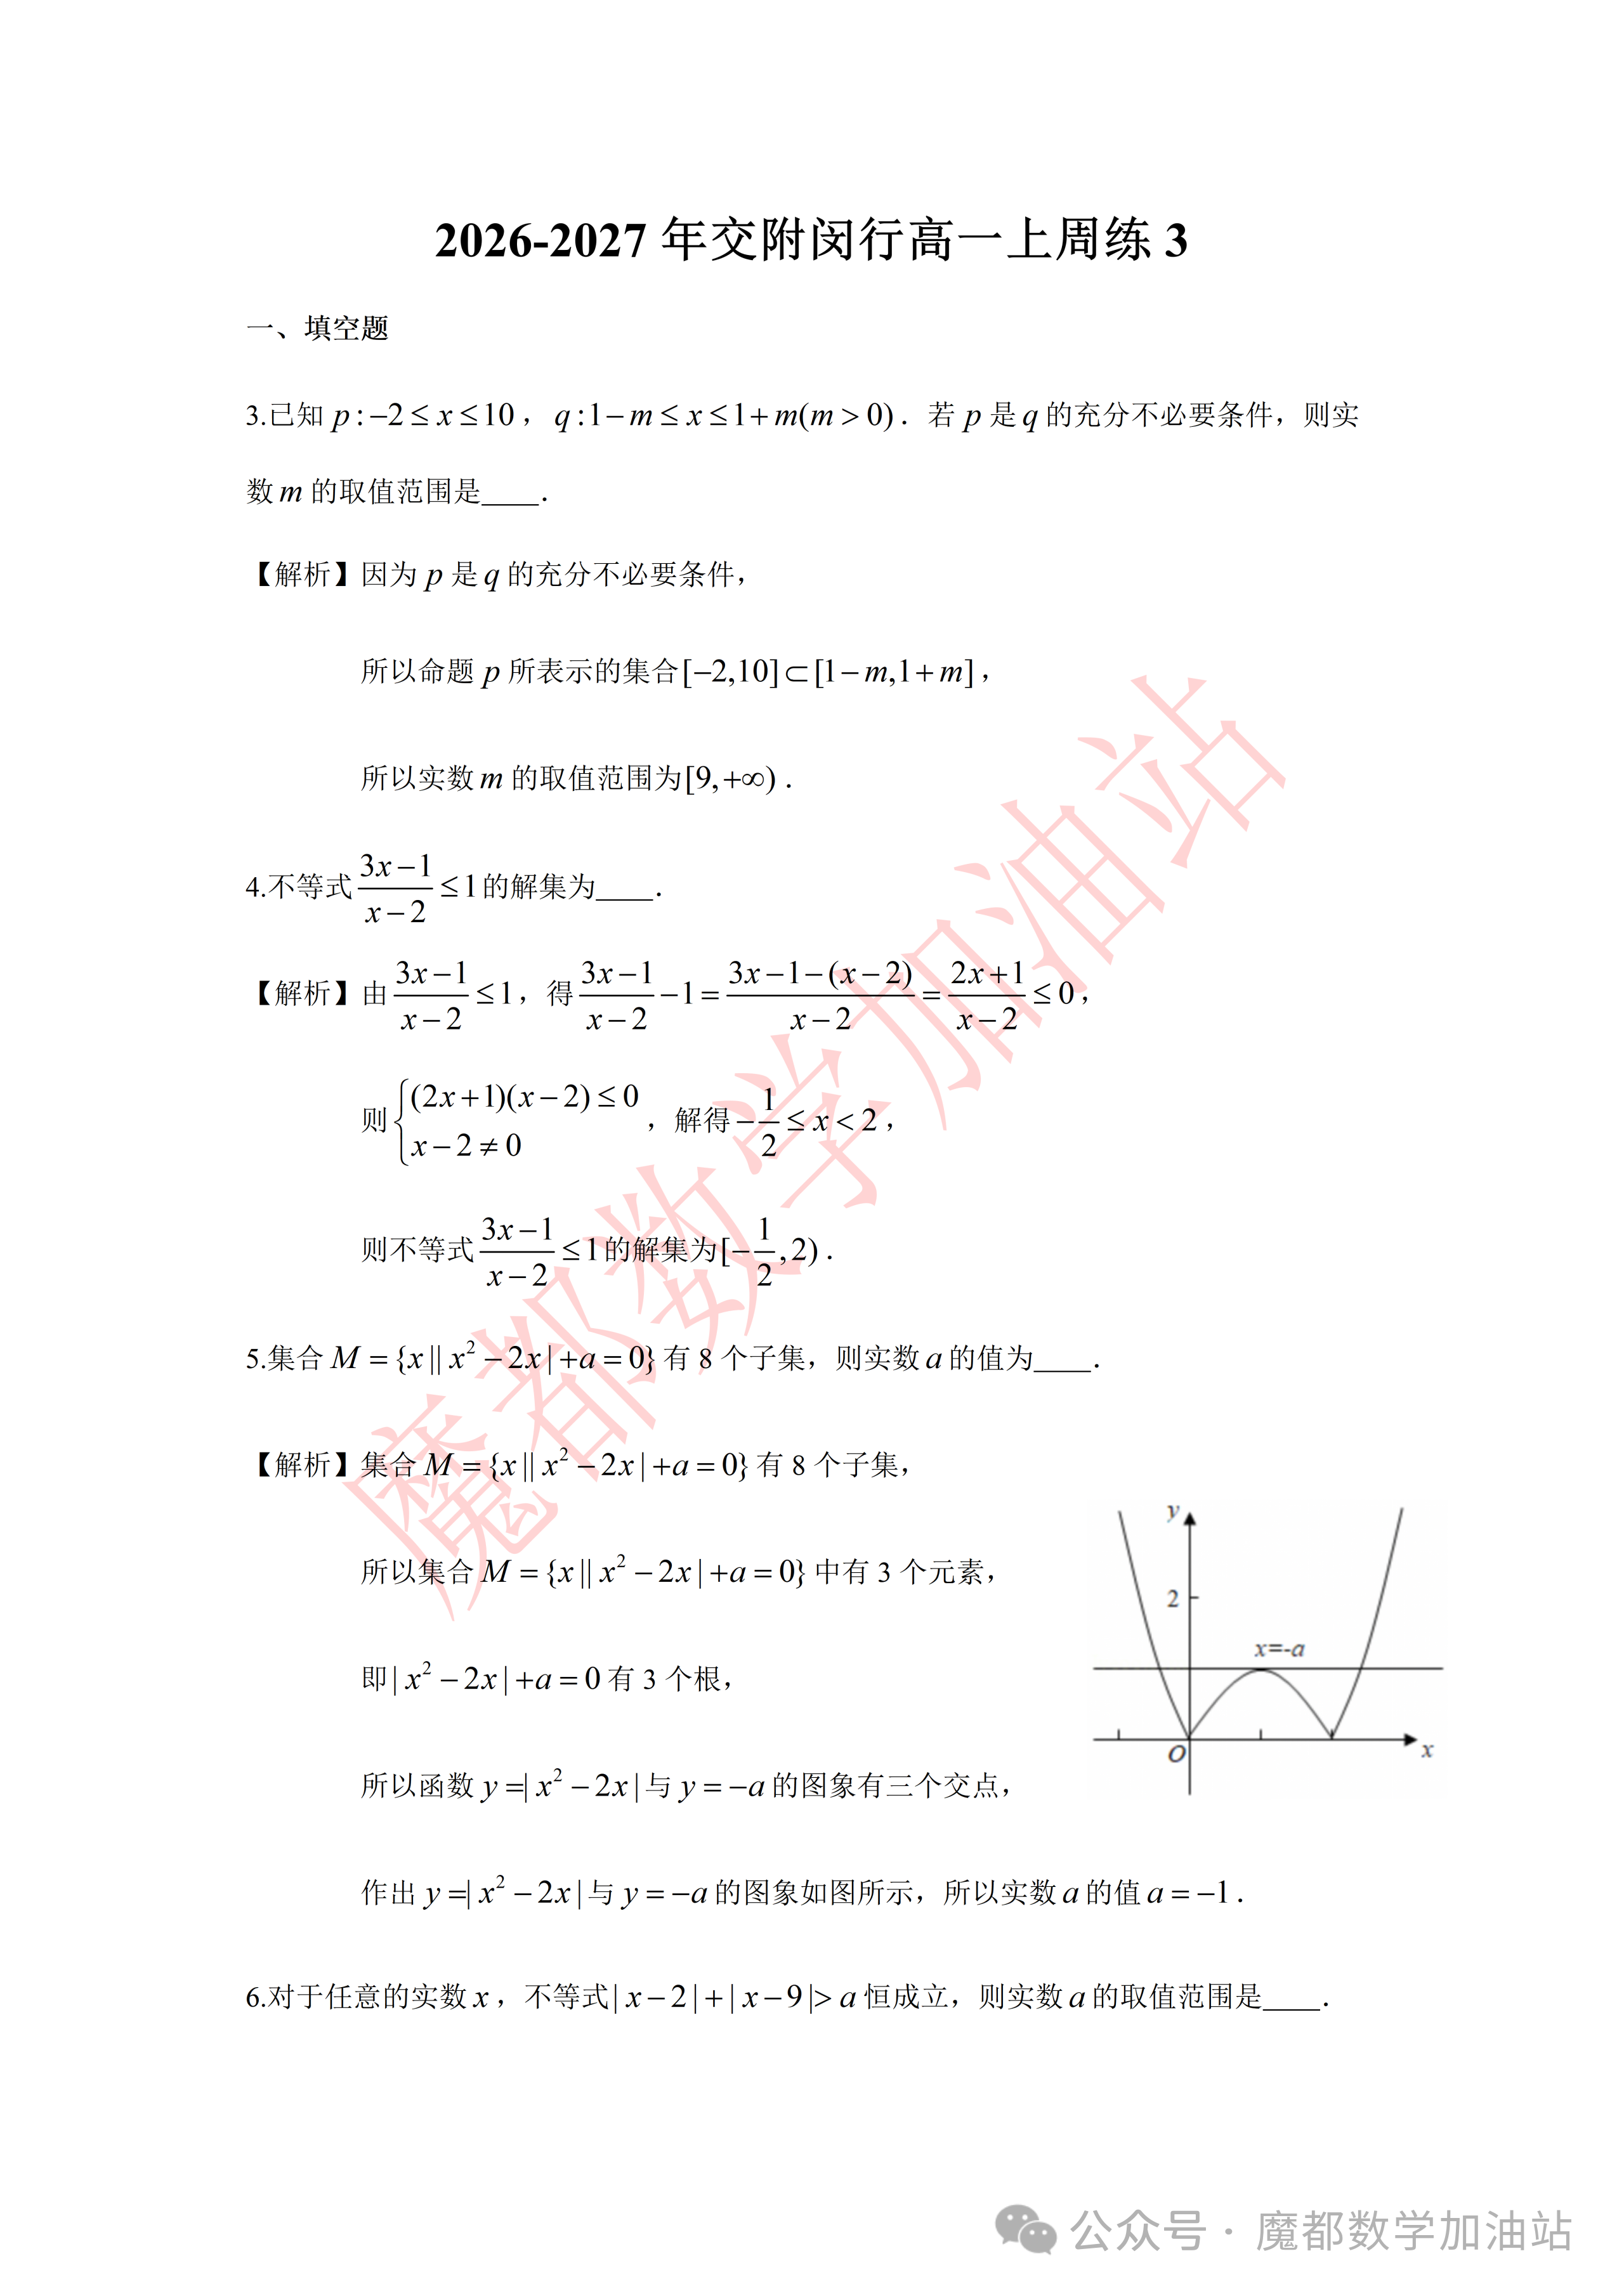
\includegraphics[width=0.14\textwidth,trim={1721bp 837bp 280bp 2297bp},clip]{../原图/高一43_交附闵行_周练3/01.png}
\end{center}

\solbegin
\step{集合 $M=\{x\mid |x^2-2x|+a=0\}$ 有 8 个子集，}
\step{所以集合 $M=\{x\mid |x^2-2x|+a=0\}$ 中有 3 个元素，}
\step{即 $|x^2-2x|+a=0$ 有 3 个根，}
\step{所以函数 $y=|x^2-2x|$ 与 $y=-a$ 的图象有三个交点，}
\step{作出 $y=|x^2-2x|$ 与 $y=-a$ 的图象如图所示，所以实数 $a$ 的值 $a=-1$.}
\solend

\fi

\item 对于任意的实数 $x$，不等式 $|x-2|+|x-9|>a$ 恒成立，则实数 $a$ 的取值范围是 \blankline[4.4em].

\ifanswer
\solbegin
\step{由绝对值的几何意义得 $|x-2|+|x-9|\geqslant7$，当且仅当 $2\leqslant x\leqslant9$ 时等号成立，}
\step{所以 $a<7$，}
\step{即 $a$ 的取值范围为 $(-\infty,7)$.}
\solend

\fi

\item 已知集合 $A=\{x\mid(a-1)x^2+3x-2=0\}$，$B=\{x\mid x^2-3x+2=0\}$，$A\subseteq B$，求实数 $a$ 的取值范围是 \blankline[4.4em].

\ifanswer
\solbegin
\step{由方程 $x^2-3x+2=0$，解得 $x=1$ 或 $x=2$，即 $B=\{1,2\}$，}
\step{因为 $A\subseteq B$，所以 $A=\varnothing$ 或 $A=\{1\}$ 或 $A=\{2\}$ 或 $A=\{1,2\}$，}
\step{当 $A=\varnothing$ 时，$a\neq1$，且 $\Delta=3^2-4(a-1)\times(-2)<0$，解得 $a<-\dfrac18$，}
\step{将 $x=1$ 代入方程 $(a-1)x^2+3x-2=0$，得 $a=0$，}
\step{此时 $A=\{x\mid-x^2+3x-2=0\}=\{1,2\}$，满足条件，}
\step{将 $x=2$ 代入方程 $(a-1)x^2+3x-2=0$，得到 $a=0$，上面已经验证满足条件，}
\step{综上所述，$a$ 的取值范围是 $\left(-\infty,-\dfrac18\right)\cup\{0\}$.}
\solend

\fi

\item 已知 $a$、$b$、$c$、$d$ 为常数，若不等式
$\dfrac{b}{x+a}+\dfrac{x+d}{x+c}<0$ 的解集为 $\left(-1,-\dfrac13\right)\cup\left(\dfrac12,1\right)$，
则不等式 $\dfrac{bx}{ax-1}+\dfrac{dx-1}{cx-1}<0$ 的解集为 \blankline[4.4em].

\ifanswer
\solbegin
\step{若 $x=0$，原不等式化为 $1<0$，不等式显然不成立，所以 $x\neq0$，}
\step{由 $\dfrac{bx}{ax-1}+\dfrac{dx-1}{cx-1}<0$，得 $\dfrac{b}{a-\dfrac1x}+\dfrac{d-\dfrac1x}{c-\dfrac1x}<0$，即 $\dfrac{b}{-\dfrac1x+a}+\dfrac{-\dfrac1x+d}{-\dfrac1x+c}<0$.}
\step{因为不等式 $\dfrac{b}{x+a}+\dfrac{x+d}{x+c}<0$ 的解集为 $\left(-1,-\dfrac13\right)\cup\left(\dfrac12,1\right)$，}
\step{所以 $-1<-\dfrac1x<-\dfrac13$ 或 $\dfrac12<-\dfrac1x<1$，解得 $1<x<3$ 或 $-2<x<-1$，}
\step{所以不等式 $\dfrac{bx}{ax-1}+\dfrac{dx-1}{cx-1}<0$ 的解集为 $(-2,-1)\cup(1,3)$.}
\solend

\fi

\item 正实数 $x$、$y$ 满足 $2x+3y-xy=0$，且存在这样的 $x$、$y$ 使不等式 $x+y<m+1$ 有解，则实数 $m$ 的取值范围是 \blankline[4.4em].

\ifanswer
\solbegin
\step{因为正实数 $x$、$y$ 满足 $2x+3y-xy=0$，则 $\dfrac2y+\dfrac3x=1$，$x>0$，$y>0$，}
\step{所以 $x+y=(x+y)\left(\dfrac3x+\dfrac2y\right)=3+\dfrac{2x}{y}+\dfrac{3y}{x}+2\geqslant2\sqrt{\dfrac{2x}{y}\times\dfrac{3y}{x}}+5=5+2\sqrt6$，}
\step{当且仅当 $\sqrt2x=\sqrt3y$ 时取等号，}
\step{存在这样的 $x$、$y$ 使不等式 $x+y<m+1$ 有解，则 $m+1>5+2\sqrt6$，}
\step{则 $m>4+2\sqrt6$，所以实数 $m$ 的取值范围是 $(4+2\sqrt6,+\infty)$.}
\solend

\fi

\item 若 $a$、$b$、$c\in\R$，$a^2+b^2+c^2=1$，则 $2ab+bc$ 的最大值为 \blankline[4.4em].

\ifanswer
\solbegin
\step{对于 $2ab+bc$，将 $b^2$ 拆分为 $\dfrac45b^2+\dfrac15b^2$，则 $a^2+\dfrac45b^2+c^2+\dfrac15b^2=1$，}
\step{$a^2+\dfrac45b^2\geqslant2\cdot a\cdot\dfrac2{\sqrt5}b=\dfrac4{\sqrt5}ab$，$c^2+\dfrac15b^2\geqslant2\cdot c\cdot\dfrac1{\sqrt5}b=\dfrac2{\sqrt5}bc$，}
\step{两式相加得 $1\geqslant\dfrac4{\sqrt5}ab+\dfrac2{\sqrt5}bc=\dfrac2{\sqrt5}(2ab+bc)$，故 $2ab+bc\leqslant\dfrac{\sqrt5}2$，}
\step{等号成立当且仅当 $a=\dfrac2{\sqrt5}b$，$c=\dfrac1{\sqrt5}b$，}
\step{代入 $a^2+b^2+c^2=1$，得 $\dfrac45b^2+b^2+\dfrac15b^2=2b^2=1$，即 $b=\dfrac{\sqrt2}2$，}
\step{此时 $a=\dfrac{\sqrt{10}}5$，$c=\dfrac{\sqrt{10}}{10}$，故 $2ab+bc$ 的最大值为 $\dfrac{\sqrt5}2$.}
\solend

\fi

\item 已知实数 $a$、$b$ 满足 $-3<a+2b<2$，$-1<2a-b<4$，则 $a+b$ 的取值范围为 \blankline[4.4em].

\ifanswer
\solbegin
\step{设 $a+b=m(a+2b)+n(2a-b)=(m+2n)a+(2m-n)b$，}
\step{所以 $\begin{cases}m+2n=1\\2m-n=1\end{cases}$，解得 $n=\dfrac15$，$m=\dfrac35$，所以 $a+b=\dfrac35(a+2b)+\dfrac15(2a-b)$，}
\step{因为 $-3<a+2b<2$，$-1<2a-b<4$，}
\step{所以 $-\dfrac95<\dfrac35(a+2b)<\dfrac65$，$-\dfrac15<\dfrac15(2a-b)<\dfrac45$，}
\step{相加得 $-2<\dfrac35(a+2b)+\dfrac15(2a-b)<2$，即 $-2<a+b<2$，}
\step{故 $a+b$ 的取值范围为 $(-2,2)$.}
\solend

\fi

% 注：原卷题干与解析均印作 \sqrt{2xyz}，但按其自身答案 8 与取等值（$y=\dfrac12$，
% $x=\dfrac{\sqrt3}4$，$z=\dfrac{\sqrt6}4$）代入只与 $\sqrt{2x^2y^2z^2}=\sqrt2\,xyz$ 相符，
% $\sqrt{2xyz}$ 与答案 8 不自洽，原卷如此，照录未改。
\item 已知正数 $x$、$y$、$z$ 满足 $2x^2+y^2+z^2=1$，则 $\dfrac{y+1}{\sqrt{2xyz}}$ 的最小值为 \blankline[4.4em].

\ifanswer
\solbegin
\step{由条件得 $2x^2+z^2=1-y^2=(1-y)(1+y)$，则 $1+y=\dfrac{2x^2+z^2}{1-y}$，}
\step{结合 $x$、$y$、$z>0$ 得原式 $=\dfrac{2x^2+z^2}{\sqrt{2xyz}(1-y)}\geqslant\dfrac{2\sqrt2xz}{\sqrt{2xyz}(1-y)}=\dfrac2{y(1-y)}$，}
\step{又 $y(1-y)\leqslant\left(\dfrac{y+1-y}2\right)^2=\dfrac14$，所以 $\dfrac2{y(1-y)}\geqslant\dfrac2{\frac14}=8$，}
\step{当且仅当 $\sqrt2x=z$，且 $y=1-y$，即 $y=\dfrac12$，$x=\dfrac{\sqrt3}4$，$z=\dfrac{\sqrt6}4$ 时取等号，}
\step{故 $\dfrac{y+1}{\sqrt{2xyz}}$ 最小值为 $8$.}
\solend

\fi

\end{enumerate}

\bigsec{二、选择题}

\begin{enumerate}
\setcounter{enumi}{12}

\item 已知关于 $x$ 的方程 $(1-k)x^2-2x-1=0$ 有实数根，则 $k$ 的取值范围是\mbox{（\quad）}

\keepwithprev
A. $k\leqslant2$ 且 $k\neq1$\qquad B. $k\leqslant2$\qquad
C. $k<2$ 且 $k\neq1$\qquad D. $k<2$

\ans{$A$}

\ifanswer
\solbegin
\step{由题意得 $\begin{cases}1-k\neq0\\\Delta=4+4(1-k)\geqslant0\end{cases}$，解不等式得 $\begin{cases}1\neq k\\2-k>0\end{cases}$，所以 $k\leqslant2$ 且 $k\neq1$，}
\step{故选 $A$.}
\solend

\fi

\item 不等式 $2|x+2|+|x-1|\geqslant5$ 成立的一个必要不充分条件是\mbox{（\quad）}

\keepwithprev
A. $x\leqslant-1$ 或 $x\geqslant0$\qquad B. $x\geqslant0$

C. $x\leqslant-\dfrac83$ 或 $x\geqslant0$\qquad D. $x\geqslant1$

\ans{$A$}

\ifanswer
\solbegin
\step{当 $x<-2$ 时，原不等式可化为 $-2x-4-x+1\geqslant5$，解得 $x\leqslant-\dfrac83$，}
\step{当 $-2\leqslant x<1$ 时，原不等式可化为 $2x+4-x+1\geqslant5$，解得 $0\leqslant x<1$，}
\step{当 $x\geqslant1$ 时，原不等式可化为 $2x+4+x-1\geqslant5$，解得 $x\geqslant\dfrac23$，得 $x\geqslant1$，}
\step{综上所述，不等式 $2|x+2|+|x-1|\geqslant5$ 成立的充要条件是 $x\leqslant-\dfrac83$ 或 $x\geqslant0$，}
\step{设 $A=\{x\mid x\leqslant-\dfrac83\text{ 或 }x\geqslant0\}$，}
\step{则不等式 $2|x+2|+|x-1|\geqslant5$ 成立的必要不充分条件，}
\step{其对应的集合 $B$ 满足 $A\subsetneq B$，对照各个选项，$A$ 项符合题意. 故选 $A$.}
\solend

\fi

\item 已知实数 $a>0$，$b>0$，$\dfrac1{a+1}+\dfrac1{b+1}=1$，则 $2a+3b$ 的最小值为\mbox{（\quad）}

\keepwithprev
A. $2\sqrt6$\qquad B. $3+2\sqrt6$\qquad
C. $5+2\sqrt6$\qquad D. $3+2\sqrt2$

\ans{$A$}

\ifanswer
\solbegin
\step{因为 $a>0$，$b>0$，$\dfrac1{a+1}+\dfrac1{b+1}=1$，}
\step{所以 $2a+3b=2(a+1)+3(b+1)-5=[2(a+1)+3(b+1)]\cdot\left(\dfrac1{a+1}+\dfrac1{b+1}\right)-5$}
\step{$=\left[2+3+\dfrac{3(b+1)}{a+1}+\dfrac{2(a+1)}{b+1}\right]-5\geqslant5+2\sqrt{\dfrac{3(b+1)}{a+1}\times\dfrac{2(a+1)}{b+1}}-5=2\sqrt6$，}
\step{当且仅当 $\dfrac{3(b+1)}{a+1}=\dfrac{2(a+1)}{b+1}$，即 $a=\dfrac{\sqrt6}2$，$b=\dfrac{\sqrt6}3$ 时取等号. 故选 $A$.}
\solend

\fi

\item 已知集合 $U=\{n\mid1\leqslant n\leqslant2027,\ n\in\N\}$，集合 $M\subseteq U$，若对于 $M$ 中任意两个不同的元素 $x$ 和 $y$，都有 $|x-y|>2$，则 $M$ 中元素个数的最大值是\mbox{（\quad）}

\keepwithprev
A. $676$\qquad B. $675$\qquad C. $672$\qquad D. $671$

\ans{$A$}

\ifanswer
\solbegin
\step{对于 $M$ 中的任意两个不同的元素 $x$、$y$，都有 $|x-y|>2$，}
\step{不妨设 $x>y$，都有 $x-y\geqslant3$，}
\step{要想 $M$ 所含元素个数最大，则要 $x-y$ 尽可能小，故需使得 $x-y$ 的最小值为 3，}
\step{将 $1\sim2027$ 这 2027 个元素按如下分组：}
\step{$\{1,2,3\}$，$\{4,5,6\}$，$\cdots$，$\{2023,2024,2025\}$，$\{2026,2027\}$，}
\step{故应在前 675 组中按周期 3 每组取一个元素，且第一组中不能取 3，}
\step{第一组中取 1 时，得 $M=\{1,4,7,\cdots,2023,2026\}$，}
\step{或 $M=\{1,4,7,\cdots,2023,2027\}$ 这样的集合，}
\step{第一组取 2 时，得 $M=\{2,5,8,\cdots,2024,2027\}$，}
\step{其中任意两元素差值 $x-y$（$x>y$）都大于 2，满足题意，}
\step{故 $M$ 所含元素个数的最大值为 $\dfrac{2025}{3}+1=676$. 故选 $A$.}
\solend

\fi

\end{enumerate}

\bigsec{三、解答题}

\begin{enumerate}
\setcounter{enumi}{16}

\item 已知 $a\in\R$，集合 $A=\left\{x\middle|\dfrac{2-x}{x+1}\leqslant0\right\}$，$B=\{x\mid x^2+(3-a)x-3a<0\}$.

\begin{enumerate}[label=(\arabic*)]
\item 当 $a=\dfrac13$ 时，求 $A$ 和 $B$；
\item 已知 $A\cup B=A$，求实数 $a$ 的取值范围.
\end{enumerate}

\ifanswer
\solbegin
\stepm{(1)}{由 $\dfrac{2-x}{x+1}\leqslant0$，得 $\begin{cases}(2-x)(x+1)\leqslant0\\x\neq-1\end{cases}$，解得 $x<-1$ 或 $x\geqslant2$，}
\step{则 $A=\{x\mid x<-1\text{ 或 }x\geqslant2\}$；}
\step{$B=\{x\mid x^2+(3-a)x-3a<0\}=\{x\mid(x+3)(x-a)<0\}$，}
% 注：原卷此行印作 $(x+2)\left(x-\dfrac13\right)$，按前一行 $B=\{x\mid(x+3)(x-a)<0\}$ 应为
% $(x+3)\left(x-\dfrac13\right)$，原卷如此，照录未改。
\step{当 $a=\dfrac13$ 时，$B=\left\{x\middle|(x+2)\left(x-\dfrac13\right)<0\right\}$，}
\step{解得 $B=\left\{x\middle|-3<x<\dfrac13\right\}$.}
\stepm{(2)}{由 $A\cup B=A$，得 $B\subseteq A$，}
\step{①当 $B=\varnothing$ 时，得 $a=-3$，符合题意；}
\step{②当 $B\neq\varnothing$ 时，若 $a>-3$，则 $B=\{x\mid-3<x<a\}$，}
\step{由 $B\subseteq A$，得 $a\leqslant-1$，此时 $-3<a\leqslant-1$；}
\step{若 $a<-3$，则 $B=\{x\mid a<x<-3\}$，此时 $B\subseteq A$ 恒成立，}
\step{故 $a<-3$ 符合题意；}
\step{综上所述，实数 $a$ 的取值范围为 $a\leqslant-1$.}
\solend

\fi

\ansspace[6]

\item 甲乙两地的高速公路全长 166 千米，汽车从甲地进入该高速公路后匀速行驶到乙地，车速 $v\in[70,120]$（千米/时）. 已知汽车每小时的运输成本（以元为单位）由可变部分和固定部分组成：可变部分为 $0.02v^2$，固定部分为 220 元.

\begin{enumerate}[label=(\arabic*)]
\item 若每小时的运输成本不高于 420 元，汽车的速度应该控制在什么范围？
\item 汽车应以多大速度行驶才能使全程运输成本最小？最小运输成本约为多少元？（结果保留整数）
\end{enumerate}

\ifanswer
\solbegin
\stepm{(1)}{已知汽车每小时的运输成本（以元为单位）由可变部分和固定部分组成：}
\step{可变部分为 $0.02v^2$，固定部分为 220 元，}
\step{则汽车每小时的运输成本为 $0.02v^2+220$（元），}
\step{若每小时的运输成本不高于 420 元，}
\step{则 $0.02v^2+220\leqslant420$，解得 $v^2\leqslant10000$，}
\step{得 $70\leqslant v\leqslant100$，即 $v\in[70,100]$（千米/时），}
\step{则此时汽车的速度 $v$ 应该控制在 $[70,100]$（千米/时）；}
\stepm{(2)}{因为汽车从甲地进入该高速公路后匀速行驶到乙地，}
\step{车速 $v\in[70,120]$（千米/时），所以汽车的行驶时间为 $\dfrac{166}{v}$（小时），}
\step{所以全程运输成本 $y=\dfrac{166}{v}(0.02v^2+220)=3.32v+\dfrac{36520}{v}$，}
% 注：原卷此行印作 $v\in[70,100]$，与题干的 $v\in[70,120]$ 不自洽（若 $v\in[70,100]$，
% 最小值应在 $v=100$ 处取得，与下文 $v=10\sqrt{110}\approx105$ 矛盾），原卷如此，照录未改。
\step{$v\in[70,100]$，}
\step{由基本不等式得 $y=3.32v+\dfrac{36520}{v}\geqslant2\sqrt{3.32v\times\dfrac{36520}{v}}\approx696$，}
\step{当且仅当 $3.32v=\dfrac{36520}{v}$，即 $v=10\sqrt{110}\approx105$ 时取等号，}
\step{汽车应以 105（千米/时）行驶才能使全程运输成本最小，}
\step{最小运输成本约为 696 元.}
\solend

\fi

\ansspace[8]

\item
\begin{enumerate}[label=(\arabic*)]
\item 已知 $a$、$b$、$c$ 为实数，求证：$|a-b|\leqslant|a-c|+|b-c|$，并说明等号成立的条件；
\item 设 $x\in\R$，求方程 $|3x-8|=|5-x|+|2x-3|$ 的解集.
\end{enumerate}

\ifanswer
% 注：原卷第 19 题未印【解析】，仅印一行【答案】"（1）(a-c)(b-c)≤0；
% （2）(-∞,3/2]∪[5,+∞)"。(1) 的两行推导为本稿所补，(2) 照录原卷答案。
% 又题干作"方程"，而所给答案 (-∞,3/2]∪[5,+∞) 实为不等式 |3x-8|≤|5-x|+|2x-3| 的解集，
% 与"方程"不合，原卷如此，照录未改。
\solbegin
\stepm{(1)}{由三角不等式 $|a-b|=|(a-c)-(b-c)|\leqslant|a-c|+|b-c|$，}
\step{当且仅当 $(a-c)(b-c)\leqslant0$ 时等号成立.}
\stepm{(2)}{$\left(-\infty,\dfrac32\right]\cup[5,+\infty)$.}
\solend

\fi

\ansspace[6]

\item 已知正实数 $a$、$b$ 满足 $a+b=1$，求 $\dfrac1a+\dfrac1b$ 的最小值. 其中一种解法是：

\[
\begin{aligned}
\dfrac1a+\dfrac1b
&=\left(\dfrac1a+\dfrac1b\right)(a+b)\\
&=1+\dfrac ba+\dfrac ab+1\\
&\geqslant2+2\sqrt{\dfrac ba\times\dfrac ab}=2+2=4.
\end{aligned}
\]
当且仅当 $\dfrac ba=\dfrac ab$ 且 $a+b=1$ 时即 $a=b=\dfrac12$ 时取等号.
学习上述解法并解决下列问题：

\begin{enumerate}[label=(\arabic*)]
\item 若正实数 $x$、$y$ 满足 $x+y=xy$，求 $2x+y$ 的最小值；
\item 若实数 $a$、$b$、$x$、$y$ 满足 $\dfrac{x^2}{a^2}+\dfrac{y^2}{b^2}=1$，求证：$a^2+b^2\geqslant(x+y)^2$；
\item 求代数式 $M=\sqrt{m-1}+\sqrt{3-m}$ 的最大值，并求出使得 $M$ 最大的 $m$ 的值.
\end{enumerate}

\ifanswer
\solbegin
\stepm{(1)}{因为正实数 $x$、$y$ 满足 $x+y=xy$，$\dfrac{x+y}{xy}=1\Rightarrow\dfrac1y+\dfrac1x=1$，}
\step{所以 $(2x+y)\times1=(2x+y)\left(\dfrac1y+\dfrac1x\right)=3+\dfrac{2x}{y}+\dfrac yx\geqslant3+2\sqrt{\dfrac{2x}{y}\cdot\dfrac yx}=3+2\sqrt2$，}
\step{当且仅当 $\dfrac{2x}{y}=\dfrac yx$ 且 $\dfrac1y+\dfrac1x=1$ 时取等号，}
\step{解得 $x=\dfrac{2+\sqrt2}2$，$y=\sqrt2x=\sqrt2\times\dfrac{2+\sqrt2}2=1+\sqrt2$，}
\step{所以 $2x+y$ 的最小值为 $3+2\sqrt2$；}
\stepm{(2)}{因为 $\dfrac{x^2}{a^2}+\dfrac{y^2}{b^2}=1$，}
\step{所以 $a^2+b^2=(a^2+b^2)\left(\dfrac{x^2}{a^2}+\dfrac{y^2}{b^2}\right)=x^2+y^2+\dfrac{b^2x^2}{a^2}+\dfrac{a^2y^2}{b^2}$，}
\step{因为 $\dfrac{b^2x^2}{a^2}+\dfrac{a^2y^2}{b^2}\geqslant2\sqrt{\dfrac{b^2x^2}{a^2}\times\dfrac{a^2y^2}{b^2}}=2\sqrt{x^2y^2}=2|xy|$，}
\step{当且仅当 $\dfrac{b^2x^2}{a^2}=\dfrac{a^2y^2}{b^2}$ 时取等号，}
\step{所以 $x^2+y^2+\dfrac{b^2x^2}{a^2}+\dfrac{a^2y^2}{b^2}\geqslant x^2+y^2+2|xy|\geqslant x^2+y^2+2xy=(x+y)^2$，}
\step{所以 $a^2+b^2\geqslant(x+y)^2$；}
\stepm{(3)}{因为 $M=\sqrt{m-1}+\sqrt{3-m}$，所以 $\begin{cases}m-1\geqslant0\\3-m\geqslant0\end{cases}$，解得 $1\leqslant m\leqslant3$，}
\step{所以 $M^2=(\sqrt{m-1}+\sqrt{3-m})^2=2+2\sqrt{(3-m)(m-1)}$，}
\step{由基本不等式得 $(3-m)(m-1)\leqslant\left(\dfrac{(3-m)+(m-1)}2\right)^2=1$，}
\step{当且仅当 $3-m=m-1$ 时取等号，解得 $m=2$，}
\step{所以 $M^2=2+2\sqrt{(3-m)(m-1)}\leqslant2+2\sqrt1=4$，}
\step{因为 $M>0$，所以 $M\leqslant2$，所以 $M$ 最大值为 2，此时 $m$ 的值为 2.}
\solend

\fi

\ansspace[8]

\item 若有限个正整数组成的集合 $A$ 中至少有两个元素，且对于任意的 $x,y\in A$（$x>y$），都有 $\dfrac{y^2}{x-y}\in A$，则称 $A$ 为“L-集合”.

\begin{enumerate}[label=(\arabic*)]
\item 判断 $\{1,2,4\}$ 是否为“L-集合”，说明理由；
\item 若双元素集 $M$ 为“L-集合”，且 $4\in M$，求所有满足条件的集合 $M$；
\item 求所有满足条件的“L-集合”.
\end{enumerate}

\ifanswer
\solbegin
\stepm{(1)}{若至少由两个元素构成的有限集合 $A\subseteq\N^*$，}
% 注：原卷下一行"都有"后未印分数 \dfrac{y^2}{x-y}，径作"都有 A"，原卷如此，照录未改。
\step{且对于任意的 $x$、$y\in A$（$x>y$），都有 $A$，则称 $A$ 为“L-集合”，}
\step{$\{1,2,4\}$ 不为“L-集合”，理由如下：}
\step{因为 $\dfrac{1^2}{4-1}=\dfrac13\notin\{1,2,4\}$，所以 $\{1,2,4\}$ 不是“L-集合”.}
\stepm{(2)}{设 $M=\{4,m\}$（$m\in\N^*$，$m\neq4$），}
\step{若 $m<4$，则 $\dfrac{m^2}{4-m}=m$ 或 $\dfrac{m^2}{4-m}=4$，}
\step{由 $\dfrac{m^2}{4-m}=m$，解得 $m=2$，$m=0$（舍去），此时 $M=\{2,4\}$；}
\step{由 $\dfrac{m^2}{4-m}=4$ 化为 $m^2+4m-16=0$，而 $\Delta=4^2+4\times16=80$，}
\step{故方程无正整数解.}
\step{若 $m>4$，则 $\dfrac{4^2}{m-4}=4$ 或 $\dfrac{4^2}{m-4}=m$，}
\step{由 $\dfrac{4^2}{m-4}=4$，解得 $m=8$，此时 $M=\{4,8\}$；}
\step{由 $\dfrac{4^2}{m-4}=m$ 化为 $m^2-4m-16=0$，而 $\Delta=4^2+4\times16=80$，}
\step{故方程无正整数解.}
\step{综上，双元素集 $M$ 为“L-集合”，且 $4\in M$，}
\step{则所有满足条件的集合 $M$ 为 $\{4,8\}$，$\{2,4\}$.}
\stepm{(3)}{若“L-集合”为双元素集，}
\step{不妨设 $M=\{k,m\}$（$k,m\in\N^*$，$m>k$），则 $\dfrac{k^2}{m-k}=k$ 或 $\dfrac{k^2}{m-k}=m$，}
\step{由 $\dfrac{k^2}{m-k}=k$，则 $2k^2=mk$，而 $m>k$，故 $m=2k$，此时 $M=\{k,2k\}$；}
\step{由 $\dfrac{k^2}{m-k}=m$，则 $m^2-mk-k^2=0$，而 $\Delta=5k^2$，显然不存在正整数解；}
\step{所以，“L-集合”为 $\{k,2k\}$，其中 $k\in\N^*$.}
\step{若“L-集合”含有两个以上的元素，}
\step{设最小的元素为 $b$，最大的元素为 $a$，第二大的元素为 $n$，}
\step{则 $\dfrac{b^2}{a-b}$，$\dfrac{n^2}{a-n}$ 是“L-集合”中的元素，}
% 注：原卷下一行未印"由于'L-集合'中的元素均为正整数"一语，径作"若 \dfrac{b^2}{a-b}\geqslant b"，
% 原卷如此，照录未改。
\step{若 $\dfrac{b^2}{a-b}\geqslant b$，解得 $a\leqslant2b$，}
\step{若 $\dfrac{n^2}{a-n}\leqslant n$，则 $a\geqslant2n>2b$，矛盾，}
\step{若 $\dfrac{n^2}{a-n}=a$，该方程的解为 $n=\dfrac{\sqrt5-1}2a$，则 $n$、$a$ 不可能同时为整数，}
\step{无解.}
\step{所以所有满足条件的“L-集合”为 $\{k,2k\}$，其中 $k\in\N^*$.}
\solend

\fi

\ansspace*[10]

\end{enumerate}

\end{document}
"
% 紧凑版：xelatex "\def\iscompact{1}% 高一43_交附闵行_周练3.tex
%   —— 高一上数学“2026-2027 年交附闵行高一上周练3”（试卷版/答案版）
% 试卷版：xelatex 高一43_交附闵行_周练3.tex
% 答案版：xelatex "\def\isanswer{1}% 高一43_交附闵行_周练3.tex
%   —— 高一上数学“2026-2027 年交附闵行高一上周练3”（试卷版/答案版）
% 试卷版：xelatex 高一43_交附闵行_周练3.tex
% 答案版：xelatex "\def\isanswer{1}% 高一43_交附闵行_周练3.tex
%   —— 高一上数学“2026-2027 年交附闵行高一上周练3”（试卷版/答案版）
% 试卷版：xelatex 高一43_交附闵行_周练3.tex
% 答案版：xelatex "\def\isanswer{1}\input{高一43_交附闵行_周练3.tex}"
% 紧凑版：xelatex "\def\iscompact{1}\input{高一43_交附闵行_周练3.tex}"
%
% 原始材料是微信公众号图文（公众号“魔都数学加油站”，作者破晓，2026-10-01 21:37，
% 原文标题“27学年高一43——2026-2027年上海市交附闵行高一上周练3”，
% https://mp.weixin.qq.com/s/-rgkOD9jJVpug6s0uSbwmQ）。正文为 12 张 PNG 页；
% 第 01、05、09、12 页 2560×3620，其余第 02—04、06—08、10—11 页 4762×6735。
% 原文本身是讲评版，题目下方印有解析/答案；题目与讲解照原卷转录，保留原卷错误。
%
% 卷首标题：原卷印作“2026-2027 年交附闵行高一上周练3”，公众号标题中的“上海市”
% 三字不在卷面标题中，本稿依卷面录入；年份区间按全稿惯例排 en dash。
%
% 与原卷的排版差异：
%   ① 原文从第 3 题开始（第 1、2 题未在这篇推文中发布），本稿保留原题号 3—21；
%   ② 原卷本就印有“一、填空题”“二、选择题”“三、解答题”，本稿照原卷分节，
%      改排为全稿统一的大节标题；
%   ③ 原卷未印副标题，本稿按“知识模块”口径补出“集合与常用逻辑用语、不等式”；
%   ④ 原卷填空横线依全稿惯例排为 \blankline[4.4em]；选择题答案只在答案版以 \ans{} 显示，
%      解答区以 \ifanswer 分离；解答题按原卷留出标准作答空间；
%   ⑤ 第 5 题图取自原卷第 1 页截图并裁入本稿，不另建图档；公众号水印不录入。
%      原卷图页分页不保留，正文依本稿版心重新分页。
%
% 原卷存疑/错误（均照录，未改）：
%   ① 第 9 题原卷题干即作"正实数 x、y"，与解析 x>0、y>0 相容，并无矛盾（初稿曾误记
%      题干只称"实数"并据此指原卷不自洽，2026-10-05 回原图核对订正）。
%   ② 第 11 题解析"相加得"一行原卷印作 -2<3/5(a+2b)+1/5(2a-b)<2，第一项系数 3/5
%      原卷不缺（初稿漏抄致该行按字面不成立，2026-10-05 已按原卷补回）。
%   ③ 第 13 题答案印 A，解析以“1-k≠0”排除 k=1；但 k=1 时原方程为 -2x-1=0，
%      仍有实数根，按题意应选 B。本稿保留原卷答案 A 及其解析，不代为订正。
%
\documentclass[a4paper,11pt]{article}
\usepackage{common}
\usepackage{graphicx}

\begin{document}

\examtitlest[3]{2026--2027 年交附闵行高一上周练 3}{集合与常用逻辑用语、不等式}

\bigsec{一、填空题}

\begin{enumerate}
\setcounter{enumi}{2}

\item 已知 $p\colon -2\leqslant x\leqslant10$，$q\colon 1-m\leqslant x\leqslant1+m$（$m>0$）. 若 $p$ 是 $q$ 的充分不必要条件，则实数 $m$ 的取值范围是 \blankline[4.4em].

\ifanswer
\solbegin
\step{因为 $p$ 是 $q$ 的充分不必要条件，}
\step{所以命题 $p$ 所表示的集合 $[-2,10]\subset[1-m,1+m]$，}
\step{所以实数 $m$ 的取值范围为 $[9,+\infty)$.}
\solend

\fi

\item 不等式 $\dfrac{3x-1}{x-2}\leqslant1$ 的解集为 \blankline[4.4em].

\ifanswer
\solbegin
\step{由 $\dfrac{3x-1}{x-2}-1=\dfrac{3x-1-(x-2)}{x-2}=\dfrac{2x+1}{x-2}\leqslant0$，}
\step{则 $\begin{cases}(2x+1)(x-2)\leqslant0\\x-2\neq0\end{cases}$，解得 $-\dfrac12\leqslant x<2$，}
\step{则不等式 $\dfrac{3x-1}{x-2}\leqslant1$ 的解集为 $\left[-\dfrac12,2\right)$.}
\solend

\fi

\item 集合 $M=\{x\mid |x^2-2x|+a=0\}$ 有 8 个子集，则实数 $a$ 的值为 \blankline[4.4em].

\ifanswer
\begin{center}
% 图取自原卷第 1 页；用原图裁切，未重绘。
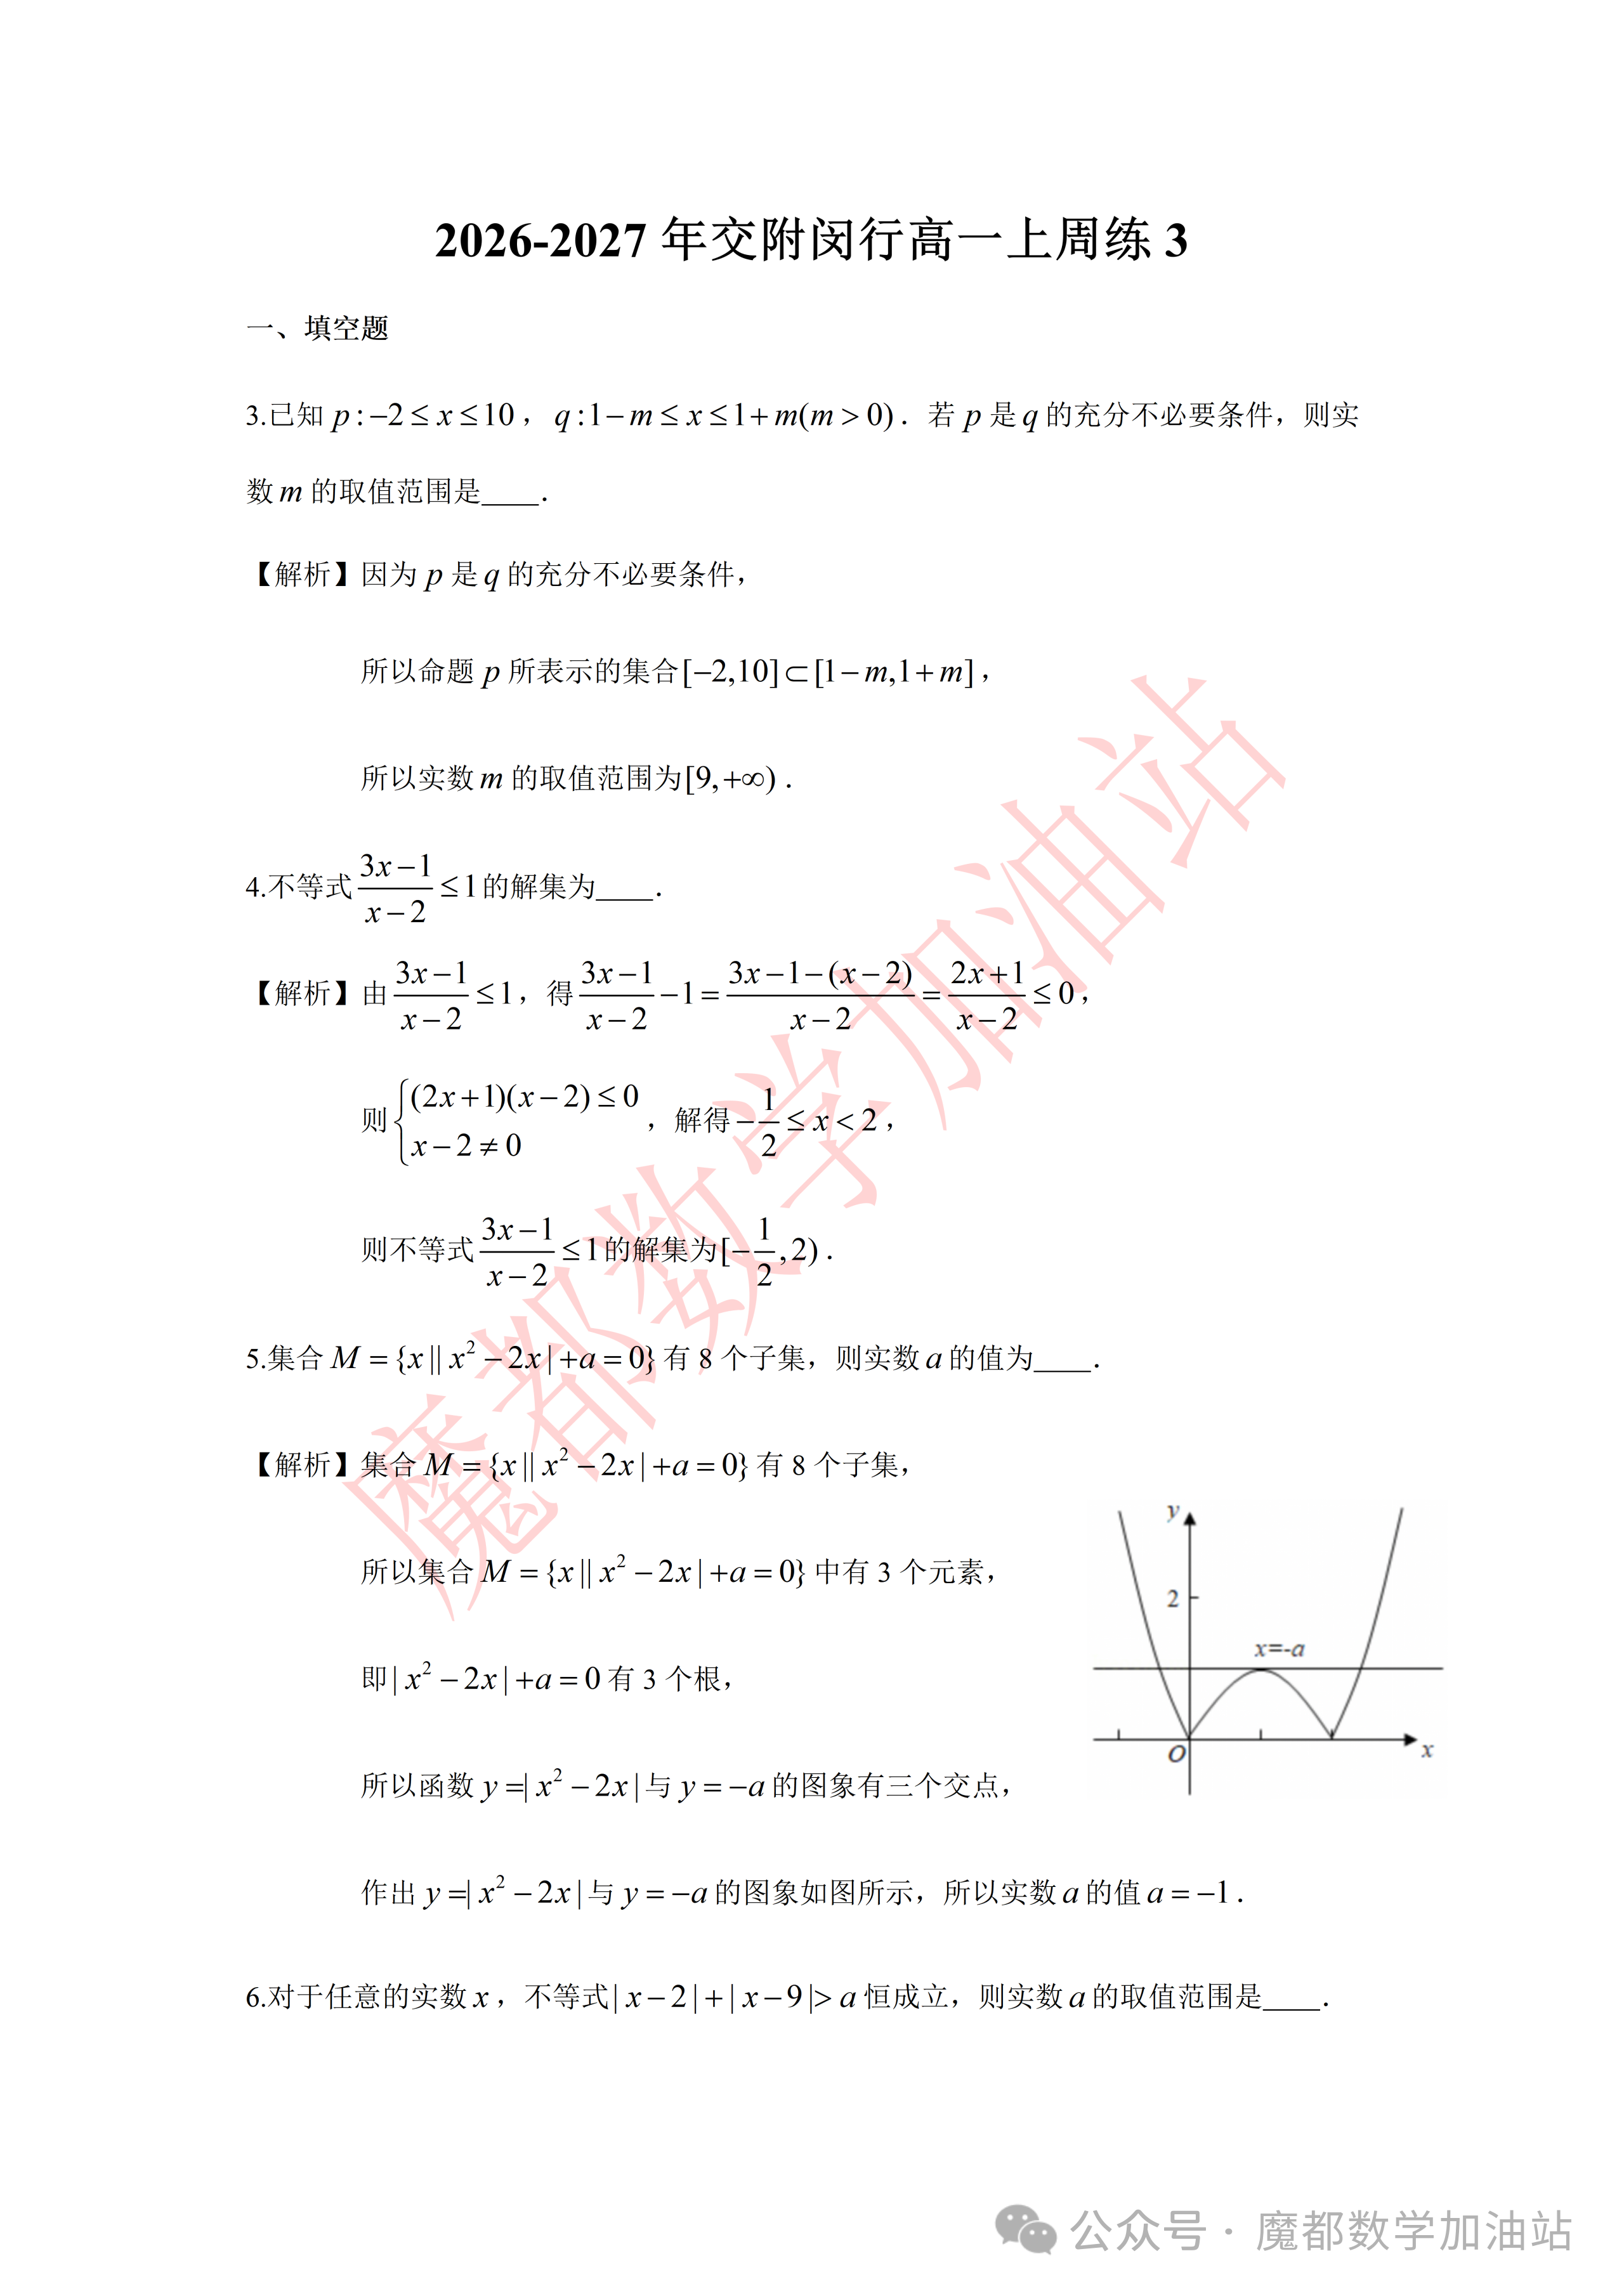
\includegraphics[width=0.14\textwidth,trim={1721bp 837bp 280bp 2297bp},clip]{../原图/高一43_交附闵行_周练3/01.png}
\end{center}

\solbegin
\step{集合 $M=\{x\mid |x^2-2x|+a=0\}$ 有 8 个子集，}
\step{所以集合 $M=\{x\mid |x^2-2x|+a=0\}$ 中有 3 个元素，}
\step{即 $|x^2-2x|+a=0$ 有 3 个根，}
\step{所以函数 $y=|x^2-2x|$ 与 $y=-a$ 的图象有三个交点，}
\step{作出 $y=|x^2-2x|$ 与 $y=-a$ 的图象如图所示，所以实数 $a$ 的值 $a=-1$.}
\solend

\fi

\item 对于任意的实数 $x$，不等式 $|x-2|+|x-9|>a$ 恒成立，则实数 $a$ 的取值范围是 \blankline[4.4em].

\ifanswer
\solbegin
\step{由绝对值的几何意义得 $|x-2|+|x-9|\geqslant7$，当且仅当 $2\leqslant x\leqslant9$ 时等号成立，}
\step{所以 $a<7$，}
\step{即 $a$ 的取值范围为 $(-\infty,7)$.}
\solend

\fi

\item 已知集合 $A=\{x\mid(a-1)x^2+3x-2=0\}$，$B=\{x\mid x^2-3x+2=0\}$，$A\subseteq B$，求实数 $a$ 的取值范围是 \blankline[4.4em].

\ifanswer
\solbegin
\step{由方程 $x^2-3x+2=0$，解得 $x=1$ 或 $x=2$，即 $B=\{1,2\}$，}
\step{因为 $A\subseteq B$，所以 $A=\varnothing$ 或 $A=\{1\}$ 或 $A=\{2\}$ 或 $A=\{1,2\}$，}
\step{当 $A=\varnothing$ 时，$a\neq1$，且 $\Delta=3^2-4(a-1)\times(-2)<0$，解得 $a<-\dfrac18$，}
\step{将 $x=1$ 代入方程 $(a-1)x^2+3x-2=0$，得 $a=0$，}
\step{此时 $A=\{x\mid-x^2+3x-2=0\}=\{1,2\}$，满足条件，}
\step{将 $x=2$ 代入方程 $(a-1)x^2+3x-2=0$，得到 $a=0$，上面已经验证满足条件，}
\step{综上所述，$a$ 的取值范围是 $\left(-\infty,-\dfrac18\right)\cup\{0\}$.}
\solend

\fi

\item 已知 $a$、$b$、$c$、$d$ 为常数，若不等式
$\dfrac{b}{x+a}+\dfrac{x+d}{x+c}<0$ 的解集为 $\left(-1,-\dfrac13\right)\cup\left(\dfrac12,1\right)$，
则不等式 $\dfrac{bx}{ax-1}+\dfrac{dx-1}{cx-1}<0$ 的解集为 \blankline[4.4em].

\ifanswer
\solbegin
\step{若 $x=0$，原不等式化为 $1<0$，不等式显然不成立，所以 $x\neq0$，}
\step{由 $\dfrac{bx}{ax-1}+\dfrac{dx-1}{cx-1}<0$，得 $\dfrac{b}{a-\dfrac1x}+\dfrac{d-\dfrac1x}{c-\dfrac1x}<0$，即 $\dfrac{b}{-\dfrac1x+a}+\dfrac{-\dfrac1x+d}{-\dfrac1x+c}<0$.}
\step{因为不等式 $\dfrac{b}{x+a}+\dfrac{x+d}{x+c}<0$ 的解集为 $\left(-1,-\dfrac13\right)\cup\left(\dfrac12,1\right)$，}
\step{所以 $-1<-\dfrac1x<-\dfrac13$ 或 $\dfrac12<-\dfrac1x<1$，解得 $1<x<3$ 或 $-2<x<-1$，}
\step{所以不等式 $\dfrac{bx}{ax-1}+\dfrac{dx-1}{cx-1}<0$ 的解集为 $(-2,-1)\cup(1,3)$.}
\solend

\fi

\item 正实数 $x$、$y$ 满足 $2x+3y-xy=0$，且存在这样的 $x$、$y$ 使不等式 $x+y<m+1$ 有解，则实数 $m$ 的取值范围是 \blankline[4.4em].

\ifanswer
\solbegin
\step{因为正实数 $x$、$y$ 满足 $2x+3y-xy=0$，则 $\dfrac2y+\dfrac3x=1$，$x>0$，$y>0$，}
\step{所以 $x+y=(x+y)\left(\dfrac3x+\dfrac2y\right)=3+\dfrac{2x}{y}+\dfrac{3y}{x}+2\geqslant2\sqrt{\dfrac{2x}{y}\times\dfrac{3y}{x}}+5=5+2\sqrt6$，}
\step{当且仅当 $\sqrt2x=\sqrt3y$ 时取等号，}
\step{存在这样的 $x$、$y$ 使不等式 $x+y<m+1$ 有解，则 $m+1>5+2\sqrt6$，}
\step{则 $m>4+2\sqrt6$，所以实数 $m$ 的取值范围是 $(4+2\sqrt6,+\infty)$.}
\solend

\fi

\item 若 $a$、$b$、$c\in\R$，$a^2+b^2+c^2=1$，则 $2ab+bc$ 的最大值为 \blankline[4.4em].

\ifanswer
\solbegin
\step{对于 $2ab+bc$，将 $b^2$ 拆分为 $\dfrac45b^2+\dfrac15b^2$，则 $a^2+\dfrac45b^2+c^2+\dfrac15b^2=1$，}
\step{$a^2+\dfrac45b^2\geqslant2\cdot a\cdot\dfrac2{\sqrt5}b=\dfrac4{\sqrt5}ab$，$c^2+\dfrac15b^2\geqslant2\cdot c\cdot\dfrac1{\sqrt5}b=\dfrac2{\sqrt5}bc$，}
\step{两式相加得 $1\geqslant\dfrac4{\sqrt5}ab+\dfrac2{\sqrt5}bc=\dfrac2{\sqrt5}(2ab+bc)$，故 $2ab+bc\leqslant\dfrac{\sqrt5}2$，}
\step{等号成立当且仅当 $a=\dfrac2{\sqrt5}b$，$c=\dfrac1{\sqrt5}b$，}
\step{代入 $a^2+b^2+c^2=1$，得 $\dfrac45b^2+b^2+\dfrac15b^2=2b^2=1$，即 $b=\dfrac{\sqrt2}2$，}
\step{此时 $a=\dfrac{\sqrt{10}}5$，$c=\dfrac{\sqrt{10}}{10}$，故 $2ab+bc$ 的最大值为 $\dfrac{\sqrt5}2$.}
\solend

\fi

\item 已知实数 $a$、$b$ 满足 $-3<a+2b<2$，$-1<2a-b<4$，则 $a+b$ 的取值范围为 \blankline[4.4em].

\ifanswer
\solbegin
\step{设 $a+b=m(a+2b)+n(2a-b)=(m+2n)a+(2m-n)b$，}
\step{所以 $\begin{cases}m+2n=1\\2m-n=1\end{cases}$，解得 $n=\dfrac15$，$m=\dfrac35$，所以 $a+b=\dfrac35(a+2b)+\dfrac15(2a-b)$，}
\step{因为 $-3<a+2b<2$，$-1<2a-b<4$，}
\step{所以 $-\dfrac95<\dfrac35(a+2b)<\dfrac65$，$-\dfrac15<\dfrac15(2a-b)<\dfrac45$，}
\step{相加得 $-2<\dfrac35(a+2b)+\dfrac15(2a-b)<2$，即 $-2<a+b<2$，}
\step{故 $a+b$ 的取值范围为 $(-2,2)$.}
\solend

\fi

% 注：原卷题干与解析均印作 \sqrt{2xyz}，但按其自身答案 8 与取等值（$y=\dfrac12$，
% $x=\dfrac{\sqrt3}4$，$z=\dfrac{\sqrt6}4$）代入只与 $\sqrt{2x^2y^2z^2}=\sqrt2\,xyz$ 相符，
% $\sqrt{2xyz}$ 与答案 8 不自洽，原卷如此，照录未改。
\item 已知正数 $x$、$y$、$z$ 满足 $2x^2+y^2+z^2=1$，则 $\dfrac{y+1}{\sqrt{2xyz}}$ 的最小值为 \blankline[4.4em].

\ifanswer
\solbegin
\step{由条件得 $2x^2+z^2=1-y^2=(1-y)(1+y)$，则 $1+y=\dfrac{2x^2+z^2}{1-y}$，}
\step{结合 $x$、$y$、$z>0$ 得原式 $=\dfrac{2x^2+z^2}{\sqrt{2xyz}(1-y)}\geqslant\dfrac{2\sqrt2xz}{\sqrt{2xyz}(1-y)}=\dfrac2{y(1-y)}$，}
\step{又 $y(1-y)\leqslant\left(\dfrac{y+1-y}2\right)^2=\dfrac14$，所以 $\dfrac2{y(1-y)}\geqslant\dfrac2{\frac14}=8$，}
\step{当且仅当 $\sqrt2x=z$，且 $y=1-y$，即 $y=\dfrac12$，$x=\dfrac{\sqrt3}4$，$z=\dfrac{\sqrt6}4$ 时取等号，}
\step{故 $\dfrac{y+1}{\sqrt{2xyz}}$ 最小值为 $8$.}
\solend

\fi

\end{enumerate}

\bigsec{二、选择题}

\begin{enumerate}
\setcounter{enumi}{12}

\item 已知关于 $x$ 的方程 $(1-k)x^2-2x-1=0$ 有实数根，则 $k$ 的取值范围是\mbox{（\quad）}

\keepwithprev
A. $k\leqslant2$ 且 $k\neq1$\qquad B. $k\leqslant2$\qquad
C. $k<2$ 且 $k\neq1$\qquad D. $k<2$

\ans{$A$}

\ifanswer
\solbegin
\step{由题意得 $\begin{cases}1-k\neq0\\\Delta=4+4(1-k)\geqslant0\end{cases}$，解不等式得 $\begin{cases}1\neq k\\2-k>0\end{cases}$，所以 $k\leqslant2$ 且 $k\neq1$，}
\step{故选 $A$.}
\solend

\fi

\item 不等式 $2|x+2|+|x-1|\geqslant5$ 成立的一个必要不充分条件是\mbox{（\quad）}

\keepwithprev
A. $x\leqslant-1$ 或 $x\geqslant0$\qquad B. $x\geqslant0$

C. $x\leqslant-\dfrac83$ 或 $x\geqslant0$\qquad D. $x\geqslant1$

\ans{$A$}

\ifanswer
\solbegin
\step{当 $x<-2$ 时，原不等式可化为 $-2x-4-x+1\geqslant5$，解得 $x\leqslant-\dfrac83$，}
\step{当 $-2\leqslant x<1$ 时，原不等式可化为 $2x+4-x+1\geqslant5$，解得 $0\leqslant x<1$，}
\step{当 $x\geqslant1$ 时，原不等式可化为 $2x+4+x-1\geqslant5$，解得 $x\geqslant\dfrac23$，得 $x\geqslant1$，}
\step{综上所述，不等式 $2|x+2|+|x-1|\geqslant5$ 成立的充要条件是 $x\leqslant-\dfrac83$ 或 $x\geqslant0$，}
\step{设 $A=\{x\mid x\leqslant-\dfrac83\text{ 或 }x\geqslant0\}$，}
\step{则不等式 $2|x+2|+|x-1|\geqslant5$ 成立的必要不充分条件，}
\step{其对应的集合 $B$ 满足 $A\subsetneq B$，对照各个选项，$A$ 项符合题意. 故选 $A$.}
\solend

\fi

\item 已知实数 $a>0$，$b>0$，$\dfrac1{a+1}+\dfrac1{b+1}=1$，则 $2a+3b$ 的最小值为\mbox{（\quad）}

\keepwithprev
A. $2\sqrt6$\qquad B. $3+2\sqrt6$\qquad
C. $5+2\sqrt6$\qquad D. $3+2\sqrt2$

\ans{$A$}

\ifanswer
\solbegin
\step{因为 $a>0$，$b>0$，$\dfrac1{a+1}+\dfrac1{b+1}=1$，}
\step{所以 $2a+3b=2(a+1)+3(b+1)-5=[2(a+1)+3(b+1)]\cdot\left(\dfrac1{a+1}+\dfrac1{b+1}\right)-5$}
\step{$=\left[2+3+\dfrac{3(b+1)}{a+1}+\dfrac{2(a+1)}{b+1}\right]-5\geqslant5+2\sqrt{\dfrac{3(b+1)}{a+1}\times\dfrac{2(a+1)}{b+1}}-5=2\sqrt6$，}
\step{当且仅当 $\dfrac{3(b+1)}{a+1}=\dfrac{2(a+1)}{b+1}$，即 $a=\dfrac{\sqrt6}2$，$b=\dfrac{\sqrt6}3$ 时取等号. 故选 $A$.}
\solend

\fi

\item 已知集合 $U=\{n\mid1\leqslant n\leqslant2027,\ n\in\N\}$，集合 $M\subseteq U$，若对于 $M$ 中任意两个不同的元素 $x$ 和 $y$，都有 $|x-y|>2$，则 $M$ 中元素个数的最大值是\mbox{（\quad）}

\keepwithprev
A. $676$\qquad B. $675$\qquad C. $672$\qquad D. $671$

\ans{$A$}

\ifanswer
\solbegin
\step{对于 $M$ 中的任意两个不同的元素 $x$、$y$，都有 $|x-y|>2$，}
\step{不妨设 $x>y$，都有 $x-y\geqslant3$，}
\step{要想 $M$ 所含元素个数最大，则要 $x-y$ 尽可能小，故需使得 $x-y$ 的最小值为 3，}
\step{将 $1\sim2027$ 这 2027 个元素按如下分组：}
\step{$\{1,2,3\}$，$\{4,5,6\}$，$\cdots$，$\{2023,2024,2025\}$，$\{2026,2027\}$，}
\step{故应在前 675 组中按周期 3 每组取一个元素，且第一组中不能取 3，}
\step{第一组中取 1 时，得 $M=\{1,4,7,\cdots,2023,2026\}$，}
\step{或 $M=\{1,4,7,\cdots,2023,2027\}$ 这样的集合，}
\step{第一组取 2 时，得 $M=\{2,5,8,\cdots,2024,2027\}$，}
\step{其中任意两元素差值 $x-y$（$x>y$）都大于 2，满足题意，}
\step{故 $M$ 所含元素个数的最大值为 $\dfrac{2025}{3}+1=676$. 故选 $A$.}
\solend

\fi

\end{enumerate}

\bigsec{三、解答题}

\begin{enumerate}
\setcounter{enumi}{16}

\item 已知 $a\in\R$，集合 $A=\left\{x\middle|\dfrac{2-x}{x+1}\leqslant0\right\}$，$B=\{x\mid x^2+(3-a)x-3a<0\}$.

\begin{enumerate}[label=(\arabic*)]
\item 当 $a=\dfrac13$ 时，求 $A$ 和 $B$；
\item 已知 $A\cup B=A$，求实数 $a$ 的取值范围.
\end{enumerate}

\ifanswer
\solbegin
\stepm{(1)}{由 $\dfrac{2-x}{x+1}\leqslant0$，得 $\begin{cases}(2-x)(x+1)\leqslant0\\x\neq-1\end{cases}$，解得 $x<-1$ 或 $x\geqslant2$，}
\step{则 $A=\{x\mid x<-1\text{ 或 }x\geqslant2\}$；}
\step{$B=\{x\mid x^2+(3-a)x-3a<0\}=\{x\mid(x+3)(x-a)<0\}$，}
% 注：原卷此行印作 $(x+2)\left(x-\dfrac13\right)$，按前一行 $B=\{x\mid(x+3)(x-a)<0\}$ 应为
% $(x+3)\left(x-\dfrac13\right)$，原卷如此，照录未改。
\step{当 $a=\dfrac13$ 时，$B=\left\{x\middle|(x+2)\left(x-\dfrac13\right)<0\right\}$，}
\step{解得 $B=\left\{x\middle|-3<x<\dfrac13\right\}$.}
\stepm{(2)}{由 $A\cup B=A$，得 $B\subseteq A$，}
\step{①当 $B=\varnothing$ 时，得 $a=-3$，符合题意；}
\step{②当 $B\neq\varnothing$ 时，若 $a>-3$，则 $B=\{x\mid-3<x<a\}$，}
\step{由 $B\subseteq A$，得 $a\leqslant-1$，此时 $-3<a\leqslant-1$；}
\step{若 $a<-3$，则 $B=\{x\mid a<x<-3\}$，此时 $B\subseteq A$ 恒成立，}
\step{故 $a<-3$ 符合题意；}
\step{综上所述，实数 $a$ 的取值范围为 $a\leqslant-1$.}
\solend

\fi

\ansspace[6]

\item 甲乙两地的高速公路全长 166 千米，汽车从甲地进入该高速公路后匀速行驶到乙地，车速 $v\in[70,120]$（千米/时）. 已知汽车每小时的运输成本（以元为单位）由可变部分和固定部分组成：可变部分为 $0.02v^2$，固定部分为 220 元.

\begin{enumerate}[label=(\arabic*)]
\item 若每小时的运输成本不高于 420 元，汽车的速度应该控制在什么范围？
\item 汽车应以多大速度行驶才能使全程运输成本最小？最小运输成本约为多少元？（结果保留整数）
\end{enumerate}

\ifanswer
\solbegin
\stepm{(1)}{已知汽车每小时的运输成本（以元为单位）由可变部分和固定部分组成：}
\step{可变部分为 $0.02v^2$，固定部分为 220 元，}
\step{则汽车每小时的运输成本为 $0.02v^2+220$（元），}
\step{若每小时的运输成本不高于 420 元，}
\step{则 $0.02v^2+220\leqslant420$，解得 $v^2\leqslant10000$，}
\step{得 $70\leqslant v\leqslant100$，即 $v\in[70,100]$（千米/时），}
\step{则此时汽车的速度 $v$ 应该控制在 $[70,100]$（千米/时）；}
\stepm{(2)}{因为汽车从甲地进入该高速公路后匀速行驶到乙地，}
\step{车速 $v\in[70,120]$（千米/时），所以汽车的行驶时间为 $\dfrac{166}{v}$（小时），}
\step{所以全程运输成本 $y=\dfrac{166}{v}(0.02v^2+220)=3.32v+\dfrac{36520}{v}$，}
% 注：原卷此行印作 $v\in[70,100]$，与题干的 $v\in[70,120]$ 不自洽（若 $v\in[70,100]$，
% 最小值应在 $v=100$ 处取得，与下文 $v=10\sqrt{110}\approx105$ 矛盾），原卷如此，照录未改。
\step{$v\in[70,100]$，}
\step{由基本不等式得 $y=3.32v+\dfrac{36520}{v}\geqslant2\sqrt{3.32v\times\dfrac{36520}{v}}\approx696$，}
\step{当且仅当 $3.32v=\dfrac{36520}{v}$，即 $v=10\sqrt{110}\approx105$ 时取等号，}
\step{汽车应以 105（千米/时）行驶才能使全程运输成本最小，}
\step{最小运输成本约为 696 元.}
\solend

\fi

\ansspace[8]

\item
\begin{enumerate}[label=(\arabic*)]
\item 已知 $a$、$b$、$c$ 为实数，求证：$|a-b|\leqslant|a-c|+|b-c|$，并说明等号成立的条件；
\item 设 $x\in\R$，求方程 $|3x-8|=|5-x|+|2x-3|$ 的解集.
\end{enumerate}

\ifanswer
% 注：原卷第 19 题未印【解析】，仅印一行【答案】"（1）(a-c)(b-c)≤0；
% （2）(-∞,3/2]∪[5,+∞)"。(1) 的两行推导为本稿所补，(2) 照录原卷答案。
% 又题干作"方程"，而所给答案 (-∞,3/2]∪[5,+∞) 实为不等式 |3x-8|≤|5-x|+|2x-3| 的解集，
% 与"方程"不合，原卷如此，照录未改。
\solbegin
\stepm{(1)}{由三角不等式 $|a-b|=|(a-c)-(b-c)|\leqslant|a-c|+|b-c|$，}
\step{当且仅当 $(a-c)(b-c)\leqslant0$ 时等号成立.}
\stepm{(2)}{$\left(-\infty,\dfrac32\right]\cup[5,+\infty)$.}
\solend

\fi

\ansspace[6]

\item 已知正实数 $a$、$b$ 满足 $a+b=1$，求 $\dfrac1a+\dfrac1b$ 的最小值. 其中一种解法是：

\[
\begin{aligned}
\dfrac1a+\dfrac1b
&=\left(\dfrac1a+\dfrac1b\right)(a+b)\\
&=1+\dfrac ba+\dfrac ab+1\\
&\geqslant2+2\sqrt{\dfrac ba\times\dfrac ab}=2+2=4.
\end{aligned}
\]
当且仅当 $\dfrac ba=\dfrac ab$ 且 $a+b=1$ 时即 $a=b=\dfrac12$ 时取等号.
学习上述解法并解决下列问题：

\begin{enumerate}[label=(\arabic*)]
\item 若正实数 $x$、$y$ 满足 $x+y=xy$，求 $2x+y$ 的最小值；
\item 若实数 $a$、$b$、$x$、$y$ 满足 $\dfrac{x^2}{a^2}+\dfrac{y^2}{b^2}=1$，求证：$a^2+b^2\geqslant(x+y)^2$；
\item 求代数式 $M=\sqrt{m-1}+\sqrt{3-m}$ 的最大值，并求出使得 $M$ 最大的 $m$ 的值.
\end{enumerate}

\ifanswer
\solbegin
\stepm{(1)}{因为正实数 $x$、$y$ 满足 $x+y=xy$，$\dfrac{x+y}{xy}=1\Rightarrow\dfrac1y+\dfrac1x=1$，}
\step{所以 $(2x+y)\times1=(2x+y)\left(\dfrac1y+\dfrac1x\right)=3+\dfrac{2x}{y}+\dfrac yx\geqslant3+2\sqrt{\dfrac{2x}{y}\cdot\dfrac yx}=3+2\sqrt2$，}
\step{当且仅当 $\dfrac{2x}{y}=\dfrac yx$ 且 $\dfrac1y+\dfrac1x=1$ 时取等号，}
\step{解得 $x=\dfrac{2+\sqrt2}2$，$y=\sqrt2x=\sqrt2\times\dfrac{2+\sqrt2}2=1+\sqrt2$，}
\step{所以 $2x+y$ 的最小值为 $3+2\sqrt2$；}
\stepm{(2)}{因为 $\dfrac{x^2}{a^2}+\dfrac{y^2}{b^2}=1$，}
\step{所以 $a^2+b^2=(a^2+b^2)\left(\dfrac{x^2}{a^2}+\dfrac{y^2}{b^2}\right)=x^2+y^2+\dfrac{b^2x^2}{a^2}+\dfrac{a^2y^2}{b^2}$，}
\step{因为 $\dfrac{b^2x^2}{a^2}+\dfrac{a^2y^2}{b^2}\geqslant2\sqrt{\dfrac{b^2x^2}{a^2}\times\dfrac{a^2y^2}{b^2}}=2\sqrt{x^2y^2}=2|xy|$，}
\step{当且仅当 $\dfrac{b^2x^2}{a^2}=\dfrac{a^2y^2}{b^2}$ 时取等号，}
\step{所以 $x^2+y^2+\dfrac{b^2x^2}{a^2}+\dfrac{a^2y^2}{b^2}\geqslant x^2+y^2+2|xy|\geqslant x^2+y^2+2xy=(x+y)^2$，}
\step{所以 $a^2+b^2\geqslant(x+y)^2$；}
\stepm{(3)}{因为 $M=\sqrt{m-1}+\sqrt{3-m}$，所以 $\begin{cases}m-1\geqslant0\\3-m\geqslant0\end{cases}$，解得 $1\leqslant m\leqslant3$，}
\step{所以 $M^2=(\sqrt{m-1}+\sqrt{3-m})^2=2+2\sqrt{(3-m)(m-1)}$，}
\step{由基本不等式得 $(3-m)(m-1)\leqslant\left(\dfrac{(3-m)+(m-1)}2\right)^2=1$，}
\step{当且仅当 $3-m=m-1$ 时取等号，解得 $m=2$，}
\step{所以 $M^2=2+2\sqrt{(3-m)(m-1)}\leqslant2+2\sqrt1=4$，}
\step{因为 $M>0$，所以 $M\leqslant2$，所以 $M$ 最大值为 2，此时 $m$ 的值为 2.}
\solend

\fi

\ansspace[8]

\item 若有限个正整数组成的集合 $A$ 中至少有两个元素，且对于任意的 $x,y\in A$（$x>y$），都有 $\dfrac{y^2}{x-y}\in A$，则称 $A$ 为“L-集合”.

\begin{enumerate}[label=(\arabic*)]
\item 判断 $\{1,2,4\}$ 是否为“L-集合”，说明理由；
\item 若双元素集 $M$ 为“L-集合”，且 $4\in M$，求所有满足条件的集合 $M$；
\item 求所有满足条件的“L-集合”.
\end{enumerate}

\ifanswer
\solbegin
\stepm{(1)}{若至少由两个元素构成的有限集合 $A\subseteq\N^*$，}
% 注：原卷下一行"都有"后未印分数 \dfrac{y^2}{x-y}，径作"都有 A"，原卷如此，照录未改。
\step{且对于任意的 $x$、$y\in A$（$x>y$），都有 $A$，则称 $A$ 为“L-集合”，}
\step{$\{1,2,4\}$ 不为“L-集合”，理由如下：}
\step{因为 $\dfrac{1^2}{4-1}=\dfrac13\notin\{1,2,4\}$，所以 $\{1,2,4\}$ 不是“L-集合”.}
\stepm{(2)}{设 $M=\{4,m\}$（$m\in\N^*$，$m\neq4$），}
\step{若 $m<4$，则 $\dfrac{m^2}{4-m}=m$ 或 $\dfrac{m^2}{4-m}=4$，}
\step{由 $\dfrac{m^2}{4-m}=m$，解得 $m=2$，$m=0$（舍去），此时 $M=\{2,4\}$；}
\step{由 $\dfrac{m^2}{4-m}=4$ 化为 $m^2+4m-16=0$，而 $\Delta=4^2+4\times16=80$，}
\step{故方程无正整数解.}
\step{若 $m>4$，则 $\dfrac{4^2}{m-4}=4$ 或 $\dfrac{4^2}{m-4}=m$，}
\step{由 $\dfrac{4^2}{m-4}=4$，解得 $m=8$，此时 $M=\{4,8\}$；}
\step{由 $\dfrac{4^2}{m-4}=m$ 化为 $m^2-4m-16=0$，而 $\Delta=4^2+4\times16=80$，}
\step{故方程无正整数解.}
\step{综上，双元素集 $M$ 为“L-集合”，且 $4\in M$，}
\step{则所有满足条件的集合 $M$ 为 $\{4,8\}$，$\{2,4\}$.}
\stepm{(3)}{若“L-集合”为双元素集，}
\step{不妨设 $M=\{k,m\}$（$k,m\in\N^*$，$m>k$），则 $\dfrac{k^2}{m-k}=k$ 或 $\dfrac{k^2}{m-k}=m$，}
\step{由 $\dfrac{k^2}{m-k}=k$，则 $2k^2=mk$，而 $m>k$，故 $m=2k$，此时 $M=\{k,2k\}$；}
\step{由 $\dfrac{k^2}{m-k}=m$，则 $m^2-mk-k^2=0$，而 $\Delta=5k^2$，显然不存在正整数解；}
\step{所以，“L-集合”为 $\{k,2k\}$，其中 $k\in\N^*$.}
\step{若“L-集合”含有两个以上的元素，}
\step{设最小的元素为 $b$，最大的元素为 $a$，第二大的元素为 $n$，}
\step{则 $\dfrac{b^2}{a-b}$，$\dfrac{n^2}{a-n}$ 是“L-集合”中的元素，}
% 注：原卷下一行未印"由于'L-集合'中的元素均为正整数"一语，径作"若 \dfrac{b^2}{a-b}\geqslant b"，
% 原卷如此，照录未改。
\step{若 $\dfrac{b^2}{a-b}\geqslant b$，解得 $a\leqslant2b$，}
\step{若 $\dfrac{n^2}{a-n}\leqslant n$，则 $a\geqslant2n>2b$，矛盾，}
\step{若 $\dfrac{n^2}{a-n}=a$，该方程的解为 $n=\dfrac{\sqrt5-1}2a$，则 $n$、$a$ 不可能同时为整数，}
\step{无解.}
\step{所以所有满足条件的“L-集合”为 $\{k,2k\}$，其中 $k\in\N^*$.}
\solend

\fi

\ansspace*[10]

\end{enumerate}

\end{document}
"
% 紧凑版：xelatex "\def\iscompact{1}% 高一43_交附闵行_周练3.tex
%   —— 高一上数学“2026-2027 年交附闵行高一上周练3”（试卷版/答案版）
% 试卷版：xelatex 高一43_交附闵行_周练3.tex
% 答案版：xelatex "\def\isanswer{1}\input{高一43_交附闵行_周练3.tex}"
% 紧凑版：xelatex "\def\iscompact{1}\input{高一43_交附闵行_周练3.tex}"
%
% 原始材料是微信公众号图文（公众号“魔都数学加油站”，作者破晓，2026-10-01 21:37，
% 原文标题“27学年高一43——2026-2027年上海市交附闵行高一上周练3”，
% https://mp.weixin.qq.com/s/-rgkOD9jJVpug6s0uSbwmQ）。正文为 12 张 PNG 页；
% 第 01、05、09、12 页 2560×3620，其余第 02—04、06—08、10—11 页 4762×6735。
% 原文本身是讲评版，题目下方印有解析/答案；题目与讲解照原卷转录，保留原卷错误。
%
% 卷首标题：原卷印作“2026-2027 年交附闵行高一上周练3”，公众号标题中的“上海市”
% 三字不在卷面标题中，本稿依卷面录入；年份区间按全稿惯例排 en dash。
%
% 与原卷的排版差异：
%   ① 原文从第 3 题开始（第 1、2 题未在这篇推文中发布），本稿保留原题号 3—21；
%   ② 原卷本就印有“一、填空题”“二、选择题”“三、解答题”，本稿照原卷分节，
%      改排为全稿统一的大节标题；
%   ③ 原卷未印副标题，本稿按“知识模块”口径补出“集合与常用逻辑用语、不等式”；
%   ④ 原卷填空横线依全稿惯例排为 \blankline[4.4em]；选择题答案只在答案版以 \ans{} 显示，
%      解答区以 \ifanswer 分离；解答题按原卷留出标准作答空间；
%   ⑤ 第 5 题图取自原卷第 1 页截图并裁入本稿，不另建图档；公众号水印不录入。
%      原卷图页分页不保留，正文依本稿版心重新分页。
%
% 原卷存疑/错误（均照录，未改）：
%   ① 第 9 题原卷题干即作"正实数 x、y"，与解析 x>0、y>0 相容，并无矛盾（初稿曾误记
%      题干只称"实数"并据此指原卷不自洽，2026-10-05 回原图核对订正）。
%   ② 第 11 题解析"相加得"一行原卷印作 -2<3/5(a+2b)+1/5(2a-b)<2，第一项系数 3/5
%      原卷不缺（初稿漏抄致该行按字面不成立，2026-10-05 已按原卷补回）。
%   ③ 第 13 题答案印 A，解析以“1-k≠0”排除 k=1；但 k=1 时原方程为 -2x-1=0，
%      仍有实数根，按题意应选 B。本稿保留原卷答案 A 及其解析，不代为订正。
%
\documentclass[a4paper,11pt]{article}
\usepackage{common}
\usepackage{graphicx}

\begin{document}

\examtitlest[3]{2026--2027 年交附闵行高一上周练 3}{集合与常用逻辑用语、不等式}

\bigsec{一、填空题}

\begin{enumerate}
\setcounter{enumi}{2}

\item 已知 $p\colon -2\leqslant x\leqslant10$，$q\colon 1-m\leqslant x\leqslant1+m$（$m>0$）. 若 $p$ 是 $q$ 的充分不必要条件，则实数 $m$ 的取值范围是 \blankline[4.4em].

\ifanswer
\solbegin
\step{因为 $p$ 是 $q$ 的充分不必要条件，}
\step{所以命题 $p$ 所表示的集合 $[-2,10]\subset[1-m,1+m]$，}
\step{所以实数 $m$ 的取值范围为 $[9,+\infty)$.}
\solend

\fi

\item 不等式 $\dfrac{3x-1}{x-2}\leqslant1$ 的解集为 \blankline[4.4em].

\ifanswer
\solbegin
\step{由 $\dfrac{3x-1}{x-2}-1=\dfrac{3x-1-(x-2)}{x-2}=\dfrac{2x+1}{x-2}\leqslant0$，}
\step{则 $\begin{cases}(2x+1)(x-2)\leqslant0\\x-2\neq0\end{cases}$，解得 $-\dfrac12\leqslant x<2$，}
\step{则不等式 $\dfrac{3x-1}{x-2}\leqslant1$ 的解集为 $\left[-\dfrac12,2\right)$.}
\solend

\fi

\item 集合 $M=\{x\mid |x^2-2x|+a=0\}$ 有 8 个子集，则实数 $a$ 的值为 \blankline[4.4em].

\ifanswer
\begin{center}
% 图取自原卷第 1 页；用原图裁切，未重绘。
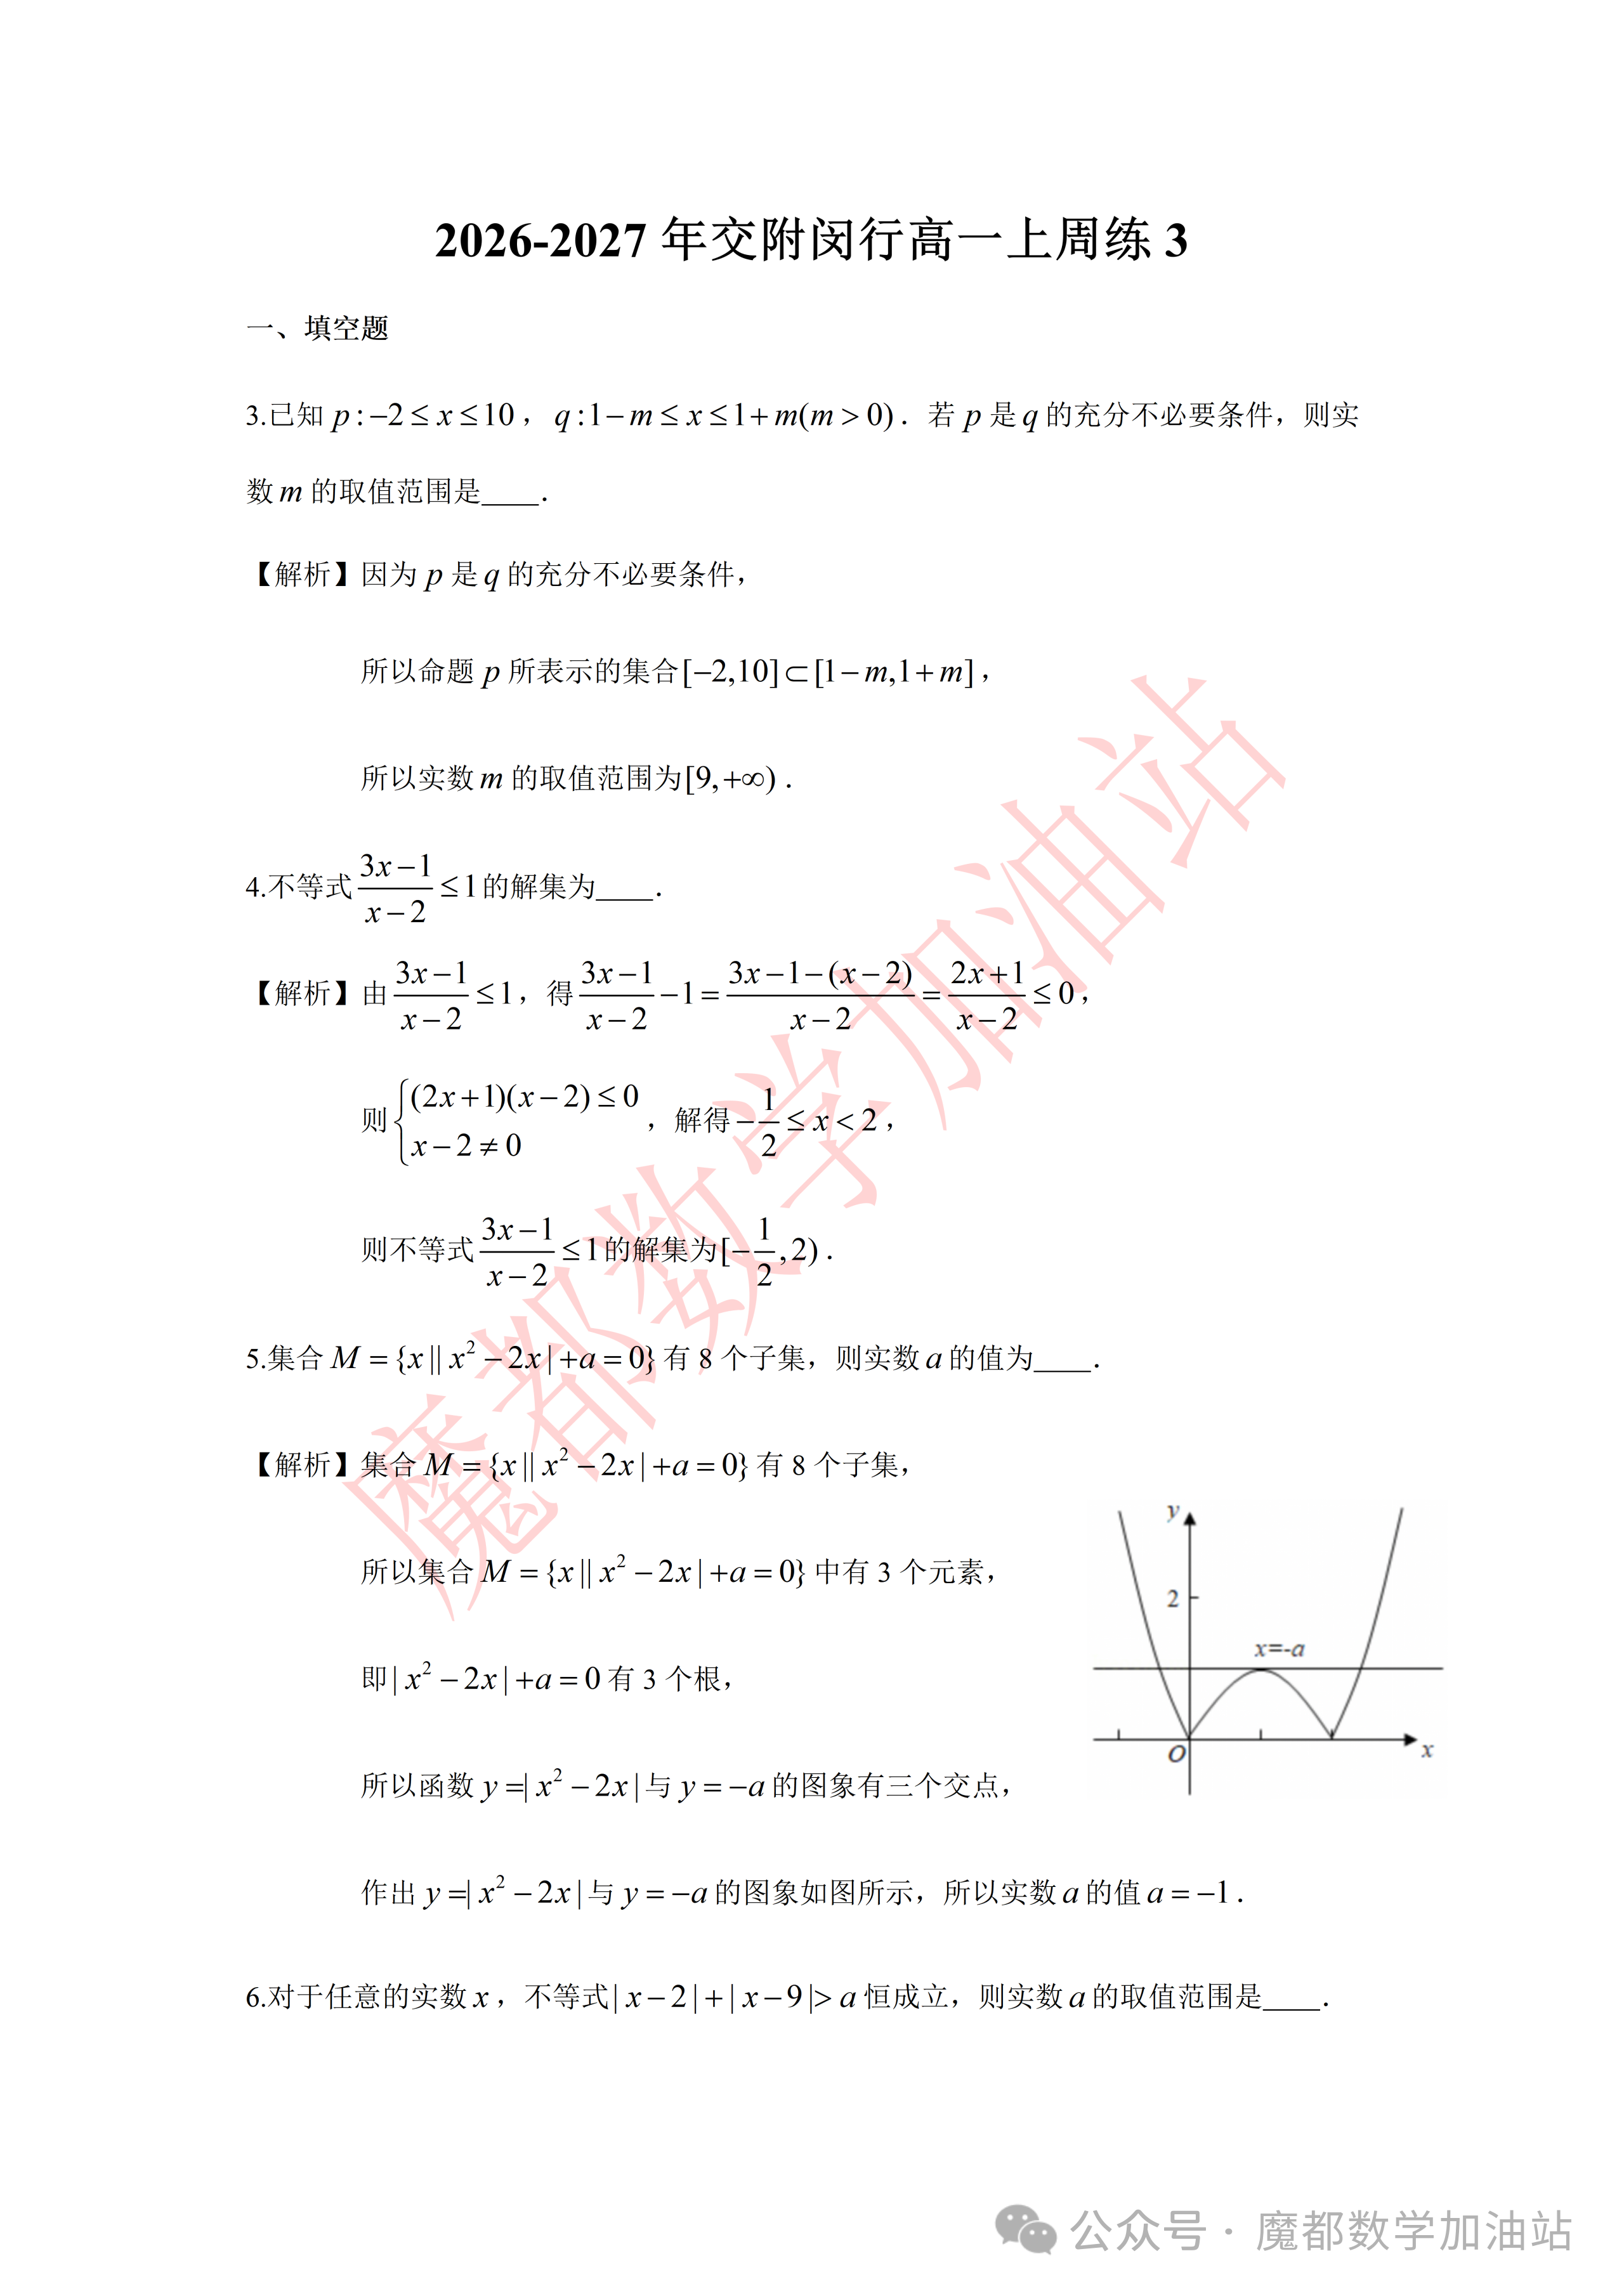
\includegraphics[width=0.14\textwidth,trim={1721bp 837bp 280bp 2297bp},clip]{../原图/高一43_交附闵行_周练3/01.png}
\end{center}

\solbegin
\step{集合 $M=\{x\mid |x^2-2x|+a=0\}$ 有 8 个子集，}
\step{所以集合 $M=\{x\mid |x^2-2x|+a=0\}$ 中有 3 个元素，}
\step{即 $|x^2-2x|+a=0$ 有 3 个根，}
\step{所以函数 $y=|x^2-2x|$ 与 $y=-a$ 的图象有三个交点，}
\step{作出 $y=|x^2-2x|$ 与 $y=-a$ 的图象如图所示，所以实数 $a$ 的值 $a=-1$.}
\solend

\fi

\item 对于任意的实数 $x$，不等式 $|x-2|+|x-9|>a$ 恒成立，则实数 $a$ 的取值范围是 \blankline[4.4em].

\ifanswer
\solbegin
\step{由绝对值的几何意义得 $|x-2|+|x-9|\geqslant7$，当且仅当 $2\leqslant x\leqslant9$ 时等号成立，}
\step{所以 $a<7$，}
\step{即 $a$ 的取值范围为 $(-\infty,7)$.}
\solend

\fi

\item 已知集合 $A=\{x\mid(a-1)x^2+3x-2=0\}$，$B=\{x\mid x^2-3x+2=0\}$，$A\subseteq B$，求实数 $a$ 的取值范围是 \blankline[4.4em].

\ifanswer
\solbegin
\step{由方程 $x^2-3x+2=0$，解得 $x=1$ 或 $x=2$，即 $B=\{1,2\}$，}
\step{因为 $A\subseteq B$，所以 $A=\varnothing$ 或 $A=\{1\}$ 或 $A=\{2\}$ 或 $A=\{1,2\}$，}
\step{当 $A=\varnothing$ 时，$a\neq1$，且 $\Delta=3^2-4(a-1)\times(-2)<0$，解得 $a<-\dfrac18$，}
\step{将 $x=1$ 代入方程 $(a-1)x^2+3x-2=0$，得 $a=0$，}
\step{此时 $A=\{x\mid-x^2+3x-2=0\}=\{1,2\}$，满足条件，}
\step{将 $x=2$ 代入方程 $(a-1)x^2+3x-2=0$，得到 $a=0$，上面已经验证满足条件，}
\step{综上所述，$a$ 的取值范围是 $\left(-\infty,-\dfrac18\right)\cup\{0\}$.}
\solend

\fi

\item 已知 $a$、$b$、$c$、$d$ 为常数，若不等式
$\dfrac{b}{x+a}+\dfrac{x+d}{x+c}<0$ 的解集为 $\left(-1,-\dfrac13\right)\cup\left(\dfrac12,1\right)$，
则不等式 $\dfrac{bx}{ax-1}+\dfrac{dx-1}{cx-1}<0$ 的解集为 \blankline[4.4em].

\ifanswer
\solbegin
\step{若 $x=0$，原不等式化为 $1<0$，不等式显然不成立，所以 $x\neq0$，}
\step{由 $\dfrac{bx}{ax-1}+\dfrac{dx-1}{cx-1}<0$，得 $\dfrac{b}{a-\dfrac1x}+\dfrac{d-\dfrac1x}{c-\dfrac1x}<0$，即 $\dfrac{b}{-\dfrac1x+a}+\dfrac{-\dfrac1x+d}{-\dfrac1x+c}<0$.}
\step{因为不等式 $\dfrac{b}{x+a}+\dfrac{x+d}{x+c}<0$ 的解集为 $\left(-1,-\dfrac13\right)\cup\left(\dfrac12,1\right)$，}
\step{所以 $-1<-\dfrac1x<-\dfrac13$ 或 $\dfrac12<-\dfrac1x<1$，解得 $1<x<3$ 或 $-2<x<-1$，}
\step{所以不等式 $\dfrac{bx}{ax-1}+\dfrac{dx-1}{cx-1}<0$ 的解集为 $(-2,-1)\cup(1,3)$.}
\solend

\fi

\item 正实数 $x$、$y$ 满足 $2x+3y-xy=0$，且存在这样的 $x$、$y$ 使不等式 $x+y<m+1$ 有解，则实数 $m$ 的取值范围是 \blankline[4.4em].

\ifanswer
\solbegin
\step{因为正实数 $x$、$y$ 满足 $2x+3y-xy=0$，则 $\dfrac2y+\dfrac3x=1$，$x>0$，$y>0$，}
\step{所以 $x+y=(x+y)\left(\dfrac3x+\dfrac2y\right)=3+\dfrac{2x}{y}+\dfrac{3y}{x}+2\geqslant2\sqrt{\dfrac{2x}{y}\times\dfrac{3y}{x}}+5=5+2\sqrt6$，}
\step{当且仅当 $\sqrt2x=\sqrt3y$ 时取等号，}
\step{存在这样的 $x$、$y$ 使不等式 $x+y<m+1$ 有解，则 $m+1>5+2\sqrt6$，}
\step{则 $m>4+2\sqrt6$，所以实数 $m$ 的取值范围是 $(4+2\sqrt6,+\infty)$.}
\solend

\fi

\item 若 $a$、$b$、$c\in\R$，$a^2+b^2+c^2=1$，则 $2ab+bc$ 的最大值为 \blankline[4.4em].

\ifanswer
\solbegin
\step{对于 $2ab+bc$，将 $b^2$ 拆分为 $\dfrac45b^2+\dfrac15b^2$，则 $a^2+\dfrac45b^2+c^2+\dfrac15b^2=1$，}
\step{$a^2+\dfrac45b^2\geqslant2\cdot a\cdot\dfrac2{\sqrt5}b=\dfrac4{\sqrt5}ab$，$c^2+\dfrac15b^2\geqslant2\cdot c\cdot\dfrac1{\sqrt5}b=\dfrac2{\sqrt5}bc$，}
\step{两式相加得 $1\geqslant\dfrac4{\sqrt5}ab+\dfrac2{\sqrt5}bc=\dfrac2{\sqrt5}(2ab+bc)$，故 $2ab+bc\leqslant\dfrac{\sqrt5}2$，}
\step{等号成立当且仅当 $a=\dfrac2{\sqrt5}b$，$c=\dfrac1{\sqrt5}b$，}
\step{代入 $a^2+b^2+c^2=1$，得 $\dfrac45b^2+b^2+\dfrac15b^2=2b^2=1$，即 $b=\dfrac{\sqrt2}2$，}
\step{此时 $a=\dfrac{\sqrt{10}}5$，$c=\dfrac{\sqrt{10}}{10}$，故 $2ab+bc$ 的最大值为 $\dfrac{\sqrt5}2$.}
\solend

\fi

\item 已知实数 $a$、$b$ 满足 $-3<a+2b<2$，$-1<2a-b<4$，则 $a+b$ 的取值范围为 \blankline[4.4em].

\ifanswer
\solbegin
\step{设 $a+b=m(a+2b)+n(2a-b)=(m+2n)a+(2m-n)b$，}
\step{所以 $\begin{cases}m+2n=1\\2m-n=1\end{cases}$，解得 $n=\dfrac15$，$m=\dfrac35$，所以 $a+b=\dfrac35(a+2b)+\dfrac15(2a-b)$，}
\step{因为 $-3<a+2b<2$，$-1<2a-b<4$，}
\step{所以 $-\dfrac95<\dfrac35(a+2b)<\dfrac65$，$-\dfrac15<\dfrac15(2a-b)<\dfrac45$，}
\step{相加得 $-2<\dfrac35(a+2b)+\dfrac15(2a-b)<2$，即 $-2<a+b<2$，}
\step{故 $a+b$ 的取值范围为 $(-2,2)$.}
\solend

\fi

% 注：原卷题干与解析均印作 \sqrt{2xyz}，但按其自身答案 8 与取等值（$y=\dfrac12$，
% $x=\dfrac{\sqrt3}4$，$z=\dfrac{\sqrt6}4$）代入只与 $\sqrt{2x^2y^2z^2}=\sqrt2\,xyz$ 相符，
% $\sqrt{2xyz}$ 与答案 8 不自洽，原卷如此，照录未改。
\item 已知正数 $x$、$y$、$z$ 满足 $2x^2+y^2+z^2=1$，则 $\dfrac{y+1}{\sqrt{2xyz}}$ 的最小值为 \blankline[4.4em].

\ifanswer
\solbegin
\step{由条件得 $2x^2+z^2=1-y^2=(1-y)(1+y)$，则 $1+y=\dfrac{2x^2+z^2}{1-y}$，}
\step{结合 $x$、$y$、$z>0$ 得原式 $=\dfrac{2x^2+z^2}{\sqrt{2xyz}(1-y)}\geqslant\dfrac{2\sqrt2xz}{\sqrt{2xyz}(1-y)}=\dfrac2{y(1-y)}$，}
\step{又 $y(1-y)\leqslant\left(\dfrac{y+1-y}2\right)^2=\dfrac14$，所以 $\dfrac2{y(1-y)}\geqslant\dfrac2{\frac14}=8$，}
\step{当且仅当 $\sqrt2x=z$，且 $y=1-y$，即 $y=\dfrac12$，$x=\dfrac{\sqrt3}4$，$z=\dfrac{\sqrt6}4$ 时取等号，}
\step{故 $\dfrac{y+1}{\sqrt{2xyz}}$ 最小值为 $8$.}
\solend

\fi

\end{enumerate}

\bigsec{二、选择题}

\begin{enumerate}
\setcounter{enumi}{12}

\item 已知关于 $x$ 的方程 $(1-k)x^2-2x-1=0$ 有实数根，则 $k$ 的取值范围是\mbox{（\quad）}

\keepwithprev
A. $k\leqslant2$ 且 $k\neq1$\qquad B. $k\leqslant2$\qquad
C. $k<2$ 且 $k\neq1$\qquad D. $k<2$

\ans{$A$}

\ifanswer
\solbegin
\step{由题意得 $\begin{cases}1-k\neq0\\\Delta=4+4(1-k)\geqslant0\end{cases}$，解不等式得 $\begin{cases}1\neq k\\2-k>0\end{cases}$，所以 $k\leqslant2$ 且 $k\neq1$，}
\step{故选 $A$.}
\solend

\fi

\item 不等式 $2|x+2|+|x-1|\geqslant5$ 成立的一个必要不充分条件是\mbox{（\quad）}

\keepwithprev
A. $x\leqslant-1$ 或 $x\geqslant0$\qquad B. $x\geqslant0$

C. $x\leqslant-\dfrac83$ 或 $x\geqslant0$\qquad D. $x\geqslant1$

\ans{$A$}

\ifanswer
\solbegin
\step{当 $x<-2$ 时，原不等式可化为 $-2x-4-x+1\geqslant5$，解得 $x\leqslant-\dfrac83$，}
\step{当 $-2\leqslant x<1$ 时，原不等式可化为 $2x+4-x+1\geqslant5$，解得 $0\leqslant x<1$，}
\step{当 $x\geqslant1$ 时，原不等式可化为 $2x+4+x-1\geqslant5$，解得 $x\geqslant\dfrac23$，得 $x\geqslant1$，}
\step{综上所述，不等式 $2|x+2|+|x-1|\geqslant5$ 成立的充要条件是 $x\leqslant-\dfrac83$ 或 $x\geqslant0$，}
\step{设 $A=\{x\mid x\leqslant-\dfrac83\text{ 或 }x\geqslant0\}$，}
\step{则不等式 $2|x+2|+|x-1|\geqslant5$ 成立的必要不充分条件，}
\step{其对应的集合 $B$ 满足 $A\subsetneq B$，对照各个选项，$A$ 项符合题意. 故选 $A$.}
\solend

\fi

\item 已知实数 $a>0$，$b>0$，$\dfrac1{a+1}+\dfrac1{b+1}=1$，则 $2a+3b$ 的最小值为\mbox{（\quad）}

\keepwithprev
A. $2\sqrt6$\qquad B. $3+2\sqrt6$\qquad
C. $5+2\sqrt6$\qquad D. $3+2\sqrt2$

\ans{$A$}

\ifanswer
\solbegin
\step{因为 $a>0$，$b>0$，$\dfrac1{a+1}+\dfrac1{b+1}=1$，}
\step{所以 $2a+3b=2(a+1)+3(b+1)-5=[2(a+1)+3(b+1)]\cdot\left(\dfrac1{a+1}+\dfrac1{b+1}\right)-5$}
\step{$=\left[2+3+\dfrac{3(b+1)}{a+1}+\dfrac{2(a+1)}{b+1}\right]-5\geqslant5+2\sqrt{\dfrac{3(b+1)}{a+1}\times\dfrac{2(a+1)}{b+1}}-5=2\sqrt6$，}
\step{当且仅当 $\dfrac{3(b+1)}{a+1}=\dfrac{2(a+1)}{b+1}$，即 $a=\dfrac{\sqrt6}2$，$b=\dfrac{\sqrt6}3$ 时取等号. 故选 $A$.}
\solend

\fi

\item 已知集合 $U=\{n\mid1\leqslant n\leqslant2027,\ n\in\N\}$，集合 $M\subseteq U$，若对于 $M$ 中任意两个不同的元素 $x$ 和 $y$，都有 $|x-y|>2$，则 $M$ 中元素个数的最大值是\mbox{（\quad）}

\keepwithprev
A. $676$\qquad B. $675$\qquad C. $672$\qquad D. $671$

\ans{$A$}

\ifanswer
\solbegin
\step{对于 $M$ 中的任意两个不同的元素 $x$、$y$，都有 $|x-y|>2$，}
\step{不妨设 $x>y$，都有 $x-y\geqslant3$，}
\step{要想 $M$ 所含元素个数最大，则要 $x-y$ 尽可能小，故需使得 $x-y$ 的最小值为 3，}
\step{将 $1\sim2027$ 这 2027 个元素按如下分组：}
\step{$\{1,2,3\}$，$\{4,5,6\}$，$\cdots$，$\{2023,2024,2025\}$，$\{2026,2027\}$，}
\step{故应在前 675 组中按周期 3 每组取一个元素，且第一组中不能取 3，}
\step{第一组中取 1 时，得 $M=\{1,4,7,\cdots,2023,2026\}$，}
\step{或 $M=\{1,4,7,\cdots,2023,2027\}$ 这样的集合，}
\step{第一组取 2 时，得 $M=\{2,5,8,\cdots,2024,2027\}$，}
\step{其中任意两元素差值 $x-y$（$x>y$）都大于 2，满足题意，}
\step{故 $M$ 所含元素个数的最大值为 $\dfrac{2025}{3}+1=676$. 故选 $A$.}
\solend

\fi

\end{enumerate}

\bigsec{三、解答题}

\begin{enumerate}
\setcounter{enumi}{16}

\item 已知 $a\in\R$，集合 $A=\left\{x\middle|\dfrac{2-x}{x+1}\leqslant0\right\}$，$B=\{x\mid x^2+(3-a)x-3a<0\}$.

\begin{enumerate}[label=(\arabic*)]
\item 当 $a=\dfrac13$ 时，求 $A$ 和 $B$；
\item 已知 $A\cup B=A$，求实数 $a$ 的取值范围.
\end{enumerate}

\ifanswer
\solbegin
\stepm{(1)}{由 $\dfrac{2-x}{x+1}\leqslant0$，得 $\begin{cases}(2-x)(x+1)\leqslant0\\x\neq-1\end{cases}$，解得 $x<-1$ 或 $x\geqslant2$，}
\step{则 $A=\{x\mid x<-1\text{ 或 }x\geqslant2\}$；}
\step{$B=\{x\mid x^2+(3-a)x-3a<0\}=\{x\mid(x+3)(x-a)<0\}$，}
% 注：原卷此行印作 $(x+2)\left(x-\dfrac13\right)$，按前一行 $B=\{x\mid(x+3)(x-a)<0\}$ 应为
% $(x+3)\left(x-\dfrac13\right)$，原卷如此，照录未改。
\step{当 $a=\dfrac13$ 时，$B=\left\{x\middle|(x+2)\left(x-\dfrac13\right)<0\right\}$，}
\step{解得 $B=\left\{x\middle|-3<x<\dfrac13\right\}$.}
\stepm{(2)}{由 $A\cup B=A$，得 $B\subseteq A$，}
\step{①当 $B=\varnothing$ 时，得 $a=-3$，符合题意；}
\step{②当 $B\neq\varnothing$ 时，若 $a>-3$，则 $B=\{x\mid-3<x<a\}$，}
\step{由 $B\subseteq A$，得 $a\leqslant-1$，此时 $-3<a\leqslant-1$；}
\step{若 $a<-3$，则 $B=\{x\mid a<x<-3\}$，此时 $B\subseteq A$ 恒成立，}
\step{故 $a<-3$ 符合题意；}
\step{综上所述，实数 $a$ 的取值范围为 $a\leqslant-1$.}
\solend

\fi

\ansspace[6]

\item 甲乙两地的高速公路全长 166 千米，汽车从甲地进入该高速公路后匀速行驶到乙地，车速 $v\in[70,120]$（千米/时）. 已知汽车每小时的运输成本（以元为单位）由可变部分和固定部分组成：可变部分为 $0.02v^2$，固定部分为 220 元.

\begin{enumerate}[label=(\arabic*)]
\item 若每小时的运输成本不高于 420 元，汽车的速度应该控制在什么范围？
\item 汽车应以多大速度行驶才能使全程运输成本最小？最小运输成本约为多少元？（结果保留整数）
\end{enumerate}

\ifanswer
\solbegin
\stepm{(1)}{已知汽车每小时的运输成本（以元为单位）由可变部分和固定部分组成：}
\step{可变部分为 $0.02v^2$，固定部分为 220 元，}
\step{则汽车每小时的运输成本为 $0.02v^2+220$（元），}
\step{若每小时的运输成本不高于 420 元，}
\step{则 $0.02v^2+220\leqslant420$，解得 $v^2\leqslant10000$，}
\step{得 $70\leqslant v\leqslant100$，即 $v\in[70,100]$（千米/时），}
\step{则此时汽车的速度 $v$ 应该控制在 $[70,100]$（千米/时）；}
\stepm{(2)}{因为汽车从甲地进入该高速公路后匀速行驶到乙地，}
\step{车速 $v\in[70,120]$（千米/时），所以汽车的行驶时间为 $\dfrac{166}{v}$（小时），}
\step{所以全程运输成本 $y=\dfrac{166}{v}(0.02v^2+220)=3.32v+\dfrac{36520}{v}$，}
% 注：原卷此行印作 $v\in[70,100]$，与题干的 $v\in[70,120]$ 不自洽（若 $v\in[70,100]$，
% 最小值应在 $v=100$ 处取得，与下文 $v=10\sqrt{110}\approx105$ 矛盾），原卷如此，照录未改。
\step{$v\in[70,100]$，}
\step{由基本不等式得 $y=3.32v+\dfrac{36520}{v}\geqslant2\sqrt{3.32v\times\dfrac{36520}{v}}\approx696$，}
\step{当且仅当 $3.32v=\dfrac{36520}{v}$，即 $v=10\sqrt{110}\approx105$ 时取等号，}
\step{汽车应以 105（千米/时）行驶才能使全程运输成本最小，}
\step{最小运输成本约为 696 元.}
\solend

\fi

\ansspace[8]

\item
\begin{enumerate}[label=(\arabic*)]
\item 已知 $a$、$b$、$c$ 为实数，求证：$|a-b|\leqslant|a-c|+|b-c|$，并说明等号成立的条件；
\item 设 $x\in\R$，求方程 $|3x-8|=|5-x|+|2x-3|$ 的解集.
\end{enumerate}

\ifanswer
% 注：原卷第 19 题未印【解析】，仅印一行【答案】"（1）(a-c)(b-c)≤0；
% （2）(-∞,3/2]∪[5,+∞)"。(1) 的两行推导为本稿所补，(2) 照录原卷答案。
% 又题干作"方程"，而所给答案 (-∞,3/2]∪[5,+∞) 实为不等式 |3x-8|≤|5-x|+|2x-3| 的解集，
% 与"方程"不合，原卷如此，照录未改。
\solbegin
\stepm{(1)}{由三角不等式 $|a-b|=|(a-c)-(b-c)|\leqslant|a-c|+|b-c|$，}
\step{当且仅当 $(a-c)(b-c)\leqslant0$ 时等号成立.}
\stepm{(2)}{$\left(-\infty,\dfrac32\right]\cup[5,+\infty)$.}
\solend

\fi

\ansspace[6]

\item 已知正实数 $a$、$b$ 满足 $a+b=1$，求 $\dfrac1a+\dfrac1b$ 的最小值. 其中一种解法是：

\[
\begin{aligned}
\dfrac1a+\dfrac1b
&=\left(\dfrac1a+\dfrac1b\right)(a+b)\\
&=1+\dfrac ba+\dfrac ab+1\\
&\geqslant2+2\sqrt{\dfrac ba\times\dfrac ab}=2+2=4.
\end{aligned}
\]
当且仅当 $\dfrac ba=\dfrac ab$ 且 $a+b=1$ 时即 $a=b=\dfrac12$ 时取等号.
学习上述解法并解决下列问题：

\begin{enumerate}[label=(\arabic*)]
\item 若正实数 $x$、$y$ 满足 $x+y=xy$，求 $2x+y$ 的最小值；
\item 若实数 $a$、$b$、$x$、$y$ 满足 $\dfrac{x^2}{a^2}+\dfrac{y^2}{b^2}=1$，求证：$a^2+b^2\geqslant(x+y)^2$；
\item 求代数式 $M=\sqrt{m-1}+\sqrt{3-m}$ 的最大值，并求出使得 $M$ 最大的 $m$ 的值.
\end{enumerate}

\ifanswer
\solbegin
\stepm{(1)}{因为正实数 $x$、$y$ 满足 $x+y=xy$，$\dfrac{x+y}{xy}=1\Rightarrow\dfrac1y+\dfrac1x=1$，}
\step{所以 $(2x+y)\times1=(2x+y)\left(\dfrac1y+\dfrac1x\right)=3+\dfrac{2x}{y}+\dfrac yx\geqslant3+2\sqrt{\dfrac{2x}{y}\cdot\dfrac yx}=3+2\sqrt2$，}
\step{当且仅当 $\dfrac{2x}{y}=\dfrac yx$ 且 $\dfrac1y+\dfrac1x=1$ 时取等号，}
\step{解得 $x=\dfrac{2+\sqrt2}2$，$y=\sqrt2x=\sqrt2\times\dfrac{2+\sqrt2}2=1+\sqrt2$，}
\step{所以 $2x+y$ 的最小值为 $3+2\sqrt2$；}
\stepm{(2)}{因为 $\dfrac{x^2}{a^2}+\dfrac{y^2}{b^2}=1$，}
\step{所以 $a^2+b^2=(a^2+b^2)\left(\dfrac{x^2}{a^2}+\dfrac{y^2}{b^2}\right)=x^2+y^2+\dfrac{b^2x^2}{a^2}+\dfrac{a^2y^2}{b^2}$，}
\step{因为 $\dfrac{b^2x^2}{a^2}+\dfrac{a^2y^2}{b^2}\geqslant2\sqrt{\dfrac{b^2x^2}{a^2}\times\dfrac{a^2y^2}{b^2}}=2\sqrt{x^2y^2}=2|xy|$，}
\step{当且仅当 $\dfrac{b^2x^2}{a^2}=\dfrac{a^2y^2}{b^2}$ 时取等号，}
\step{所以 $x^2+y^2+\dfrac{b^2x^2}{a^2}+\dfrac{a^2y^2}{b^2}\geqslant x^2+y^2+2|xy|\geqslant x^2+y^2+2xy=(x+y)^2$，}
\step{所以 $a^2+b^2\geqslant(x+y)^2$；}
\stepm{(3)}{因为 $M=\sqrt{m-1}+\sqrt{3-m}$，所以 $\begin{cases}m-1\geqslant0\\3-m\geqslant0\end{cases}$，解得 $1\leqslant m\leqslant3$，}
\step{所以 $M^2=(\sqrt{m-1}+\sqrt{3-m})^2=2+2\sqrt{(3-m)(m-1)}$，}
\step{由基本不等式得 $(3-m)(m-1)\leqslant\left(\dfrac{(3-m)+(m-1)}2\right)^2=1$，}
\step{当且仅当 $3-m=m-1$ 时取等号，解得 $m=2$，}
\step{所以 $M^2=2+2\sqrt{(3-m)(m-1)}\leqslant2+2\sqrt1=4$，}
\step{因为 $M>0$，所以 $M\leqslant2$，所以 $M$ 最大值为 2，此时 $m$ 的值为 2.}
\solend

\fi

\ansspace[8]

\item 若有限个正整数组成的集合 $A$ 中至少有两个元素，且对于任意的 $x,y\in A$（$x>y$），都有 $\dfrac{y^2}{x-y}\in A$，则称 $A$ 为“L-集合”.

\begin{enumerate}[label=(\arabic*)]
\item 判断 $\{1,2,4\}$ 是否为“L-集合”，说明理由；
\item 若双元素集 $M$ 为“L-集合”，且 $4\in M$，求所有满足条件的集合 $M$；
\item 求所有满足条件的“L-集合”.
\end{enumerate}

\ifanswer
\solbegin
\stepm{(1)}{若至少由两个元素构成的有限集合 $A\subseteq\N^*$，}
% 注：原卷下一行"都有"后未印分数 \dfrac{y^2}{x-y}，径作"都有 A"，原卷如此，照录未改。
\step{且对于任意的 $x$、$y\in A$（$x>y$），都有 $A$，则称 $A$ 为“L-集合”，}
\step{$\{1,2,4\}$ 不为“L-集合”，理由如下：}
\step{因为 $\dfrac{1^2}{4-1}=\dfrac13\notin\{1,2,4\}$，所以 $\{1,2,4\}$ 不是“L-集合”.}
\stepm{(2)}{设 $M=\{4,m\}$（$m\in\N^*$，$m\neq4$），}
\step{若 $m<4$，则 $\dfrac{m^2}{4-m}=m$ 或 $\dfrac{m^2}{4-m}=4$，}
\step{由 $\dfrac{m^2}{4-m}=m$，解得 $m=2$，$m=0$（舍去），此时 $M=\{2,4\}$；}
\step{由 $\dfrac{m^2}{4-m}=4$ 化为 $m^2+4m-16=0$，而 $\Delta=4^2+4\times16=80$，}
\step{故方程无正整数解.}
\step{若 $m>4$，则 $\dfrac{4^2}{m-4}=4$ 或 $\dfrac{4^2}{m-4}=m$，}
\step{由 $\dfrac{4^2}{m-4}=4$，解得 $m=8$，此时 $M=\{4,8\}$；}
\step{由 $\dfrac{4^2}{m-4}=m$ 化为 $m^2-4m-16=0$，而 $\Delta=4^2+4\times16=80$，}
\step{故方程无正整数解.}
\step{综上，双元素集 $M$ 为“L-集合”，且 $4\in M$，}
\step{则所有满足条件的集合 $M$ 为 $\{4,8\}$，$\{2,4\}$.}
\stepm{(3)}{若“L-集合”为双元素集，}
\step{不妨设 $M=\{k,m\}$（$k,m\in\N^*$，$m>k$），则 $\dfrac{k^2}{m-k}=k$ 或 $\dfrac{k^2}{m-k}=m$，}
\step{由 $\dfrac{k^2}{m-k}=k$，则 $2k^2=mk$，而 $m>k$，故 $m=2k$，此时 $M=\{k,2k\}$；}
\step{由 $\dfrac{k^2}{m-k}=m$，则 $m^2-mk-k^2=0$，而 $\Delta=5k^2$，显然不存在正整数解；}
\step{所以，“L-集合”为 $\{k,2k\}$，其中 $k\in\N^*$.}
\step{若“L-集合”含有两个以上的元素，}
\step{设最小的元素为 $b$，最大的元素为 $a$，第二大的元素为 $n$，}
\step{则 $\dfrac{b^2}{a-b}$，$\dfrac{n^2}{a-n}$ 是“L-集合”中的元素，}
% 注：原卷下一行未印"由于'L-集合'中的元素均为正整数"一语，径作"若 \dfrac{b^2}{a-b}\geqslant b"，
% 原卷如此，照录未改。
\step{若 $\dfrac{b^2}{a-b}\geqslant b$，解得 $a\leqslant2b$，}
\step{若 $\dfrac{n^2}{a-n}\leqslant n$，则 $a\geqslant2n>2b$，矛盾，}
\step{若 $\dfrac{n^2}{a-n}=a$，该方程的解为 $n=\dfrac{\sqrt5-1}2a$，则 $n$、$a$ 不可能同时为整数，}
\step{无解.}
\step{所以所有满足条件的“L-集合”为 $\{k,2k\}$，其中 $k\in\N^*$.}
\solend

\fi

\ansspace*[10]

\end{enumerate}

\end{document}
"
%
% 原始材料是微信公众号图文（公众号“魔都数学加油站”，作者破晓，2026-10-01 21:37，
% 原文标题“27学年高一43——2026-2027年上海市交附闵行高一上周练3”，
% https://mp.weixin.qq.com/s/-rgkOD9jJVpug6s0uSbwmQ）。正文为 12 张 PNG 页；
% 第 01、05、09、12 页 2560×3620，其余第 02—04、06—08、10—11 页 4762×6735。
% 原文本身是讲评版，题目下方印有解析/答案；题目与讲解照原卷转录，保留原卷错误。
%
% 卷首标题：原卷印作“2026-2027 年交附闵行高一上周练3”，公众号标题中的“上海市”
% 三字不在卷面标题中，本稿依卷面录入；年份区间按全稿惯例排 en dash。
%
% 与原卷的排版差异：
%   ① 原文从第 3 题开始（第 1、2 题未在这篇推文中发布），本稿保留原题号 3—21；
%   ② 原卷本就印有“一、填空题”“二、选择题”“三、解答题”，本稿照原卷分节，
%      改排为全稿统一的大节标题；
%   ③ 原卷未印副标题，本稿按“知识模块”口径补出“集合与常用逻辑用语、不等式”；
%   ④ 原卷填空横线依全稿惯例排为 \blankline[4.4em]；选择题答案只在答案版以 \ans{} 显示，
%      解答区以 \ifanswer 分离；解答题按原卷留出标准作答空间；
%   ⑤ 第 5 题图取自原卷第 1 页截图并裁入本稿，不另建图档；公众号水印不录入。
%      原卷图页分页不保留，正文依本稿版心重新分页。
%
% 原卷存疑/错误（均照录，未改）：
%   ① 第 9 题原卷题干即作"正实数 x、y"，与解析 x>0、y>0 相容，并无矛盾（初稿曾误记
%      题干只称"实数"并据此指原卷不自洽，2026-10-05 回原图核对订正）。
%   ② 第 11 题解析"相加得"一行原卷印作 -2<3/5(a+2b)+1/5(2a-b)<2，第一项系数 3/5
%      原卷不缺（初稿漏抄致该行按字面不成立，2026-10-05 已按原卷补回）。
%   ③ 第 13 题答案印 A，解析以“1-k≠0”排除 k=1；但 k=1 时原方程为 -2x-1=0，
%      仍有实数根，按题意应选 B。本稿保留原卷答案 A 及其解析，不代为订正。
%
\documentclass[a4paper,11pt]{article}
\usepackage{common}
\usepackage{graphicx}

\begin{document}

\examtitlest[3]{2026--2027 年交附闵行高一上周练 3}{集合与常用逻辑用语、不等式}

\bigsec{一、填空题}

\begin{enumerate}
\setcounter{enumi}{2}

\item 已知 $p\colon -2\leqslant x\leqslant10$，$q\colon 1-m\leqslant x\leqslant1+m$（$m>0$）. 若 $p$ 是 $q$ 的充分不必要条件，则实数 $m$ 的取值范围是 \blankline[4.4em].

\ifanswer
\solbegin
\step{因为 $p$ 是 $q$ 的充分不必要条件，}
\step{所以命题 $p$ 所表示的集合 $[-2,10]\subset[1-m,1+m]$，}
\step{所以实数 $m$ 的取值范围为 $[9,+\infty)$.}
\solend

\fi

\item 不等式 $\dfrac{3x-1}{x-2}\leqslant1$ 的解集为 \blankline[4.4em].

\ifanswer
\solbegin
\step{由 $\dfrac{3x-1}{x-2}-1=\dfrac{3x-1-(x-2)}{x-2}=\dfrac{2x+1}{x-2}\leqslant0$，}
\step{则 $\begin{cases}(2x+1)(x-2)\leqslant0\\x-2\neq0\end{cases}$，解得 $-\dfrac12\leqslant x<2$，}
\step{则不等式 $\dfrac{3x-1}{x-2}\leqslant1$ 的解集为 $\left[-\dfrac12,2\right)$.}
\solend

\fi

\item 集合 $M=\{x\mid |x^2-2x|+a=0\}$ 有 8 个子集，则实数 $a$ 的值为 \blankline[4.4em].

\ifanswer
\begin{center}
% 图取自原卷第 1 页；用原图裁切，未重绘。
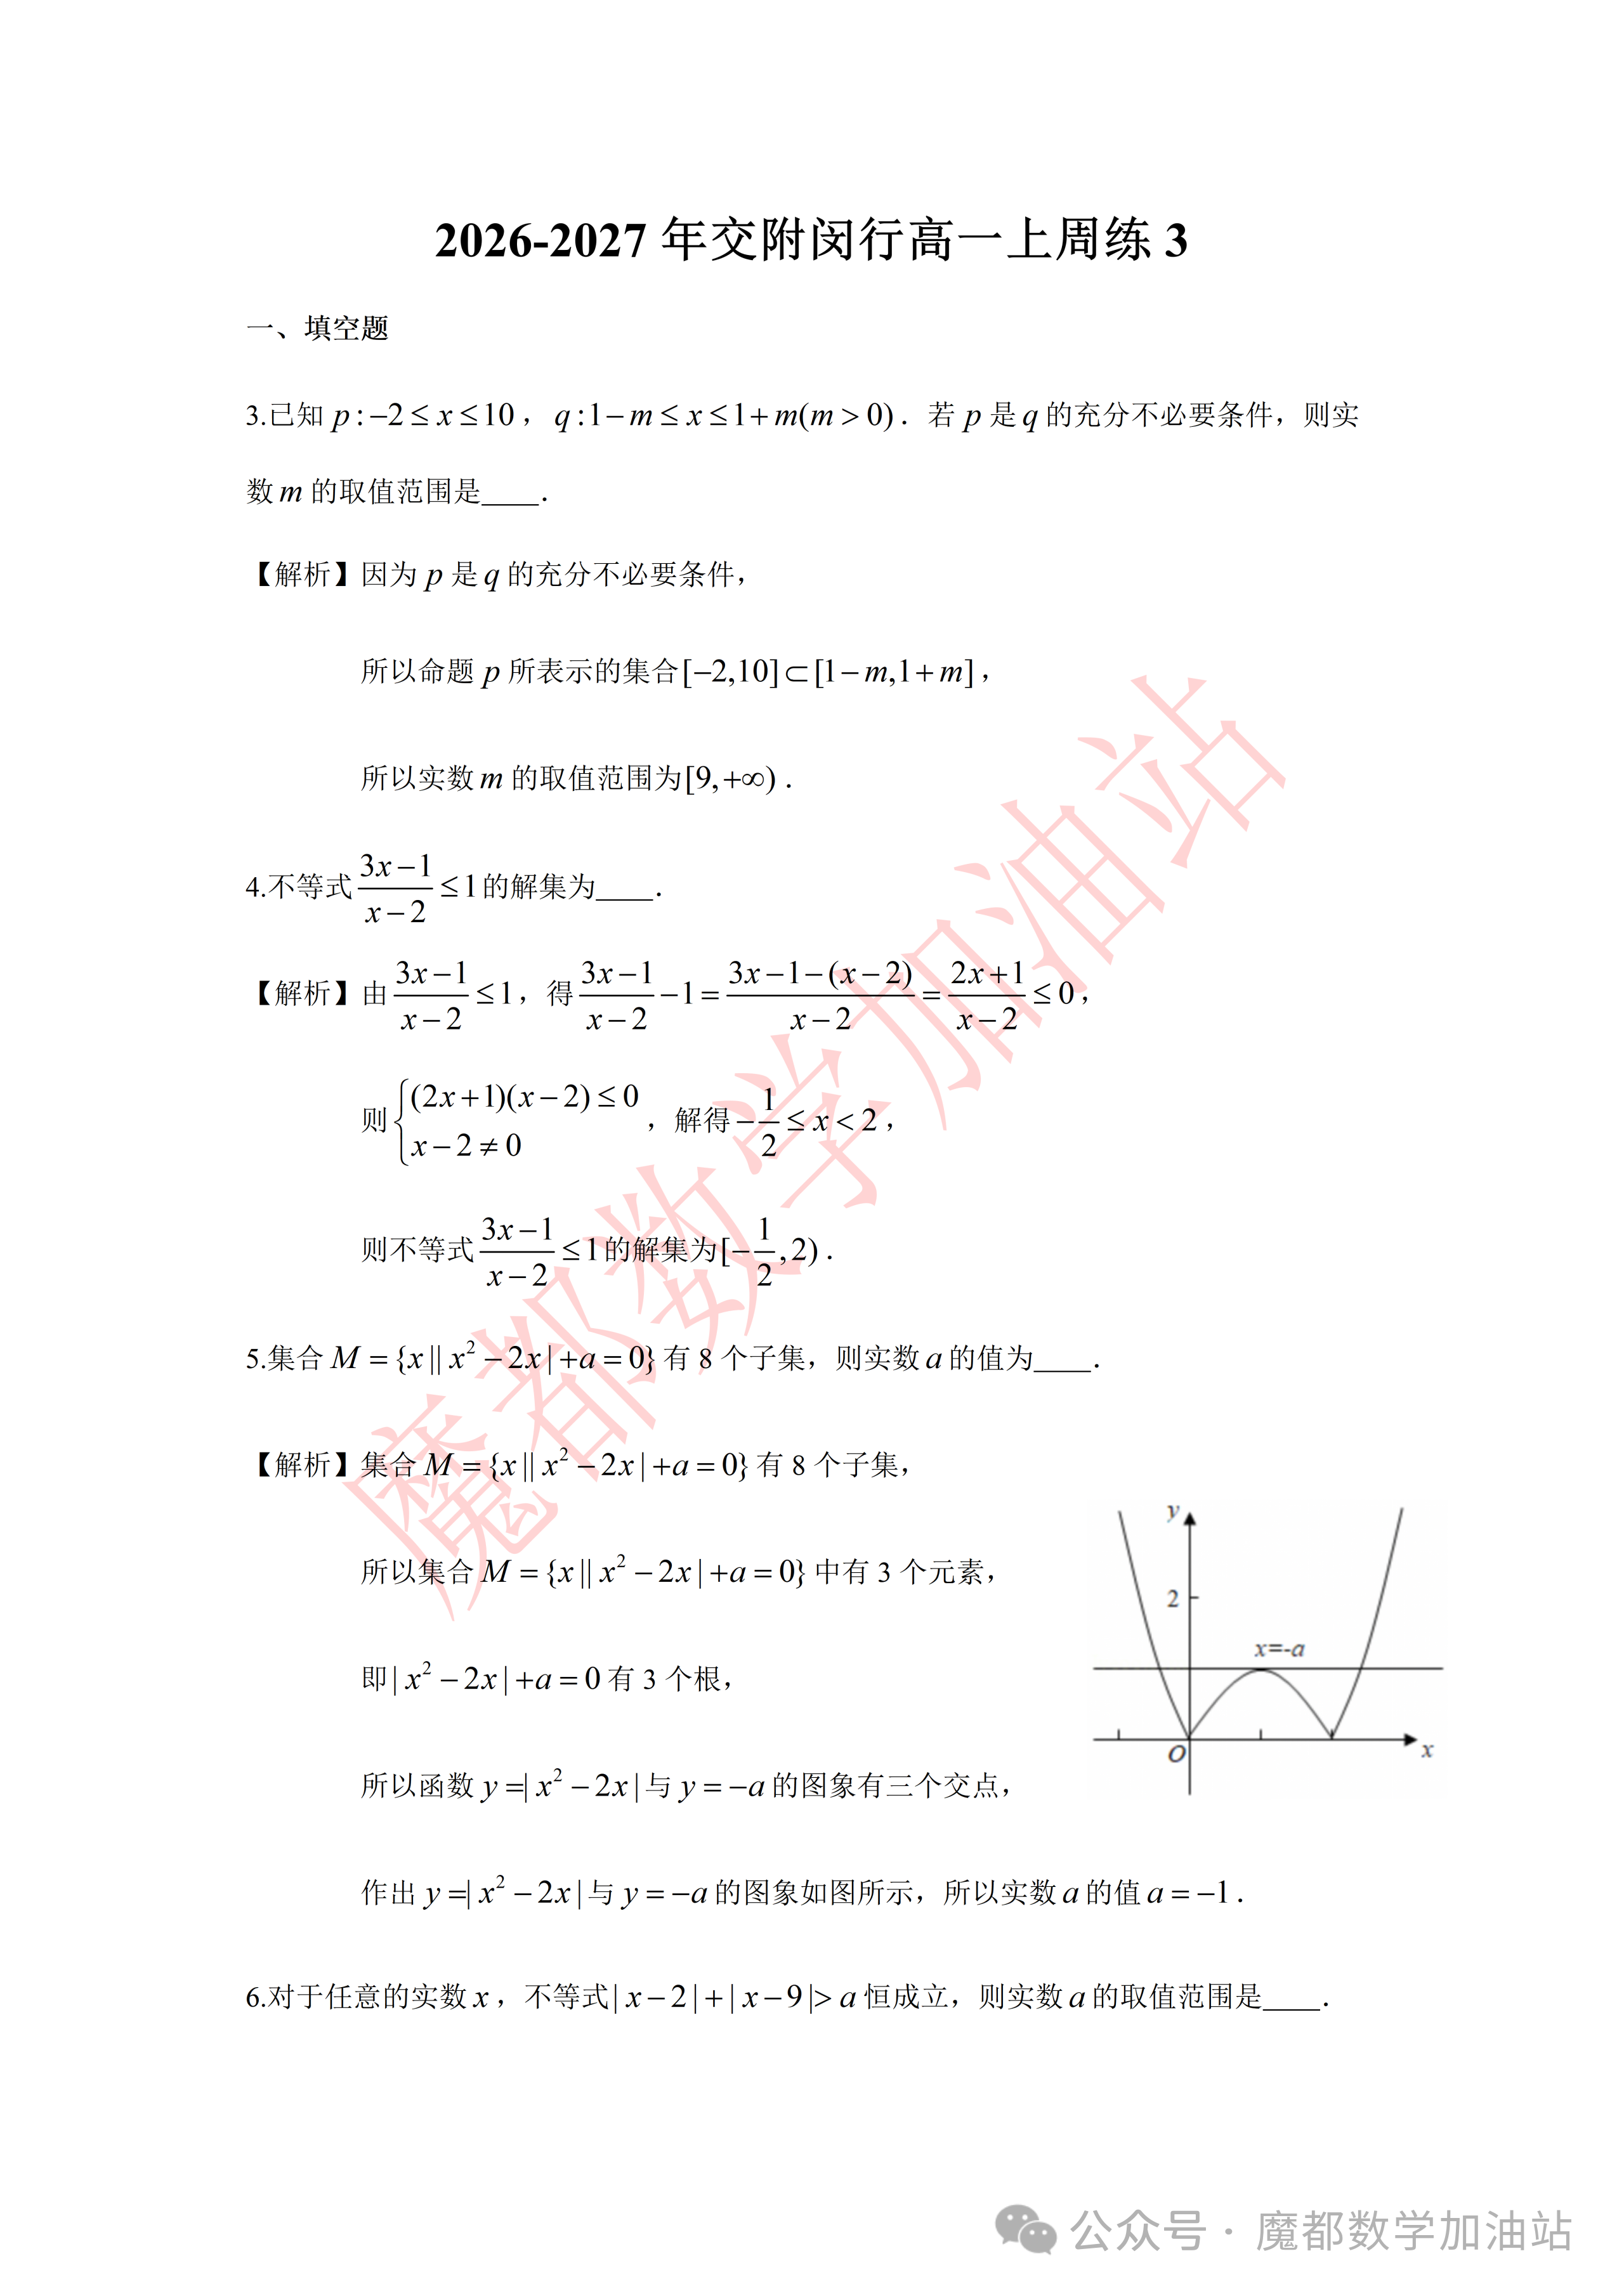
\includegraphics[width=0.14\textwidth,trim={1721bp 837bp 280bp 2297bp},clip]{../原图/高一43_交附闵行_周练3/01.png}
\end{center}

\solbegin
\step{集合 $M=\{x\mid |x^2-2x|+a=0\}$ 有 8 个子集，}
\step{所以集合 $M=\{x\mid |x^2-2x|+a=0\}$ 中有 3 个元素，}
\step{即 $|x^2-2x|+a=0$ 有 3 个根，}
\step{所以函数 $y=|x^2-2x|$ 与 $y=-a$ 的图象有三个交点，}
\step{作出 $y=|x^2-2x|$ 与 $y=-a$ 的图象如图所示，所以实数 $a$ 的值 $a=-1$.}
\solend

\fi

\item 对于任意的实数 $x$，不等式 $|x-2|+|x-9|>a$ 恒成立，则实数 $a$ 的取值范围是 \blankline[4.4em].

\ifanswer
\solbegin
\step{由绝对值的几何意义得 $|x-2|+|x-9|\geqslant7$，当且仅当 $2\leqslant x\leqslant9$ 时等号成立，}
\step{所以 $a<7$，}
\step{即 $a$ 的取值范围为 $(-\infty,7)$.}
\solend

\fi

\item 已知集合 $A=\{x\mid(a-1)x^2+3x-2=0\}$，$B=\{x\mid x^2-3x+2=0\}$，$A\subseteq B$，求实数 $a$ 的取值范围是 \blankline[4.4em].

\ifanswer
\solbegin
\step{由方程 $x^2-3x+2=0$，解得 $x=1$ 或 $x=2$，即 $B=\{1,2\}$，}
\step{因为 $A\subseteq B$，所以 $A=\varnothing$ 或 $A=\{1\}$ 或 $A=\{2\}$ 或 $A=\{1,2\}$，}
\step{当 $A=\varnothing$ 时，$a\neq1$，且 $\Delta=3^2-4(a-1)\times(-2)<0$，解得 $a<-\dfrac18$，}
\step{将 $x=1$ 代入方程 $(a-1)x^2+3x-2=0$，得 $a=0$，}
\step{此时 $A=\{x\mid-x^2+3x-2=0\}=\{1,2\}$，满足条件，}
\step{将 $x=2$ 代入方程 $(a-1)x^2+3x-2=0$，得到 $a=0$，上面已经验证满足条件，}
\step{综上所述，$a$ 的取值范围是 $\left(-\infty,-\dfrac18\right)\cup\{0\}$.}
\solend

\fi

\item 已知 $a$、$b$、$c$、$d$ 为常数，若不等式
$\dfrac{b}{x+a}+\dfrac{x+d}{x+c}<0$ 的解集为 $\left(-1,-\dfrac13\right)\cup\left(\dfrac12,1\right)$，
则不等式 $\dfrac{bx}{ax-1}+\dfrac{dx-1}{cx-1}<0$ 的解集为 \blankline[4.4em].

\ifanswer
\solbegin
\step{若 $x=0$，原不等式化为 $1<0$，不等式显然不成立，所以 $x\neq0$，}
\step{由 $\dfrac{bx}{ax-1}+\dfrac{dx-1}{cx-1}<0$，得 $\dfrac{b}{a-\dfrac1x}+\dfrac{d-\dfrac1x}{c-\dfrac1x}<0$，即 $\dfrac{b}{-\dfrac1x+a}+\dfrac{-\dfrac1x+d}{-\dfrac1x+c}<0$.}
\step{因为不等式 $\dfrac{b}{x+a}+\dfrac{x+d}{x+c}<0$ 的解集为 $\left(-1,-\dfrac13\right)\cup\left(\dfrac12,1\right)$，}
\step{所以 $-1<-\dfrac1x<-\dfrac13$ 或 $\dfrac12<-\dfrac1x<1$，解得 $1<x<3$ 或 $-2<x<-1$，}
\step{所以不等式 $\dfrac{bx}{ax-1}+\dfrac{dx-1}{cx-1}<0$ 的解集为 $(-2,-1)\cup(1,3)$.}
\solend

\fi

\item 正实数 $x$、$y$ 满足 $2x+3y-xy=0$，且存在这样的 $x$、$y$ 使不等式 $x+y<m+1$ 有解，则实数 $m$ 的取值范围是 \blankline[4.4em].

\ifanswer
\solbegin
\step{因为正实数 $x$、$y$ 满足 $2x+3y-xy=0$，则 $\dfrac2y+\dfrac3x=1$，$x>0$，$y>0$，}
\step{所以 $x+y=(x+y)\left(\dfrac3x+\dfrac2y\right)=3+\dfrac{2x}{y}+\dfrac{3y}{x}+2\geqslant2\sqrt{\dfrac{2x}{y}\times\dfrac{3y}{x}}+5=5+2\sqrt6$，}
\step{当且仅当 $\sqrt2x=\sqrt3y$ 时取等号，}
\step{存在这样的 $x$、$y$ 使不等式 $x+y<m+1$ 有解，则 $m+1>5+2\sqrt6$，}
\step{则 $m>4+2\sqrt6$，所以实数 $m$ 的取值范围是 $(4+2\sqrt6,+\infty)$.}
\solend

\fi

\item 若 $a$、$b$、$c\in\R$，$a^2+b^2+c^2=1$，则 $2ab+bc$ 的最大值为 \blankline[4.4em].

\ifanswer
\solbegin
\step{对于 $2ab+bc$，将 $b^2$ 拆分为 $\dfrac45b^2+\dfrac15b^2$，则 $a^2+\dfrac45b^2+c^2+\dfrac15b^2=1$，}
\step{$a^2+\dfrac45b^2\geqslant2\cdot a\cdot\dfrac2{\sqrt5}b=\dfrac4{\sqrt5}ab$，$c^2+\dfrac15b^2\geqslant2\cdot c\cdot\dfrac1{\sqrt5}b=\dfrac2{\sqrt5}bc$，}
\step{两式相加得 $1\geqslant\dfrac4{\sqrt5}ab+\dfrac2{\sqrt5}bc=\dfrac2{\sqrt5}(2ab+bc)$，故 $2ab+bc\leqslant\dfrac{\sqrt5}2$，}
\step{等号成立当且仅当 $a=\dfrac2{\sqrt5}b$，$c=\dfrac1{\sqrt5}b$，}
\step{代入 $a^2+b^2+c^2=1$，得 $\dfrac45b^2+b^2+\dfrac15b^2=2b^2=1$，即 $b=\dfrac{\sqrt2}2$，}
\step{此时 $a=\dfrac{\sqrt{10}}5$，$c=\dfrac{\sqrt{10}}{10}$，故 $2ab+bc$ 的最大值为 $\dfrac{\sqrt5}2$.}
\solend

\fi

\item 已知实数 $a$、$b$ 满足 $-3<a+2b<2$，$-1<2a-b<4$，则 $a+b$ 的取值范围为 \blankline[4.4em].

\ifanswer
\solbegin
\step{设 $a+b=m(a+2b)+n(2a-b)=(m+2n)a+(2m-n)b$，}
\step{所以 $\begin{cases}m+2n=1\\2m-n=1\end{cases}$，解得 $n=\dfrac15$，$m=\dfrac35$，所以 $a+b=\dfrac35(a+2b)+\dfrac15(2a-b)$，}
\step{因为 $-3<a+2b<2$，$-1<2a-b<4$，}
\step{所以 $-\dfrac95<\dfrac35(a+2b)<\dfrac65$，$-\dfrac15<\dfrac15(2a-b)<\dfrac45$，}
\step{相加得 $-2<\dfrac35(a+2b)+\dfrac15(2a-b)<2$，即 $-2<a+b<2$，}
\step{故 $a+b$ 的取值范围为 $(-2,2)$.}
\solend

\fi

% 注：原卷题干与解析均印作 \sqrt{2xyz}，但按其自身答案 8 与取等值（$y=\dfrac12$，
% $x=\dfrac{\sqrt3}4$，$z=\dfrac{\sqrt6}4$）代入只与 $\sqrt{2x^2y^2z^2}=\sqrt2\,xyz$ 相符，
% $\sqrt{2xyz}$ 与答案 8 不自洽，原卷如此，照录未改。
\item 已知正数 $x$、$y$、$z$ 满足 $2x^2+y^2+z^2=1$，则 $\dfrac{y+1}{\sqrt{2xyz}}$ 的最小值为 \blankline[4.4em].

\ifanswer
\solbegin
\step{由条件得 $2x^2+z^2=1-y^2=(1-y)(1+y)$，则 $1+y=\dfrac{2x^2+z^2}{1-y}$，}
\step{结合 $x$、$y$、$z>0$ 得原式 $=\dfrac{2x^2+z^2}{\sqrt{2xyz}(1-y)}\geqslant\dfrac{2\sqrt2xz}{\sqrt{2xyz}(1-y)}=\dfrac2{y(1-y)}$，}
\step{又 $y(1-y)\leqslant\left(\dfrac{y+1-y}2\right)^2=\dfrac14$，所以 $\dfrac2{y(1-y)}\geqslant\dfrac2{\frac14}=8$，}
\step{当且仅当 $\sqrt2x=z$，且 $y=1-y$，即 $y=\dfrac12$，$x=\dfrac{\sqrt3}4$，$z=\dfrac{\sqrt6}4$ 时取等号，}
\step{故 $\dfrac{y+1}{\sqrt{2xyz}}$ 最小值为 $8$.}
\solend

\fi

\end{enumerate}

\bigsec{二、选择题}

\begin{enumerate}
\setcounter{enumi}{12}

\item 已知关于 $x$ 的方程 $(1-k)x^2-2x-1=0$ 有实数根，则 $k$ 的取值范围是\mbox{（\quad）}

\keepwithprev
A. $k\leqslant2$ 且 $k\neq1$\qquad B. $k\leqslant2$\qquad
C. $k<2$ 且 $k\neq1$\qquad D. $k<2$

\ans{$A$}

\ifanswer
\solbegin
\step{由题意得 $\begin{cases}1-k\neq0\\\Delta=4+4(1-k)\geqslant0\end{cases}$，解不等式得 $\begin{cases}1\neq k\\2-k>0\end{cases}$，所以 $k\leqslant2$ 且 $k\neq1$，}
\step{故选 $A$.}
\solend

\fi

\item 不等式 $2|x+2|+|x-1|\geqslant5$ 成立的一个必要不充分条件是\mbox{（\quad）}

\keepwithprev
A. $x\leqslant-1$ 或 $x\geqslant0$\qquad B. $x\geqslant0$

C. $x\leqslant-\dfrac83$ 或 $x\geqslant0$\qquad D. $x\geqslant1$

\ans{$A$}

\ifanswer
\solbegin
\step{当 $x<-2$ 时，原不等式可化为 $-2x-4-x+1\geqslant5$，解得 $x\leqslant-\dfrac83$，}
\step{当 $-2\leqslant x<1$ 时，原不等式可化为 $2x+4-x+1\geqslant5$，解得 $0\leqslant x<1$，}
\step{当 $x\geqslant1$ 时，原不等式可化为 $2x+4+x-1\geqslant5$，解得 $x\geqslant\dfrac23$，得 $x\geqslant1$，}
\step{综上所述，不等式 $2|x+2|+|x-1|\geqslant5$ 成立的充要条件是 $x\leqslant-\dfrac83$ 或 $x\geqslant0$，}
\step{设 $A=\{x\mid x\leqslant-\dfrac83\text{ 或 }x\geqslant0\}$，}
\step{则不等式 $2|x+2|+|x-1|\geqslant5$ 成立的必要不充分条件，}
\step{其对应的集合 $B$ 满足 $A\subsetneq B$，对照各个选项，$A$ 项符合题意. 故选 $A$.}
\solend

\fi

\item 已知实数 $a>0$，$b>0$，$\dfrac1{a+1}+\dfrac1{b+1}=1$，则 $2a+3b$ 的最小值为\mbox{（\quad）}

\keepwithprev
A. $2\sqrt6$\qquad B. $3+2\sqrt6$\qquad
C. $5+2\sqrt6$\qquad D. $3+2\sqrt2$

\ans{$A$}

\ifanswer
\solbegin
\step{因为 $a>0$，$b>0$，$\dfrac1{a+1}+\dfrac1{b+1}=1$，}
\step{所以 $2a+3b=2(a+1)+3(b+1)-5=[2(a+1)+3(b+1)]\cdot\left(\dfrac1{a+1}+\dfrac1{b+1}\right)-5$}
\step{$=\left[2+3+\dfrac{3(b+1)}{a+1}+\dfrac{2(a+1)}{b+1}\right]-5\geqslant5+2\sqrt{\dfrac{3(b+1)}{a+1}\times\dfrac{2(a+1)}{b+1}}-5=2\sqrt6$，}
\step{当且仅当 $\dfrac{3(b+1)}{a+1}=\dfrac{2(a+1)}{b+1}$，即 $a=\dfrac{\sqrt6}2$，$b=\dfrac{\sqrt6}3$ 时取等号. 故选 $A$.}
\solend

\fi

\item 已知集合 $U=\{n\mid1\leqslant n\leqslant2027,\ n\in\N\}$，集合 $M\subseteq U$，若对于 $M$ 中任意两个不同的元素 $x$ 和 $y$，都有 $|x-y|>2$，则 $M$ 中元素个数的最大值是\mbox{（\quad）}

\keepwithprev
A. $676$\qquad B. $675$\qquad C. $672$\qquad D. $671$

\ans{$A$}

\ifanswer
\solbegin
\step{对于 $M$ 中的任意两个不同的元素 $x$、$y$，都有 $|x-y|>2$，}
\step{不妨设 $x>y$，都有 $x-y\geqslant3$，}
\step{要想 $M$ 所含元素个数最大，则要 $x-y$ 尽可能小，故需使得 $x-y$ 的最小值为 3，}
\step{将 $1\sim2027$ 这 2027 个元素按如下分组：}
\step{$\{1,2,3\}$，$\{4,5,6\}$，$\cdots$，$\{2023,2024,2025\}$，$\{2026,2027\}$，}
\step{故应在前 675 组中按周期 3 每组取一个元素，且第一组中不能取 3，}
\step{第一组中取 1 时，得 $M=\{1,4,7,\cdots,2023,2026\}$，}
\step{或 $M=\{1,4,7,\cdots,2023,2027\}$ 这样的集合，}
\step{第一组取 2 时，得 $M=\{2,5,8,\cdots,2024,2027\}$，}
\step{其中任意两元素差值 $x-y$（$x>y$）都大于 2，满足题意，}
\step{故 $M$ 所含元素个数的最大值为 $\dfrac{2025}{3}+1=676$. 故选 $A$.}
\solend

\fi

\end{enumerate}

\bigsec{三、解答题}

\begin{enumerate}
\setcounter{enumi}{16}

\item 已知 $a\in\R$，集合 $A=\left\{x\middle|\dfrac{2-x}{x+1}\leqslant0\right\}$，$B=\{x\mid x^2+(3-a)x-3a<0\}$.

\begin{enumerate}[label=(\arabic*)]
\item 当 $a=\dfrac13$ 时，求 $A$ 和 $B$；
\item 已知 $A\cup B=A$，求实数 $a$ 的取值范围.
\end{enumerate}

\ifanswer
\solbegin
\stepm{(1)}{由 $\dfrac{2-x}{x+1}\leqslant0$，得 $\begin{cases}(2-x)(x+1)\leqslant0\\x\neq-1\end{cases}$，解得 $x<-1$ 或 $x\geqslant2$，}
\step{则 $A=\{x\mid x<-1\text{ 或 }x\geqslant2\}$；}
\step{$B=\{x\mid x^2+(3-a)x-3a<0\}=\{x\mid(x+3)(x-a)<0\}$，}
% 注：原卷此行印作 $(x+2)\left(x-\dfrac13\right)$，按前一行 $B=\{x\mid(x+3)(x-a)<0\}$ 应为
% $(x+3)\left(x-\dfrac13\right)$，原卷如此，照录未改。
\step{当 $a=\dfrac13$ 时，$B=\left\{x\middle|(x+2)\left(x-\dfrac13\right)<0\right\}$，}
\step{解得 $B=\left\{x\middle|-3<x<\dfrac13\right\}$.}
\stepm{(2)}{由 $A\cup B=A$，得 $B\subseteq A$，}
\step{①当 $B=\varnothing$ 时，得 $a=-3$，符合题意；}
\step{②当 $B\neq\varnothing$ 时，若 $a>-3$，则 $B=\{x\mid-3<x<a\}$，}
\step{由 $B\subseteq A$，得 $a\leqslant-1$，此时 $-3<a\leqslant-1$；}
\step{若 $a<-3$，则 $B=\{x\mid a<x<-3\}$，此时 $B\subseteq A$ 恒成立，}
\step{故 $a<-3$ 符合题意；}
\step{综上所述，实数 $a$ 的取值范围为 $a\leqslant-1$.}
\solend

\fi

\ansspace[6]

\item 甲乙两地的高速公路全长 166 千米，汽车从甲地进入该高速公路后匀速行驶到乙地，车速 $v\in[70,120]$（千米/时）. 已知汽车每小时的运输成本（以元为单位）由可变部分和固定部分组成：可变部分为 $0.02v^2$，固定部分为 220 元.

\begin{enumerate}[label=(\arabic*)]
\item 若每小时的运输成本不高于 420 元，汽车的速度应该控制在什么范围？
\item 汽车应以多大速度行驶才能使全程运输成本最小？最小运输成本约为多少元？（结果保留整数）
\end{enumerate}

\ifanswer
\solbegin
\stepm{(1)}{已知汽车每小时的运输成本（以元为单位）由可变部分和固定部分组成：}
\step{可变部分为 $0.02v^2$，固定部分为 220 元，}
\step{则汽车每小时的运输成本为 $0.02v^2+220$（元），}
\step{若每小时的运输成本不高于 420 元，}
\step{则 $0.02v^2+220\leqslant420$，解得 $v^2\leqslant10000$，}
\step{得 $70\leqslant v\leqslant100$，即 $v\in[70,100]$（千米/时），}
\step{则此时汽车的速度 $v$ 应该控制在 $[70,100]$（千米/时）；}
\stepm{(2)}{因为汽车从甲地进入该高速公路后匀速行驶到乙地，}
\step{车速 $v\in[70,120]$（千米/时），所以汽车的行驶时间为 $\dfrac{166}{v}$（小时），}
\step{所以全程运输成本 $y=\dfrac{166}{v}(0.02v^2+220)=3.32v+\dfrac{36520}{v}$，}
% 注：原卷此行印作 $v\in[70,100]$，与题干的 $v\in[70,120]$ 不自洽（若 $v\in[70,100]$，
% 最小值应在 $v=100$ 处取得，与下文 $v=10\sqrt{110}\approx105$ 矛盾），原卷如此，照录未改。
\step{$v\in[70,100]$，}
\step{由基本不等式得 $y=3.32v+\dfrac{36520}{v}\geqslant2\sqrt{3.32v\times\dfrac{36520}{v}}\approx696$，}
\step{当且仅当 $3.32v=\dfrac{36520}{v}$，即 $v=10\sqrt{110}\approx105$ 时取等号，}
\step{汽车应以 105（千米/时）行驶才能使全程运输成本最小，}
\step{最小运输成本约为 696 元.}
\solend

\fi

\ansspace[8]

\item
\begin{enumerate}[label=(\arabic*)]
\item 已知 $a$、$b$、$c$ 为实数，求证：$|a-b|\leqslant|a-c|+|b-c|$，并说明等号成立的条件；
\item 设 $x\in\R$，求方程 $|3x-8|=|5-x|+|2x-3|$ 的解集.
\end{enumerate}

\ifanswer
% 注：原卷第 19 题未印【解析】，仅印一行【答案】"（1）(a-c)(b-c)≤0；
% （2）(-∞,3/2]∪[5,+∞)"。(1) 的两行推导为本稿所补，(2) 照录原卷答案。
% 又题干作"方程"，而所给答案 (-∞,3/2]∪[5,+∞) 实为不等式 |3x-8|≤|5-x|+|2x-3| 的解集，
% 与"方程"不合，原卷如此，照录未改。
\solbegin
\stepm{(1)}{由三角不等式 $|a-b|=|(a-c)-(b-c)|\leqslant|a-c|+|b-c|$，}
\step{当且仅当 $(a-c)(b-c)\leqslant0$ 时等号成立.}
\stepm{(2)}{$\left(-\infty,\dfrac32\right]\cup[5,+\infty)$.}
\solend

\fi

\ansspace[6]

\item 已知正实数 $a$、$b$ 满足 $a+b=1$，求 $\dfrac1a+\dfrac1b$ 的最小值. 其中一种解法是：

\[
\begin{aligned}
\dfrac1a+\dfrac1b
&=\left(\dfrac1a+\dfrac1b\right)(a+b)\\
&=1+\dfrac ba+\dfrac ab+1\\
&\geqslant2+2\sqrt{\dfrac ba\times\dfrac ab}=2+2=4.
\end{aligned}
\]
当且仅当 $\dfrac ba=\dfrac ab$ 且 $a+b=1$ 时即 $a=b=\dfrac12$ 时取等号.
学习上述解法并解决下列问题：

\begin{enumerate}[label=(\arabic*)]
\item 若正实数 $x$、$y$ 满足 $x+y=xy$，求 $2x+y$ 的最小值；
\item 若实数 $a$、$b$、$x$、$y$ 满足 $\dfrac{x^2}{a^2}+\dfrac{y^2}{b^2}=1$，求证：$a^2+b^2\geqslant(x+y)^2$；
\item 求代数式 $M=\sqrt{m-1}+\sqrt{3-m}$ 的最大值，并求出使得 $M$ 最大的 $m$ 的值.
\end{enumerate}

\ifanswer
\solbegin
\stepm{(1)}{因为正实数 $x$、$y$ 满足 $x+y=xy$，$\dfrac{x+y}{xy}=1\Rightarrow\dfrac1y+\dfrac1x=1$，}
\step{所以 $(2x+y)\times1=(2x+y)\left(\dfrac1y+\dfrac1x\right)=3+\dfrac{2x}{y}+\dfrac yx\geqslant3+2\sqrt{\dfrac{2x}{y}\cdot\dfrac yx}=3+2\sqrt2$，}
\step{当且仅当 $\dfrac{2x}{y}=\dfrac yx$ 且 $\dfrac1y+\dfrac1x=1$ 时取等号，}
\step{解得 $x=\dfrac{2+\sqrt2}2$，$y=\sqrt2x=\sqrt2\times\dfrac{2+\sqrt2}2=1+\sqrt2$，}
\step{所以 $2x+y$ 的最小值为 $3+2\sqrt2$；}
\stepm{(2)}{因为 $\dfrac{x^2}{a^2}+\dfrac{y^2}{b^2}=1$，}
\step{所以 $a^2+b^2=(a^2+b^2)\left(\dfrac{x^2}{a^2}+\dfrac{y^2}{b^2}\right)=x^2+y^2+\dfrac{b^2x^2}{a^2}+\dfrac{a^2y^2}{b^2}$，}
\step{因为 $\dfrac{b^2x^2}{a^2}+\dfrac{a^2y^2}{b^2}\geqslant2\sqrt{\dfrac{b^2x^2}{a^2}\times\dfrac{a^2y^2}{b^2}}=2\sqrt{x^2y^2}=2|xy|$，}
\step{当且仅当 $\dfrac{b^2x^2}{a^2}=\dfrac{a^2y^2}{b^2}$ 时取等号，}
\step{所以 $x^2+y^2+\dfrac{b^2x^2}{a^2}+\dfrac{a^2y^2}{b^2}\geqslant x^2+y^2+2|xy|\geqslant x^2+y^2+2xy=(x+y)^2$，}
\step{所以 $a^2+b^2\geqslant(x+y)^2$；}
\stepm{(3)}{因为 $M=\sqrt{m-1}+\sqrt{3-m}$，所以 $\begin{cases}m-1\geqslant0\\3-m\geqslant0\end{cases}$，解得 $1\leqslant m\leqslant3$，}
\step{所以 $M^2=(\sqrt{m-1}+\sqrt{3-m})^2=2+2\sqrt{(3-m)(m-1)}$，}
\step{由基本不等式得 $(3-m)(m-1)\leqslant\left(\dfrac{(3-m)+(m-1)}2\right)^2=1$，}
\step{当且仅当 $3-m=m-1$ 时取等号，解得 $m=2$，}
\step{所以 $M^2=2+2\sqrt{(3-m)(m-1)}\leqslant2+2\sqrt1=4$，}
\step{因为 $M>0$，所以 $M\leqslant2$，所以 $M$ 最大值为 2，此时 $m$ 的值为 2.}
\solend

\fi

\ansspace[8]

\item 若有限个正整数组成的集合 $A$ 中至少有两个元素，且对于任意的 $x,y\in A$（$x>y$），都有 $\dfrac{y^2}{x-y}\in A$，则称 $A$ 为“L-集合”.

\begin{enumerate}[label=(\arabic*)]
\item 判断 $\{1,2,4\}$ 是否为“L-集合”，说明理由；
\item 若双元素集 $M$ 为“L-集合”，且 $4\in M$，求所有满足条件的集合 $M$；
\item 求所有满足条件的“L-集合”.
\end{enumerate}

\ifanswer
\solbegin
\stepm{(1)}{若至少由两个元素构成的有限集合 $A\subseteq\N^*$，}
% 注：原卷下一行"都有"后未印分数 \dfrac{y^2}{x-y}，径作"都有 A"，原卷如此，照录未改。
\step{且对于任意的 $x$、$y\in A$（$x>y$），都有 $A$，则称 $A$ 为“L-集合”，}
\step{$\{1,2,4\}$ 不为“L-集合”，理由如下：}
\step{因为 $\dfrac{1^2}{4-1}=\dfrac13\notin\{1,2,4\}$，所以 $\{1,2,4\}$ 不是“L-集合”.}
\stepm{(2)}{设 $M=\{4,m\}$（$m\in\N^*$，$m\neq4$），}
\step{若 $m<4$，则 $\dfrac{m^2}{4-m}=m$ 或 $\dfrac{m^2}{4-m}=4$，}
\step{由 $\dfrac{m^2}{4-m}=m$，解得 $m=2$，$m=0$（舍去），此时 $M=\{2,4\}$；}
\step{由 $\dfrac{m^2}{4-m}=4$ 化为 $m^2+4m-16=0$，而 $\Delta=4^2+4\times16=80$，}
\step{故方程无正整数解.}
\step{若 $m>4$，则 $\dfrac{4^2}{m-4}=4$ 或 $\dfrac{4^2}{m-4}=m$，}
\step{由 $\dfrac{4^2}{m-4}=4$，解得 $m=8$，此时 $M=\{4,8\}$；}
\step{由 $\dfrac{4^2}{m-4}=m$ 化为 $m^2-4m-16=0$，而 $\Delta=4^2+4\times16=80$，}
\step{故方程无正整数解.}
\step{综上，双元素集 $M$ 为“L-集合”，且 $4\in M$，}
\step{则所有满足条件的集合 $M$ 为 $\{4,8\}$，$\{2,4\}$.}
\stepm{(3)}{若“L-集合”为双元素集，}
\step{不妨设 $M=\{k,m\}$（$k,m\in\N^*$，$m>k$），则 $\dfrac{k^2}{m-k}=k$ 或 $\dfrac{k^2}{m-k}=m$，}
\step{由 $\dfrac{k^2}{m-k}=k$，则 $2k^2=mk$，而 $m>k$，故 $m=2k$，此时 $M=\{k,2k\}$；}
\step{由 $\dfrac{k^2}{m-k}=m$，则 $m^2-mk-k^2=0$，而 $\Delta=5k^2$，显然不存在正整数解；}
\step{所以，“L-集合”为 $\{k,2k\}$，其中 $k\in\N^*$.}
\step{若“L-集合”含有两个以上的元素，}
\step{设最小的元素为 $b$，最大的元素为 $a$，第二大的元素为 $n$，}
\step{则 $\dfrac{b^2}{a-b}$，$\dfrac{n^2}{a-n}$ 是“L-集合”中的元素，}
% 注：原卷下一行未印"由于'L-集合'中的元素均为正整数"一语，径作"若 \dfrac{b^2}{a-b}\geqslant b"，
% 原卷如此，照录未改。
\step{若 $\dfrac{b^2}{a-b}\geqslant b$，解得 $a\leqslant2b$，}
\step{若 $\dfrac{n^2}{a-n}\leqslant n$，则 $a\geqslant2n>2b$，矛盾，}
\step{若 $\dfrac{n^2}{a-n}=a$，该方程的解为 $n=\dfrac{\sqrt5-1}2a$，则 $n$、$a$ 不可能同时为整数，}
\step{无解.}
\step{所以所有满足条件的“L-集合”为 $\{k,2k\}$，其中 $k\in\N^*$.}
\solend

\fi

\ansspace*[10]

\end{enumerate}

\end{document}
"
% 紧凑版：xelatex "\def\iscompact{1}% 高一43_交附闵行_周练3.tex
%   —— 高一上数学“2026-2027 年交附闵行高一上周练3”（试卷版/答案版）
% 试卷版：xelatex 高一43_交附闵行_周练3.tex
% 答案版：xelatex "\def\isanswer{1}% 高一43_交附闵行_周练3.tex
%   —— 高一上数学“2026-2027 年交附闵行高一上周练3”（试卷版/答案版）
% 试卷版：xelatex 高一43_交附闵行_周练3.tex
% 答案版：xelatex "\def\isanswer{1}\input{高一43_交附闵行_周练3.tex}"
% 紧凑版：xelatex "\def\iscompact{1}\input{高一43_交附闵行_周练3.tex}"
%
% 原始材料是微信公众号图文（公众号“魔都数学加油站”，作者破晓，2026-10-01 21:37，
% 原文标题“27学年高一43——2026-2027年上海市交附闵行高一上周练3”，
% https://mp.weixin.qq.com/s/-rgkOD9jJVpug6s0uSbwmQ）。正文为 12 张 PNG 页；
% 第 01、05、09、12 页 2560×3620，其余第 02—04、06—08、10—11 页 4762×6735。
% 原文本身是讲评版，题目下方印有解析/答案；题目与讲解照原卷转录，保留原卷错误。
%
% 卷首标题：原卷印作“2026-2027 年交附闵行高一上周练3”，公众号标题中的“上海市”
% 三字不在卷面标题中，本稿依卷面录入；年份区间按全稿惯例排 en dash。
%
% 与原卷的排版差异：
%   ① 原文从第 3 题开始（第 1、2 题未在这篇推文中发布），本稿保留原题号 3—21；
%   ② 原卷本就印有“一、填空题”“二、选择题”“三、解答题”，本稿照原卷分节，
%      改排为全稿统一的大节标题；
%   ③ 原卷未印副标题，本稿按“知识模块”口径补出“集合与常用逻辑用语、不等式”；
%   ④ 原卷填空横线依全稿惯例排为 \blankline[4.4em]；选择题答案只在答案版以 \ans{} 显示，
%      解答区以 \ifanswer 分离；解答题按原卷留出标准作答空间；
%   ⑤ 第 5 题图取自原卷第 1 页截图并裁入本稿，不另建图档；公众号水印不录入。
%      原卷图页分页不保留，正文依本稿版心重新分页。
%
% 原卷存疑/错误（均照录，未改）：
%   ① 第 9 题原卷题干即作"正实数 x、y"，与解析 x>0、y>0 相容，并无矛盾（初稿曾误记
%      题干只称"实数"并据此指原卷不自洽，2026-10-05 回原图核对订正）。
%   ② 第 11 题解析"相加得"一行原卷印作 -2<3/5(a+2b)+1/5(2a-b)<2，第一项系数 3/5
%      原卷不缺（初稿漏抄致该行按字面不成立，2026-10-05 已按原卷补回）。
%   ③ 第 13 题答案印 A，解析以“1-k≠0”排除 k=1；但 k=1 时原方程为 -2x-1=0，
%      仍有实数根，按题意应选 B。本稿保留原卷答案 A 及其解析，不代为订正。
%
\documentclass[a4paper,11pt]{article}
\usepackage{common}
\usepackage{graphicx}

\begin{document}

\examtitlest[3]{2026--2027 年交附闵行高一上周练 3}{集合与常用逻辑用语、不等式}

\bigsec{一、填空题}

\begin{enumerate}
\setcounter{enumi}{2}

\item 已知 $p\colon -2\leqslant x\leqslant10$，$q\colon 1-m\leqslant x\leqslant1+m$（$m>0$）. 若 $p$ 是 $q$ 的充分不必要条件，则实数 $m$ 的取值范围是 \blankline[4.4em].

\ifanswer
\solbegin
\step{因为 $p$ 是 $q$ 的充分不必要条件，}
\step{所以命题 $p$ 所表示的集合 $[-2,10]\subset[1-m,1+m]$，}
\step{所以实数 $m$ 的取值范围为 $[9,+\infty)$.}
\solend

\fi

\item 不等式 $\dfrac{3x-1}{x-2}\leqslant1$ 的解集为 \blankline[4.4em].

\ifanswer
\solbegin
\step{由 $\dfrac{3x-1}{x-2}-1=\dfrac{3x-1-(x-2)}{x-2}=\dfrac{2x+1}{x-2}\leqslant0$，}
\step{则 $\begin{cases}(2x+1)(x-2)\leqslant0\\x-2\neq0\end{cases}$，解得 $-\dfrac12\leqslant x<2$，}
\step{则不等式 $\dfrac{3x-1}{x-2}\leqslant1$ 的解集为 $\left[-\dfrac12,2\right)$.}
\solend

\fi

\item 集合 $M=\{x\mid |x^2-2x|+a=0\}$ 有 8 个子集，则实数 $a$ 的值为 \blankline[4.4em].

\ifanswer
\begin{center}
% 图取自原卷第 1 页；用原图裁切，未重绘。
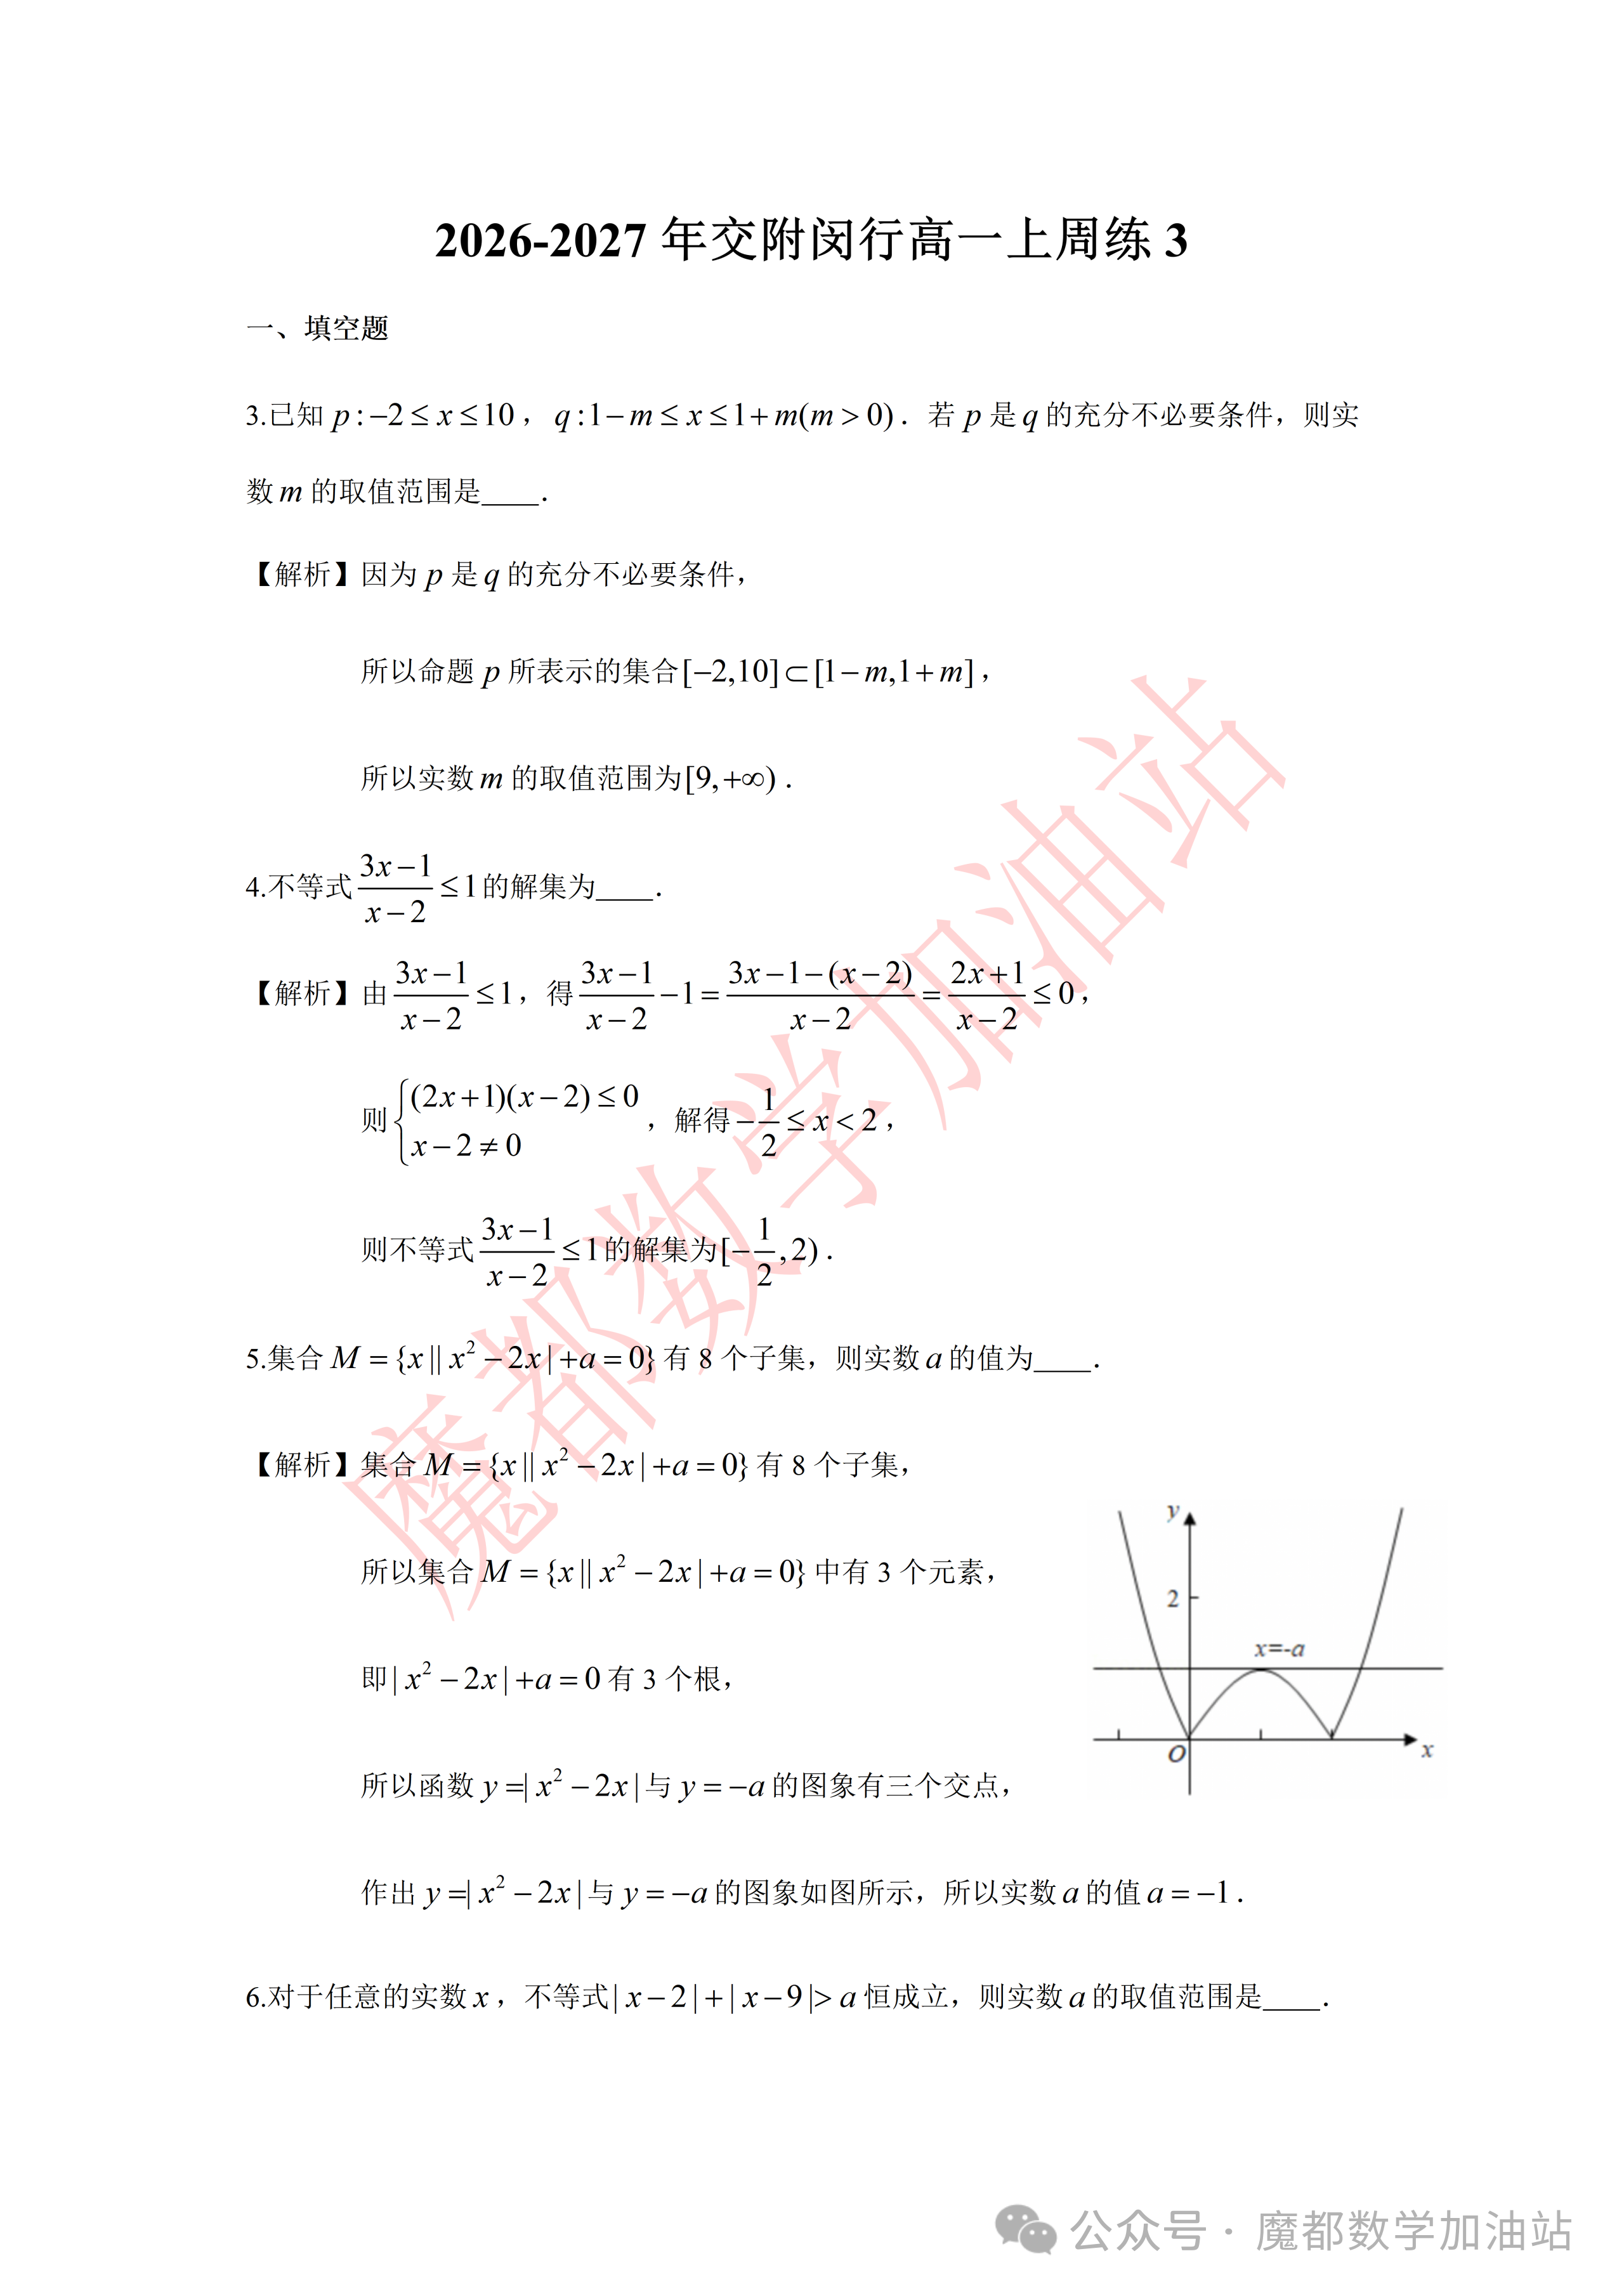
\includegraphics[width=0.14\textwidth,trim={1721bp 837bp 280bp 2297bp},clip]{../原图/高一43_交附闵行_周练3/01.png}
\end{center}

\solbegin
\step{集合 $M=\{x\mid |x^2-2x|+a=0\}$ 有 8 个子集，}
\step{所以集合 $M=\{x\mid |x^2-2x|+a=0\}$ 中有 3 个元素，}
\step{即 $|x^2-2x|+a=0$ 有 3 个根，}
\step{所以函数 $y=|x^2-2x|$ 与 $y=-a$ 的图象有三个交点，}
\step{作出 $y=|x^2-2x|$ 与 $y=-a$ 的图象如图所示，所以实数 $a$ 的值 $a=-1$.}
\solend

\fi

\item 对于任意的实数 $x$，不等式 $|x-2|+|x-9|>a$ 恒成立，则实数 $a$ 的取值范围是 \blankline[4.4em].

\ifanswer
\solbegin
\step{由绝对值的几何意义得 $|x-2|+|x-9|\geqslant7$，当且仅当 $2\leqslant x\leqslant9$ 时等号成立，}
\step{所以 $a<7$，}
\step{即 $a$ 的取值范围为 $(-\infty,7)$.}
\solend

\fi

\item 已知集合 $A=\{x\mid(a-1)x^2+3x-2=0\}$，$B=\{x\mid x^2-3x+2=0\}$，$A\subseteq B$，求实数 $a$ 的取值范围是 \blankline[4.4em].

\ifanswer
\solbegin
\step{由方程 $x^2-3x+2=0$，解得 $x=1$ 或 $x=2$，即 $B=\{1,2\}$，}
\step{因为 $A\subseteq B$，所以 $A=\varnothing$ 或 $A=\{1\}$ 或 $A=\{2\}$ 或 $A=\{1,2\}$，}
\step{当 $A=\varnothing$ 时，$a\neq1$，且 $\Delta=3^2-4(a-1)\times(-2)<0$，解得 $a<-\dfrac18$，}
\step{将 $x=1$ 代入方程 $(a-1)x^2+3x-2=0$，得 $a=0$，}
\step{此时 $A=\{x\mid-x^2+3x-2=0\}=\{1,2\}$，满足条件，}
\step{将 $x=2$ 代入方程 $(a-1)x^2+3x-2=0$，得到 $a=0$，上面已经验证满足条件，}
\step{综上所述，$a$ 的取值范围是 $\left(-\infty,-\dfrac18\right)\cup\{0\}$.}
\solend

\fi

\item 已知 $a$、$b$、$c$、$d$ 为常数，若不等式
$\dfrac{b}{x+a}+\dfrac{x+d}{x+c}<0$ 的解集为 $\left(-1,-\dfrac13\right)\cup\left(\dfrac12,1\right)$，
则不等式 $\dfrac{bx}{ax-1}+\dfrac{dx-1}{cx-1}<0$ 的解集为 \blankline[4.4em].

\ifanswer
\solbegin
\step{若 $x=0$，原不等式化为 $1<0$，不等式显然不成立，所以 $x\neq0$，}
\step{由 $\dfrac{bx}{ax-1}+\dfrac{dx-1}{cx-1}<0$，得 $\dfrac{b}{a-\dfrac1x}+\dfrac{d-\dfrac1x}{c-\dfrac1x}<0$，即 $\dfrac{b}{-\dfrac1x+a}+\dfrac{-\dfrac1x+d}{-\dfrac1x+c}<0$.}
\step{因为不等式 $\dfrac{b}{x+a}+\dfrac{x+d}{x+c}<0$ 的解集为 $\left(-1,-\dfrac13\right)\cup\left(\dfrac12,1\right)$，}
\step{所以 $-1<-\dfrac1x<-\dfrac13$ 或 $\dfrac12<-\dfrac1x<1$，解得 $1<x<3$ 或 $-2<x<-1$，}
\step{所以不等式 $\dfrac{bx}{ax-1}+\dfrac{dx-1}{cx-1}<0$ 的解集为 $(-2,-1)\cup(1,3)$.}
\solend

\fi

\item 正实数 $x$、$y$ 满足 $2x+3y-xy=0$，且存在这样的 $x$、$y$ 使不等式 $x+y<m+1$ 有解，则实数 $m$ 的取值范围是 \blankline[4.4em].

\ifanswer
\solbegin
\step{因为正实数 $x$、$y$ 满足 $2x+3y-xy=0$，则 $\dfrac2y+\dfrac3x=1$，$x>0$，$y>0$，}
\step{所以 $x+y=(x+y)\left(\dfrac3x+\dfrac2y\right)=3+\dfrac{2x}{y}+\dfrac{3y}{x}+2\geqslant2\sqrt{\dfrac{2x}{y}\times\dfrac{3y}{x}}+5=5+2\sqrt6$，}
\step{当且仅当 $\sqrt2x=\sqrt3y$ 时取等号，}
\step{存在这样的 $x$、$y$ 使不等式 $x+y<m+1$ 有解，则 $m+1>5+2\sqrt6$，}
\step{则 $m>4+2\sqrt6$，所以实数 $m$ 的取值范围是 $(4+2\sqrt6,+\infty)$.}
\solend

\fi

\item 若 $a$、$b$、$c\in\R$，$a^2+b^2+c^2=1$，则 $2ab+bc$ 的最大值为 \blankline[4.4em].

\ifanswer
\solbegin
\step{对于 $2ab+bc$，将 $b^2$ 拆分为 $\dfrac45b^2+\dfrac15b^2$，则 $a^2+\dfrac45b^2+c^2+\dfrac15b^2=1$，}
\step{$a^2+\dfrac45b^2\geqslant2\cdot a\cdot\dfrac2{\sqrt5}b=\dfrac4{\sqrt5}ab$，$c^2+\dfrac15b^2\geqslant2\cdot c\cdot\dfrac1{\sqrt5}b=\dfrac2{\sqrt5}bc$，}
\step{两式相加得 $1\geqslant\dfrac4{\sqrt5}ab+\dfrac2{\sqrt5}bc=\dfrac2{\sqrt5}(2ab+bc)$，故 $2ab+bc\leqslant\dfrac{\sqrt5}2$，}
\step{等号成立当且仅当 $a=\dfrac2{\sqrt5}b$，$c=\dfrac1{\sqrt5}b$，}
\step{代入 $a^2+b^2+c^2=1$，得 $\dfrac45b^2+b^2+\dfrac15b^2=2b^2=1$，即 $b=\dfrac{\sqrt2}2$，}
\step{此时 $a=\dfrac{\sqrt{10}}5$，$c=\dfrac{\sqrt{10}}{10}$，故 $2ab+bc$ 的最大值为 $\dfrac{\sqrt5}2$.}
\solend

\fi

\item 已知实数 $a$、$b$ 满足 $-3<a+2b<2$，$-1<2a-b<4$，则 $a+b$ 的取值范围为 \blankline[4.4em].

\ifanswer
\solbegin
\step{设 $a+b=m(a+2b)+n(2a-b)=(m+2n)a+(2m-n)b$，}
\step{所以 $\begin{cases}m+2n=1\\2m-n=1\end{cases}$，解得 $n=\dfrac15$，$m=\dfrac35$，所以 $a+b=\dfrac35(a+2b)+\dfrac15(2a-b)$，}
\step{因为 $-3<a+2b<2$，$-1<2a-b<4$，}
\step{所以 $-\dfrac95<\dfrac35(a+2b)<\dfrac65$，$-\dfrac15<\dfrac15(2a-b)<\dfrac45$，}
\step{相加得 $-2<\dfrac35(a+2b)+\dfrac15(2a-b)<2$，即 $-2<a+b<2$，}
\step{故 $a+b$ 的取值范围为 $(-2,2)$.}
\solend

\fi

% 注：原卷题干与解析均印作 \sqrt{2xyz}，但按其自身答案 8 与取等值（$y=\dfrac12$，
% $x=\dfrac{\sqrt3}4$，$z=\dfrac{\sqrt6}4$）代入只与 $\sqrt{2x^2y^2z^2}=\sqrt2\,xyz$ 相符，
% $\sqrt{2xyz}$ 与答案 8 不自洽，原卷如此，照录未改。
\item 已知正数 $x$、$y$、$z$ 满足 $2x^2+y^2+z^2=1$，则 $\dfrac{y+1}{\sqrt{2xyz}}$ 的最小值为 \blankline[4.4em].

\ifanswer
\solbegin
\step{由条件得 $2x^2+z^2=1-y^2=(1-y)(1+y)$，则 $1+y=\dfrac{2x^2+z^2}{1-y}$，}
\step{结合 $x$、$y$、$z>0$ 得原式 $=\dfrac{2x^2+z^2}{\sqrt{2xyz}(1-y)}\geqslant\dfrac{2\sqrt2xz}{\sqrt{2xyz}(1-y)}=\dfrac2{y(1-y)}$，}
\step{又 $y(1-y)\leqslant\left(\dfrac{y+1-y}2\right)^2=\dfrac14$，所以 $\dfrac2{y(1-y)}\geqslant\dfrac2{\frac14}=8$，}
\step{当且仅当 $\sqrt2x=z$，且 $y=1-y$，即 $y=\dfrac12$，$x=\dfrac{\sqrt3}4$，$z=\dfrac{\sqrt6}4$ 时取等号，}
\step{故 $\dfrac{y+1}{\sqrt{2xyz}}$ 最小值为 $8$.}
\solend

\fi

\end{enumerate}

\bigsec{二、选择题}

\begin{enumerate}
\setcounter{enumi}{12}

\item 已知关于 $x$ 的方程 $(1-k)x^2-2x-1=0$ 有实数根，则 $k$ 的取值范围是\mbox{（\quad）}

\keepwithprev
A. $k\leqslant2$ 且 $k\neq1$\qquad B. $k\leqslant2$\qquad
C. $k<2$ 且 $k\neq1$\qquad D. $k<2$

\ans{$A$}

\ifanswer
\solbegin
\step{由题意得 $\begin{cases}1-k\neq0\\\Delta=4+4(1-k)\geqslant0\end{cases}$，解不等式得 $\begin{cases}1\neq k\\2-k>0\end{cases}$，所以 $k\leqslant2$ 且 $k\neq1$，}
\step{故选 $A$.}
\solend

\fi

\item 不等式 $2|x+2|+|x-1|\geqslant5$ 成立的一个必要不充分条件是\mbox{（\quad）}

\keepwithprev
A. $x\leqslant-1$ 或 $x\geqslant0$\qquad B. $x\geqslant0$

C. $x\leqslant-\dfrac83$ 或 $x\geqslant0$\qquad D. $x\geqslant1$

\ans{$A$}

\ifanswer
\solbegin
\step{当 $x<-2$ 时，原不等式可化为 $-2x-4-x+1\geqslant5$，解得 $x\leqslant-\dfrac83$，}
\step{当 $-2\leqslant x<1$ 时，原不等式可化为 $2x+4-x+1\geqslant5$，解得 $0\leqslant x<1$，}
\step{当 $x\geqslant1$ 时，原不等式可化为 $2x+4+x-1\geqslant5$，解得 $x\geqslant\dfrac23$，得 $x\geqslant1$，}
\step{综上所述，不等式 $2|x+2|+|x-1|\geqslant5$ 成立的充要条件是 $x\leqslant-\dfrac83$ 或 $x\geqslant0$，}
\step{设 $A=\{x\mid x\leqslant-\dfrac83\text{ 或 }x\geqslant0\}$，}
\step{则不等式 $2|x+2|+|x-1|\geqslant5$ 成立的必要不充分条件，}
\step{其对应的集合 $B$ 满足 $A\subsetneq B$，对照各个选项，$A$ 项符合题意. 故选 $A$.}
\solend

\fi

\item 已知实数 $a>0$，$b>0$，$\dfrac1{a+1}+\dfrac1{b+1}=1$，则 $2a+3b$ 的最小值为\mbox{（\quad）}

\keepwithprev
A. $2\sqrt6$\qquad B. $3+2\sqrt6$\qquad
C. $5+2\sqrt6$\qquad D. $3+2\sqrt2$

\ans{$A$}

\ifanswer
\solbegin
\step{因为 $a>0$，$b>0$，$\dfrac1{a+1}+\dfrac1{b+1}=1$，}
\step{所以 $2a+3b=2(a+1)+3(b+1)-5=[2(a+1)+3(b+1)]\cdot\left(\dfrac1{a+1}+\dfrac1{b+1}\right)-5$}
\step{$=\left[2+3+\dfrac{3(b+1)}{a+1}+\dfrac{2(a+1)}{b+1}\right]-5\geqslant5+2\sqrt{\dfrac{3(b+1)}{a+1}\times\dfrac{2(a+1)}{b+1}}-5=2\sqrt6$，}
\step{当且仅当 $\dfrac{3(b+1)}{a+1}=\dfrac{2(a+1)}{b+1}$，即 $a=\dfrac{\sqrt6}2$，$b=\dfrac{\sqrt6}3$ 时取等号. 故选 $A$.}
\solend

\fi

\item 已知集合 $U=\{n\mid1\leqslant n\leqslant2027,\ n\in\N\}$，集合 $M\subseteq U$，若对于 $M$ 中任意两个不同的元素 $x$ 和 $y$，都有 $|x-y|>2$，则 $M$ 中元素个数的最大值是\mbox{（\quad）}

\keepwithprev
A. $676$\qquad B. $675$\qquad C. $672$\qquad D. $671$

\ans{$A$}

\ifanswer
\solbegin
\step{对于 $M$ 中的任意两个不同的元素 $x$、$y$，都有 $|x-y|>2$，}
\step{不妨设 $x>y$，都有 $x-y\geqslant3$，}
\step{要想 $M$ 所含元素个数最大，则要 $x-y$ 尽可能小，故需使得 $x-y$ 的最小值为 3，}
\step{将 $1\sim2027$ 这 2027 个元素按如下分组：}
\step{$\{1,2,3\}$，$\{4,5,6\}$，$\cdots$，$\{2023,2024,2025\}$，$\{2026,2027\}$，}
\step{故应在前 675 组中按周期 3 每组取一个元素，且第一组中不能取 3，}
\step{第一组中取 1 时，得 $M=\{1,4,7,\cdots,2023,2026\}$，}
\step{或 $M=\{1,4,7,\cdots,2023,2027\}$ 这样的集合，}
\step{第一组取 2 时，得 $M=\{2,5,8,\cdots,2024,2027\}$，}
\step{其中任意两元素差值 $x-y$（$x>y$）都大于 2，满足题意，}
\step{故 $M$ 所含元素个数的最大值为 $\dfrac{2025}{3}+1=676$. 故选 $A$.}
\solend

\fi

\end{enumerate}

\bigsec{三、解答题}

\begin{enumerate}
\setcounter{enumi}{16}

\item 已知 $a\in\R$，集合 $A=\left\{x\middle|\dfrac{2-x}{x+1}\leqslant0\right\}$，$B=\{x\mid x^2+(3-a)x-3a<0\}$.

\begin{enumerate}[label=(\arabic*)]
\item 当 $a=\dfrac13$ 时，求 $A$ 和 $B$；
\item 已知 $A\cup B=A$，求实数 $a$ 的取值范围.
\end{enumerate}

\ifanswer
\solbegin
\stepm{(1)}{由 $\dfrac{2-x}{x+1}\leqslant0$，得 $\begin{cases}(2-x)(x+1)\leqslant0\\x\neq-1\end{cases}$，解得 $x<-1$ 或 $x\geqslant2$，}
\step{则 $A=\{x\mid x<-1\text{ 或 }x\geqslant2\}$；}
\step{$B=\{x\mid x^2+(3-a)x-3a<0\}=\{x\mid(x+3)(x-a)<0\}$，}
% 注：原卷此行印作 $(x+2)\left(x-\dfrac13\right)$，按前一行 $B=\{x\mid(x+3)(x-a)<0\}$ 应为
% $(x+3)\left(x-\dfrac13\right)$，原卷如此，照录未改。
\step{当 $a=\dfrac13$ 时，$B=\left\{x\middle|(x+2)\left(x-\dfrac13\right)<0\right\}$，}
\step{解得 $B=\left\{x\middle|-3<x<\dfrac13\right\}$.}
\stepm{(2)}{由 $A\cup B=A$，得 $B\subseteq A$，}
\step{①当 $B=\varnothing$ 时，得 $a=-3$，符合题意；}
\step{②当 $B\neq\varnothing$ 时，若 $a>-3$，则 $B=\{x\mid-3<x<a\}$，}
\step{由 $B\subseteq A$，得 $a\leqslant-1$，此时 $-3<a\leqslant-1$；}
\step{若 $a<-3$，则 $B=\{x\mid a<x<-3\}$，此时 $B\subseteq A$ 恒成立，}
\step{故 $a<-3$ 符合题意；}
\step{综上所述，实数 $a$ 的取值范围为 $a\leqslant-1$.}
\solend

\fi

\ansspace[6]

\item 甲乙两地的高速公路全长 166 千米，汽车从甲地进入该高速公路后匀速行驶到乙地，车速 $v\in[70,120]$（千米/时）. 已知汽车每小时的运输成本（以元为单位）由可变部分和固定部分组成：可变部分为 $0.02v^2$，固定部分为 220 元.

\begin{enumerate}[label=(\arabic*)]
\item 若每小时的运输成本不高于 420 元，汽车的速度应该控制在什么范围？
\item 汽车应以多大速度行驶才能使全程运输成本最小？最小运输成本约为多少元？（结果保留整数）
\end{enumerate}

\ifanswer
\solbegin
\stepm{(1)}{已知汽车每小时的运输成本（以元为单位）由可变部分和固定部分组成：}
\step{可变部分为 $0.02v^2$，固定部分为 220 元，}
\step{则汽车每小时的运输成本为 $0.02v^2+220$（元），}
\step{若每小时的运输成本不高于 420 元，}
\step{则 $0.02v^2+220\leqslant420$，解得 $v^2\leqslant10000$，}
\step{得 $70\leqslant v\leqslant100$，即 $v\in[70,100]$（千米/时），}
\step{则此时汽车的速度 $v$ 应该控制在 $[70,100]$（千米/时）；}
\stepm{(2)}{因为汽车从甲地进入该高速公路后匀速行驶到乙地，}
\step{车速 $v\in[70,120]$（千米/时），所以汽车的行驶时间为 $\dfrac{166}{v}$（小时），}
\step{所以全程运输成本 $y=\dfrac{166}{v}(0.02v^2+220)=3.32v+\dfrac{36520}{v}$，}
% 注：原卷此行印作 $v\in[70,100]$，与题干的 $v\in[70,120]$ 不自洽（若 $v\in[70,100]$，
% 最小值应在 $v=100$ 处取得，与下文 $v=10\sqrt{110}\approx105$ 矛盾），原卷如此，照录未改。
\step{$v\in[70,100]$，}
\step{由基本不等式得 $y=3.32v+\dfrac{36520}{v}\geqslant2\sqrt{3.32v\times\dfrac{36520}{v}}\approx696$，}
\step{当且仅当 $3.32v=\dfrac{36520}{v}$，即 $v=10\sqrt{110}\approx105$ 时取等号，}
\step{汽车应以 105（千米/时）行驶才能使全程运输成本最小，}
\step{最小运输成本约为 696 元.}
\solend

\fi

\ansspace[8]

\item
\begin{enumerate}[label=(\arabic*)]
\item 已知 $a$、$b$、$c$ 为实数，求证：$|a-b|\leqslant|a-c|+|b-c|$，并说明等号成立的条件；
\item 设 $x\in\R$，求方程 $|3x-8|=|5-x|+|2x-3|$ 的解集.
\end{enumerate}

\ifanswer
% 注：原卷第 19 题未印【解析】，仅印一行【答案】"（1）(a-c)(b-c)≤0；
% （2）(-∞,3/2]∪[5,+∞)"。(1) 的两行推导为本稿所补，(2) 照录原卷答案。
% 又题干作"方程"，而所给答案 (-∞,3/2]∪[5,+∞) 实为不等式 |3x-8|≤|5-x|+|2x-3| 的解集，
% 与"方程"不合，原卷如此，照录未改。
\solbegin
\stepm{(1)}{由三角不等式 $|a-b|=|(a-c)-(b-c)|\leqslant|a-c|+|b-c|$，}
\step{当且仅当 $(a-c)(b-c)\leqslant0$ 时等号成立.}
\stepm{(2)}{$\left(-\infty,\dfrac32\right]\cup[5,+\infty)$.}
\solend

\fi

\ansspace[6]

\item 已知正实数 $a$、$b$ 满足 $a+b=1$，求 $\dfrac1a+\dfrac1b$ 的最小值. 其中一种解法是：

\[
\begin{aligned}
\dfrac1a+\dfrac1b
&=\left(\dfrac1a+\dfrac1b\right)(a+b)\\
&=1+\dfrac ba+\dfrac ab+1\\
&\geqslant2+2\sqrt{\dfrac ba\times\dfrac ab}=2+2=4.
\end{aligned}
\]
当且仅当 $\dfrac ba=\dfrac ab$ 且 $a+b=1$ 时即 $a=b=\dfrac12$ 时取等号.
学习上述解法并解决下列问题：

\begin{enumerate}[label=(\arabic*)]
\item 若正实数 $x$、$y$ 满足 $x+y=xy$，求 $2x+y$ 的最小值；
\item 若实数 $a$、$b$、$x$、$y$ 满足 $\dfrac{x^2}{a^2}+\dfrac{y^2}{b^2}=1$，求证：$a^2+b^2\geqslant(x+y)^2$；
\item 求代数式 $M=\sqrt{m-1}+\sqrt{3-m}$ 的最大值，并求出使得 $M$ 最大的 $m$ 的值.
\end{enumerate}

\ifanswer
\solbegin
\stepm{(1)}{因为正实数 $x$、$y$ 满足 $x+y=xy$，$\dfrac{x+y}{xy}=1\Rightarrow\dfrac1y+\dfrac1x=1$，}
\step{所以 $(2x+y)\times1=(2x+y)\left(\dfrac1y+\dfrac1x\right)=3+\dfrac{2x}{y}+\dfrac yx\geqslant3+2\sqrt{\dfrac{2x}{y}\cdot\dfrac yx}=3+2\sqrt2$，}
\step{当且仅当 $\dfrac{2x}{y}=\dfrac yx$ 且 $\dfrac1y+\dfrac1x=1$ 时取等号，}
\step{解得 $x=\dfrac{2+\sqrt2}2$，$y=\sqrt2x=\sqrt2\times\dfrac{2+\sqrt2}2=1+\sqrt2$，}
\step{所以 $2x+y$ 的最小值为 $3+2\sqrt2$；}
\stepm{(2)}{因为 $\dfrac{x^2}{a^2}+\dfrac{y^2}{b^2}=1$，}
\step{所以 $a^2+b^2=(a^2+b^2)\left(\dfrac{x^2}{a^2}+\dfrac{y^2}{b^2}\right)=x^2+y^2+\dfrac{b^2x^2}{a^2}+\dfrac{a^2y^2}{b^2}$，}
\step{因为 $\dfrac{b^2x^2}{a^2}+\dfrac{a^2y^2}{b^2}\geqslant2\sqrt{\dfrac{b^2x^2}{a^2}\times\dfrac{a^2y^2}{b^2}}=2\sqrt{x^2y^2}=2|xy|$，}
\step{当且仅当 $\dfrac{b^2x^2}{a^2}=\dfrac{a^2y^2}{b^2}$ 时取等号，}
\step{所以 $x^2+y^2+\dfrac{b^2x^2}{a^2}+\dfrac{a^2y^2}{b^2}\geqslant x^2+y^2+2|xy|\geqslant x^2+y^2+2xy=(x+y)^2$，}
\step{所以 $a^2+b^2\geqslant(x+y)^2$；}
\stepm{(3)}{因为 $M=\sqrt{m-1}+\sqrt{3-m}$，所以 $\begin{cases}m-1\geqslant0\\3-m\geqslant0\end{cases}$，解得 $1\leqslant m\leqslant3$，}
\step{所以 $M^2=(\sqrt{m-1}+\sqrt{3-m})^2=2+2\sqrt{(3-m)(m-1)}$，}
\step{由基本不等式得 $(3-m)(m-1)\leqslant\left(\dfrac{(3-m)+(m-1)}2\right)^2=1$，}
\step{当且仅当 $3-m=m-1$ 时取等号，解得 $m=2$，}
\step{所以 $M^2=2+2\sqrt{(3-m)(m-1)}\leqslant2+2\sqrt1=4$，}
\step{因为 $M>0$，所以 $M\leqslant2$，所以 $M$ 最大值为 2，此时 $m$ 的值为 2.}
\solend

\fi

\ansspace[8]

\item 若有限个正整数组成的集合 $A$ 中至少有两个元素，且对于任意的 $x,y\in A$（$x>y$），都有 $\dfrac{y^2}{x-y}\in A$，则称 $A$ 为“L-集合”.

\begin{enumerate}[label=(\arabic*)]
\item 判断 $\{1,2,4\}$ 是否为“L-集合”，说明理由；
\item 若双元素集 $M$ 为“L-集合”，且 $4\in M$，求所有满足条件的集合 $M$；
\item 求所有满足条件的“L-集合”.
\end{enumerate}

\ifanswer
\solbegin
\stepm{(1)}{若至少由两个元素构成的有限集合 $A\subseteq\N^*$，}
% 注：原卷下一行"都有"后未印分数 \dfrac{y^2}{x-y}，径作"都有 A"，原卷如此，照录未改。
\step{且对于任意的 $x$、$y\in A$（$x>y$），都有 $A$，则称 $A$ 为“L-集合”，}
\step{$\{1,2,4\}$ 不为“L-集合”，理由如下：}
\step{因为 $\dfrac{1^2}{4-1}=\dfrac13\notin\{1,2,4\}$，所以 $\{1,2,4\}$ 不是“L-集合”.}
\stepm{(2)}{设 $M=\{4,m\}$（$m\in\N^*$，$m\neq4$），}
\step{若 $m<4$，则 $\dfrac{m^2}{4-m}=m$ 或 $\dfrac{m^2}{4-m}=4$，}
\step{由 $\dfrac{m^2}{4-m}=m$，解得 $m=2$，$m=0$（舍去），此时 $M=\{2,4\}$；}
\step{由 $\dfrac{m^2}{4-m}=4$ 化为 $m^2+4m-16=0$，而 $\Delta=4^2+4\times16=80$，}
\step{故方程无正整数解.}
\step{若 $m>4$，则 $\dfrac{4^2}{m-4}=4$ 或 $\dfrac{4^2}{m-4}=m$，}
\step{由 $\dfrac{4^2}{m-4}=4$，解得 $m=8$，此时 $M=\{4,8\}$；}
\step{由 $\dfrac{4^2}{m-4}=m$ 化为 $m^2-4m-16=0$，而 $\Delta=4^2+4\times16=80$，}
\step{故方程无正整数解.}
\step{综上，双元素集 $M$ 为“L-集合”，且 $4\in M$，}
\step{则所有满足条件的集合 $M$ 为 $\{4,8\}$，$\{2,4\}$.}
\stepm{(3)}{若“L-集合”为双元素集，}
\step{不妨设 $M=\{k,m\}$（$k,m\in\N^*$，$m>k$），则 $\dfrac{k^2}{m-k}=k$ 或 $\dfrac{k^2}{m-k}=m$，}
\step{由 $\dfrac{k^2}{m-k}=k$，则 $2k^2=mk$，而 $m>k$，故 $m=2k$，此时 $M=\{k,2k\}$；}
\step{由 $\dfrac{k^2}{m-k}=m$，则 $m^2-mk-k^2=0$，而 $\Delta=5k^2$，显然不存在正整数解；}
\step{所以，“L-集合”为 $\{k,2k\}$，其中 $k\in\N^*$.}
\step{若“L-集合”含有两个以上的元素，}
\step{设最小的元素为 $b$，最大的元素为 $a$，第二大的元素为 $n$，}
\step{则 $\dfrac{b^2}{a-b}$，$\dfrac{n^2}{a-n}$ 是“L-集合”中的元素，}
% 注：原卷下一行未印"由于'L-集合'中的元素均为正整数"一语，径作"若 \dfrac{b^2}{a-b}\geqslant b"，
% 原卷如此，照录未改。
\step{若 $\dfrac{b^2}{a-b}\geqslant b$，解得 $a\leqslant2b$，}
\step{若 $\dfrac{n^2}{a-n}\leqslant n$，则 $a\geqslant2n>2b$，矛盾，}
\step{若 $\dfrac{n^2}{a-n}=a$，该方程的解为 $n=\dfrac{\sqrt5-1}2a$，则 $n$、$a$ 不可能同时为整数，}
\step{无解.}
\step{所以所有满足条件的“L-集合”为 $\{k,2k\}$，其中 $k\in\N^*$.}
\solend

\fi

\ansspace*[10]

\end{enumerate}

\end{document}
"
% 紧凑版：xelatex "\def\iscompact{1}% 高一43_交附闵行_周练3.tex
%   —— 高一上数学“2026-2027 年交附闵行高一上周练3”（试卷版/答案版）
% 试卷版：xelatex 高一43_交附闵行_周练3.tex
% 答案版：xelatex "\def\isanswer{1}\input{高一43_交附闵行_周练3.tex}"
% 紧凑版：xelatex "\def\iscompact{1}\input{高一43_交附闵行_周练3.tex}"
%
% 原始材料是微信公众号图文（公众号“魔都数学加油站”，作者破晓，2026-10-01 21:37，
% 原文标题“27学年高一43——2026-2027年上海市交附闵行高一上周练3”，
% https://mp.weixin.qq.com/s/-rgkOD9jJVpug6s0uSbwmQ）。正文为 12 张 PNG 页；
% 第 01、05、09、12 页 2560×3620，其余第 02—04、06—08、10—11 页 4762×6735。
% 原文本身是讲评版，题目下方印有解析/答案；题目与讲解照原卷转录，保留原卷错误。
%
% 卷首标题：原卷印作“2026-2027 年交附闵行高一上周练3”，公众号标题中的“上海市”
% 三字不在卷面标题中，本稿依卷面录入；年份区间按全稿惯例排 en dash。
%
% 与原卷的排版差异：
%   ① 原文从第 3 题开始（第 1、2 题未在这篇推文中发布），本稿保留原题号 3—21；
%   ② 原卷本就印有“一、填空题”“二、选择题”“三、解答题”，本稿照原卷分节，
%      改排为全稿统一的大节标题；
%   ③ 原卷未印副标题，本稿按“知识模块”口径补出“集合与常用逻辑用语、不等式”；
%   ④ 原卷填空横线依全稿惯例排为 \blankline[4.4em]；选择题答案只在答案版以 \ans{} 显示，
%      解答区以 \ifanswer 分离；解答题按原卷留出标准作答空间；
%   ⑤ 第 5 题图取自原卷第 1 页截图并裁入本稿，不另建图档；公众号水印不录入。
%      原卷图页分页不保留，正文依本稿版心重新分页。
%
% 原卷存疑/错误（均照录，未改）：
%   ① 第 9 题原卷题干即作"正实数 x、y"，与解析 x>0、y>0 相容，并无矛盾（初稿曾误记
%      题干只称"实数"并据此指原卷不自洽，2026-10-05 回原图核对订正）。
%   ② 第 11 题解析"相加得"一行原卷印作 -2<3/5(a+2b)+1/5(2a-b)<2，第一项系数 3/5
%      原卷不缺（初稿漏抄致该行按字面不成立，2026-10-05 已按原卷补回）。
%   ③ 第 13 题答案印 A，解析以“1-k≠0”排除 k=1；但 k=1 时原方程为 -2x-1=0，
%      仍有实数根，按题意应选 B。本稿保留原卷答案 A 及其解析，不代为订正。
%
\documentclass[a4paper,11pt]{article}
\usepackage{common}
\usepackage{graphicx}

\begin{document}

\examtitlest[3]{2026--2027 年交附闵行高一上周练 3}{集合与常用逻辑用语、不等式}

\bigsec{一、填空题}

\begin{enumerate}
\setcounter{enumi}{2}

\item 已知 $p\colon -2\leqslant x\leqslant10$，$q\colon 1-m\leqslant x\leqslant1+m$（$m>0$）. 若 $p$ 是 $q$ 的充分不必要条件，则实数 $m$ 的取值范围是 \blankline[4.4em].

\ifanswer
\solbegin
\step{因为 $p$ 是 $q$ 的充分不必要条件，}
\step{所以命题 $p$ 所表示的集合 $[-2,10]\subset[1-m,1+m]$，}
\step{所以实数 $m$ 的取值范围为 $[9,+\infty)$.}
\solend

\fi

\item 不等式 $\dfrac{3x-1}{x-2}\leqslant1$ 的解集为 \blankline[4.4em].

\ifanswer
\solbegin
\step{由 $\dfrac{3x-1}{x-2}-1=\dfrac{3x-1-(x-2)}{x-2}=\dfrac{2x+1}{x-2}\leqslant0$，}
\step{则 $\begin{cases}(2x+1)(x-2)\leqslant0\\x-2\neq0\end{cases}$，解得 $-\dfrac12\leqslant x<2$，}
\step{则不等式 $\dfrac{3x-1}{x-2}\leqslant1$ 的解集为 $\left[-\dfrac12,2\right)$.}
\solend

\fi

\item 集合 $M=\{x\mid |x^2-2x|+a=0\}$ 有 8 个子集，则实数 $a$ 的值为 \blankline[4.4em].

\ifanswer
\begin{center}
% 图取自原卷第 1 页；用原图裁切，未重绘。
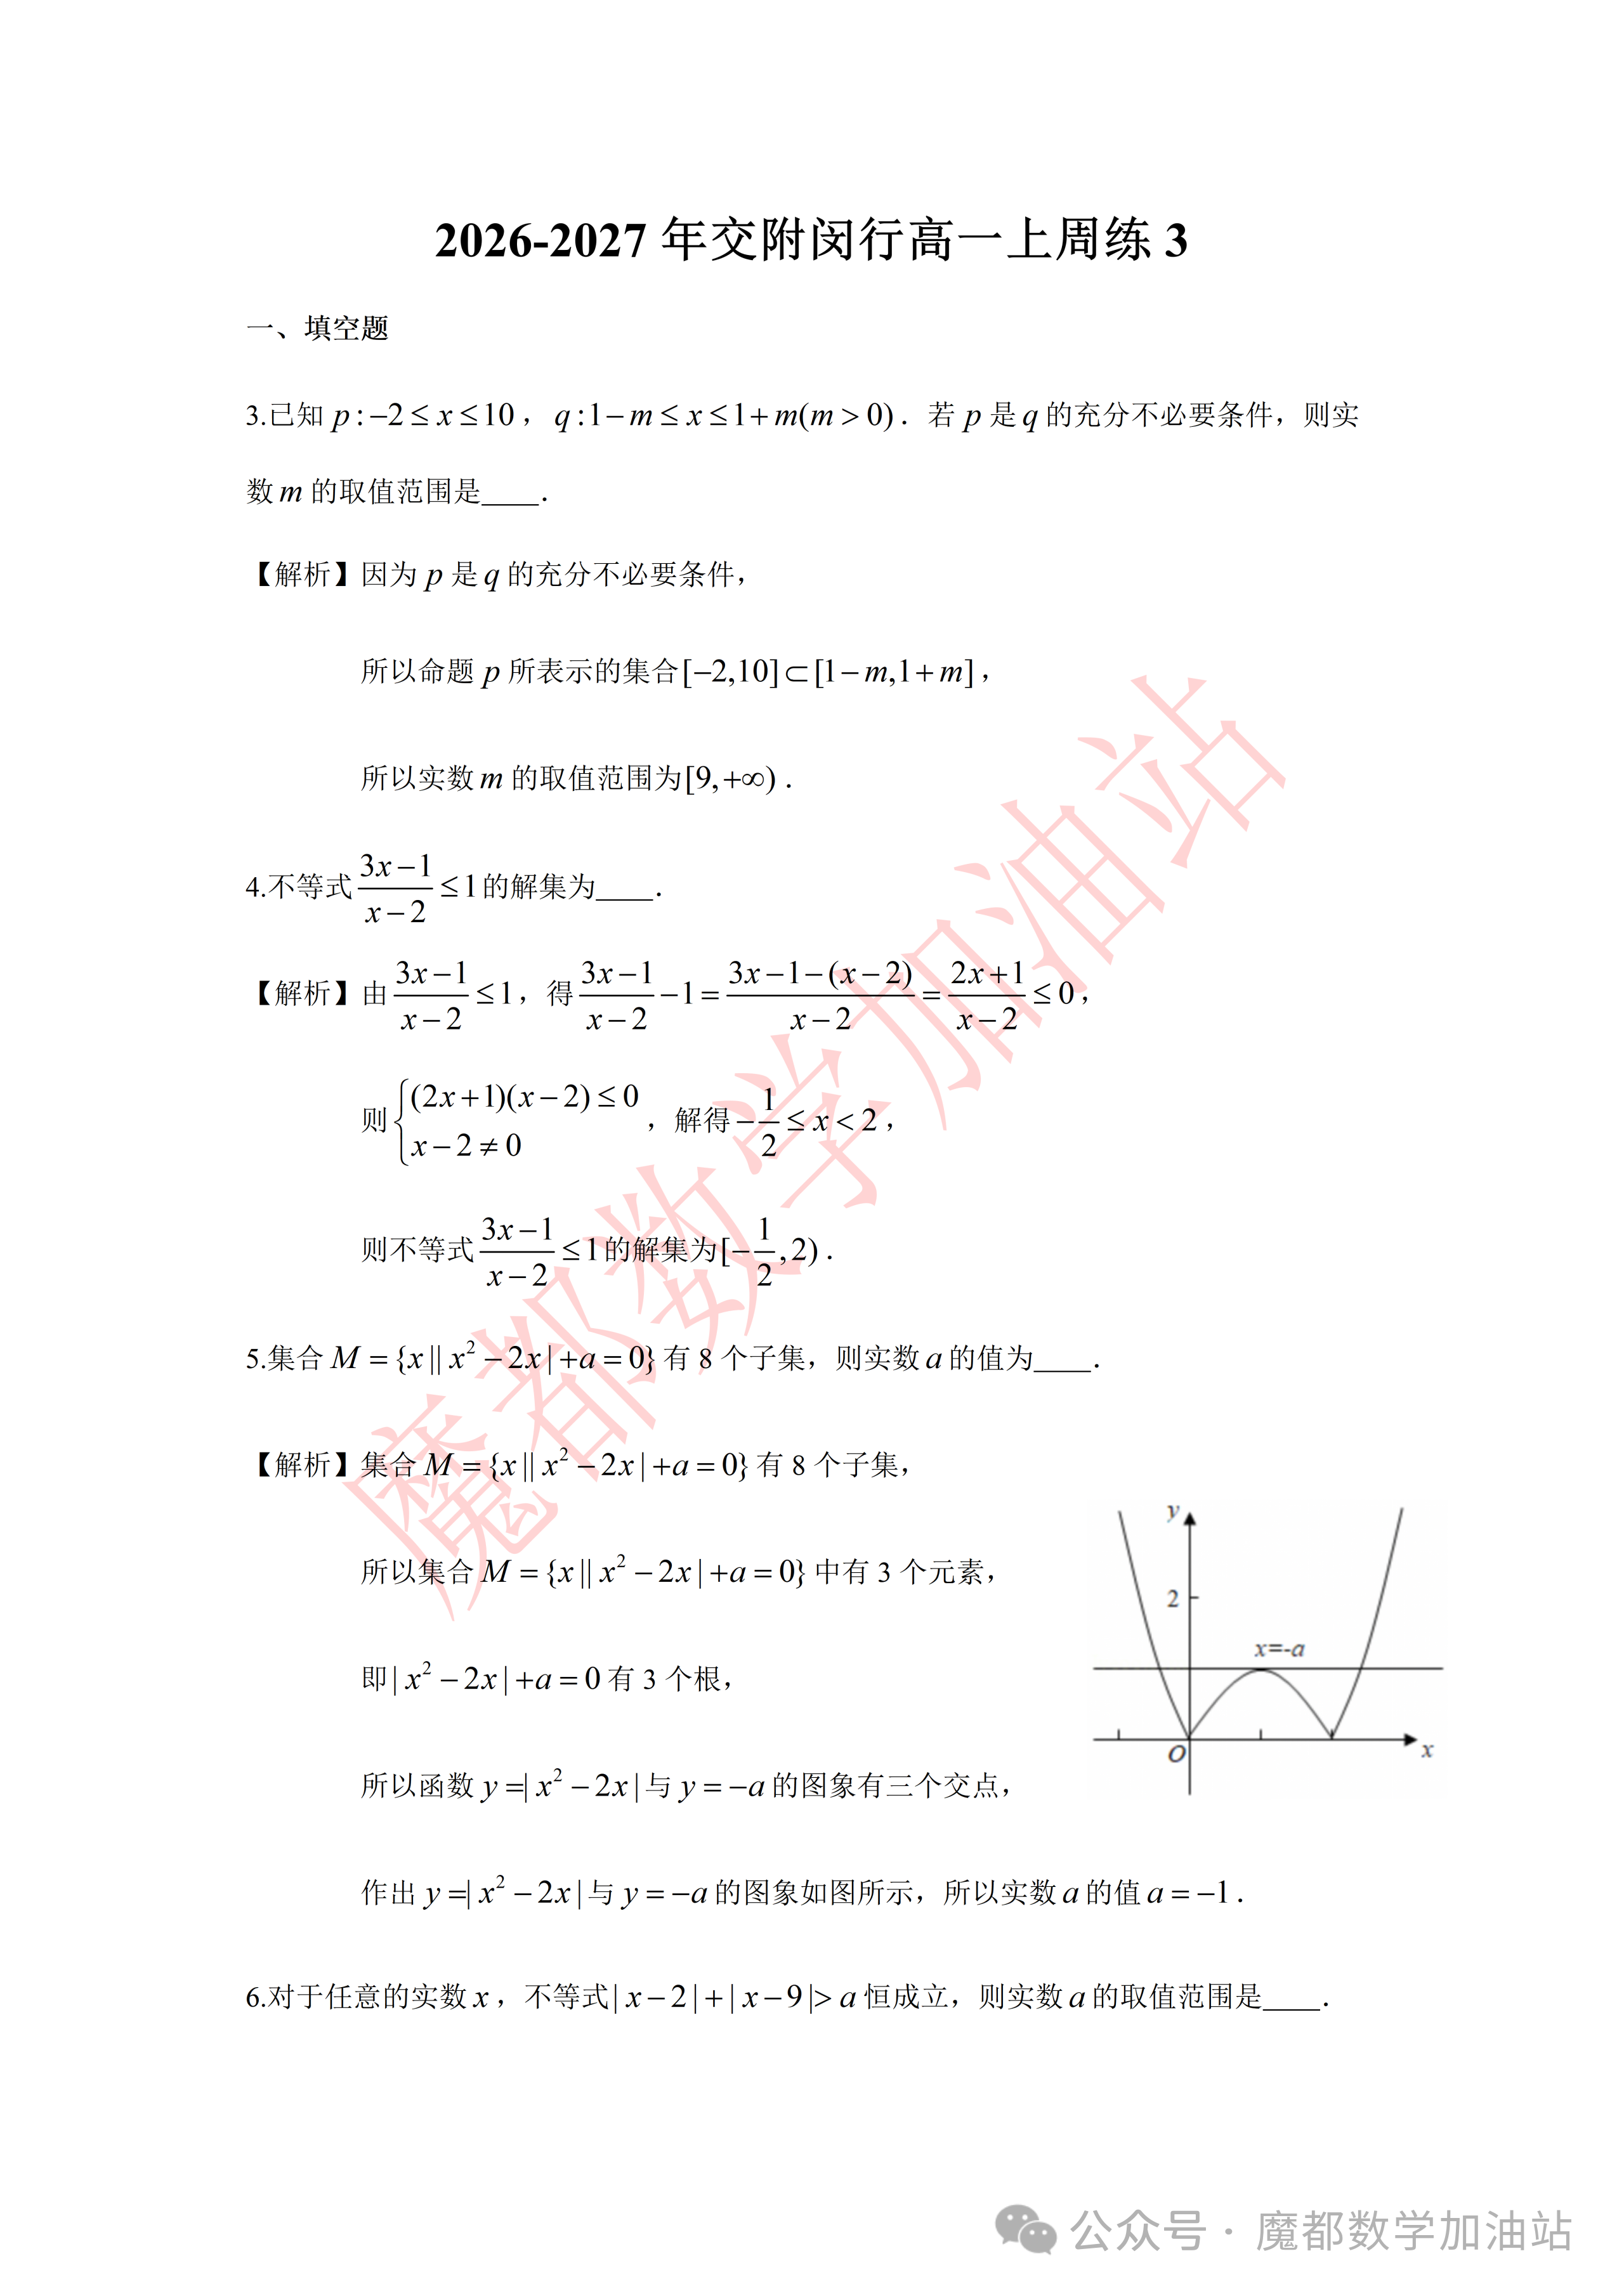
\includegraphics[width=0.14\textwidth,trim={1721bp 837bp 280bp 2297bp},clip]{../原图/高一43_交附闵行_周练3/01.png}
\end{center}

\solbegin
\step{集合 $M=\{x\mid |x^2-2x|+a=0\}$ 有 8 个子集，}
\step{所以集合 $M=\{x\mid |x^2-2x|+a=0\}$ 中有 3 个元素，}
\step{即 $|x^2-2x|+a=0$ 有 3 个根，}
\step{所以函数 $y=|x^2-2x|$ 与 $y=-a$ 的图象有三个交点，}
\step{作出 $y=|x^2-2x|$ 与 $y=-a$ 的图象如图所示，所以实数 $a$ 的值 $a=-1$.}
\solend

\fi

\item 对于任意的实数 $x$，不等式 $|x-2|+|x-9|>a$ 恒成立，则实数 $a$ 的取值范围是 \blankline[4.4em].

\ifanswer
\solbegin
\step{由绝对值的几何意义得 $|x-2|+|x-9|\geqslant7$，当且仅当 $2\leqslant x\leqslant9$ 时等号成立，}
\step{所以 $a<7$，}
\step{即 $a$ 的取值范围为 $(-\infty,7)$.}
\solend

\fi

\item 已知集合 $A=\{x\mid(a-1)x^2+3x-2=0\}$，$B=\{x\mid x^2-3x+2=0\}$，$A\subseteq B$，求实数 $a$ 的取值范围是 \blankline[4.4em].

\ifanswer
\solbegin
\step{由方程 $x^2-3x+2=0$，解得 $x=1$ 或 $x=2$，即 $B=\{1,2\}$，}
\step{因为 $A\subseteq B$，所以 $A=\varnothing$ 或 $A=\{1\}$ 或 $A=\{2\}$ 或 $A=\{1,2\}$，}
\step{当 $A=\varnothing$ 时，$a\neq1$，且 $\Delta=3^2-4(a-1)\times(-2)<0$，解得 $a<-\dfrac18$，}
\step{将 $x=1$ 代入方程 $(a-1)x^2+3x-2=0$，得 $a=0$，}
\step{此时 $A=\{x\mid-x^2+3x-2=0\}=\{1,2\}$，满足条件，}
\step{将 $x=2$ 代入方程 $(a-1)x^2+3x-2=0$，得到 $a=0$，上面已经验证满足条件，}
\step{综上所述，$a$ 的取值范围是 $\left(-\infty,-\dfrac18\right)\cup\{0\}$.}
\solend

\fi

\item 已知 $a$、$b$、$c$、$d$ 为常数，若不等式
$\dfrac{b}{x+a}+\dfrac{x+d}{x+c}<0$ 的解集为 $\left(-1,-\dfrac13\right)\cup\left(\dfrac12,1\right)$，
则不等式 $\dfrac{bx}{ax-1}+\dfrac{dx-1}{cx-1}<0$ 的解集为 \blankline[4.4em].

\ifanswer
\solbegin
\step{若 $x=0$，原不等式化为 $1<0$，不等式显然不成立，所以 $x\neq0$，}
\step{由 $\dfrac{bx}{ax-1}+\dfrac{dx-1}{cx-1}<0$，得 $\dfrac{b}{a-\dfrac1x}+\dfrac{d-\dfrac1x}{c-\dfrac1x}<0$，即 $\dfrac{b}{-\dfrac1x+a}+\dfrac{-\dfrac1x+d}{-\dfrac1x+c}<0$.}
\step{因为不等式 $\dfrac{b}{x+a}+\dfrac{x+d}{x+c}<0$ 的解集为 $\left(-1,-\dfrac13\right)\cup\left(\dfrac12,1\right)$，}
\step{所以 $-1<-\dfrac1x<-\dfrac13$ 或 $\dfrac12<-\dfrac1x<1$，解得 $1<x<3$ 或 $-2<x<-1$，}
\step{所以不等式 $\dfrac{bx}{ax-1}+\dfrac{dx-1}{cx-1}<0$ 的解集为 $(-2,-1)\cup(1,3)$.}
\solend

\fi

\item 正实数 $x$、$y$ 满足 $2x+3y-xy=0$，且存在这样的 $x$、$y$ 使不等式 $x+y<m+1$ 有解，则实数 $m$ 的取值范围是 \blankline[4.4em].

\ifanswer
\solbegin
\step{因为正实数 $x$、$y$ 满足 $2x+3y-xy=0$，则 $\dfrac2y+\dfrac3x=1$，$x>0$，$y>0$，}
\step{所以 $x+y=(x+y)\left(\dfrac3x+\dfrac2y\right)=3+\dfrac{2x}{y}+\dfrac{3y}{x}+2\geqslant2\sqrt{\dfrac{2x}{y}\times\dfrac{3y}{x}}+5=5+2\sqrt6$，}
\step{当且仅当 $\sqrt2x=\sqrt3y$ 时取等号，}
\step{存在这样的 $x$、$y$ 使不等式 $x+y<m+1$ 有解，则 $m+1>5+2\sqrt6$，}
\step{则 $m>4+2\sqrt6$，所以实数 $m$ 的取值范围是 $(4+2\sqrt6,+\infty)$.}
\solend

\fi

\item 若 $a$、$b$、$c\in\R$，$a^2+b^2+c^2=1$，则 $2ab+bc$ 的最大值为 \blankline[4.4em].

\ifanswer
\solbegin
\step{对于 $2ab+bc$，将 $b^2$ 拆分为 $\dfrac45b^2+\dfrac15b^2$，则 $a^2+\dfrac45b^2+c^2+\dfrac15b^2=1$，}
\step{$a^2+\dfrac45b^2\geqslant2\cdot a\cdot\dfrac2{\sqrt5}b=\dfrac4{\sqrt5}ab$，$c^2+\dfrac15b^2\geqslant2\cdot c\cdot\dfrac1{\sqrt5}b=\dfrac2{\sqrt5}bc$，}
\step{两式相加得 $1\geqslant\dfrac4{\sqrt5}ab+\dfrac2{\sqrt5}bc=\dfrac2{\sqrt5}(2ab+bc)$，故 $2ab+bc\leqslant\dfrac{\sqrt5}2$，}
\step{等号成立当且仅当 $a=\dfrac2{\sqrt5}b$，$c=\dfrac1{\sqrt5}b$，}
\step{代入 $a^2+b^2+c^2=1$，得 $\dfrac45b^2+b^2+\dfrac15b^2=2b^2=1$，即 $b=\dfrac{\sqrt2}2$，}
\step{此时 $a=\dfrac{\sqrt{10}}5$，$c=\dfrac{\sqrt{10}}{10}$，故 $2ab+bc$ 的最大值为 $\dfrac{\sqrt5}2$.}
\solend

\fi

\item 已知实数 $a$、$b$ 满足 $-3<a+2b<2$，$-1<2a-b<4$，则 $a+b$ 的取值范围为 \blankline[4.4em].

\ifanswer
\solbegin
\step{设 $a+b=m(a+2b)+n(2a-b)=(m+2n)a+(2m-n)b$，}
\step{所以 $\begin{cases}m+2n=1\\2m-n=1\end{cases}$，解得 $n=\dfrac15$，$m=\dfrac35$，所以 $a+b=\dfrac35(a+2b)+\dfrac15(2a-b)$，}
\step{因为 $-3<a+2b<2$，$-1<2a-b<4$，}
\step{所以 $-\dfrac95<\dfrac35(a+2b)<\dfrac65$，$-\dfrac15<\dfrac15(2a-b)<\dfrac45$，}
\step{相加得 $-2<\dfrac35(a+2b)+\dfrac15(2a-b)<2$，即 $-2<a+b<2$，}
\step{故 $a+b$ 的取值范围为 $(-2,2)$.}
\solend

\fi

% 注：原卷题干与解析均印作 \sqrt{2xyz}，但按其自身答案 8 与取等值（$y=\dfrac12$，
% $x=\dfrac{\sqrt3}4$，$z=\dfrac{\sqrt6}4$）代入只与 $\sqrt{2x^2y^2z^2}=\sqrt2\,xyz$ 相符，
% $\sqrt{2xyz}$ 与答案 8 不自洽，原卷如此，照录未改。
\item 已知正数 $x$、$y$、$z$ 满足 $2x^2+y^2+z^2=1$，则 $\dfrac{y+1}{\sqrt{2xyz}}$ 的最小值为 \blankline[4.4em].

\ifanswer
\solbegin
\step{由条件得 $2x^2+z^2=1-y^2=(1-y)(1+y)$，则 $1+y=\dfrac{2x^2+z^2}{1-y}$，}
\step{结合 $x$、$y$、$z>0$ 得原式 $=\dfrac{2x^2+z^2}{\sqrt{2xyz}(1-y)}\geqslant\dfrac{2\sqrt2xz}{\sqrt{2xyz}(1-y)}=\dfrac2{y(1-y)}$，}
\step{又 $y(1-y)\leqslant\left(\dfrac{y+1-y}2\right)^2=\dfrac14$，所以 $\dfrac2{y(1-y)}\geqslant\dfrac2{\frac14}=8$，}
\step{当且仅当 $\sqrt2x=z$，且 $y=1-y$，即 $y=\dfrac12$，$x=\dfrac{\sqrt3}4$，$z=\dfrac{\sqrt6}4$ 时取等号，}
\step{故 $\dfrac{y+1}{\sqrt{2xyz}}$ 最小值为 $8$.}
\solend

\fi

\end{enumerate}

\bigsec{二、选择题}

\begin{enumerate}
\setcounter{enumi}{12}

\item 已知关于 $x$ 的方程 $(1-k)x^2-2x-1=0$ 有实数根，则 $k$ 的取值范围是\mbox{（\quad）}

\keepwithprev
A. $k\leqslant2$ 且 $k\neq1$\qquad B. $k\leqslant2$\qquad
C. $k<2$ 且 $k\neq1$\qquad D. $k<2$

\ans{$A$}

\ifanswer
\solbegin
\step{由题意得 $\begin{cases}1-k\neq0\\\Delta=4+4(1-k)\geqslant0\end{cases}$，解不等式得 $\begin{cases}1\neq k\\2-k>0\end{cases}$，所以 $k\leqslant2$ 且 $k\neq1$，}
\step{故选 $A$.}
\solend

\fi

\item 不等式 $2|x+2|+|x-1|\geqslant5$ 成立的一个必要不充分条件是\mbox{（\quad）}

\keepwithprev
A. $x\leqslant-1$ 或 $x\geqslant0$\qquad B. $x\geqslant0$

C. $x\leqslant-\dfrac83$ 或 $x\geqslant0$\qquad D. $x\geqslant1$

\ans{$A$}

\ifanswer
\solbegin
\step{当 $x<-2$ 时，原不等式可化为 $-2x-4-x+1\geqslant5$，解得 $x\leqslant-\dfrac83$，}
\step{当 $-2\leqslant x<1$ 时，原不等式可化为 $2x+4-x+1\geqslant5$，解得 $0\leqslant x<1$，}
\step{当 $x\geqslant1$ 时，原不等式可化为 $2x+4+x-1\geqslant5$，解得 $x\geqslant\dfrac23$，得 $x\geqslant1$，}
\step{综上所述，不等式 $2|x+2|+|x-1|\geqslant5$ 成立的充要条件是 $x\leqslant-\dfrac83$ 或 $x\geqslant0$，}
\step{设 $A=\{x\mid x\leqslant-\dfrac83\text{ 或 }x\geqslant0\}$，}
\step{则不等式 $2|x+2|+|x-1|\geqslant5$ 成立的必要不充分条件，}
\step{其对应的集合 $B$ 满足 $A\subsetneq B$，对照各个选项，$A$ 项符合题意. 故选 $A$.}
\solend

\fi

\item 已知实数 $a>0$，$b>0$，$\dfrac1{a+1}+\dfrac1{b+1}=1$，则 $2a+3b$ 的最小值为\mbox{（\quad）}

\keepwithprev
A. $2\sqrt6$\qquad B. $3+2\sqrt6$\qquad
C. $5+2\sqrt6$\qquad D. $3+2\sqrt2$

\ans{$A$}

\ifanswer
\solbegin
\step{因为 $a>0$，$b>0$，$\dfrac1{a+1}+\dfrac1{b+1}=1$，}
\step{所以 $2a+3b=2(a+1)+3(b+1)-5=[2(a+1)+3(b+1)]\cdot\left(\dfrac1{a+1}+\dfrac1{b+1}\right)-5$}
\step{$=\left[2+3+\dfrac{3(b+1)}{a+1}+\dfrac{2(a+1)}{b+1}\right]-5\geqslant5+2\sqrt{\dfrac{3(b+1)}{a+1}\times\dfrac{2(a+1)}{b+1}}-5=2\sqrt6$，}
\step{当且仅当 $\dfrac{3(b+1)}{a+1}=\dfrac{2(a+1)}{b+1}$，即 $a=\dfrac{\sqrt6}2$，$b=\dfrac{\sqrt6}3$ 时取等号. 故选 $A$.}
\solend

\fi

\item 已知集合 $U=\{n\mid1\leqslant n\leqslant2027,\ n\in\N\}$，集合 $M\subseteq U$，若对于 $M$ 中任意两个不同的元素 $x$ 和 $y$，都有 $|x-y|>2$，则 $M$ 中元素个数的最大值是\mbox{（\quad）}

\keepwithprev
A. $676$\qquad B. $675$\qquad C. $672$\qquad D. $671$

\ans{$A$}

\ifanswer
\solbegin
\step{对于 $M$ 中的任意两个不同的元素 $x$、$y$，都有 $|x-y|>2$，}
\step{不妨设 $x>y$，都有 $x-y\geqslant3$，}
\step{要想 $M$ 所含元素个数最大，则要 $x-y$ 尽可能小，故需使得 $x-y$ 的最小值为 3，}
\step{将 $1\sim2027$ 这 2027 个元素按如下分组：}
\step{$\{1,2,3\}$，$\{4,5,6\}$，$\cdots$，$\{2023,2024,2025\}$，$\{2026,2027\}$，}
\step{故应在前 675 组中按周期 3 每组取一个元素，且第一组中不能取 3，}
\step{第一组中取 1 时，得 $M=\{1,4,7,\cdots,2023,2026\}$，}
\step{或 $M=\{1,4,7,\cdots,2023,2027\}$ 这样的集合，}
\step{第一组取 2 时，得 $M=\{2,5,8,\cdots,2024,2027\}$，}
\step{其中任意两元素差值 $x-y$（$x>y$）都大于 2，满足题意，}
\step{故 $M$ 所含元素个数的最大值为 $\dfrac{2025}{3}+1=676$. 故选 $A$.}
\solend

\fi

\end{enumerate}

\bigsec{三、解答题}

\begin{enumerate}
\setcounter{enumi}{16}

\item 已知 $a\in\R$，集合 $A=\left\{x\middle|\dfrac{2-x}{x+1}\leqslant0\right\}$，$B=\{x\mid x^2+(3-a)x-3a<0\}$.

\begin{enumerate}[label=(\arabic*)]
\item 当 $a=\dfrac13$ 时，求 $A$ 和 $B$；
\item 已知 $A\cup B=A$，求实数 $a$ 的取值范围.
\end{enumerate}

\ifanswer
\solbegin
\stepm{(1)}{由 $\dfrac{2-x}{x+1}\leqslant0$，得 $\begin{cases}(2-x)(x+1)\leqslant0\\x\neq-1\end{cases}$，解得 $x<-1$ 或 $x\geqslant2$，}
\step{则 $A=\{x\mid x<-1\text{ 或 }x\geqslant2\}$；}
\step{$B=\{x\mid x^2+(3-a)x-3a<0\}=\{x\mid(x+3)(x-a)<0\}$，}
% 注：原卷此行印作 $(x+2)\left(x-\dfrac13\right)$，按前一行 $B=\{x\mid(x+3)(x-a)<0\}$ 应为
% $(x+3)\left(x-\dfrac13\right)$，原卷如此，照录未改。
\step{当 $a=\dfrac13$ 时，$B=\left\{x\middle|(x+2)\left(x-\dfrac13\right)<0\right\}$，}
\step{解得 $B=\left\{x\middle|-3<x<\dfrac13\right\}$.}
\stepm{(2)}{由 $A\cup B=A$，得 $B\subseteq A$，}
\step{①当 $B=\varnothing$ 时，得 $a=-3$，符合题意；}
\step{②当 $B\neq\varnothing$ 时，若 $a>-3$，则 $B=\{x\mid-3<x<a\}$，}
\step{由 $B\subseteq A$，得 $a\leqslant-1$，此时 $-3<a\leqslant-1$；}
\step{若 $a<-3$，则 $B=\{x\mid a<x<-3\}$，此时 $B\subseteq A$ 恒成立，}
\step{故 $a<-3$ 符合题意；}
\step{综上所述，实数 $a$ 的取值范围为 $a\leqslant-1$.}
\solend

\fi

\ansspace[6]

\item 甲乙两地的高速公路全长 166 千米，汽车从甲地进入该高速公路后匀速行驶到乙地，车速 $v\in[70,120]$（千米/时）. 已知汽车每小时的运输成本（以元为单位）由可变部分和固定部分组成：可变部分为 $0.02v^2$，固定部分为 220 元.

\begin{enumerate}[label=(\arabic*)]
\item 若每小时的运输成本不高于 420 元，汽车的速度应该控制在什么范围？
\item 汽车应以多大速度行驶才能使全程运输成本最小？最小运输成本约为多少元？（结果保留整数）
\end{enumerate}

\ifanswer
\solbegin
\stepm{(1)}{已知汽车每小时的运输成本（以元为单位）由可变部分和固定部分组成：}
\step{可变部分为 $0.02v^2$，固定部分为 220 元，}
\step{则汽车每小时的运输成本为 $0.02v^2+220$（元），}
\step{若每小时的运输成本不高于 420 元，}
\step{则 $0.02v^2+220\leqslant420$，解得 $v^2\leqslant10000$，}
\step{得 $70\leqslant v\leqslant100$，即 $v\in[70,100]$（千米/时），}
\step{则此时汽车的速度 $v$ 应该控制在 $[70,100]$（千米/时）；}
\stepm{(2)}{因为汽车从甲地进入该高速公路后匀速行驶到乙地，}
\step{车速 $v\in[70,120]$（千米/时），所以汽车的行驶时间为 $\dfrac{166}{v}$（小时），}
\step{所以全程运输成本 $y=\dfrac{166}{v}(0.02v^2+220)=3.32v+\dfrac{36520}{v}$，}
% 注：原卷此行印作 $v\in[70,100]$，与题干的 $v\in[70,120]$ 不自洽（若 $v\in[70,100]$，
% 最小值应在 $v=100$ 处取得，与下文 $v=10\sqrt{110}\approx105$ 矛盾），原卷如此，照录未改。
\step{$v\in[70,100]$，}
\step{由基本不等式得 $y=3.32v+\dfrac{36520}{v}\geqslant2\sqrt{3.32v\times\dfrac{36520}{v}}\approx696$，}
\step{当且仅当 $3.32v=\dfrac{36520}{v}$，即 $v=10\sqrt{110}\approx105$ 时取等号，}
\step{汽车应以 105（千米/时）行驶才能使全程运输成本最小，}
\step{最小运输成本约为 696 元.}
\solend

\fi

\ansspace[8]

\item
\begin{enumerate}[label=(\arabic*)]
\item 已知 $a$、$b$、$c$ 为实数，求证：$|a-b|\leqslant|a-c|+|b-c|$，并说明等号成立的条件；
\item 设 $x\in\R$，求方程 $|3x-8|=|5-x|+|2x-3|$ 的解集.
\end{enumerate}

\ifanswer
% 注：原卷第 19 题未印【解析】，仅印一行【答案】"（1）(a-c)(b-c)≤0；
% （2）(-∞,3/2]∪[5,+∞)"。(1) 的两行推导为本稿所补，(2) 照录原卷答案。
% 又题干作"方程"，而所给答案 (-∞,3/2]∪[5,+∞) 实为不等式 |3x-8|≤|5-x|+|2x-3| 的解集，
% 与"方程"不合，原卷如此，照录未改。
\solbegin
\stepm{(1)}{由三角不等式 $|a-b|=|(a-c)-(b-c)|\leqslant|a-c|+|b-c|$，}
\step{当且仅当 $(a-c)(b-c)\leqslant0$ 时等号成立.}
\stepm{(2)}{$\left(-\infty,\dfrac32\right]\cup[5,+\infty)$.}
\solend

\fi

\ansspace[6]

\item 已知正实数 $a$、$b$ 满足 $a+b=1$，求 $\dfrac1a+\dfrac1b$ 的最小值. 其中一种解法是：

\[
\begin{aligned}
\dfrac1a+\dfrac1b
&=\left(\dfrac1a+\dfrac1b\right)(a+b)\\
&=1+\dfrac ba+\dfrac ab+1\\
&\geqslant2+2\sqrt{\dfrac ba\times\dfrac ab}=2+2=4.
\end{aligned}
\]
当且仅当 $\dfrac ba=\dfrac ab$ 且 $a+b=1$ 时即 $a=b=\dfrac12$ 时取等号.
学习上述解法并解决下列问题：

\begin{enumerate}[label=(\arabic*)]
\item 若正实数 $x$、$y$ 满足 $x+y=xy$，求 $2x+y$ 的最小值；
\item 若实数 $a$、$b$、$x$、$y$ 满足 $\dfrac{x^2}{a^2}+\dfrac{y^2}{b^2}=1$，求证：$a^2+b^2\geqslant(x+y)^2$；
\item 求代数式 $M=\sqrt{m-1}+\sqrt{3-m}$ 的最大值，并求出使得 $M$ 最大的 $m$ 的值.
\end{enumerate}

\ifanswer
\solbegin
\stepm{(1)}{因为正实数 $x$、$y$ 满足 $x+y=xy$，$\dfrac{x+y}{xy}=1\Rightarrow\dfrac1y+\dfrac1x=1$，}
\step{所以 $(2x+y)\times1=(2x+y)\left(\dfrac1y+\dfrac1x\right)=3+\dfrac{2x}{y}+\dfrac yx\geqslant3+2\sqrt{\dfrac{2x}{y}\cdot\dfrac yx}=3+2\sqrt2$，}
\step{当且仅当 $\dfrac{2x}{y}=\dfrac yx$ 且 $\dfrac1y+\dfrac1x=1$ 时取等号，}
\step{解得 $x=\dfrac{2+\sqrt2}2$，$y=\sqrt2x=\sqrt2\times\dfrac{2+\sqrt2}2=1+\sqrt2$，}
\step{所以 $2x+y$ 的最小值为 $3+2\sqrt2$；}
\stepm{(2)}{因为 $\dfrac{x^2}{a^2}+\dfrac{y^2}{b^2}=1$，}
\step{所以 $a^2+b^2=(a^2+b^2)\left(\dfrac{x^2}{a^2}+\dfrac{y^2}{b^2}\right)=x^2+y^2+\dfrac{b^2x^2}{a^2}+\dfrac{a^2y^2}{b^2}$，}
\step{因为 $\dfrac{b^2x^2}{a^2}+\dfrac{a^2y^2}{b^2}\geqslant2\sqrt{\dfrac{b^2x^2}{a^2}\times\dfrac{a^2y^2}{b^2}}=2\sqrt{x^2y^2}=2|xy|$，}
\step{当且仅当 $\dfrac{b^2x^2}{a^2}=\dfrac{a^2y^2}{b^2}$ 时取等号，}
\step{所以 $x^2+y^2+\dfrac{b^2x^2}{a^2}+\dfrac{a^2y^2}{b^2}\geqslant x^2+y^2+2|xy|\geqslant x^2+y^2+2xy=(x+y)^2$，}
\step{所以 $a^2+b^2\geqslant(x+y)^2$；}
\stepm{(3)}{因为 $M=\sqrt{m-1}+\sqrt{3-m}$，所以 $\begin{cases}m-1\geqslant0\\3-m\geqslant0\end{cases}$，解得 $1\leqslant m\leqslant3$，}
\step{所以 $M^2=(\sqrt{m-1}+\sqrt{3-m})^2=2+2\sqrt{(3-m)(m-1)}$，}
\step{由基本不等式得 $(3-m)(m-1)\leqslant\left(\dfrac{(3-m)+(m-1)}2\right)^2=1$，}
\step{当且仅当 $3-m=m-1$ 时取等号，解得 $m=2$，}
\step{所以 $M^2=2+2\sqrt{(3-m)(m-1)}\leqslant2+2\sqrt1=4$，}
\step{因为 $M>0$，所以 $M\leqslant2$，所以 $M$ 最大值为 2，此时 $m$ 的值为 2.}
\solend

\fi

\ansspace[8]

\item 若有限个正整数组成的集合 $A$ 中至少有两个元素，且对于任意的 $x,y\in A$（$x>y$），都有 $\dfrac{y^2}{x-y}\in A$，则称 $A$ 为“L-集合”.

\begin{enumerate}[label=(\arabic*)]
\item 判断 $\{1,2,4\}$ 是否为“L-集合”，说明理由；
\item 若双元素集 $M$ 为“L-集合”，且 $4\in M$，求所有满足条件的集合 $M$；
\item 求所有满足条件的“L-集合”.
\end{enumerate}

\ifanswer
\solbegin
\stepm{(1)}{若至少由两个元素构成的有限集合 $A\subseteq\N^*$，}
% 注：原卷下一行"都有"后未印分数 \dfrac{y^2}{x-y}，径作"都有 A"，原卷如此，照录未改。
\step{且对于任意的 $x$、$y\in A$（$x>y$），都有 $A$，则称 $A$ 为“L-集合”，}
\step{$\{1,2,4\}$ 不为“L-集合”，理由如下：}
\step{因为 $\dfrac{1^2}{4-1}=\dfrac13\notin\{1,2,4\}$，所以 $\{1,2,4\}$ 不是“L-集合”.}
\stepm{(2)}{设 $M=\{4,m\}$（$m\in\N^*$，$m\neq4$），}
\step{若 $m<4$，则 $\dfrac{m^2}{4-m}=m$ 或 $\dfrac{m^2}{4-m}=4$，}
\step{由 $\dfrac{m^2}{4-m}=m$，解得 $m=2$，$m=0$（舍去），此时 $M=\{2,4\}$；}
\step{由 $\dfrac{m^2}{4-m}=4$ 化为 $m^2+4m-16=0$，而 $\Delta=4^2+4\times16=80$，}
\step{故方程无正整数解.}
\step{若 $m>4$，则 $\dfrac{4^2}{m-4}=4$ 或 $\dfrac{4^2}{m-4}=m$，}
\step{由 $\dfrac{4^2}{m-4}=4$，解得 $m=8$，此时 $M=\{4,8\}$；}
\step{由 $\dfrac{4^2}{m-4}=m$ 化为 $m^2-4m-16=0$，而 $\Delta=4^2+4\times16=80$，}
\step{故方程无正整数解.}
\step{综上，双元素集 $M$ 为“L-集合”，且 $4\in M$，}
\step{则所有满足条件的集合 $M$ 为 $\{4,8\}$，$\{2,4\}$.}
\stepm{(3)}{若“L-集合”为双元素集，}
\step{不妨设 $M=\{k,m\}$（$k,m\in\N^*$，$m>k$），则 $\dfrac{k^2}{m-k}=k$ 或 $\dfrac{k^2}{m-k}=m$，}
\step{由 $\dfrac{k^2}{m-k}=k$，则 $2k^2=mk$，而 $m>k$，故 $m=2k$，此时 $M=\{k,2k\}$；}
\step{由 $\dfrac{k^2}{m-k}=m$，则 $m^2-mk-k^2=0$，而 $\Delta=5k^2$，显然不存在正整数解；}
\step{所以，“L-集合”为 $\{k,2k\}$，其中 $k\in\N^*$.}
\step{若“L-集合”含有两个以上的元素，}
\step{设最小的元素为 $b$，最大的元素为 $a$，第二大的元素为 $n$，}
\step{则 $\dfrac{b^2}{a-b}$，$\dfrac{n^2}{a-n}$ 是“L-集合”中的元素，}
% 注：原卷下一行未印"由于'L-集合'中的元素均为正整数"一语，径作"若 \dfrac{b^2}{a-b}\geqslant b"，
% 原卷如此，照录未改。
\step{若 $\dfrac{b^2}{a-b}\geqslant b$，解得 $a\leqslant2b$，}
\step{若 $\dfrac{n^2}{a-n}\leqslant n$，则 $a\geqslant2n>2b$，矛盾，}
\step{若 $\dfrac{n^2}{a-n}=a$，该方程的解为 $n=\dfrac{\sqrt5-1}2a$，则 $n$、$a$ 不可能同时为整数，}
\step{无解.}
\step{所以所有满足条件的“L-集合”为 $\{k,2k\}$，其中 $k\in\N^*$.}
\solend

\fi

\ansspace*[10]

\end{enumerate}

\end{document}
"
%
% 原始材料是微信公众号图文（公众号“魔都数学加油站”，作者破晓，2026-10-01 21:37，
% 原文标题“27学年高一43——2026-2027年上海市交附闵行高一上周练3”，
% https://mp.weixin.qq.com/s/-rgkOD9jJVpug6s0uSbwmQ）。正文为 12 张 PNG 页；
% 第 01、05、09、12 页 2560×3620，其余第 02—04、06—08、10—11 页 4762×6735。
% 原文本身是讲评版，题目下方印有解析/答案；题目与讲解照原卷转录，保留原卷错误。
%
% 卷首标题：原卷印作“2026-2027 年交附闵行高一上周练3”，公众号标题中的“上海市”
% 三字不在卷面标题中，本稿依卷面录入；年份区间按全稿惯例排 en dash。
%
% 与原卷的排版差异：
%   ① 原文从第 3 题开始（第 1、2 题未在这篇推文中发布），本稿保留原题号 3—21；
%   ② 原卷本就印有“一、填空题”“二、选择题”“三、解答题”，本稿照原卷分节，
%      改排为全稿统一的大节标题；
%   ③ 原卷未印副标题，本稿按“知识模块”口径补出“集合与常用逻辑用语、不等式”；
%   ④ 原卷填空横线依全稿惯例排为 \blankline[4.4em]；选择题答案只在答案版以 \ans{} 显示，
%      解答区以 \ifanswer 分离；解答题按原卷留出标准作答空间；
%   ⑤ 第 5 题图取自原卷第 1 页截图并裁入本稿，不另建图档；公众号水印不录入。
%      原卷图页分页不保留，正文依本稿版心重新分页。
%
% 原卷存疑/错误（均照录，未改）：
%   ① 第 9 题原卷题干即作"正实数 x、y"，与解析 x>0、y>0 相容，并无矛盾（初稿曾误记
%      题干只称"实数"并据此指原卷不自洽，2026-10-05 回原图核对订正）。
%   ② 第 11 题解析"相加得"一行原卷印作 -2<3/5(a+2b)+1/5(2a-b)<2，第一项系数 3/5
%      原卷不缺（初稿漏抄致该行按字面不成立，2026-10-05 已按原卷补回）。
%   ③ 第 13 题答案印 A，解析以“1-k≠0”排除 k=1；但 k=1 时原方程为 -2x-1=0，
%      仍有实数根，按题意应选 B。本稿保留原卷答案 A 及其解析，不代为订正。
%
\documentclass[a4paper,11pt]{article}
\usepackage{common}
\usepackage{graphicx}

\begin{document}

\examtitlest[3]{2026--2027 年交附闵行高一上周练 3}{集合与常用逻辑用语、不等式}

\bigsec{一、填空题}

\begin{enumerate}
\setcounter{enumi}{2}

\item 已知 $p\colon -2\leqslant x\leqslant10$，$q\colon 1-m\leqslant x\leqslant1+m$（$m>0$）. 若 $p$ 是 $q$ 的充分不必要条件，则实数 $m$ 的取值范围是 \blankline[4.4em].

\ifanswer
\solbegin
\step{因为 $p$ 是 $q$ 的充分不必要条件，}
\step{所以命题 $p$ 所表示的集合 $[-2,10]\subset[1-m,1+m]$，}
\step{所以实数 $m$ 的取值范围为 $[9,+\infty)$.}
\solend

\fi

\item 不等式 $\dfrac{3x-1}{x-2}\leqslant1$ 的解集为 \blankline[4.4em].

\ifanswer
\solbegin
\step{由 $\dfrac{3x-1}{x-2}-1=\dfrac{3x-1-(x-2)}{x-2}=\dfrac{2x+1}{x-2}\leqslant0$，}
\step{则 $\begin{cases}(2x+1)(x-2)\leqslant0\\x-2\neq0\end{cases}$，解得 $-\dfrac12\leqslant x<2$，}
\step{则不等式 $\dfrac{3x-1}{x-2}\leqslant1$ 的解集为 $\left[-\dfrac12,2\right)$.}
\solend

\fi

\item 集合 $M=\{x\mid |x^2-2x|+a=0\}$ 有 8 个子集，则实数 $a$ 的值为 \blankline[4.4em].

\ifanswer
\begin{center}
% 图取自原卷第 1 页；用原图裁切，未重绘。
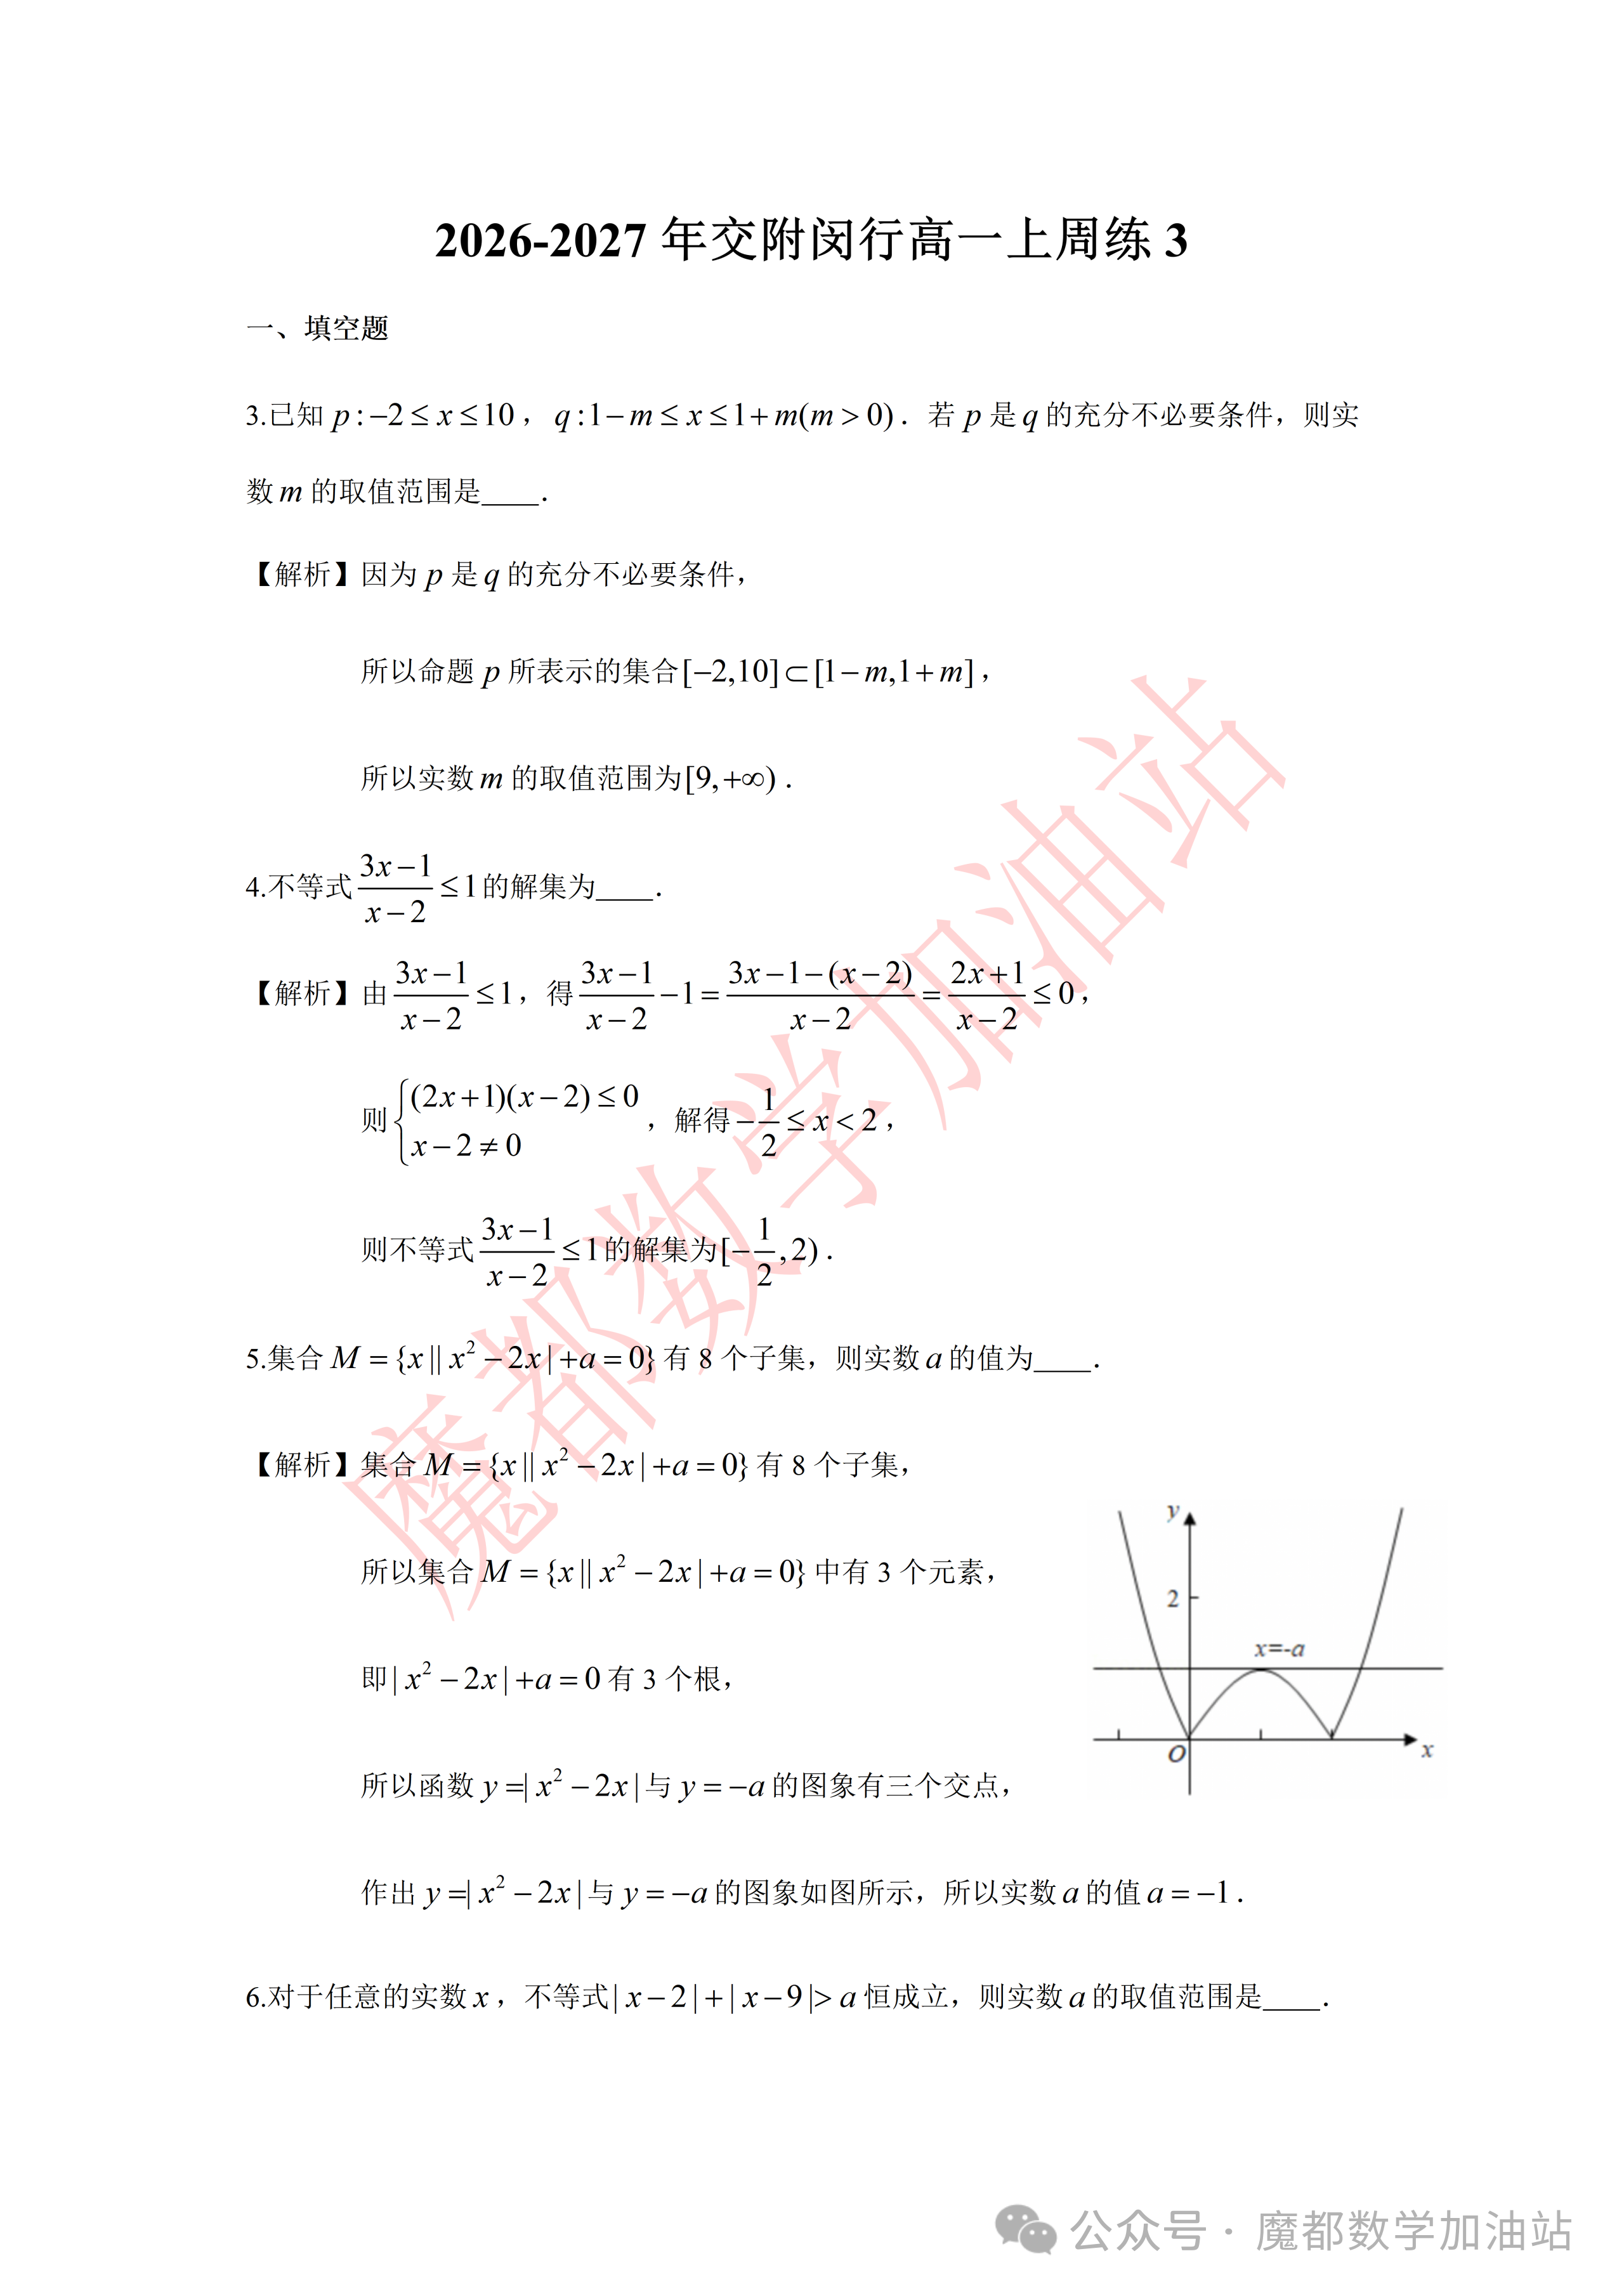
\includegraphics[width=0.14\textwidth,trim={1721bp 837bp 280bp 2297bp},clip]{../原图/高一43_交附闵行_周练3/01.png}
\end{center}

\solbegin
\step{集合 $M=\{x\mid |x^2-2x|+a=0\}$ 有 8 个子集，}
\step{所以集合 $M=\{x\mid |x^2-2x|+a=0\}$ 中有 3 个元素，}
\step{即 $|x^2-2x|+a=0$ 有 3 个根，}
\step{所以函数 $y=|x^2-2x|$ 与 $y=-a$ 的图象有三个交点，}
\step{作出 $y=|x^2-2x|$ 与 $y=-a$ 的图象如图所示，所以实数 $a$ 的值 $a=-1$.}
\solend

\fi

\item 对于任意的实数 $x$，不等式 $|x-2|+|x-9|>a$ 恒成立，则实数 $a$ 的取值范围是 \blankline[4.4em].

\ifanswer
\solbegin
\step{由绝对值的几何意义得 $|x-2|+|x-9|\geqslant7$，当且仅当 $2\leqslant x\leqslant9$ 时等号成立，}
\step{所以 $a<7$，}
\step{即 $a$ 的取值范围为 $(-\infty,7)$.}
\solend

\fi

\item 已知集合 $A=\{x\mid(a-1)x^2+3x-2=0\}$，$B=\{x\mid x^2-3x+2=0\}$，$A\subseteq B$，求实数 $a$ 的取值范围是 \blankline[4.4em].

\ifanswer
\solbegin
\step{由方程 $x^2-3x+2=0$，解得 $x=1$ 或 $x=2$，即 $B=\{1,2\}$，}
\step{因为 $A\subseteq B$，所以 $A=\varnothing$ 或 $A=\{1\}$ 或 $A=\{2\}$ 或 $A=\{1,2\}$，}
\step{当 $A=\varnothing$ 时，$a\neq1$，且 $\Delta=3^2-4(a-1)\times(-2)<0$，解得 $a<-\dfrac18$，}
\step{将 $x=1$ 代入方程 $(a-1)x^2+3x-2=0$，得 $a=0$，}
\step{此时 $A=\{x\mid-x^2+3x-2=0\}=\{1,2\}$，满足条件，}
\step{将 $x=2$ 代入方程 $(a-1)x^2+3x-2=0$，得到 $a=0$，上面已经验证满足条件，}
\step{综上所述，$a$ 的取值范围是 $\left(-\infty,-\dfrac18\right)\cup\{0\}$.}
\solend

\fi

\item 已知 $a$、$b$、$c$、$d$ 为常数，若不等式
$\dfrac{b}{x+a}+\dfrac{x+d}{x+c}<0$ 的解集为 $\left(-1,-\dfrac13\right)\cup\left(\dfrac12,1\right)$，
则不等式 $\dfrac{bx}{ax-1}+\dfrac{dx-1}{cx-1}<0$ 的解集为 \blankline[4.4em].

\ifanswer
\solbegin
\step{若 $x=0$，原不等式化为 $1<0$，不等式显然不成立，所以 $x\neq0$，}
\step{由 $\dfrac{bx}{ax-1}+\dfrac{dx-1}{cx-1}<0$，得 $\dfrac{b}{a-\dfrac1x}+\dfrac{d-\dfrac1x}{c-\dfrac1x}<0$，即 $\dfrac{b}{-\dfrac1x+a}+\dfrac{-\dfrac1x+d}{-\dfrac1x+c}<0$.}
\step{因为不等式 $\dfrac{b}{x+a}+\dfrac{x+d}{x+c}<0$ 的解集为 $\left(-1,-\dfrac13\right)\cup\left(\dfrac12,1\right)$，}
\step{所以 $-1<-\dfrac1x<-\dfrac13$ 或 $\dfrac12<-\dfrac1x<1$，解得 $1<x<3$ 或 $-2<x<-1$，}
\step{所以不等式 $\dfrac{bx}{ax-1}+\dfrac{dx-1}{cx-1}<0$ 的解集为 $(-2,-1)\cup(1,3)$.}
\solend

\fi

\item 正实数 $x$、$y$ 满足 $2x+3y-xy=0$，且存在这样的 $x$、$y$ 使不等式 $x+y<m+1$ 有解，则实数 $m$ 的取值范围是 \blankline[4.4em].

\ifanswer
\solbegin
\step{因为正实数 $x$、$y$ 满足 $2x+3y-xy=0$，则 $\dfrac2y+\dfrac3x=1$，$x>0$，$y>0$，}
\step{所以 $x+y=(x+y)\left(\dfrac3x+\dfrac2y\right)=3+\dfrac{2x}{y}+\dfrac{3y}{x}+2\geqslant2\sqrt{\dfrac{2x}{y}\times\dfrac{3y}{x}}+5=5+2\sqrt6$，}
\step{当且仅当 $\sqrt2x=\sqrt3y$ 时取等号，}
\step{存在这样的 $x$、$y$ 使不等式 $x+y<m+1$ 有解，则 $m+1>5+2\sqrt6$，}
\step{则 $m>4+2\sqrt6$，所以实数 $m$ 的取值范围是 $(4+2\sqrt6,+\infty)$.}
\solend

\fi

\item 若 $a$、$b$、$c\in\R$，$a^2+b^2+c^2=1$，则 $2ab+bc$ 的最大值为 \blankline[4.4em].

\ifanswer
\solbegin
\step{对于 $2ab+bc$，将 $b^2$ 拆分为 $\dfrac45b^2+\dfrac15b^2$，则 $a^2+\dfrac45b^2+c^2+\dfrac15b^2=1$，}
\step{$a^2+\dfrac45b^2\geqslant2\cdot a\cdot\dfrac2{\sqrt5}b=\dfrac4{\sqrt5}ab$，$c^2+\dfrac15b^2\geqslant2\cdot c\cdot\dfrac1{\sqrt5}b=\dfrac2{\sqrt5}bc$，}
\step{两式相加得 $1\geqslant\dfrac4{\sqrt5}ab+\dfrac2{\sqrt5}bc=\dfrac2{\sqrt5}(2ab+bc)$，故 $2ab+bc\leqslant\dfrac{\sqrt5}2$，}
\step{等号成立当且仅当 $a=\dfrac2{\sqrt5}b$，$c=\dfrac1{\sqrt5}b$，}
\step{代入 $a^2+b^2+c^2=1$，得 $\dfrac45b^2+b^2+\dfrac15b^2=2b^2=1$，即 $b=\dfrac{\sqrt2}2$，}
\step{此时 $a=\dfrac{\sqrt{10}}5$，$c=\dfrac{\sqrt{10}}{10}$，故 $2ab+bc$ 的最大值为 $\dfrac{\sqrt5}2$.}
\solend

\fi

\item 已知实数 $a$、$b$ 满足 $-3<a+2b<2$，$-1<2a-b<4$，则 $a+b$ 的取值范围为 \blankline[4.4em].

\ifanswer
\solbegin
\step{设 $a+b=m(a+2b)+n(2a-b)=(m+2n)a+(2m-n)b$，}
\step{所以 $\begin{cases}m+2n=1\\2m-n=1\end{cases}$，解得 $n=\dfrac15$，$m=\dfrac35$，所以 $a+b=\dfrac35(a+2b)+\dfrac15(2a-b)$，}
\step{因为 $-3<a+2b<2$，$-1<2a-b<4$，}
\step{所以 $-\dfrac95<\dfrac35(a+2b)<\dfrac65$，$-\dfrac15<\dfrac15(2a-b)<\dfrac45$，}
\step{相加得 $-2<\dfrac35(a+2b)+\dfrac15(2a-b)<2$，即 $-2<a+b<2$，}
\step{故 $a+b$ 的取值范围为 $(-2,2)$.}
\solend

\fi

% 注：原卷题干与解析均印作 \sqrt{2xyz}，但按其自身答案 8 与取等值（$y=\dfrac12$，
% $x=\dfrac{\sqrt3}4$，$z=\dfrac{\sqrt6}4$）代入只与 $\sqrt{2x^2y^2z^2}=\sqrt2\,xyz$ 相符，
% $\sqrt{2xyz}$ 与答案 8 不自洽，原卷如此，照录未改。
\item 已知正数 $x$、$y$、$z$ 满足 $2x^2+y^2+z^2=1$，则 $\dfrac{y+1}{\sqrt{2xyz}}$ 的最小值为 \blankline[4.4em].

\ifanswer
\solbegin
\step{由条件得 $2x^2+z^2=1-y^2=(1-y)(1+y)$，则 $1+y=\dfrac{2x^2+z^2}{1-y}$，}
\step{结合 $x$、$y$、$z>0$ 得原式 $=\dfrac{2x^2+z^2}{\sqrt{2xyz}(1-y)}\geqslant\dfrac{2\sqrt2xz}{\sqrt{2xyz}(1-y)}=\dfrac2{y(1-y)}$，}
\step{又 $y(1-y)\leqslant\left(\dfrac{y+1-y}2\right)^2=\dfrac14$，所以 $\dfrac2{y(1-y)}\geqslant\dfrac2{\frac14}=8$，}
\step{当且仅当 $\sqrt2x=z$，且 $y=1-y$，即 $y=\dfrac12$，$x=\dfrac{\sqrt3}4$，$z=\dfrac{\sqrt6}4$ 时取等号，}
\step{故 $\dfrac{y+1}{\sqrt{2xyz}}$ 最小值为 $8$.}
\solend

\fi

\end{enumerate}

\bigsec{二、选择题}

\begin{enumerate}
\setcounter{enumi}{12}

\item 已知关于 $x$ 的方程 $(1-k)x^2-2x-1=0$ 有实数根，则 $k$ 的取值范围是\mbox{（\quad）}

\keepwithprev
A. $k\leqslant2$ 且 $k\neq1$\qquad B. $k\leqslant2$\qquad
C. $k<2$ 且 $k\neq1$\qquad D. $k<2$

\ans{$A$}

\ifanswer
\solbegin
\step{由题意得 $\begin{cases}1-k\neq0\\\Delta=4+4(1-k)\geqslant0\end{cases}$，解不等式得 $\begin{cases}1\neq k\\2-k>0\end{cases}$，所以 $k\leqslant2$ 且 $k\neq1$，}
\step{故选 $A$.}
\solend

\fi

\item 不等式 $2|x+2|+|x-1|\geqslant5$ 成立的一个必要不充分条件是\mbox{（\quad）}

\keepwithprev
A. $x\leqslant-1$ 或 $x\geqslant0$\qquad B. $x\geqslant0$

C. $x\leqslant-\dfrac83$ 或 $x\geqslant0$\qquad D. $x\geqslant1$

\ans{$A$}

\ifanswer
\solbegin
\step{当 $x<-2$ 时，原不等式可化为 $-2x-4-x+1\geqslant5$，解得 $x\leqslant-\dfrac83$，}
\step{当 $-2\leqslant x<1$ 时，原不等式可化为 $2x+4-x+1\geqslant5$，解得 $0\leqslant x<1$，}
\step{当 $x\geqslant1$ 时，原不等式可化为 $2x+4+x-1\geqslant5$，解得 $x\geqslant\dfrac23$，得 $x\geqslant1$，}
\step{综上所述，不等式 $2|x+2|+|x-1|\geqslant5$ 成立的充要条件是 $x\leqslant-\dfrac83$ 或 $x\geqslant0$，}
\step{设 $A=\{x\mid x\leqslant-\dfrac83\text{ 或 }x\geqslant0\}$，}
\step{则不等式 $2|x+2|+|x-1|\geqslant5$ 成立的必要不充分条件，}
\step{其对应的集合 $B$ 满足 $A\subsetneq B$，对照各个选项，$A$ 项符合题意. 故选 $A$.}
\solend

\fi

\item 已知实数 $a>0$，$b>0$，$\dfrac1{a+1}+\dfrac1{b+1}=1$，则 $2a+3b$ 的最小值为\mbox{（\quad）}

\keepwithprev
A. $2\sqrt6$\qquad B. $3+2\sqrt6$\qquad
C. $5+2\sqrt6$\qquad D. $3+2\sqrt2$

\ans{$A$}

\ifanswer
\solbegin
\step{因为 $a>0$，$b>0$，$\dfrac1{a+1}+\dfrac1{b+1}=1$，}
\step{所以 $2a+3b=2(a+1)+3(b+1)-5=[2(a+1)+3(b+1)]\cdot\left(\dfrac1{a+1}+\dfrac1{b+1}\right)-5$}
\step{$=\left[2+3+\dfrac{3(b+1)}{a+1}+\dfrac{2(a+1)}{b+1}\right]-5\geqslant5+2\sqrt{\dfrac{3(b+1)}{a+1}\times\dfrac{2(a+1)}{b+1}}-5=2\sqrt6$，}
\step{当且仅当 $\dfrac{3(b+1)}{a+1}=\dfrac{2(a+1)}{b+1}$，即 $a=\dfrac{\sqrt6}2$，$b=\dfrac{\sqrt6}3$ 时取等号. 故选 $A$.}
\solend

\fi

\item 已知集合 $U=\{n\mid1\leqslant n\leqslant2027,\ n\in\N\}$，集合 $M\subseteq U$，若对于 $M$ 中任意两个不同的元素 $x$ 和 $y$，都有 $|x-y|>2$，则 $M$ 中元素个数的最大值是\mbox{（\quad）}

\keepwithprev
A. $676$\qquad B. $675$\qquad C. $672$\qquad D. $671$

\ans{$A$}

\ifanswer
\solbegin
\step{对于 $M$ 中的任意两个不同的元素 $x$、$y$，都有 $|x-y|>2$，}
\step{不妨设 $x>y$，都有 $x-y\geqslant3$，}
\step{要想 $M$ 所含元素个数最大，则要 $x-y$ 尽可能小，故需使得 $x-y$ 的最小值为 3，}
\step{将 $1\sim2027$ 这 2027 个元素按如下分组：}
\step{$\{1,2,3\}$，$\{4,5,6\}$，$\cdots$，$\{2023,2024,2025\}$，$\{2026,2027\}$，}
\step{故应在前 675 组中按周期 3 每组取一个元素，且第一组中不能取 3，}
\step{第一组中取 1 时，得 $M=\{1,4,7,\cdots,2023,2026\}$，}
\step{或 $M=\{1,4,7,\cdots,2023,2027\}$ 这样的集合，}
\step{第一组取 2 时，得 $M=\{2,5,8,\cdots,2024,2027\}$，}
\step{其中任意两元素差值 $x-y$（$x>y$）都大于 2，满足题意，}
\step{故 $M$ 所含元素个数的最大值为 $\dfrac{2025}{3}+1=676$. 故选 $A$.}
\solend

\fi

\end{enumerate}

\bigsec{三、解答题}

\begin{enumerate}
\setcounter{enumi}{16}

\item 已知 $a\in\R$，集合 $A=\left\{x\middle|\dfrac{2-x}{x+1}\leqslant0\right\}$，$B=\{x\mid x^2+(3-a)x-3a<0\}$.

\begin{enumerate}[label=(\arabic*)]
\item 当 $a=\dfrac13$ 时，求 $A$ 和 $B$；
\item 已知 $A\cup B=A$，求实数 $a$ 的取值范围.
\end{enumerate}

\ifanswer
\solbegin
\stepm{(1)}{由 $\dfrac{2-x}{x+1}\leqslant0$，得 $\begin{cases}(2-x)(x+1)\leqslant0\\x\neq-1\end{cases}$，解得 $x<-1$ 或 $x\geqslant2$，}
\step{则 $A=\{x\mid x<-1\text{ 或 }x\geqslant2\}$；}
\step{$B=\{x\mid x^2+(3-a)x-3a<0\}=\{x\mid(x+3)(x-a)<0\}$，}
% 注：原卷此行印作 $(x+2)\left(x-\dfrac13\right)$，按前一行 $B=\{x\mid(x+3)(x-a)<0\}$ 应为
% $(x+3)\left(x-\dfrac13\right)$，原卷如此，照录未改。
\step{当 $a=\dfrac13$ 时，$B=\left\{x\middle|(x+2)\left(x-\dfrac13\right)<0\right\}$，}
\step{解得 $B=\left\{x\middle|-3<x<\dfrac13\right\}$.}
\stepm{(2)}{由 $A\cup B=A$，得 $B\subseteq A$，}
\step{①当 $B=\varnothing$ 时，得 $a=-3$，符合题意；}
\step{②当 $B\neq\varnothing$ 时，若 $a>-3$，则 $B=\{x\mid-3<x<a\}$，}
\step{由 $B\subseteq A$，得 $a\leqslant-1$，此时 $-3<a\leqslant-1$；}
\step{若 $a<-3$，则 $B=\{x\mid a<x<-3\}$，此时 $B\subseteq A$ 恒成立，}
\step{故 $a<-3$ 符合题意；}
\step{综上所述，实数 $a$ 的取值范围为 $a\leqslant-1$.}
\solend

\fi

\ansspace[6]

\item 甲乙两地的高速公路全长 166 千米，汽车从甲地进入该高速公路后匀速行驶到乙地，车速 $v\in[70,120]$（千米/时）. 已知汽车每小时的运输成本（以元为单位）由可变部分和固定部分组成：可变部分为 $0.02v^2$，固定部分为 220 元.

\begin{enumerate}[label=(\arabic*)]
\item 若每小时的运输成本不高于 420 元，汽车的速度应该控制在什么范围？
\item 汽车应以多大速度行驶才能使全程运输成本最小？最小运输成本约为多少元？（结果保留整数）
\end{enumerate}

\ifanswer
\solbegin
\stepm{(1)}{已知汽车每小时的运输成本（以元为单位）由可变部分和固定部分组成：}
\step{可变部分为 $0.02v^2$，固定部分为 220 元，}
\step{则汽车每小时的运输成本为 $0.02v^2+220$（元），}
\step{若每小时的运输成本不高于 420 元，}
\step{则 $0.02v^2+220\leqslant420$，解得 $v^2\leqslant10000$，}
\step{得 $70\leqslant v\leqslant100$，即 $v\in[70,100]$（千米/时），}
\step{则此时汽车的速度 $v$ 应该控制在 $[70,100]$（千米/时）；}
\stepm{(2)}{因为汽车从甲地进入该高速公路后匀速行驶到乙地，}
\step{车速 $v\in[70,120]$（千米/时），所以汽车的行驶时间为 $\dfrac{166}{v}$（小时），}
\step{所以全程运输成本 $y=\dfrac{166}{v}(0.02v^2+220)=3.32v+\dfrac{36520}{v}$，}
% 注：原卷此行印作 $v\in[70,100]$，与题干的 $v\in[70,120]$ 不自洽（若 $v\in[70,100]$，
% 最小值应在 $v=100$ 处取得，与下文 $v=10\sqrt{110}\approx105$ 矛盾），原卷如此，照录未改。
\step{$v\in[70,100]$，}
\step{由基本不等式得 $y=3.32v+\dfrac{36520}{v}\geqslant2\sqrt{3.32v\times\dfrac{36520}{v}}\approx696$，}
\step{当且仅当 $3.32v=\dfrac{36520}{v}$，即 $v=10\sqrt{110}\approx105$ 时取等号，}
\step{汽车应以 105（千米/时）行驶才能使全程运输成本最小，}
\step{最小运输成本约为 696 元.}
\solend

\fi

\ansspace[8]

\item
\begin{enumerate}[label=(\arabic*)]
\item 已知 $a$、$b$、$c$ 为实数，求证：$|a-b|\leqslant|a-c|+|b-c|$，并说明等号成立的条件；
\item 设 $x\in\R$，求方程 $|3x-8|=|5-x|+|2x-3|$ 的解集.
\end{enumerate}

\ifanswer
% 注：原卷第 19 题未印【解析】，仅印一行【答案】"（1）(a-c)(b-c)≤0；
% （2）(-∞,3/2]∪[5,+∞)"。(1) 的两行推导为本稿所补，(2) 照录原卷答案。
% 又题干作"方程"，而所给答案 (-∞,3/2]∪[5,+∞) 实为不等式 |3x-8|≤|5-x|+|2x-3| 的解集，
% 与"方程"不合，原卷如此，照录未改。
\solbegin
\stepm{(1)}{由三角不等式 $|a-b|=|(a-c)-(b-c)|\leqslant|a-c|+|b-c|$，}
\step{当且仅当 $(a-c)(b-c)\leqslant0$ 时等号成立.}
\stepm{(2)}{$\left(-\infty,\dfrac32\right]\cup[5,+\infty)$.}
\solend

\fi

\ansspace[6]

\item 已知正实数 $a$、$b$ 满足 $a+b=1$，求 $\dfrac1a+\dfrac1b$ 的最小值. 其中一种解法是：

\[
\begin{aligned}
\dfrac1a+\dfrac1b
&=\left(\dfrac1a+\dfrac1b\right)(a+b)\\
&=1+\dfrac ba+\dfrac ab+1\\
&\geqslant2+2\sqrt{\dfrac ba\times\dfrac ab}=2+2=4.
\end{aligned}
\]
当且仅当 $\dfrac ba=\dfrac ab$ 且 $a+b=1$ 时即 $a=b=\dfrac12$ 时取等号.
学习上述解法并解决下列问题：

\begin{enumerate}[label=(\arabic*)]
\item 若正实数 $x$、$y$ 满足 $x+y=xy$，求 $2x+y$ 的最小值；
\item 若实数 $a$、$b$、$x$、$y$ 满足 $\dfrac{x^2}{a^2}+\dfrac{y^2}{b^2}=1$，求证：$a^2+b^2\geqslant(x+y)^2$；
\item 求代数式 $M=\sqrt{m-1}+\sqrt{3-m}$ 的最大值，并求出使得 $M$ 最大的 $m$ 的值.
\end{enumerate}

\ifanswer
\solbegin
\stepm{(1)}{因为正实数 $x$、$y$ 满足 $x+y=xy$，$\dfrac{x+y}{xy}=1\Rightarrow\dfrac1y+\dfrac1x=1$，}
\step{所以 $(2x+y)\times1=(2x+y)\left(\dfrac1y+\dfrac1x\right)=3+\dfrac{2x}{y}+\dfrac yx\geqslant3+2\sqrt{\dfrac{2x}{y}\cdot\dfrac yx}=3+2\sqrt2$，}
\step{当且仅当 $\dfrac{2x}{y}=\dfrac yx$ 且 $\dfrac1y+\dfrac1x=1$ 时取等号，}
\step{解得 $x=\dfrac{2+\sqrt2}2$，$y=\sqrt2x=\sqrt2\times\dfrac{2+\sqrt2}2=1+\sqrt2$，}
\step{所以 $2x+y$ 的最小值为 $3+2\sqrt2$；}
\stepm{(2)}{因为 $\dfrac{x^2}{a^2}+\dfrac{y^2}{b^2}=1$，}
\step{所以 $a^2+b^2=(a^2+b^2)\left(\dfrac{x^2}{a^2}+\dfrac{y^2}{b^2}\right)=x^2+y^2+\dfrac{b^2x^2}{a^2}+\dfrac{a^2y^2}{b^2}$，}
\step{因为 $\dfrac{b^2x^2}{a^2}+\dfrac{a^2y^2}{b^2}\geqslant2\sqrt{\dfrac{b^2x^2}{a^2}\times\dfrac{a^2y^2}{b^2}}=2\sqrt{x^2y^2}=2|xy|$，}
\step{当且仅当 $\dfrac{b^2x^2}{a^2}=\dfrac{a^2y^2}{b^2}$ 时取等号，}
\step{所以 $x^2+y^2+\dfrac{b^2x^2}{a^2}+\dfrac{a^2y^2}{b^2}\geqslant x^2+y^2+2|xy|\geqslant x^2+y^2+2xy=(x+y)^2$，}
\step{所以 $a^2+b^2\geqslant(x+y)^2$；}
\stepm{(3)}{因为 $M=\sqrt{m-1}+\sqrt{3-m}$，所以 $\begin{cases}m-1\geqslant0\\3-m\geqslant0\end{cases}$，解得 $1\leqslant m\leqslant3$，}
\step{所以 $M^2=(\sqrt{m-1}+\sqrt{3-m})^2=2+2\sqrt{(3-m)(m-1)}$，}
\step{由基本不等式得 $(3-m)(m-1)\leqslant\left(\dfrac{(3-m)+(m-1)}2\right)^2=1$，}
\step{当且仅当 $3-m=m-1$ 时取等号，解得 $m=2$，}
\step{所以 $M^2=2+2\sqrt{(3-m)(m-1)}\leqslant2+2\sqrt1=4$，}
\step{因为 $M>0$，所以 $M\leqslant2$，所以 $M$ 最大值为 2，此时 $m$ 的值为 2.}
\solend

\fi

\ansspace[8]

\item 若有限个正整数组成的集合 $A$ 中至少有两个元素，且对于任意的 $x,y\in A$（$x>y$），都有 $\dfrac{y^2}{x-y}\in A$，则称 $A$ 为“L-集合”.

\begin{enumerate}[label=(\arabic*)]
\item 判断 $\{1,2,4\}$ 是否为“L-集合”，说明理由；
\item 若双元素集 $M$ 为“L-集合”，且 $4\in M$，求所有满足条件的集合 $M$；
\item 求所有满足条件的“L-集合”.
\end{enumerate}

\ifanswer
\solbegin
\stepm{(1)}{若至少由两个元素构成的有限集合 $A\subseteq\N^*$，}
% 注：原卷下一行"都有"后未印分数 \dfrac{y^2}{x-y}，径作"都有 A"，原卷如此，照录未改。
\step{且对于任意的 $x$、$y\in A$（$x>y$），都有 $A$，则称 $A$ 为“L-集合”，}
\step{$\{1,2,4\}$ 不为“L-集合”，理由如下：}
\step{因为 $\dfrac{1^2}{4-1}=\dfrac13\notin\{1,2,4\}$，所以 $\{1,2,4\}$ 不是“L-集合”.}
\stepm{(2)}{设 $M=\{4,m\}$（$m\in\N^*$，$m\neq4$），}
\step{若 $m<4$，则 $\dfrac{m^2}{4-m}=m$ 或 $\dfrac{m^2}{4-m}=4$，}
\step{由 $\dfrac{m^2}{4-m}=m$，解得 $m=2$，$m=0$（舍去），此时 $M=\{2,4\}$；}
\step{由 $\dfrac{m^2}{4-m}=4$ 化为 $m^2+4m-16=0$，而 $\Delta=4^2+4\times16=80$，}
\step{故方程无正整数解.}
\step{若 $m>4$，则 $\dfrac{4^2}{m-4}=4$ 或 $\dfrac{4^2}{m-4}=m$，}
\step{由 $\dfrac{4^2}{m-4}=4$，解得 $m=8$，此时 $M=\{4,8\}$；}
\step{由 $\dfrac{4^2}{m-4}=m$ 化为 $m^2-4m-16=0$，而 $\Delta=4^2+4\times16=80$，}
\step{故方程无正整数解.}
\step{综上，双元素集 $M$ 为“L-集合”，且 $4\in M$，}
\step{则所有满足条件的集合 $M$ 为 $\{4,8\}$，$\{2,4\}$.}
\stepm{(3)}{若“L-集合”为双元素集，}
\step{不妨设 $M=\{k,m\}$（$k,m\in\N^*$，$m>k$），则 $\dfrac{k^2}{m-k}=k$ 或 $\dfrac{k^2}{m-k}=m$，}
\step{由 $\dfrac{k^2}{m-k}=k$，则 $2k^2=mk$，而 $m>k$，故 $m=2k$，此时 $M=\{k,2k\}$；}
\step{由 $\dfrac{k^2}{m-k}=m$，则 $m^2-mk-k^2=0$，而 $\Delta=5k^2$，显然不存在正整数解；}
\step{所以，“L-集合”为 $\{k,2k\}$，其中 $k\in\N^*$.}
\step{若“L-集合”含有两个以上的元素，}
\step{设最小的元素为 $b$，最大的元素为 $a$，第二大的元素为 $n$，}
\step{则 $\dfrac{b^2}{a-b}$，$\dfrac{n^2}{a-n}$ 是“L-集合”中的元素，}
% 注：原卷下一行未印"由于'L-集合'中的元素均为正整数"一语，径作"若 \dfrac{b^2}{a-b}\geqslant b"，
% 原卷如此，照录未改。
\step{若 $\dfrac{b^2}{a-b}\geqslant b$，解得 $a\leqslant2b$，}
\step{若 $\dfrac{n^2}{a-n}\leqslant n$，则 $a\geqslant2n>2b$，矛盾，}
\step{若 $\dfrac{n^2}{a-n}=a$，该方程的解为 $n=\dfrac{\sqrt5-1}2a$，则 $n$、$a$ 不可能同时为整数，}
\step{无解.}
\step{所以所有满足条件的“L-集合”为 $\{k,2k\}$，其中 $k\in\N^*$.}
\solend

\fi

\ansspace*[10]

\end{enumerate}

\end{document}
"
%
% 原始材料是微信公众号图文（公众号“魔都数学加油站”，作者破晓，2026-10-01 21:37，
% 原文标题“27学年高一43——2026-2027年上海市交附闵行高一上周练3”，
% https://mp.weixin.qq.com/s/-rgkOD9jJVpug6s0uSbwmQ）。正文为 12 张 PNG 页；
% 第 01、05、09、12 页 2560×3620，其余第 02—04、06—08、10—11 页 4762×6735。
% 原文本身是讲评版，题目下方印有解析/答案；题目与讲解照原卷转录，保留原卷错误。
%
% 卷首标题：原卷印作“2026-2027 年交附闵行高一上周练3”，公众号标题中的“上海市”
% 三字不在卷面标题中，本稿依卷面录入；年份区间按全稿惯例排 en dash。
%
% 与原卷的排版差异：
%   ① 原文从第 3 题开始（第 1、2 题未在这篇推文中发布），本稿保留原题号 3—21；
%   ② 原卷本就印有“一、填空题”“二、选择题”“三、解答题”，本稿照原卷分节，
%      改排为全稿统一的大节标题；
%   ③ 原卷未印副标题，本稿按“知识模块”口径补出“集合与常用逻辑用语、不等式”；
%   ④ 原卷填空横线依全稿惯例排为 \blankline[4.4em]；选择题答案只在答案版以 \ans{} 显示，
%      解答区以 \ifanswer 分离；解答题按原卷留出标准作答空间；
%   ⑤ 第 5 题图取自原卷第 1 页截图并裁入本稿，不另建图档；公众号水印不录入。
%      原卷图页分页不保留，正文依本稿版心重新分页。
%
% 原卷存疑/错误（均照录，未改）：
%   ① 第 9 题原卷题干即作"正实数 x、y"，与解析 x>0、y>0 相容，并无矛盾（初稿曾误记
%      题干只称"实数"并据此指原卷不自洽，2026-10-05 回原图核对订正）。
%   ② 第 11 题解析"相加得"一行原卷印作 -2<3/5(a+2b)+1/5(2a-b)<2，第一项系数 3/5
%      原卷不缺（初稿漏抄致该行按字面不成立，2026-10-05 已按原卷补回）。
%   ③ 第 13 题答案印 A，解析以“1-k≠0”排除 k=1；但 k=1 时原方程为 -2x-1=0，
%      仍有实数根，按题意应选 B。本稿保留原卷答案 A 及其解析，不代为订正。
%
\documentclass[a4paper,11pt]{article}
\usepackage{common}
\usepackage{graphicx}

\begin{document}

\examtitlest[3]{2026--2027 年交附闵行高一上周练 3}{集合与常用逻辑用语、不等式}

\bigsec{一、填空题}

\begin{enumerate}
\setcounter{enumi}{2}

\item 已知 $p\colon -2\leqslant x\leqslant10$，$q\colon 1-m\leqslant x\leqslant1+m$（$m>0$）. 若 $p$ 是 $q$ 的充分不必要条件，则实数 $m$ 的取值范围是 \blankline[4.4em].

\ifanswer
\solbegin
\step{因为 $p$ 是 $q$ 的充分不必要条件，}
\step{所以命题 $p$ 所表示的集合 $[-2,10]\subset[1-m,1+m]$，}
\step{所以实数 $m$ 的取值范围为 $[9,+\infty)$.}
\solend

\fi

\item 不等式 $\dfrac{3x-1}{x-2}\leqslant1$ 的解集为 \blankline[4.4em].

\ifanswer
\solbegin
\step{由 $\dfrac{3x-1}{x-2}-1=\dfrac{3x-1-(x-2)}{x-2}=\dfrac{2x+1}{x-2}\leqslant0$，}
\step{则 $\begin{cases}(2x+1)(x-2)\leqslant0\\x-2\neq0\end{cases}$，解得 $-\dfrac12\leqslant x<2$，}
\step{则不等式 $\dfrac{3x-1}{x-2}\leqslant1$ 的解集为 $\left[-\dfrac12,2\right)$.}
\solend

\fi

\item 集合 $M=\{x\mid |x^2-2x|+a=0\}$ 有 8 个子集，则实数 $a$ 的值为 \blankline[4.4em].

\ifanswer
\begin{center}
% 图取自原卷第 1 页；用原图裁切，未重绘。
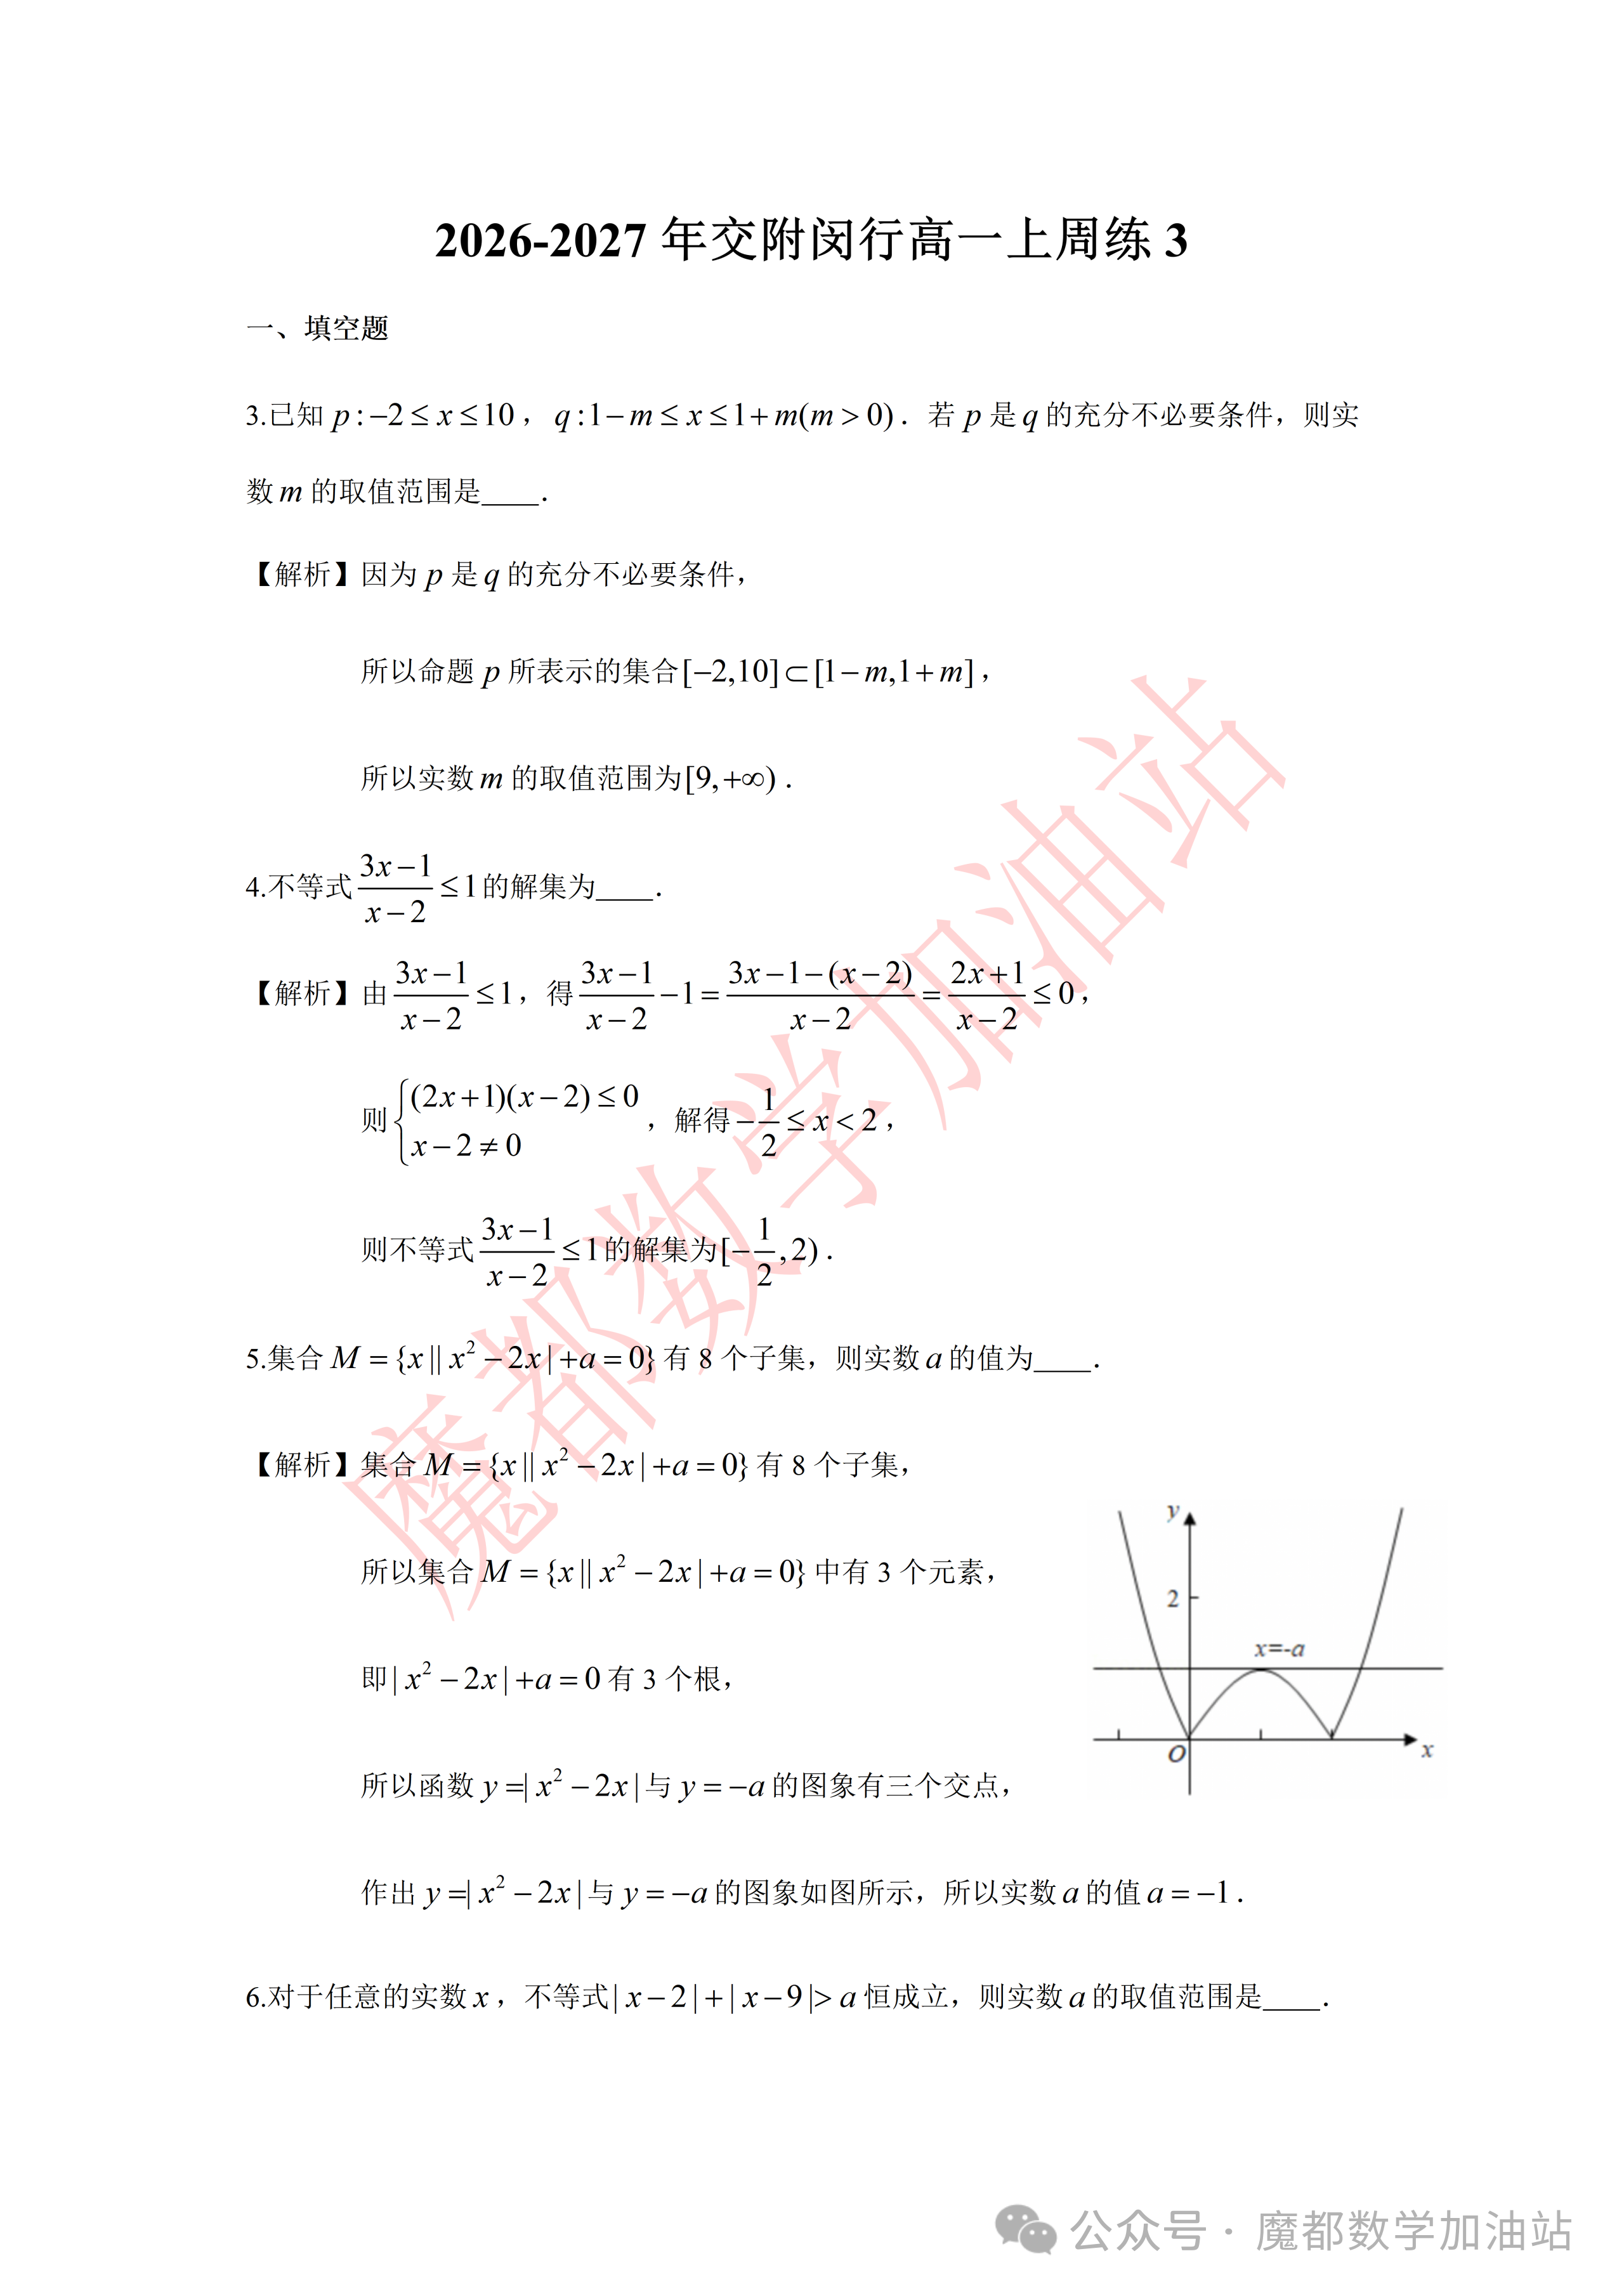
\includegraphics[width=0.14\textwidth,trim={1721bp 837bp 280bp 2297bp},clip]{../原图/高一43_交附闵行_周练3/01.png}
\end{center}

\solbegin
\step{集合 $M=\{x\mid |x^2-2x|+a=0\}$ 有 8 个子集，}
\step{所以集合 $M=\{x\mid |x^2-2x|+a=0\}$ 中有 3 个元素，}
\step{即 $|x^2-2x|+a=0$ 有 3 个根，}
\step{所以函数 $y=|x^2-2x|$ 与 $y=-a$ 的图象有三个交点，}
\step{作出 $y=|x^2-2x|$ 与 $y=-a$ 的图象如图所示，所以实数 $a$ 的值 $a=-1$.}
\solend

\fi

\item 对于任意的实数 $x$，不等式 $|x-2|+|x-9|>a$ 恒成立，则实数 $a$ 的取值范围是 \blankline[4.4em].

\ifanswer
\solbegin
\step{由绝对值的几何意义得 $|x-2|+|x-9|\geqslant7$，当且仅当 $2\leqslant x\leqslant9$ 时等号成立，}
\step{所以 $a<7$，}
\step{即 $a$ 的取值范围为 $(-\infty,7)$.}
\solend

\fi

\item 已知集合 $A=\{x\mid(a-1)x^2+3x-2=0\}$，$B=\{x\mid x^2-3x+2=0\}$，$A\subseteq B$，求实数 $a$ 的取值范围是 \blankline[4.4em].

\ifanswer
\solbegin
\step{由方程 $x^2-3x+2=0$，解得 $x=1$ 或 $x=2$，即 $B=\{1,2\}$，}
\step{因为 $A\subseteq B$，所以 $A=\varnothing$ 或 $A=\{1\}$ 或 $A=\{2\}$ 或 $A=\{1,2\}$，}
\step{当 $A=\varnothing$ 时，$a\neq1$，且 $\Delta=3^2-4(a-1)\times(-2)<0$，解得 $a<-\dfrac18$，}
\step{将 $x=1$ 代入方程 $(a-1)x^2+3x-2=0$，得 $a=0$，}
\step{此时 $A=\{x\mid-x^2+3x-2=0\}=\{1,2\}$，满足条件，}
\step{将 $x=2$ 代入方程 $(a-1)x^2+3x-2=0$，得到 $a=0$，上面已经验证满足条件，}
\step{综上所述，$a$ 的取值范围是 $\left(-\infty,-\dfrac18\right)\cup\{0\}$.}
\solend

\fi

\item 已知 $a$、$b$、$c$、$d$ 为常数，若不等式
$\dfrac{b}{x+a}+\dfrac{x+d}{x+c}<0$ 的解集为 $\left(-1,-\dfrac13\right)\cup\left(\dfrac12,1\right)$，
则不等式 $\dfrac{bx}{ax-1}+\dfrac{dx-1}{cx-1}<0$ 的解集为 \blankline[4.4em].

\ifanswer
\solbegin
\step{若 $x=0$，原不等式化为 $1<0$，不等式显然不成立，所以 $x\neq0$，}
\step{由 $\dfrac{bx}{ax-1}+\dfrac{dx-1}{cx-1}<0$，得 $\dfrac{b}{a-\dfrac1x}+\dfrac{d-\dfrac1x}{c-\dfrac1x}<0$，即 $\dfrac{b}{-\dfrac1x+a}+\dfrac{-\dfrac1x+d}{-\dfrac1x+c}<0$.}
\step{因为不等式 $\dfrac{b}{x+a}+\dfrac{x+d}{x+c}<0$ 的解集为 $\left(-1,-\dfrac13\right)\cup\left(\dfrac12,1\right)$，}
\step{所以 $-1<-\dfrac1x<-\dfrac13$ 或 $\dfrac12<-\dfrac1x<1$，解得 $1<x<3$ 或 $-2<x<-1$，}
\step{所以不等式 $\dfrac{bx}{ax-1}+\dfrac{dx-1}{cx-1}<0$ 的解集为 $(-2,-1)\cup(1,3)$.}
\solend

\fi

\item 正实数 $x$、$y$ 满足 $2x+3y-xy=0$，且存在这样的 $x$、$y$ 使不等式 $x+y<m+1$ 有解，则实数 $m$ 的取值范围是 \blankline[4.4em].

\ifanswer
\solbegin
\step{因为正实数 $x$、$y$ 满足 $2x+3y-xy=0$，则 $\dfrac2y+\dfrac3x=1$，$x>0$，$y>0$，}
\step{所以 $x+y=(x+y)\left(\dfrac3x+\dfrac2y\right)=3+\dfrac{2x}{y}+\dfrac{3y}{x}+2\geqslant2\sqrt{\dfrac{2x}{y}\times\dfrac{3y}{x}}+5=5+2\sqrt6$，}
\step{当且仅当 $\sqrt2x=\sqrt3y$ 时取等号，}
\step{存在这样的 $x$、$y$ 使不等式 $x+y<m+1$ 有解，则 $m+1>5+2\sqrt6$，}
\step{则 $m>4+2\sqrt6$，所以实数 $m$ 的取值范围是 $(4+2\sqrt6,+\infty)$.}
\solend

\fi

\item 若 $a$、$b$、$c\in\R$，$a^2+b^2+c^2=1$，则 $2ab+bc$ 的最大值为 \blankline[4.4em].

\ifanswer
\solbegin
\step{对于 $2ab+bc$，将 $b^2$ 拆分为 $\dfrac45b^2+\dfrac15b^2$，则 $a^2+\dfrac45b^2+c^2+\dfrac15b^2=1$，}
\step{$a^2+\dfrac45b^2\geqslant2\cdot a\cdot\dfrac2{\sqrt5}b=\dfrac4{\sqrt5}ab$，$c^2+\dfrac15b^2\geqslant2\cdot c\cdot\dfrac1{\sqrt5}b=\dfrac2{\sqrt5}bc$，}
\step{两式相加得 $1\geqslant\dfrac4{\sqrt5}ab+\dfrac2{\sqrt5}bc=\dfrac2{\sqrt5}(2ab+bc)$，故 $2ab+bc\leqslant\dfrac{\sqrt5}2$，}
\step{等号成立当且仅当 $a=\dfrac2{\sqrt5}b$，$c=\dfrac1{\sqrt5}b$，}
\step{代入 $a^2+b^2+c^2=1$，得 $\dfrac45b^2+b^2+\dfrac15b^2=2b^2=1$，即 $b=\dfrac{\sqrt2}2$，}
\step{此时 $a=\dfrac{\sqrt{10}}5$，$c=\dfrac{\sqrt{10}}{10}$，故 $2ab+bc$ 的最大值为 $\dfrac{\sqrt5}2$.}
\solend

\fi

\item 已知实数 $a$、$b$ 满足 $-3<a+2b<2$，$-1<2a-b<4$，则 $a+b$ 的取值范围为 \blankline[4.4em].

\ifanswer
\solbegin
\step{设 $a+b=m(a+2b)+n(2a-b)=(m+2n)a+(2m-n)b$，}
\step{所以 $\begin{cases}m+2n=1\\2m-n=1\end{cases}$，解得 $n=\dfrac15$，$m=\dfrac35$，所以 $a+b=\dfrac35(a+2b)+\dfrac15(2a-b)$，}
\step{因为 $-3<a+2b<2$，$-1<2a-b<4$，}
\step{所以 $-\dfrac95<\dfrac35(a+2b)<\dfrac65$，$-\dfrac15<\dfrac15(2a-b)<\dfrac45$，}
\step{相加得 $-2<\dfrac35(a+2b)+\dfrac15(2a-b)<2$，即 $-2<a+b<2$，}
\step{故 $a+b$ 的取值范围为 $(-2,2)$.}
\solend

\fi

% 注：原卷题干与解析均印作 \sqrt{2xyz}，但按其自身答案 8 与取等值（$y=\dfrac12$，
% $x=\dfrac{\sqrt3}4$，$z=\dfrac{\sqrt6}4$）代入只与 $\sqrt{2x^2y^2z^2}=\sqrt2\,xyz$ 相符，
% $\sqrt{2xyz}$ 与答案 8 不自洽，原卷如此，照录未改。
\item 已知正数 $x$、$y$、$z$ 满足 $2x^2+y^2+z^2=1$，则 $\dfrac{y+1}{\sqrt{2xyz}}$ 的最小值为 \blankline[4.4em].

\ifanswer
\solbegin
\step{由条件得 $2x^2+z^2=1-y^2=(1-y)(1+y)$，则 $1+y=\dfrac{2x^2+z^2}{1-y}$，}
\step{结合 $x$、$y$、$z>0$ 得原式 $=\dfrac{2x^2+z^2}{\sqrt{2xyz}(1-y)}\geqslant\dfrac{2\sqrt2xz}{\sqrt{2xyz}(1-y)}=\dfrac2{y(1-y)}$，}
\step{又 $y(1-y)\leqslant\left(\dfrac{y+1-y}2\right)^2=\dfrac14$，所以 $\dfrac2{y(1-y)}\geqslant\dfrac2{\frac14}=8$，}
\step{当且仅当 $\sqrt2x=z$，且 $y=1-y$，即 $y=\dfrac12$，$x=\dfrac{\sqrt3}4$，$z=\dfrac{\sqrt6}4$ 时取等号，}
\step{故 $\dfrac{y+1}{\sqrt{2xyz}}$ 最小值为 $8$.}
\solend

\fi

\end{enumerate}

\bigsec{二、选择题}

\begin{enumerate}
\setcounter{enumi}{12}

\item 已知关于 $x$ 的方程 $(1-k)x^2-2x-1=0$ 有实数根，则 $k$ 的取值范围是\mbox{（\quad）}

\keepwithprev
A. $k\leqslant2$ 且 $k\neq1$\qquad B. $k\leqslant2$\qquad
C. $k<2$ 且 $k\neq1$\qquad D. $k<2$

\ans{$A$}

\ifanswer
\solbegin
\step{由题意得 $\begin{cases}1-k\neq0\\\Delta=4+4(1-k)\geqslant0\end{cases}$，解不等式得 $\begin{cases}1\neq k\\2-k>0\end{cases}$，所以 $k\leqslant2$ 且 $k\neq1$，}
\step{故选 $A$.}
\solend

\fi

\item 不等式 $2|x+2|+|x-1|\geqslant5$ 成立的一个必要不充分条件是\mbox{（\quad）}

\keepwithprev
A. $x\leqslant-1$ 或 $x\geqslant0$\qquad B. $x\geqslant0$

C. $x\leqslant-\dfrac83$ 或 $x\geqslant0$\qquad D. $x\geqslant1$

\ans{$A$}

\ifanswer
\solbegin
\step{当 $x<-2$ 时，原不等式可化为 $-2x-4-x+1\geqslant5$，解得 $x\leqslant-\dfrac83$，}
\step{当 $-2\leqslant x<1$ 时，原不等式可化为 $2x+4-x+1\geqslant5$，解得 $0\leqslant x<1$，}
\step{当 $x\geqslant1$ 时，原不等式可化为 $2x+4+x-1\geqslant5$，解得 $x\geqslant\dfrac23$，得 $x\geqslant1$，}
\step{综上所述，不等式 $2|x+2|+|x-1|\geqslant5$ 成立的充要条件是 $x\leqslant-\dfrac83$ 或 $x\geqslant0$，}
\step{设 $A=\{x\mid x\leqslant-\dfrac83\text{ 或 }x\geqslant0\}$，}
\step{则不等式 $2|x+2|+|x-1|\geqslant5$ 成立的必要不充分条件，}
\step{其对应的集合 $B$ 满足 $A\subsetneq B$，对照各个选项，$A$ 项符合题意. 故选 $A$.}
\solend

\fi

\item 已知实数 $a>0$，$b>0$，$\dfrac1{a+1}+\dfrac1{b+1}=1$，则 $2a+3b$ 的最小值为\mbox{（\quad）}

\keepwithprev
A. $2\sqrt6$\qquad B. $3+2\sqrt6$\qquad
C. $5+2\sqrt6$\qquad D. $3+2\sqrt2$

\ans{$A$}

\ifanswer
\solbegin
\step{因为 $a>0$，$b>0$，$\dfrac1{a+1}+\dfrac1{b+1}=1$，}
\step{所以 $2a+3b=2(a+1)+3(b+1)-5=[2(a+1)+3(b+1)]\cdot\left(\dfrac1{a+1}+\dfrac1{b+1}\right)-5$}
\step{$=\left[2+3+\dfrac{3(b+1)}{a+1}+\dfrac{2(a+1)}{b+1}\right]-5\geqslant5+2\sqrt{\dfrac{3(b+1)}{a+1}\times\dfrac{2(a+1)}{b+1}}-5=2\sqrt6$，}
\step{当且仅当 $\dfrac{3(b+1)}{a+1}=\dfrac{2(a+1)}{b+1}$，即 $a=\dfrac{\sqrt6}2$，$b=\dfrac{\sqrt6}3$ 时取等号. 故选 $A$.}
\solend

\fi

\item 已知集合 $U=\{n\mid1\leqslant n\leqslant2027,\ n\in\N\}$，集合 $M\subseteq U$，若对于 $M$ 中任意两个不同的元素 $x$ 和 $y$，都有 $|x-y|>2$，则 $M$ 中元素个数的最大值是\mbox{（\quad）}

\keepwithprev
A. $676$\qquad B. $675$\qquad C. $672$\qquad D. $671$

\ans{$A$}

\ifanswer
\solbegin
\step{对于 $M$ 中的任意两个不同的元素 $x$、$y$，都有 $|x-y|>2$，}
\step{不妨设 $x>y$，都有 $x-y\geqslant3$，}
\step{要想 $M$ 所含元素个数最大，则要 $x-y$ 尽可能小，故需使得 $x-y$ 的最小值为 3，}
\step{将 $1\sim2027$ 这 2027 个元素按如下分组：}
\step{$\{1,2,3\}$，$\{4,5,6\}$，$\cdots$，$\{2023,2024,2025\}$，$\{2026,2027\}$，}
\step{故应在前 675 组中按周期 3 每组取一个元素，且第一组中不能取 3，}
\step{第一组中取 1 时，得 $M=\{1,4,7,\cdots,2023,2026\}$，}
\step{或 $M=\{1,4,7,\cdots,2023,2027\}$ 这样的集合，}
\step{第一组取 2 时，得 $M=\{2,5,8,\cdots,2024,2027\}$，}
\step{其中任意两元素差值 $x-y$（$x>y$）都大于 2，满足题意，}
\step{故 $M$ 所含元素个数的最大值为 $\dfrac{2025}{3}+1=676$. 故选 $A$.}
\solend

\fi

\end{enumerate}

\bigsec{三、解答题}

\begin{enumerate}
\setcounter{enumi}{16}

\item 已知 $a\in\R$，集合 $A=\left\{x\middle|\dfrac{2-x}{x+1}\leqslant0\right\}$，$B=\{x\mid x^2+(3-a)x-3a<0\}$.

\begin{enumerate}[label=(\arabic*)]
\item 当 $a=\dfrac13$ 时，求 $A$ 和 $B$；
\item 已知 $A\cup B=A$，求实数 $a$ 的取值范围.
\end{enumerate}

\ifanswer
\solbegin
\stepm{(1)}{由 $\dfrac{2-x}{x+1}\leqslant0$，得 $\begin{cases}(2-x)(x+1)\leqslant0\\x\neq-1\end{cases}$，解得 $x<-1$ 或 $x\geqslant2$，}
\step{则 $A=\{x\mid x<-1\text{ 或 }x\geqslant2\}$；}
\step{$B=\{x\mid x^2+(3-a)x-3a<0\}=\{x\mid(x+3)(x-a)<0\}$，}
% 注：原卷此行印作 $(x+2)\left(x-\dfrac13\right)$，按前一行 $B=\{x\mid(x+3)(x-a)<0\}$ 应为
% $(x+3)\left(x-\dfrac13\right)$，原卷如此，照录未改。
\step{当 $a=\dfrac13$ 时，$B=\left\{x\middle|(x+2)\left(x-\dfrac13\right)<0\right\}$，}
\step{解得 $B=\left\{x\middle|-3<x<\dfrac13\right\}$.}
\stepm{(2)}{由 $A\cup B=A$，得 $B\subseteq A$，}
\step{①当 $B=\varnothing$ 时，得 $a=-3$，符合题意；}
\step{②当 $B\neq\varnothing$ 时，若 $a>-3$，则 $B=\{x\mid-3<x<a\}$，}
\step{由 $B\subseteq A$，得 $a\leqslant-1$，此时 $-3<a\leqslant-1$；}
\step{若 $a<-3$，则 $B=\{x\mid a<x<-3\}$，此时 $B\subseteq A$ 恒成立，}
\step{故 $a<-3$ 符合题意；}
\step{综上所述，实数 $a$ 的取值范围为 $a\leqslant-1$.}
\solend

\fi

\ansspace[6]

\item 甲乙两地的高速公路全长 166 千米，汽车从甲地进入该高速公路后匀速行驶到乙地，车速 $v\in[70,120]$（千米/时）. 已知汽车每小时的运输成本（以元为单位）由可变部分和固定部分组成：可变部分为 $0.02v^2$，固定部分为 220 元.

\begin{enumerate}[label=(\arabic*)]
\item 若每小时的运输成本不高于 420 元，汽车的速度应该控制在什么范围？
\item 汽车应以多大速度行驶才能使全程运输成本最小？最小运输成本约为多少元？（结果保留整数）
\end{enumerate}

\ifanswer
\solbegin
\stepm{(1)}{已知汽车每小时的运输成本（以元为单位）由可变部分和固定部分组成：}
\step{可变部分为 $0.02v^2$，固定部分为 220 元，}
\step{则汽车每小时的运输成本为 $0.02v^2+220$（元），}
\step{若每小时的运输成本不高于 420 元，}
\step{则 $0.02v^2+220\leqslant420$，解得 $v^2\leqslant10000$，}
\step{得 $70\leqslant v\leqslant100$，即 $v\in[70,100]$（千米/时），}
\step{则此时汽车的速度 $v$ 应该控制在 $[70,100]$（千米/时）；}
\stepm{(2)}{因为汽车从甲地进入该高速公路后匀速行驶到乙地，}
\step{车速 $v\in[70,120]$（千米/时），所以汽车的行驶时间为 $\dfrac{166}{v}$（小时），}
\step{所以全程运输成本 $y=\dfrac{166}{v}(0.02v^2+220)=3.32v+\dfrac{36520}{v}$，}
% 注：原卷此行印作 $v\in[70,100]$，与题干的 $v\in[70,120]$ 不自洽（若 $v\in[70,100]$，
% 最小值应在 $v=100$ 处取得，与下文 $v=10\sqrt{110}\approx105$ 矛盾），原卷如此，照录未改。
\step{$v\in[70,100]$，}
\step{由基本不等式得 $y=3.32v+\dfrac{36520}{v}\geqslant2\sqrt{3.32v\times\dfrac{36520}{v}}\approx696$，}
\step{当且仅当 $3.32v=\dfrac{36520}{v}$，即 $v=10\sqrt{110}\approx105$ 时取等号，}
\step{汽车应以 105（千米/时）行驶才能使全程运输成本最小，}
\step{最小运输成本约为 696 元.}
\solend

\fi

\ansspace[8]

\item
\begin{enumerate}[label=(\arabic*)]
\item 已知 $a$、$b$、$c$ 为实数，求证：$|a-b|\leqslant|a-c|+|b-c|$，并说明等号成立的条件；
\item 设 $x\in\R$，求方程 $|3x-8|=|5-x|+|2x-3|$ 的解集.
\end{enumerate}

\ifanswer
% 注：原卷第 19 题未印【解析】，仅印一行【答案】"（1）(a-c)(b-c)≤0；
% （2）(-∞,3/2]∪[5,+∞)"。(1) 的两行推导为本稿所补，(2) 照录原卷答案。
% 又题干作"方程"，而所给答案 (-∞,3/2]∪[5,+∞) 实为不等式 |3x-8|≤|5-x|+|2x-3| 的解集，
% 与"方程"不合，原卷如此，照录未改。
\solbegin
\stepm{(1)}{由三角不等式 $|a-b|=|(a-c)-(b-c)|\leqslant|a-c|+|b-c|$，}
\step{当且仅当 $(a-c)(b-c)\leqslant0$ 时等号成立.}
\stepm{(2)}{$\left(-\infty,\dfrac32\right]\cup[5,+\infty)$.}
\solend

\fi

\ansspace[6]

\item 已知正实数 $a$、$b$ 满足 $a+b=1$，求 $\dfrac1a+\dfrac1b$ 的最小值. 其中一种解法是：

\[
\begin{aligned}
\dfrac1a+\dfrac1b
&=\left(\dfrac1a+\dfrac1b\right)(a+b)\\
&=1+\dfrac ba+\dfrac ab+1\\
&\geqslant2+2\sqrt{\dfrac ba\times\dfrac ab}=2+2=4.
\end{aligned}
\]
当且仅当 $\dfrac ba=\dfrac ab$ 且 $a+b=1$ 时即 $a=b=\dfrac12$ 时取等号.
学习上述解法并解决下列问题：

\begin{enumerate}[label=(\arabic*)]
\item 若正实数 $x$、$y$ 满足 $x+y=xy$，求 $2x+y$ 的最小值；
\item 若实数 $a$、$b$、$x$、$y$ 满足 $\dfrac{x^2}{a^2}+\dfrac{y^2}{b^2}=1$，求证：$a^2+b^2\geqslant(x+y)^2$；
\item 求代数式 $M=\sqrt{m-1}+\sqrt{3-m}$ 的最大值，并求出使得 $M$ 最大的 $m$ 的值.
\end{enumerate}

\ifanswer
\solbegin
\stepm{(1)}{因为正实数 $x$、$y$ 满足 $x+y=xy$，$\dfrac{x+y}{xy}=1\Rightarrow\dfrac1y+\dfrac1x=1$，}
\step{所以 $(2x+y)\times1=(2x+y)\left(\dfrac1y+\dfrac1x\right)=3+\dfrac{2x}{y}+\dfrac yx\geqslant3+2\sqrt{\dfrac{2x}{y}\cdot\dfrac yx}=3+2\sqrt2$，}
\step{当且仅当 $\dfrac{2x}{y}=\dfrac yx$ 且 $\dfrac1y+\dfrac1x=1$ 时取等号，}
\step{解得 $x=\dfrac{2+\sqrt2}2$，$y=\sqrt2x=\sqrt2\times\dfrac{2+\sqrt2}2=1+\sqrt2$，}
\step{所以 $2x+y$ 的最小值为 $3+2\sqrt2$；}
\stepm{(2)}{因为 $\dfrac{x^2}{a^2}+\dfrac{y^2}{b^2}=1$，}
\step{所以 $a^2+b^2=(a^2+b^2)\left(\dfrac{x^2}{a^2}+\dfrac{y^2}{b^2}\right)=x^2+y^2+\dfrac{b^2x^2}{a^2}+\dfrac{a^2y^2}{b^2}$，}
\step{因为 $\dfrac{b^2x^2}{a^2}+\dfrac{a^2y^2}{b^2}\geqslant2\sqrt{\dfrac{b^2x^2}{a^2}\times\dfrac{a^2y^2}{b^2}}=2\sqrt{x^2y^2}=2|xy|$，}
\step{当且仅当 $\dfrac{b^2x^2}{a^2}=\dfrac{a^2y^2}{b^2}$ 时取等号，}
\step{所以 $x^2+y^2+\dfrac{b^2x^2}{a^2}+\dfrac{a^2y^2}{b^2}\geqslant x^2+y^2+2|xy|\geqslant x^2+y^2+2xy=(x+y)^2$，}
\step{所以 $a^2+b^2\geqslant(x+y)^2$；}
\stepm{(3)}{因为 $M=\sqrt{m-1}+\sqrt{3-m}$，所以 $\begin{cases}m-1\geqslant0\\3-m\geqslant0\end{cases}$，解得 $1\leqslant m\leqslant3$，}
\step{所以 $M^2=(\sqrt{m-1}+\sqrt{3-m})^2=2+2\sqrt{(3-m)(m-1)}$，}
\step{由基本不等式得 $(3-m)(m-1)\leqslant\left(\dfrac{(3-m)+(m-1)}2\right)^2=1$，}
\step{当且仅当 $3-m=m-1$ 时取等号，解得 $m=2$，}
\step{所以 $M^2=2+2\sqrt{(3-m)(m-1)}\leqslant2+2\sqrt1=4$，}
\step{因为 $M>0$，所以 $M\leqslant2$，所以 $M$ 最大值为 2，此时 $m$ 的值为 2.}
\solend

\fi

\ansspace[8]

\item 若有限个正整数组成的集合 $A$ 中至少有两个元素，且对于任意的 $x,y\in A$（$x>y$），都有 $\dfrac{y^2}{x-y}\in A$，则称 $A$ 为“L-集合”.

\begin{enumerate}[label=(\arabic*)]
\item 判断 $\{1,2,4\}$ 是否为“L-集合”，说明理由；
\item 若双元素集 $M$ 为“L-集合”，且 $4\in M$，求所有满足条件的集合 $M$；
\item 求所有满足条件的“L-集合”.
\end{enumerate}

\ifanswer
\solbegin
\stepm{(1)}{若至少由两个元素构成的有限集合 $A\subseteq\N^*$，}
% 注：原卷下一行"都有"后未印分数 \dfrac{y^2}{x-y}，径作"都有 A"，原卷如此，照录未改。
\step{且对于任意的 $x$、$y\in A$（$x>y$），都有 $A$，则称 $A$ 为“L-集合”，}
\step{$\{1,2,4\}$ 不为“L-集合”，理由如下：}
\step{因为 $\dfrac{1^2}{4-1}=\dfrac13\notin\{1,2,4\}$，所以 $\{1,2,4\}$ 不是“L-集合”.}
\stepm{(2)}{设 $M=\{4,m\}$（$m\in\N^*$，$m\neq4$），}
\step{若 $m<4$，则 $\dfrac{m^2}{4-m}=m$ 或 $\dfrac{m^2}{4-m}=4$，}
\step{由 $\dfrac{m^2}{4-m}=m$，解得 $m=2$，$m=0$（舍去），此时 $M=\{2,4\}$；}
\step{由 $\dfrac{m^2}{4-m}=4$ 化为 $m^2+4m-16=0$，而 $\Delta=4^2+4\times16=80$，}
\step{故方程无正整数解.}
\step{若 $m>4$，则 $\dfrac{4^2}{m-4}=4$ 或 $\dfrac{4^2}{m-4}=m$，}
\step{由 $\dfrac{4^2}{m-4}=4$，解得 $m=8$，此时 $M=\{4,8\}$；}
\step{由 $\dfrac{4^2}{m-4}=m$ 化为 $m^2-4m-16=0$，而 $\Delta=4^2+4\times16=80$，}
\step{故方程无正整数解.}
\step{综上，双元素集 $M$ 为“L-集合”，且 $4\in M$，}
\step{则所有满足条件的集合 $M$ 为 $\{4,8\}$，$\{2,4\}$.}
\stepm{(3)}{若“L-集合”为双元素集，}
\step{不妨设 $M=\{k,m\}$（$k,m\in\N^*$，$m>k$），则 $\dfrac{k^2}{m-k}=k$ 或 $\dfrac{k^2}{m-k}=m$，}
\step{由 $\dfrac{k^2}{m-k}=k$，则 $2k^2=mk$，而 $m>k$，故 $m=2k$，此时 $M=\{k,2k\}$；}
\step{由 $\dfrac{k^2}{m-k}=m$，则 $m^2-mk-k^2=0$，而 $\Delta=5k^2$，显然不存在正整数解；}
\step{所以，“L-集合”为 $\{k,2k\}$，其中 $k\in\N^*$.}
\step{若“L-集合”含有两个以上的元素，}
\step{设最小的元素为 $b$，最大的元素为 $a$，第二大的元素为 $n$，}
\step{则 $\dfrac{b^2}{a-b}$，$\dfrac{n^2}{a-n}$ 是“L-集合”中的元素，}
% 注：原卷下一行未印"由于'L-集合'中的元素均为正整数"一语，径作"若 \dfrac{b^2}{a-b}\geqslant b"，
% 原卷如此，照录未改。
\step{若 $\dfrac{b^2}{a-b}\geqslant b$，解得 $a\leqslant2b$，}
\step{若 $\dfrac{n^2}{a-n}\leqslant n$，则 $a\geqslant2n>2b$，矛盾，}
\step{若 $\dfrac{n^2}{a-n}=a$，该方程的解为 $n=\dfrac{\sqrt5-1}2a$，则 $n$、$a$ 不可能同时为整数，}
\step{无解.}
\step{所以所有满足条件的“L-集合”为 $\{k,2k\}$，其中 $k\in\N^*$.}
\solend

\fi

\ansspace*[10]

\end{enumerate}

\end{document}
"
%
% 原始材料是微信公众号图文（公众号“魔都数学加油站”，作者破晓，2026-10-01 21:37，
% 原文标题“27学年高一43——2026-2027年上海市交附闵行高一上周练3”，
% https://mp.weixin.qq.com/s/-rgkOD9jJVpug6s0uSbwmQ）。正文为 12 张 PNG 页；
% 第 01、05、09、12 页 2560×3620，其余第 02—04、06—08、10—11 页 4762×6735。
% 原文本身是讲评版，题目下方印有解析/答案；题目与讲解照原卷转录，保留原卷错误。
%
% 卷首标题：原卷印作“2026-2027 年交附闵行高一上周练3”，公众号标题中的“上海市”
% 三字不在卷面标题中，本稿依卷面录入；年份区间按全稿惯例排 en dash。
%
% 与原卷的排版差异：
%   ① 原文从第 3 题开始（第 1、2 题未在这篇推文中发布），本稿保留原题号 3—21；
%   ② 原卷本就印有“一、填空题”“二、选择题”“三、解答题”，本稿照原卷分节，
%      改排为全稿统一的大节标题；
%   ③ 原卷未印副标题，本稿按“知识模块”口径补出“集合与常用逻辑用语、不等式”；
%   ④ 原卷填空横线依全稿惯例排为 \blankline[4.4em]；选择题答案只在答案版以 \ans{} 显示，
%      解答区以 \ifanswer 分离；解答题按原卷留出标准作答空间；
%   ⑤ 第 5 题图取自原卷第 1 页截图并裁入本稿，不另建图档；公众号水印不录入。
%      原卷图页分页不保留，正文依本稿版心重新分页。
%
% 原卷存疑/错误（均照录，未改）：
%   ① 第 9 题原卷题干即作"正实数 x、y"，与解析 x>0、y>0 相容，并无矛盾（初稿曾误记
%      题干只称"实数"并据此指原卷不自洽，2026-10-05 回原图核对订正）。
%   ② 第 11 题解析"相加得"一行原卷印作 -2<3/5(a+2b)+1/5(2a-b)<2，第一项系数 3/5
%      原卷不缺（初稿漏抄致该行按字面不成立，2026-10-05 已按原卷补回）。
%   ③ 第 13 题答案印 A，解析以“1-k≠0”排除 k=1；但 k=1 时原方程为 -2x-1=0，
%      仍有实数根，按题意应选 B。本稿保留原卷答案 A 及其解析，不代为订正。
%
\documentclass[a4paper,11pt]{article}
\usepackage{common}
\usepackage{graphicx}

\begin{document}

\examtitlest[3]{2026--2027 年交附闵行高一上周练 3}{集合与常用逻辑用语、不等式}

\bigsec{一、填空题}

\begin{enumerate}
\setcounter{enumi}{2}

\item 已知 $p\colon -2\leqslant x\leqslant10$，$q\colon 1-m\leqslant x\leqslant1+m$（$m>0$）. 若 $p$ 是 $q$ 的充分不必要条件，则实数 $m$ 的取值范围是 \blankline[4.4em].

\ifanswer
\solbegin
\step{因为 $p$ 是 $q$ 的充分不必要条件，}
\step{所以命题 $p$ 所表示的集合 $[-2,10]\subset[1-m,1+m]$，}
\step{所以实数 $m$ 的取值范围为 $[9,+\infty)$.}
\solend

\fi

\item 不等式 $\dfrac{3x-1}{x-2}\leqslant1$ 的解集为 \blankline[4.4em].

\ifanswer
\solbegin
\step{由 $\dfrac{3x-1}{x-2}-1=\dfrac{3x-1-(x-2)}{x-2}=\dfrac{2x+1}{x-2}\leqslant0$，}
\step{则 $\begin{cases}(2x+1)(x-2)\leqslant0\\x-2\neq0\end{cases}$，解得 $-\dfrac12\leqslant x<2$，}
\step{则不等式 $\dfrac{3x-1}{x-2}\leqslant1$ 的解集为 $\left[-\dfrac12,2\right)$.}
\solend

\fi

\item 集合 $M=\{x\mid |x^2-2x|+a=0\}$ 有 8 个子集，则实数 $a$ 的值为 \blankline[4.4em].

\ifanswer
\begin{center}
% 图取自原卷第 1 页；用原图裁切，未重绘。
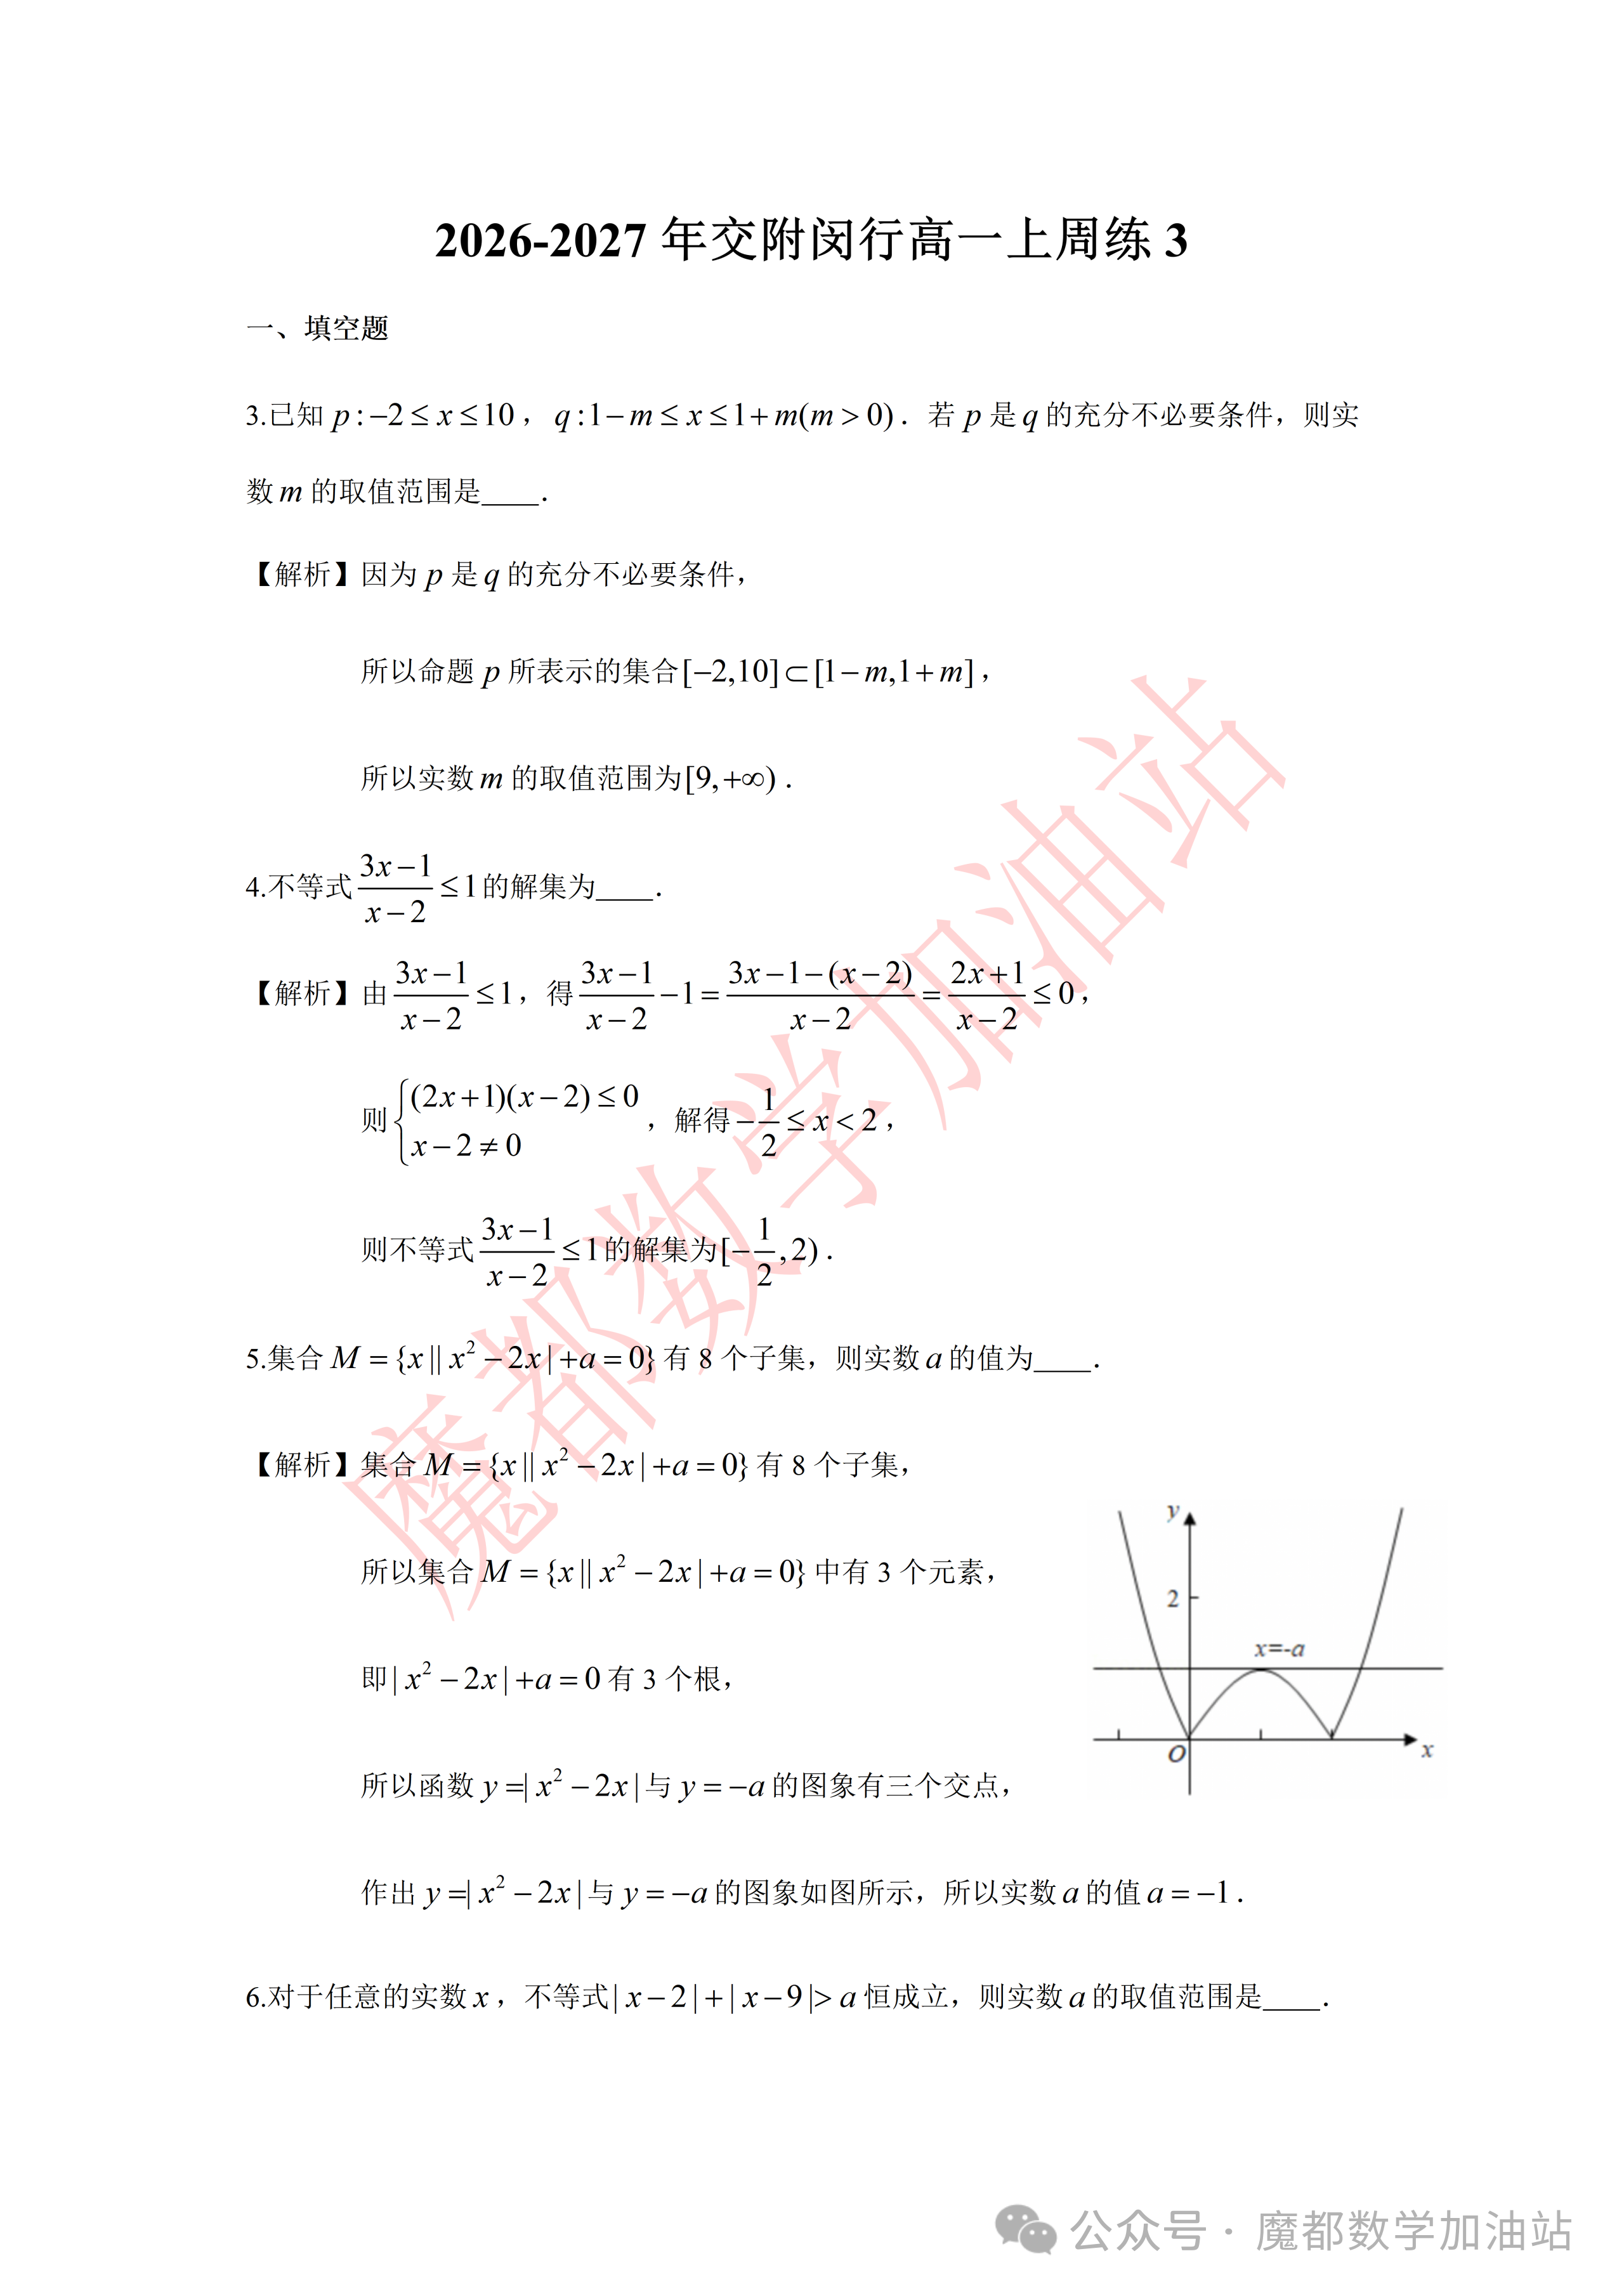
\includegraphics[width=0.14\textwidth,trim={1721bp 837bp 280bp 2297bp},clip]{../原图/高一43_交附闵行_周练3/01.png}
\end{center}

\solbegin
\step{集合 $M=\{x\mid |x^2-2x|+a=0\}$ 有 8 个子集，}
\step{所以集合 $M=\{x\mid |x^2-2x|+a=0\}$ 中有 3 个元素，}
\step{即 $|x^2-2x|+a=0$ 有 3 个根，}
\step{所以函数 $y=|x^2-2x|$ 与 $y=-a$ 的图象有三个交点，}
\step{作出 $y=|x^2-2x|$ 与 $y=-a$ 的图象如图所示，所以实数 $a$ 的值 $a=-1$.}
\solend

\fi

\item 对于任意的实数 $x$，不等式 $|x-2|+|x-9|>a$ 恒成立，则实数 $a$ 的取值范围是 \blankline[4.4em].

\ifanswer
\solbegin
\step{由绝对值的几何意义得 $|x-2|+|x-9|\geqslant7$，当且仅当 $2\leqslant x\leqslant9$ 时等号成立，}
\step{所以 $a<7$，}
\step{即 $a$ 的取值范围为 $(-\infty,7)$.}
\solend

\fi

\item 已知集合 $A=\{x\mid(a-1)x^2+3x-2=0\}$，$B=\{x\mid x^2-3x+2=0\}$，$A\subseteq B$，求实数 $a$ 的取值范围是 \blankline[4.4em].

\ifanswer
\solbegin
\step{由方程 $x^2-3x+2=0$，解得 $x=1$ 或 $x=2$，即 $B=\{1,2\}$，}
\step{因为 $A\subseteq B$，所以 $A=\varnothing$ 或 $A=\{1\}$ 或 $A=\{2\}$ 或 $A=\{1,2\}$，}
\step{当 $A=\varnothing$ 时，$a\neq1$，且 $\Delta=3^2-4(a-1)\times(-2)<0$，解得 $a<-\dfrac18$，}
\step{将 $x=1$ 代入方程 $(a-1)x^2+3x-2=0$，得 $a=0$，}
\step{此时 $A=\{x\mid-x^2+3x-2=0\}=\{1,2\}$，满足条件，}
\step{将 $x=2$ 代入方程 $(a-1)x^2+3x-2=0$，得到 $a=0$，上面已经验证满足条件，}
\step{综上所述，$a$ 的取值范围是 $\left(-\infty,-\dfrac18\right)\cup\{0\}$.}
\solend

\fi

\item 已知 $a$、$b$、$c$、$d$ 为常数，若不等式
$\dfrac{b}{x+a}+\dfrac{x+d}{x+c}<0$ 的解集为 $\left(-1,-\dfrac13\right)\cup\left(\dfrac12,1\right)$，
则不等式 $\dfrac{bx}{ax-1}+\dfrac{dx-1}{cx-1}<0$ 的解集为 \blankline[4.4em].

\ifanswer
\solbegin
\step{若 $x=0$，原不等式化为 $1<0$，不等式显然不成立，所以 $x\neq0$，}
\step{由 $\dfrac{bx}{ax-1}+\dfrac{dx-1}{cx-1}<0$，得 $\dfrac{b}{a-\dfrac1x}+\dfrac{d-\dfrac1x}{c-\dfrac1x}<0$，即 $\dfrac{b}{-\dfrac1x+a}+\dfrac{-\dfrac1x+d}{-\dfrac1x+c}<0$.}
\step{因为不等式 $\dfrac{b}{x+a}+\dfrac{x+d}{x+c}<0$ 的解集为 $\left(-1,-\dfrac13\right)\cup\left(\dfrac12,1\right)$，}
\step{所以 $-1<-\dfrac1x<-\dfrac13$ 或 $\dfrac12<-\dfrac1x<1$，解得 $1<x<3$ 或 $-2<x<-1$，}
\step{所以不等式 $\dfrac{bx}{ax-1}+\dfrac{dx-1}{cx-1}<0$ 的解集为 $(-2,-1)\cup(1,3)$.}
\solend

\fi

\item 正实数 $x$、$y$ 满足 $2x+3y-xy=0$，且存在这样的 $x$、$y$ 使不等式 $x+y<m+1$ 有解，则实数 $m$ 的取值范围是 \blankline[4.4em].

\ifanswer
\solbegin
\step{因为正实数 $x$、$y$ 满足 $2x+3y-xy=0$，则 $\dfrac2y+\dfrac3x=1$，$x>0$，$y>0$，}
\step{所以 $x+y=(x+y)\left(\dfrac3x+\dfrac2y\right)=3+\dfrac{2x}{y}+\dfrac{3y}{x}+2\geqslant2\sqrt{\dfrac{2x}{y}\times\dfrac{3y}{x}}+5=5+2\sqrt6$，}
\step{当且仅当 $\sqrt2x=\sqrt3y$ 时取等号，}
\step{存在这样的 $x$、$y$ 使不等式 $x+y<m+1$ 有解，则 $m+1>5+2\sqrt6$，}
\step{则 $m>4+2\sqrt6$，所以实数 $m$ 的取值范围是 $(4+2\sqrt6,+\infty)$.}
\solend

\fi

\item 若 $a$、$b$、$c\in\R$，$a^2+b^2+c^2=1$，则 $2ab+bc$ 的最大值为 \blankline[4.4em].

\ifanswer
\solbegin
\step{对于 $2ab+bc$，将 $b^2$ 拆分为 $\dfrac45b^2+\dfrac15b^2$，则 $a^2+\dfrac45b^2+c^2+\dfrac15b^2=1$，}
\step{$a^2+\dfrac45b^2\geqslant2\cdot a\cdot\dfrac2{\sqrt5}b=\dfrac4{\sqrt5}ab$，$c^2+\dfrac15b^2\geqslant2\cdot c\cdot\dfrac1{\sqrt5}b=\dfrac2{\sqrt5}bc$，}
\step{两式相加得 $1\geqslant\dfrac4{\sqrt5}ab+\dfrac2{\sqrt5}bc=\dfrac2{\sqrt5}(2ab+bc)$，故 $2ab+bc\leqslant\dfrac{\sqrt5}2$，}
\step{等号成立当且仅当 $a=\dfrac2{\sqrt5}b$，$c=\dfrac1{\sqrt5}b$，}
\step{代入 $a^2+b^2+c^2=1$，得 $\dfrac45b^2+b^2+\dfrac15b^2=2b^2=1$，即 $b=\dfrac{\sqrt2}2$，}
\step{此时 $a=\dfrac{\sqrt{10}}5$，$c=\dfrac{\sqrt{10}}{10}$，故 $2ab+bc$ 的最大值为 $\dfrac{\sqrt5}2$.}
\solend

\fi

\item 已知实数 $a$、$b$ 满足 $-3<a+2b<2$，$-1<2a-b<4$，则 $a+b$ 的取值范围为 \blankline[4.4em].

\ifanswer
\solbegin
\step{设 $a+b=m(a+2b)+n(2a-b)=(m+2n)a+(2m-n)b$，}
\step{所以 $\begin{cases}m+2n=1\\2m-n=1\end{cases}$，解得 $n=\dfrac15$，$m=\dfrac35$，所以 $a+b=\dfrac35(a+2b)+\dfrac15(2a-b)$，}
\step{因为 $-3<a+2b<2$，$-1<2a-b<4$，}
\step{所以 $-\dfrac95<\dfrac35(a+2b)<\dfrac65$，$-\dfrac15<\dfrac15(2a-b)<\dfrac45$，}
\step{相加得 $-2<\dfrac35(a+2b)+\dfrac15(2a-b)<2$，即 $-2<a+b<2$，}
\step{故 $a+b$ 的取值范围为 $(-2,2)$.}
\solend

\fi

% 注：原卷题干与解析均印作 \sqrt{2xyz}，但按其自身答案 8 与取等值（$y=\dfrac12$，
% $x=\dfrac{\sqrt3}4$，$z=\dfrac{\sqrt6}4$）代入只与 $\sqrt{2x^2y^2z^2}=\sqrt2\,xyz$ 相符，
% $\sqrt{2xyz}$ 与答案 8 不自洽，原卷如此，照录未改。
\item 已知正数 $x$、$y$、$z$ 满足 $2x^2+y^2+z^2=1$，则 $\dfrac{y+1}{\sqrt{2xyz}}$ 的最小值为 \blankline[4.4em].

\ifanswer
\solbegin
\step{由条件得 $2x^2+z^2=1-y^2=(1-y)(1+y)$，则 $1+y=\dfrac{2x^2+z^2}{1-y}$，}
\step{结合 $x$、$y$、$z>0$ 得原式 $=\dfrac{2x^2+z^2}{\sqrt{2xyz}(1-y)}\geqslant\dfrac{2\sqrt2xz}{\sqrt{2xyz}(1-y)}=\dfrac2{y(1-y)}$，}
\step{又 $y(1-y)\leqslant\left(\dfrac{y+1-y}2\right)^2=\dfrac14$，所以 $\dfrac2{y(1-y)}\geqslant\dfrac2{\frac14}=8$，}
\step{当且仅当 $\sqrt2x=z$，且 $y=1-y$，即 $y=\dfrac12$，$x=\dfrac{\sqrt3}4$，$z=\dfrac{\sqrt6}4$ 时取等号，}
\step{故 $\dfrac{y+1}{\sqrt{2xyz}}$ 最小值为 $8$.}
\solend

\fi

\end{enumerate}

\bigsec{二、选择题}

\begin{enumerate}
\setcounter{enumi}{12}

\item 已知关于 $x$ 的方程 $(1-k)x^2-2x-1=0$ 有实数根，则 $k$ 的取值范围是\mbox{（\quad）}

\keepwithprev
A. $k\leqslant2$ 且 $k\neq1$\qquad B. $k\leqslant2$\qquad
C. $k<2$ 且 $k\neq1$\qquad D. $k<2$

\ans{$A$}

\ifanswer
\solbegin
\step{由题意得 $\begin{cases}1-k\neq0\\\Delta=4+4(1-k)\geqslant0\end{cases}$，解不等式得 $\begin{cases}1\neq k\\2-k>0\end{cases}$，所以 $k\leqslant2$ 且 $k\neq1$，}
\step{故选 $A$.}
\solend

\fi

\item 不等式 $2|x+2|+|x-1|\geqslant5$ 成立的一个必要不充分条件是\mbox{（\quad）}

\keepwithprev
A. $x\leqslant-1$ 或 $x\geqslant0$\qquad B. $x\geqslant0$

C. $x\leqslant-\dfrac83$ 或 $x\geqslant0$\qquad D. $x\geqslant1$

\ans{$A$}

\ifanswer
\solbegin
\step{当 $x<-2$ 时，原不等式可化为 $-2x-4-x+1\geqslant5$，解得 $x\leqslant-\dfrac83$，}
\step{当 $-2\leqslant x<1$ 时，原不等式可化为 $2x+4-x+1\geqslant5$，解得 $0\leqslant x<1$，}
\step{当 $x\geqslant1$ 时，原不等式可化为 $2x+4+x-1\geqslant5$，解得 $x\geqslant\dfrac23$，得 $x\geqslant1$，}
\step{综上所述，不等式 $2|x+2|+|x-1|\geqslant5$ 成立的充要条件是 $x\leqslant-\dfrac83$ 或 $x\geqslant0$，}
\step{设 $A=\{x\mid x\leqslant-\dfrac83\text{ 或 }x\geqslant0\}$，}
\step{则不等式 $2|x+2|+|x-1|\geqslant5$ 成立的必要不充分条件，}
\step{其对应的集合 $B$ 满足 $A\subsetneq B$，对照各个选项，$A$ 项符合题意. 故选 $A$.}
\solend

\fi

\item 已知实数 $a>0$，$b>0$，$\dfrac1{a+1}+\dfrac1{b+1}=1$，则 $2a+3b$ 的最小值为\mbox{（\quad）}

\keepwithprev
A. $2\sqrt6$\qquad B. $3+2\sqrt6$\qquad
C. $5+2\sqrt6$\qquad D. $3+2\sqrt2$

\ans{$A$}

\ifanswer
\solbegin
\step{因为 $a>0$，$b>0$，$\dfrac1{a+1}+\dfrac1{b+1}=1$，}
\step{所以 $2a+3b=2(a+1)+3(b+1)-5=[2(a+1)+3(b+1)]\cdot\left(\dfrac1{a+1}+\dfrac1{b+1}\right)-5$}
\step{$=\left[2+3+\dfrac{3(b+1)}{a+1}+\dfrac{2(a+1)}{b+1}\right]-5\geqslant5+2\sqrt{\dfrac{3(b+1)}{a+1}\times\dfrac{2(a+1)}{b+1}}-5=2\sqrt6$，}
\step{当且仅当 $\dfrac{3(b+1)}{a+1}=\dfrac{2(a+1)}{b+1}$，即 $a=\dfrac{\sqrt6}2$，$b=\dfrac{\sqrt6}3$ 时取等号. 故选 $A$.}
\solend

\fi

\item 已知集合 $U=\{n\mid1\leqslant n\leqslant2027,\ n\in\N\}$，集合 $M\subseteq U$，若对于 $M$ 中任意两个不同的元素 $x$ 和 $y$，都有 $|x-y|>2$，则 $M$ 中元素个数的最大值是\mbox{（\quad）}

\keepwithprev
A. $676$\qquad B. $675$\qquad C. $672$\qquad D. $671$

\ans{$A$}

\ifanswer
\solbegin
\step{对于 $M$ 中的任意两个不同的元素 $x$、$y$，都有 $|x-y|>2$，}
\step{不妨设 $x>y$，都有 $x-y\geqslant3$，}
\step{要想 $M$ 所含元素个数最大，则要 $x-y$ 尽可能小，故需使得 $x-y$ 的最小值为 3，}
\step{将 $1\sim2027$ 这 2027 个元素按如下分组：}
\step{$\{1,2,3\}$，$\{4,5,6\}$，$\cdots$，$\{2023,2024,2025\}$，$\{2026,2027\}$，}
\step{故应在前 675 组中按周期 3 每组取一个元素，且第一组中不能取 3，}
\step{第一组中取 1 时，得 $M=\{1,4,7,\cdots,2023,2026\}$，}
\step{或 $M=\{1,4,7,\cdots,2023,2027\}$ 这样的集合，}
\step{第一组取 2 时，得 $M=\{2,5,8,\cdots,2024,2027\}$，}
\step{其中任意两元素差值 $x-y$（$x>y$）都大于 2，满足题意，}
\step{故 $M$ 所含元素个数的最大值为 $\dfrac{2025}{3}+1=676$. 故选 $A$.}
\solend

\fi

\end{enumerate}

\bigsec{三、解答题}

\begin{enumerate}
\setcounter{enumi}{16}

\item 已知 $a\in\R$，集合 $A=\left\{x\middle|\dfrac{2-x}{x+1}\leqslant0\right\}$，$B=\{x\mid x^2+(3-a)x-3a<0\}$.

\begin{enumerate}[label=(\arabic*)]
\item 当 $a=\dfrac13$ 时，求 $A$ 和 $B$；
\item 已知 $A\cup B=A$，求实数 $a$ 的取值范围.
\end{enumerate}

\ifanswer
\solbegin
\stepm{(1)}{由 $\dfrac{2-x}{x+1}\leqslant0$，得 $\begin{cases}(2-x)(x+1)\leqslant0\\x\neq-1\end{cases}$，解得 $x<-1$ 或 $x\geqslant2$，}
\step{则 $A=\{x\mid x<-1\text{ 或 }x\geqslant2\}$；}
\step{$B=\{x\mid x^2+(3-a)x-3a<0\}=\{x\mid(x+3)(x-a)<0\}$，}
% 注：原卷此行印作 $(x+2)\left(x-\dfrac13\right)$，按前一行 $B=\{x\mid(x+3)(x-a)<0\}$ 应为
% $(x+3)\left(x-\dfrac13\right)$，原卷如此，照录未改。
\step{当 $a=\dfrac13$ 时，$B=\left\{x\middle|(x+2)\left(x-\dfrac13\right)<0\right\}$，}
\step{解得 $B=\left\{x\middle|-3<x<\dfrac13\right\}$.}
\stepm{(2)}{由 $A\cup B=A$，得 $B\subseteq A$，}
\step{①当 $B=\varnothing$ 时，得 $a=-3$，符合题意；}
\step{②当 $B\neq\varnothing$ 时，若 $a>-3$，则 $B=\{x\mid-3<x<a\}$，}
\step{由 $B\subseteq A$，得 $a\leqslant-1$，此时 $-3<a\leqslant-1$；}
\step{若 $a<-3$，则 $B=\{x\mid a<x<-3\}$，此时 $B\subseteq A$ 恒成立，}
\step{故 $a<-3$ 符合题意；}
\step{综上所述，实数 $a$ 的取值范围为 $a\leqslant-1$.}
\solend

\fi

\ansspace[6]

\item 甲乙两地的高速公路全长 166 千米，汽车从甲地进入该高速公路后匀速行驶到乙地，车速 $v\in[70,120]$（千米/时）. 已知汽车每小时的运输成本（以元为单位）由可变部分和固定部分组成：可变部分为 $0.02v^2$，固定部分为 220 元.

\begin{enumerate}[label=(\arabic*)]
\item 若每小时的运输成本不高于 420 元，汽车的速度应该控制在什么范围？
\item 汽车应以多大速度行驶才能使全程运输成本最小？最小运输成本约为多少元？（结果保留整数）
\end{enumerate}

\ifanswer
\solbegin
\stepm{(1)}{已知汽车每小时的运输成本（以元为单位）由可变部分和固定部分组成：}
\step{可变部分为 $0.02v^2$，固定部分为 220 元，}
\step{则汽车每小时的运输成本为 $0.02v^2+220$（元），}
\step{若每小时的运输成本不高于 420 元，}
\step{则 $0.02v^2+220\leqslant420$，解得 $v^2\leqslant10000$，}
\step{得 $70\leqslant v\leqslant100$，即 $v\in[70,100]$（千米/时），}
\step{则此时汽车的速度 $v$ 应该控制在 $[70,100]$（千米/时）；}
\stepm{(2)}{因为汽车从甲地进入该高速公路后匀速行驶到乙地，}
\step{车速 $v\in[70,120]$（千米/时），所以汽车的行驶时间为 $\dfrac{166}{v}$（小时），}
\step{所以全程运输成本 $y=\dfrac{166}{v}(0.02v^2+220)=3.32v+\dfrac{36520}{v}$，}
% 注：原卷此行印作 $v\in[70,100]$，与题干的 $v\in[70,120]$ 不自洽（若 $v\in[70,100]$，
% 最小值应在 $v=100$ 处取得，与下文 $v=10\sqrt{110}\approx105$ 矛盾），原卷如此，照录未改。
\step{$v\in[70,100]$，}
\step{由基本不等式得 $y=3.32v+\dfrac{36520}{v}\geqslant2\sqrt{3.32v\times\dfrac{36520}{v}}\approx696$，}
\step{当且仅当 $3.32v=\dfrac{36520}{v}$，即 $v=10\sqrt{110}\approx105$ 时取等号，}
\step{汽车应以 105（千米/时）行驶才能使全程运输成本最小，}
\step{最小运输成本约为 696 元.}
\solend

\fi

\ansspace[8]

\item
\begin{enumerate}[label=(\arabic*)]
\item 已知 $a$、$b$、$c$ 为实数，求证：$|a-b|\leqslant|a-c|+|b-c|$，并说明等号成立的条件；
\item 设 $x\in\R$，求方程 $|3x-8|=|5-x|+|2x-3|$ 的解集.
\end{enumerate}

\ifanswer
% 注：原卷第 19 题未印【解析】，仅印一行【答案】"（1）(a-c)(b-c)≤0；
% （2）(-∞,3/2]∪[5,+∞)"。(1) 的两行推导为本稿所补，(2) 照录原卷答案。
% 又题干作"方程"，而所给答案 (-∞,3/2]∪[5,+∞) 实为不等式 |3x-8|≤|5-x|+|2x-3| 的解集，
% 与"方程"不合，原卷如此，照录未改。
\solbegin
\stepm{(1)}{由三角不等式 $|a-b|=|(a-c)-(b-c)|\leqslant|a-c|+|b-c|$，}
\step{当且仅当 $(a-c)(b-c)\leqslant0$ 时等号成立.}
\stepm{(2)}{$\left(-\infty,\dfrac32\right]\cup[5,+\infty)$.}
\solend

\fi

\ansspace[6]

\item 已知正实数 $a$、$b$ 满足 $a+b=1$，求 $\dfrac1a+\dfrac1b$ 的最小值. 其中一种解法是：

\[
\begin{aligned}
\dfrac1a+\dfrac1b
&=\left(\dfrac1a+\dfrac1b\right)(a+b)\\
&=1+\dfrac ba+\dfrac ab+1\\
&\geqslant2+2\sqrt{\dfrac ba\times\dfrac ab}=2+2=4.
\end{aligned}
\]
当且仅当 $\dfrac ba=\dfrac ab$ 且 $a+b=1$ 时即 $a=b=\dfrac12$ 时取等号.
学习上述解法并解决下列问题：

\begin{enumerate}[label=(\arabic*)]
\item 若正实数 $x$、$y$ 满足 $x+y=xy$，求 $2x+y$ 的最小值；
\item 若实数 $a$、$b$、$x$、$y$ 满足 $\dfrac{x^2}{a^2}+\dfrac{y^2}{b^2}=1$，求证：$a^2+b^2\geqslant(x+y)^2$；
\item 求代数式 $M=\sqrt{m-1}+\sqrt{3-m}$ 的最大值，并求出使得 $M$ 最大的 $m$ 的值.
\end{enumerate}

\ifanswer
\solbegin
\stepm{(1)}{因为正实数 $x$、$y$ 满足 $x+y=xy$，$\dfrac{x+y}{xy}=1\Rightarrow\dfrac1y+\dfrac1x=1$，}
\step{所以 $(2x+y)\times1=(2x+y)\left(\dfrac1y+\dfrac1x\right)=3+\dfrac{2x}{y}+\dfrac yx\geqslant3+2\sqrt{\dfrac{2x}{y}\cdot\dfrac yx}=3+2\sqrt2$，}
\step{当且仅当 $\dfrac{2x}{y}=\dfrac yx$ 且 $\dfrac1y+\dfrac1x=1$ 时取等号，}
\step{解得 $x=\dfrac{2+\sqrt2}2$，$y=\sqrt2x=\sqrt2\times\dfrac{2+\sqrt2}2=1+\sqrt2$，}
\step{所以 $2x+y$ 的最小值为 $3+2\sqrt2$；}
\stepm{(2)}{因为 $\dfrac{x^2}{a^2}+\dfrac{y^2}{b^2}=1$，}
\step{所以 $a^2+b^2=(a^2+b^2)\left(\dfrac{x^2}{a^2}+\dfrac{y^2}{b^2}\right)=x^2+y^2+\dfrac{b^2x^2}{a^2}+\dfrac{a^2y^2}{b^2}$，}
\step{因为 $\dfrac{b^2x^2}{a^2}+\dfrac{a^2y^2}{b^2}\geqslant2\sqrt{\dfrac{b^2x^2}{a^2}\times\dfrac{a^2y^2}{b^2}}=2\sqrt{x^2y^2}=2|xy|$，}
\step{当且仅当 $\dfrac{b^2x^2}{a^2}=\dfrac{a^2y^2}{b^2}$ 时取等号，}
\step{所以 $x^2+y^2+\dfrac{b^2x^2}{a^2}+\dfrac{a^2y^2}{b^2}\geqslant x^2+y^2+2|xy|\geqslant x^2+y^2+2xy=(x+y)^2$，}
\step{所以 $a^2+b^2\geqslant(x+y)^2$；}
\stepm{(3)}{因为 $M=\sqrt{m-1}+\sqrt{3-m}$，所以 $\begin{cases}m-1\geqslant0\\3-m\geqslant0\end{cases}$，解得 $1\leqslant m\leqslant3$，}
\step{所以 $M^2=(\sqrt{m-1}+\sqrt{3-m})^2=2+2\sqrt{(3-m)(m-1)}$，}
\step{由基本不等式得 $(3-m)(m-1)\leqslant\left(\dfrac{(3-m)+(m-1)}2\right)^2=1$，}
\step{当且仅当 $3-m=m-1$ 时取等号，解得 $m=2$，}
\step{所以 $M^2=2+2\sqrt{(3-m)(m-1)}\leqslant2+2\sqrt1=4$，}
\step{因为 $M>0$，所以 $M\leqslant2$，所以 $M$ 最大值为 2，此时 $m$ 的值为 2.}
\solend

\fi

\ansspace[8]

\item 若有限个正整数组成的集合 $A$ 中至少有两个元素，且对于任意的 $x,y\in A$（$x>y$），都有 $\dfrac{y^2}{x-y}\in A$，则称 $A$ 为“L-集合”.

\begin{enumerate}[label=(\arabic*)]
\item 判断 $\{1,2,4\}$ 是否为“L-集合”，说明理由；
\item 若双元素集 $M$ 为“L-集合”，且 $4\in M$，求所有满足条件的集合 $M$；
\item 求所有满足条件的“L-集合”.
\end{enumerate}

\ifanswer
\solbegin
\stepm{(1)}{若至少由两个元素构成的有限集合 $A\subseteq\N^*$，}
% 注：原卷下一行"都有"后未印分数 \dfrac{y^2}{x-y}，径作"都有 A"，原卷如此，照录未改。
\step{且对于任意的 $x$、$y\in A$（$x>y$），都有 $A$，则称 $A$ 为“L-集合”，}
\step{$\{1,2,4\}$ 不为“L-集合”，理由如下：}
\step{因为 $\dfrac{1^2}{4-1}=\dfrac13\notin\{1,2,4\}$，所以 $\{1,2,4\}$ 不是“L-集合”.}
\stepm{(2)}{设 $M=\{4,m\}$（$m\in\N^*$，$m\neq4$），}
\step{若 $m<4$，则 $\dfrac{m^2}{4-m}=m$ 或 $\dfrac{m^2}{4-m}=4$，}
\step{由 $\dfrac{m^2}{4-m}=m$，解得 $m=2$，$m=0$（舍去），此时 $M=\{2,4\}$；}
\step{由 $\dfrac{m^2}{4-m}=4$ 化为 $m^2+4m-16=0$，而 $\Delta=4^2+4\times16=80$，}
\step{故方程无正整数解.}
\step{若 $m>4$，则 $\dfrac{4^2}{m-4}=4$ 或 $\dfrac{4^2}{m-4}=m$，}
\step{由 $\dfrac{4^2}{m-4}=4$，解得 $m=8$，此时 $M=\{4,8\}$；}
\step{由 $\dfrac{4^2}{m-4}=m$ 化为 $m^2-4m-16=0$，而 $\Delta=4^2+4\times16=80$，}
\step{故方程无正整数解.}
\step{综上，双元素集 $M$ 为“L-集合”，且 $4\in M$，}
\step{则所有满足条件的集合 $M$ 为 $\{4,8\}$，$\{2,4\}$.}
\stepm{(3)}{若“L-集合”为双元素集，}
\step{不妨设 $M=\{k,m\}$（$k,m\in\N^*$，$m>k$），则 $\dfrac{k^2}{m-k}=k$ 或 $\dfrac{k^2}{m-k}=m$，}
\step{由 $\dfrac{k^2}{m-k}=k$，则 $2k^2=mk$，而 $m>k$，故 $m=2k$，此时 $M=\{k,2k\}$；}
\step{由 $\dfrac{k^2}{m-k}=m$，则 $m^2-mk-k^2=0$，而 $\Delta=5k^2$，显然不存在正整数解；}
\step{所以，“L-集合”为 $\{k,2k\}$，其中 $k\in\N^*$.}
\step{若“L-集合”含有两个以上的元素，}
\step{设最小的元素为 $b$，最大的元素为 $a$，第二大的元素为 $n$，}
\step{则 $\dfrac{b^2}{a-b}$，$\dfrac{n^2}{a-n}$ 是“L-集合”中的元素，}
% 注：原卷下一行未印"由于'L-集合'中的元素均为正整数"一语，径作"若 \dfrac{b^2}{a-b}\geqslant b"，
% 原卷如此，照录未改。
\step{若 $\dfrac{b^2}{a-b}\geqslant b$，解得 $a\leqslant2b$，}
\step{若 $\dfrac{n^2}{a-n}\leqslant n$，则 $a\geqslant2n>2b$，矛盾，}
\step{若 $\dfrac{n^2}{a-n}=a$，该方程的解为 $n=\dfrac{\sqrt5-1}2a$，则 $n$、$a$ 不可能同时为整数，}
\step{无解.}
\step{所以所有满足条件的“L-集合”为 $\{k,2k\}$，其中 $k\in\N^*$.}
\solend

\fi

\ansspace*[10]

\end{enumerate}

\end{document}
